\documentclass{book}
\usepackage[a4paper,top=2.5cm,bottom=2.5cm,left=2.5cm,right=2.5cm]{geometry}
\usepackage{makeidx}
\usepackage{natbib}
\usepackage{graphicx}
\usepackage{multicol}
\usepackage{float}
\usepackage{listings}
\usepackage{color}
\usepackage{ifthen}
\usepackage[table]{xcolor}
\usepackage{textcomp}
\usepackage{alltt}
\usepackage{ifpdf}
\ifpdf
\usepackage[pdftex,
            pagebackref=true,
            colorlinks=true,
            linkcolor=blue,
            unicode
           ]{hyperref}
\else
\usepackage[ps2pdf,
            pagebackref=true,
            colorlinks=true,
            linkcolor=blue,
            unicode
           ]{hyperref}
\usepackage{pspicture}
\fi
\usepackage[utf8]{inputenc}
\usepackage{mathptmx}
\usepackage[scaled=.90]{helvet}
\usepackage{courier}
\usepackage{sectsty}
\usepackage{amssymb}
\usepackage[titles]{tocloft}
\usepackage{doxygen}
\lstset{language=C++,inputencoding=utf8,basicstyle=\footnotesize,breaklines=true,breakatwhitespace=true,tabsize=4,numbers=left }
\makeindex
\setcounter{tocdepth}{3}
\renewcommand{\footrulewidth}{0.4pt}
\renewcommand{\familydefault}{\sfdefault}
\hfuzz=15pt
\setlength{\emergencystretch}{15pt}
\hbadness=750
\tolerance=750
\begin{document}
\hypersetup{pageanchor=false,citecolor=blue}
\begin{titlepage}
\vspace*{7cm}
\begin{center}
{\Large X\-T\-D }\\
\vspace*{1cm}
{\large Generated by Doxygen 1.8.1.2}\\
\vspace*{0.5cm}
{\small Thu Aug 7 2014 15:57:07}\\
\end{center}
\end{titlepage}
\clearemptydoublepage
\pagenumbering{roman}
\tableofcontents
\clearemptydoublepage
\pagenumbering{arabic}
\hypersetup{pageanchor=true,citecolor=blue}
\chapter{Namespace Index}
\section{Namespace List}
Here is a list of all documented namespaces with brief descriptions\-:\begin{DoxyCompactList}
\item\contentsline{section}{\hyperlink{namespacestr}{str} \\*A namespace containing tools for operations which strings }{\pageref{namespacestr}}{}
\item\contentsline{section}{\hyperlink{namespacextd}{xtd} \\*A root namespace of the library }{\pageref{namespacextd}}{}
\end{DoxyCompactList}

\chapter{Class Index}
\section{Class Hierarchy}
This inheritance list is sorted roughly, but not completely, alphabetically\-:\begin{DoxyCompactList}
\item \contentsline{section}{xstd\-:\-:abstract\-\_\-functor$<$ arguments\-\_\-type $>$}{\pageref{classxstd_1_1abstract__functor}}{}
\item \contentsline{section}{xstd\-:\-:abstract\-\_\-functor$<$ arguments\-\_\-type...$>$}{\pageref{classxstd_1_1abstract__functor}}{}
\begin{DoxyCompactList}
\item \contentsline{section}{xstd\-:\-:functor$<$ object\-\_\-type, arguments\-\_\-type $>$}{\pageref{classxstd_1_1functor}}{}
\end{DoxyCompactList}
\item \contentsline{section}{xstd\-:\-:abstract\-\_\-logger}{\pageref{classxstd_1_1abstract__logger}}{}
\begin{DoxyCompactList}
\item \contentsline{section}{xstd\-:\-:console\-\_\-logger}{\pageref{classxstd_1_1console__logger}}{}
\item \contentsline{section}{xstd\-:\-:file\-\_\-logger}{\pageref{classxstd_1_1file__logger}}{}
\end{DoxyCompactList}
\item \contentsline{section}{xstd\-:\-:coutmt\-\_\-singleton}{\pageref{classxstd_1_1coutmt__singleton}}{}
\item \contentsline{section}{xstd\-:\-:dimension\-\_\-mismatch}{\pageref{structxstd_1_1dimension__mismatch}}{}
\item \contentsline{section}{xstd\-:\-:event$<$ data\-\_\-type $>$}{\pageref{classxstd_1_1event}}{}
\item \contentsline{section}{xstd\-:\-:pp\-:\-:first\-\_\-type$<$ parameters\-\_\-types $>$}{\pageref{structxstd_1_1pp_1_1first__type}}{}
\item \contentsline{section}{xstd\-:\-:pp\-:\-:is\-\_\-heterogeneous$<$ parameters\-\_\-types $>$}{\pageref{structxstd_1_1pp_1_1is__heterogeneous}}{}
\item \contentsline{section}{xstd\-:\-:pp\-:\-:is\-\_\-homogeneous$<$ parameters\-\_\-types $>$}{\pageref{structxstd_1_1pp_1_1is__homogeneous}}{}
\item \contentsline{section}{xstd\-:\-:pp\-:\-:is\-\_\-homogeneous$<$ first\-\_\-parameter\-\_\-type, other\-\_\-parameters\-\_\-types... $>$}{\pageref{structxstd_1_1pp_1_1is__homogeneous_3_01first__parameter__type_00_01other__parameters__types_8_8_8_01_4}}{}
\item \contentsline{section}{xstd\-:\-:pp\-:\-:is\-\_\-homogeneous$<$ parameter\-\_\-type $>$}{\pageref{structxstd_1_1pp_1_1is__homogeneous_3_01parameter__type_01_4}}{}
\item \contentsline{section}{xstd\-:\-:pp\-:\-:last\-\_\-type$<$ parameters\-\_\-types $>$}{\pageref{structxstd_1_1pp_1_1last__type}}{}
\item \contentsline{section}{xstd\-:\-:logger\-\_\-client}{\pageref{classxstd_1_1logger__client}}{}
\item \contentsline{section}{xstd\-:\-:pp\-:\-:nth\-\_\-type$<$ parameter\-\_\-id, parameters\-\_\-types $>$}{\pageref{structxstd_1_1pp_1_1nth__type}}{}
\item \contentsline{section}{xstd\-:\-:pp\-:\-:nth\-\_\-type\-\_\-helper$<$ parameter\-\_\-id, parameters\-\_\-types $>$}{\pageref{structxstd_1_1pp_1_1nth__type__helper}}{}
\item \contentsline{section}{xstd\-:\-:pp\-:\-:nth\-\_\-type\-\_\-helper$<$ 0, first\-\_\-parameter\-\_\-type, other\-\_\-parameters\-\_\-types... $>$}{\pageref{structxstd_1_1pp_1_1nth__type__helper_3_010_00_01first__parameter__type_00_01other__parameters__types_8_8_8_01_4}}{}
\item \contentsline{section}{xstd\-:\-:pp\-:\-:nth\-\_\-type\-\_\-helper$<$ parameter\-\_\-id, first\-\_\-parameter\-\_\-type, other\-\_\-parameters\-\_\-types... $>$}{\pageref{structxstd_1_1pp_1_1nth__type__helper_3_01parameter__id_00_01first__parameter__type_00_01other__parameters__types_8_8_8_01_4}}{}
\item \contentsline{section}{xstd\-:\-:pp\-:\-:null\-\_\-type}{\pageref{structxstd_1_1pp_1_1null__type}}{}
\item \contentsline{section}{xstd\-:\-:point$<$ type, dimension $>$}{\pageref{classxstd_1_1point}}{}
\item \contentsline{section}{printer}{\pageref{structprinter}}{}
\item \contentsline{section}{xstd\-:\-:raii\-\_\-thread\-\_\-base}{\pageref{classxstd_1_1raii__thread__base}}{}
\begin{DoxyCompactList}
\item \contentsline{section}{xstd\-:\-:raii\-\_\-thread}{\pageref{classxstd_1_1raii__thread}}{}
\item \contentsline{section}{xstd\-:\-:raii\-\_\-thread\-\_\-manual}{\pageref{classxstd_1_1raii__thread__manual}}{}
\end{DoxyCompactList}
\item \contentsline{section}{xstd\-:\-:chrono\-:\-:timer\-\_\-base}{\pageref{classxstd_1_1chrono_1_1timer__base}}{}
\begin{DoxyCompactList}
\item \contentsline{section}{xstd\-:\-:chrono\-:\-:timer$<$ clock $>$}{\pageref{classxstd_1_1chrono_1_1timer}}{}
\end{DoxyCompactList}
\item \contentsline{section}{xstd\-:\-:chrono\-:\-:timer\-\_\-manager}{\pageref{classxstd_1_1chrono_1_1timer__manager}}{}
\end{DoxyCompactList}

\chapter{Class Index}
\section{Class List}
Here are the classes, structs, unions and interfaces with brief descriptions\-:\begin{DoxyCompactList}
\item\contentsline{section}{\hyperlink{classxstd_1_1abstract__functor}{xstd\-::abstract\-\_\-functor$<$ arguments\-\_\-type $>$} }{\pageref{classxstd_1_1abstract__functor}}{}
\item\contentsline{section}{\hyperlink{classxstd_1_1abstract__logger}{xstd\-::abstract\-\_\-logger} }{\pageref{classxstd_1_1abstract__logger}}{}
\item\contentsline{section}{\hyperlink{classxstd_1_1console__logger}{xstd\-::console\-\_\-logger} }{\pageref{classxstd_1_1console__logger}}{}
\item\contentsline{section}{\hyperlink{classxstd_1_1coutmt__singleton}{xstd\-::coutmt\-\_\-singleton} }{\pageref{classxstd_1_1coutmt__singleton}}{}
\item\contentsline{section}{\hyperlink{structxstd_1_1dimension__mismatch}{xstd\-::dimension\-\_\-mismatch} }{\pageref{structxstd_1_1dimension__mismatch}}{}
\item\contentsline{section}{\hyperlink{classxstd_1_1event}{xstd\-::event$<$ data\-\_\-type $>$} }{\pageref{classxstd_1_1event}}{}
\item\contentsline{section}{\hyperlink{classxstd_1_1file__logger}{xstd\-::file\-\_\-logger} }{\pageref{classxstd_1_1file__logger}}{}
\item\contentsline{section}{\hyperlink{structxstd_1_1pp_1_1first__type}{xstd\-::pp\-::first\-\_\-type$<$ parameters\-\_\-types $>$} }{\pageref{structxstd_1_1pp_1_1first__type}}{}
\item\contentsline{section}{\hyperlink{classxstd_1_1functor}{xstd\-::functor$<$ object\-\_\-type, arguments\-\_\-type $>$} }{\pageref{classxstd_1_1functor}}{}
\item\contentsline{section}{\hyperlink{structxstd_1_1pp_1_1is__heterogeneous}{xstd\-::pp\-::is\-\_\-heterogeneous$<$ parameters\-\_\-types $>$} }{\pageref{structxstd_1_1pp_1_1is__heterogeneous}}{}
\item\contentsline{section}{\hyperlink{structxstd_1_1pp_1_1is__homogeneous}{xstd\-::pp\-::is\-\_\-homogeneous$<$ parameters\-\_\-types $>$} }{\pageref{structxstd_1_1pp_1_1is__homogeneous}}{}
\item\contentsline{section}{\hyperlink{structxstd_1_1pp_1_1is__homogeneous_3_01first__parameter__type_00_01other__parameters__types_8_8_8_01_4}{xstd\-::pp\-::is\-\_\-homogeneous$<$ first\-\_\-parameter\-\_\-type, other\-\_\-parameters\-\_\-types... $>$} }{\pageref{structxstd_1_1pp_1_1is__homogeneous_3_01first__parameter__type_00_01other__parameters__types_8_8_8_01_4}}{}
\item\contentsline{section}{\hyperlink{structxstd_1_1pp_1_1is__homogeneous_3_01parameter__type_01_4}{xstd\-::pp\-::is\-\_\-homogeneous$<$ parameter\-\_\-type $>$} }{\pageref{structxstd_1_1pp_1_1is__homogeneous_3_01parameter__type_01_4}}{}
\item\contentsline{section}{\hyperlink{structxstd_1_1pp_1_1last__type}{xstd\-::pp\-::last\-\_\-type$<$ parameters\-\_\-types $>$} }{\pageref{structxstd_1_1pp_1_1last__type}}{}
\item\contentsline{section}{\hyperlink{classxstd_1_1logger__client}{xstd\-::logger\-\_\-client} }{\pageref{classxstd_1_1logger__client}}{}
\item\contentsline{section}{\hyperlink{structxstd_1_1pp_1_1nth__type}{xstd\-::pp\-::nth\-\_\-type$<$ parameter\-\_\-id, parameters\-\_\-types $>$} }{\pageref{structxstd_1_1pp_1_1nth__type}}{}
\item\contentsline{section}{\hyperlink{structxstd_1_1pp_1_1nth__type__helper}{xstd\-::pp\-::nth\-\_\-type\-\_\-helper$<$ parameter\-\_\-id, parameters\-\_\-types $>$} }{\pageref{structxstd_1_1pp_1_1nth__type__helper}}{}
\item\contentsline{section}{\hyperlink{structxstd_1_1pp_1_1nth__type__helper_3_010_00_01first__parameter__type_00_01other__parameters__types_8_8_8_01_4}{xstd\-::pp\-::nth\-\_\-type\-\_\-helper$<$ 0, first\-\_\-parameter\-\_\-type, other\-\_\-parameters\-\_\-types... $>$} }{\pageref{structxstd_1_1pp_1_1nth__type__helper_3_010_00_01first__parameter__type_00_01other__parameters__types_8_8_8_01_4}}{}
\item\contentsline{section}{\hyperlink{structxstd_1_1pp_1_1nth__type__helper_3_01parameter__id_00_01first__parameter__type_00_01other__parameters__types_8_8_8_01_4}{xstd\-::pp\-::nth\-\_\-type\-\_\-helper$<$ parameter\-\_\-id, first\-\_\-parameter\-\_\-type, other\-\_\-parameters\-\_\-types... $>$} }{\pageref{structxstd_1_1pp_1_1nth__type__helper_3_01parameter__id_00_01first__parameter__type_00_01other__parameters__types_8_8_8_01_4}}{}
\item\contentsline{section}{\hyperlink{structxstd_1_1pp_1_1null__type}{xstd\-::pp\-::null\-\_\-type} }{\pageref{structxstd_1_1pp_1_1null__type}}{}
\item\contentsline{section}{\hyperlink{classxstd_1_1point}{xstd\-::point$<$ type, dimension $>$} }{\pageref{classxstd_1_1point}}{}
\item\contentsline{section}{\hyperlink{structprinter}{printer} }{\pageref{structprinter}}{}
\item\contentsline{section}{\hyperlink{classxstd_1_1raii__thread}{xstd\-::raii\-\_\-thread} }{\pageref{classxstd_1_1raii__thread}}{}
\item\contentsline{section}{\hyperlink{classxstd_1_1raii__thread__base}{xstd\-::raii\-\_\-thread\-\_\-base} }{\pageref{classxstd_1_1raii__thread__base}}{}
\item\contentsline{section}{\hyperlink{classxstd_1_1raii__thread__manual}{xstd\-::raii\-\_\-thread\-\_\-manual} }{\pageref{classxstd_1_1raii__thread__manual}}{}
\item\contentsline{section}{\hyperlink{classxstd_1_1chrono_1_1timer}{xstd\-::chrono\-::timer$<$ clock $>$} }{\pageref{classxstd_1_1chrono_1_1timer}}{}
\item\contentsline{section}{\hyperlink{classxstd_1_1chrono_1_1timer__base}{xstd\-::chrono\-::timer\-\_\-base} }{\pageref{classxstd_1_1chrono_1_1timer__base}}{}
\item\contentsline{section}{\hyperlink{classxstd_1_1chrono_1_1timer__manager}{xstd\-::chrono\-::timer\-\_\-manager} }{\pageref{classxstd_1_1chrono_1_1timer__manager}}{}
\end{DoxyCompactList}

\chapter{File Index}
\section{File List}
Here is a list of all documented files with brief descriptions\-:\begin{DoxyCompactList}
\item\contentsline{section}{src/chrono/chrono\-\_\-util/src/{\bfseries chrono\-\_\-util.\-hpp} }{\pageref{chrono__util_8hpp}}{}
\item\contentsline{section}{src/chrono/timer/timer/src/{\bfseries timer.\-hpp} }{\pageref{timer_8hpp}}{}
\item\contentsline{section}{src/chrono/timer/timer\-\_\-base/src/{\bfseries timer\-\_\-base.\-hpp} }{\pageref{timer__base_8hpp}}{}
\item\contentsline{section}{src/chrono/timer/timer\-\_\-manager/src/{\bfseries timer\-\_\-manager.\-hpp} }{\pageref{timer__manager_8hpp}}{}
\item\contentsline{section}{src/cmath/point/src/{\bfseries point.\-hpp} }{\pageref{point_8hpp}}{}
\item\contentsline{section}{src/cmath/random/src/{\bfseries random.\-hpp} }{\pageref{random_8hpp}}{}
\item\contentsline{section}{src/event/event/src/{\bfseries event.\-hpp} }{\pageref{event_8hpp}}{}
\item\contentsline{section}{src/fs/file\-\_\-util/src/{\bfseries file\-\_\-util.\-hpp} }{\pageref{file__util_8hpp}}{}
\item\contentsline{section}{src/functional/functor/abstract\-\_\-functor/src/{\bfseries abstract\-\_\-functor.\-hpp} }{\pageref{abstract__functor_8hpp}}{}
\item\contentsline{section}{src/functional/functor/functor/src/{\bfseries functor.\-hpp} }{\pageref{functor_8hpp}}{}
\item\contentsline{section}{src/iostream/coutmt/src/{\bfseries coutmt.\-hpp} }{\pageref{coutmt_8hpp}}{}
\item\contentsline{section}{src/log/abstract\-\_\-logger/src/{\bfseries abstract\-\_\-logger.\-hpp} }{\pageref{abstract__logger_8hpp}}{}
\item\contentsline{section}{src/log/console\-\_\-logger/src/{\bfseries console\-\_\-logger.\-hpp} }{\pageref{console__logger_8hpp}}{}
\item\contentsline{section}{src/log/file\-\_\-logger/src/{\bfseries file\-\_\-logger.\-hpp} }{\pageref{file__logger_8hpp}}{}
\item\contentsline{section}{src/log/logger\-\_\-client/src/{\bfseries logger\-\_\-client.\-hpp} }{\pageref{logger__client_8hpp}}{}
\item\contentsline{section}{src/memory/memory\-\_\-util/src/{\bfseries memory\-\_\-util.\-hpp} }{\pageref{memory__util_8hpp}}{}
\item\contentsline{section}{src/string/string\-\_\-util/src/\hyperlink{string__util_8hpp}{string\-\_\-util.\-hpp} }{\pageref{string__util_8hpp}}{}
\item\contentsline{section}{src/thread/raii\-\_\-thread/src/{\bfseries raii\-\_\-thread.\-hpp} }{\pageref{raii__thread_8hpp}}{}
\item\contentsline{section}{src/thread/raii\-\_\-thread\-\_\-base/src/{\bfseries raii\-\_\-thread\-\_\-base.\-hpp} }{\pageref{raii__thread__base_8hpp}}{}
\item\contentsline{section}{src/thread/raii\-\_\-thread\-\_\-manual/src/{\bfseries raii\-\_\-thread\-\_\-manual.\-hpp} }{\pageref{raii__thread__manual_8hpp}}{}
\item\contentsline{section}{src/utility/parameter\-\_\-pack/parameter\-\_\-pack\-\_\-element\-\_\-type/src/{\bfseries parameter\-\_\-pack\-\_\-element\-\_\-type.\-hpp} }{\pageref{parameter__pack__element__type_8hpp}}{}
\item\contentsline{section}{src/utility/parameter\-\_\-pack/parameter\-\_\-pack\-\_\-element\-\_\-value/src/{\bfseries parameter\-\_\-pack\-\_\-element\-\_\-value.\-hpp} }{\pageref{parameter__pack__element__value_8hpp}}{}
\item\contentsline{section}{src/utility/parameter\-\_\-pack/parameter\-\_\-pack\-\_\-for\-\_\-each/src/{\bfseries parameter\-\_\-pack\-\_\-for\-\_\-each.\-hpp} }{\pageref{parameter__pack__for__each_8hpp}}{}
\item\contentsline{section}{src/utility/parameter\-\_\-pack/parameter\-\_\-pack\-\_\-homogeneity/src/{\bfseries parameter\-\_\-pack\-\_\-homogeneity.\-hpp} }{\pageref{parameter__pack__homogeneity_8hpp}}{}
\end{DoxyCompactList}

\chapter{Namespace Documentation}
\hypertarget{namespacestr}{\section{str Namespace Reference}
\label{namespacestr}\index{str@{str}}
}


A namespace containing tools for operations which strings.  




\subsection{Detailed Description}
A namespace containing tools for operations which strings. 
\hypertarget{namespacexstd}{\section{xstd Namespace Reference}
\label{namespacexstd}\index{xstd@{xstd}}
}
\subsection*{Namespaces}
\begin{DoxyCompactItemize}
\item 
namespace \hyperlink{namespacexstd_1_1chrono}{chrono}
\item 
namespace \hyperlink{namespacexstd_1_1fs}{fs}
\item 
namespace \hyperlink{namespacexstd_1_1pp}{pp}
\item 
namespace \hyperlink{namespacexstd_1_1random}{random}
\end{DoxyCompactItemize}
\subsection*{Classes}
\begin{DoxyCompactItemize}
\item 
struct \hyperlink{structxstd_1_1dimension__mismatch}{dimension\-\_\-mismatch}
\item 
class \hyperlink{classxstd_1_1point}{point}
\item 
class \hyperlink{classxstd_1_1event}{event}
\item 
class \hyperlink{classxstd_1_1abstract__functor}{abstract\-\_\-functor}
\item 
class \hyperlink{classxstd_1_1functor}{functor}
\item 
class \hyperlink{classxstd_1_1coutmt__singleton}{coutmt\-\_\-singleton}
\item 
class \hyperlink{classxstd_1_1abstract__logger}{abstract\-\_\-logger}
\item 
class \hyperlink{classxstd_1_1console__logger}{console\-\_\-logger}
\item 
class \hyperlink{classxstd_1_1file__logger}{file\-\_\-logger}
\item 
class \hyperlink{classxstd_1_1logger__client}{logger\-\_\-client}
\item 
class \hyperlink{classxstd_1_1raii__thread}{raii\-\_\-thread}
\item 
class \hyperlink{classxstd_1_1raii__thread__base}{raii\-\_\-thread\-\_\-base}
\item 
class \hyperlink{classxstd_1_1raii__thread__manual}{raii\-\_\-thread\-\_\-manual}
\end{DoxyCompactItemize}
\subsection*{Typedefs}
\begin{DoxyCompactItemize}
\item 
typedef \hyperlink{classxstd_1_1point}{point}$<$ int, 2 $>$ \hyperlink{namespacexstd_a05f630b2b093cec28fcdd96aca897f75}{point\-\_\-i2}
\item 
typedef \hyperlink{classxstd_1_1point}{point}$<$ int, 3 $>$ \hyperlink{namespacexstd_a28fb4f569d80e07173722c8cc3465f81}{point\-\_\-i3}
\item 
typedef \hyperlink{classxstd_1_1point}{point}$<$ float, 2 $>$ \hyperlink{namespacexstd_aa26f7d45c70ace7cd0722a5d5d89dcd8}{point\-\_\-f2}
\item 
typedef \hyperlink{classxstd_1_1point}{point}$<$ float, 3 $>$ \hyperlink{namespacexstd_ac9dcb9387fb1c6f4f82773a54bfa5843}{point\-\_\-f3}
\end{DoxyCompactItemize}
\subsection*{Functions}
\begin{DoxyCompactItemize}
\item 
{\footnotesize template$<$typename Type $>$ }\\\hyperlink{classxstd_1_1coutmt__singleton}{coutmt\-\_\-singleton} \& \hyperlink{namespacexstd_a1e84f1aca8ea660c6b6857dd74e23095}{operator$<$$<$} (\hyperlink{classxstd_1_1coutmt__singleton}{coutmt\-\_\-singleton} \&coutmt\-\_\-singleton\-\_\-instance, Type object)
\item 
\hyperlink{classxstd_1_1coutmt__singleton}{coutmt\-\_\-singleton} \& \hyperlink{namespacexstd_a4ca9ff5b467cc2d187627f25fe4becb9}{operator$<$$<$} (\hyperlink{classxstd_1_1coutmt__singleton}{coutmt\-\_\-singleton} \&coutmt\-\_\-singleton\-\_\-instance, std\-::ostream \&($\ast$function\-\_\-ptr)(std\-::ostream \&))
\item 
\hyperlink{classxstd_1_1coutmt__singleton}{coutmt\-\_\-singleton} \& \hyperlink{namespacexstd_ae5a5bddbedf675617d11176fea8fee8b}{operator$<$$<$} (\hyperlink{classxstd_1_1coutmt__singleton}{coutmt\-\_\-singleton} \&coutmt\-\_\-singleton\-\_\-instance, std\-::ios \&($\ast$function\-\_\-ptr)(std\-::ios \&))
\item 
\hyperlink{classxstd_1_1coutmt__singleton}{coutmt\-\_\-singleton} \& \hyperlink{namespacexstd_a05baea78d624e383708fa5f4ba944f8e}{operator$<$$<$} (\hyperlink{classxstd_1_1coutmt__singleton}{coutmt\-\_\-singleton} \&coutmt\-\_\-singleton\-\_\-instance, std\-::ios\-\_\-base \&($\ast$function\-\_\-ptr)(std\-::ios\-\_\-base \&))
\item 
{\footnotesize template$<$typename Type $>$ }\\static void \hyperlink{namespacexstd_a1394818244a2b5f81b3d248de17ec4c7}{validate\-\_\-pointer} (Type $\ast$pointer)
\end{DoxyCompactItemize}
\subsection*{Variables}
\begin{DoxyCompactItemize}
\item 
static \hyperlink{classxstd_1_1coutmt__singleton}{coutmt\-\_\-singleton} \& \hyperlink{namespacexstd_a1c69cb70a76dfa8ff13085c781a15f27}{coutmt} = \hyperlink{classxstd_1_1coutmt__singleton_a0c478170b82e253a79c51160fe7049a2}{coutmt\-\_\-singleton\-::get\-\_\-instance}()
\end{DoxyCompactItemize}


\subsection{Typedef Documentation}
\hypertarget{namespacexstd_aa26f7d45c70ace7cd0722a5d5d89dcd8}{\index{xstd@{xstd}!point\-\_\-f2@{point\-\_\-f2}}
\index{point\-\_\-f2@{point\-\_\-f2}!xstd@{xstd}}
\subsubsection[{point\-\_\-f2}]{\setlength{\rightskip}{0pt plus 5cm}typedef {\bf point}$<$float,2$>$ {\bf xstd\-::point\-\_\-f2}}}\label{namespacexstd_aa26f7d45c70ace7cd0722a5d5d89dcd8}
\hypertarget{namespacexstd_ac9dcb9387fb1c6f4f82773a54bfa5843}{\index{xstd@{xstd}!point\-\_\-f3@{point\-\_\-f3}}
\index{point\-\_\-f3@{point\-\_\-f3}!xstd@{xstd}}
\subsubsection[{point\-\_\-f3}]{\setlength{\rightskip}{0pt plus 5cm}typedef {\bf point}$<$float,3$>$ {\bf xstd\-::point\-\_\-f3}}}\label{namespacexstd_ac9dcb9387fb1c6f4f82773a54bfa5843}
\hypertarget{namespacexstd_a05f630b2b093cec28fcdd96aca897f75}{\index{xstd@{xstd}!point\-\_\-i2@{point\-\_\-i2}}
\index{point\-\_\-i2@{point\-\_\-i2}!xstd@{xstd}}
\subsubsection[{point\-\_\-i2}]{\setlength{\rightskip}{0pt plus 5cm}typedef {\bf point}$<$int,2$>$ {\bf xstd\-::point\-\_\-i2}}}\label{namespacexstd_a05f630b2b093cec28fcdd96aca897f75}
\hypertarget{namespacexstd_a28fb4f569d80e07173722c8cc3465f81}{\index{xstd@{xstd}!point\-\_\-i3@{point\-\_\-i3}}
\index{point\-\_\-i3@{point\-\_\-i3}!xstd@{xstd}}
\subsubsection[{point\-\_\-i3}]{\setlength{\rightskip}{0pt plus 5cm}typedef {\bf point}$<$int,3$>$ {\bf xstd\-::point\-\_\-i3}}}\label{namespacexstd_a28fb4f569d80e07173722c8cc3465f81}


\subsection{Function Documentation}
\hypertarget{namespacexstd_a1e84f1aca8ea660c6b6857dd74e23095}{\index{xstd@{xstd}!operator$<$$<$@{operator$<$$<$}}
\index{operator$<$$<$@{operator$<$$<$}!xstd@{xstd}}
\subsubsection[{operator$<$$<$}]{\setlength{\rightskip}{0pt plus 5cm}template$<$typename Type $>$ {\bf coutmt\-\_\-singleton}\& xstd\-::operator$<$$<$ (
\begin{DoxyParamCaption}
\item[{coutmt\-\_\-singleton \&}]{coutmt\-\_\-singleton\-\_\-instance, }
\item[{Type}]{object}
\end{DoxyParamCaption}
)}}\label{namespacexstd_a1e84f1aca8ea660c6b6857dd74e23095}
\hypertarget{namespacexstd_a4ca9ff5b467cc2d187627f25fe4becb9}{\index{xstd@{xstd}!operator$<$$<$@{operator$<$$<$}}
\index{operator$<$$<$@{operator$<$$<$}!xstd@{xstd}}
\subsubsection[{operator$<$$<$}]{\setlength{\rightskip}{0pt plus 5cm}{\bf coutmt\-\_\-singleton}\& xstd\-::operator$<$$<$ (
\begin{DoxyParamCaption}
\item[{coutmt\-\_\-singleton \&}]{coutmt\-\_\-singleton\-\_\-instance, }
\item[{std\-::ostream \&($\ast$)(std\-::ostream \&)}]{function\-\_\-ptr}
\end{DoxyParamCaption}
)}}\label{namespacexstd_a4ca9ff5b467cc2d187627f25fe4becb9}
\hypertarget{namespacexstd_ae5a5bddbedf675617d11176fea8fee8b}{\index{xstd@{xstd}!operator$<$$<$@{operator$<$$<$}}
\index{operator$<$$<$@{operator$<$$<$}!xstd@{xstd}}
\subsubsection[{operator$<$$<$}]{\setlength{\rightskip}{0pt plus 5cm}{\bf coutmt\-\_\-singleton}\& xstd\-::operator$<$$<$ (
\begin{DoxyParamCaption}
\item[{coutmt\-\_\-singleton \&}]{coutmt\-\_\-singleton\-\_\-instance, }
\item[{std\-::ios \&($\ast$)(std\-::ios \&)}]{function\-\_\-ptr}
\end{DoxyParamCaption}
)}}\label{namespacexstd_ae5a5bddbedf675617d11176fea8fee8b}
\hypertarget{namespacexstd_a05baea78d624e383708fa5f4ba944f8e}{\index{xstd@{xstd}!operator$<$$<$@{operator$<$$<$}}
\index{operator$<$$<$@{operator$<$$<$}!xstd@{xstd}}
\subsubsection[{operator$<$$<$}]{\setlength{\rightskip}{0pt plus 5cm}{\bf coutmt\-\_\-singleton}\& xstd\-::operator$<$$<$ (
\begin{DoxyParamCaption}
\item[{coutmt\-\_\-singleton \&}]{coutmt\-\_\-singleton\-\_\-instance, }
\item[{std\-::ios\-\_\-base \&($\ast$)(std\-::ios\-\_\-base \&)}]{function\-\_\-ptr}
\end{DoxyParamCaption}
)}}\label{namespacexstd_a05baea78d624e383708fa5f4ba944f8e}
\hypertarget{namespacexstd_a1394818244a2b5f81b3d248de17ec4c7}{\index{xstd@{xstd}!validate\-\_\-pointer@{validate\-\_\-pointer}}
\index{validate\-\_\-pointer@{validate\-\_\-pointer}!xstd@{xstd}}
\subsubsection[{validate\-\_\-pointer}]{\setlength{\rightskip}{0pt plus 5cm}template$<$typename Type $>$ static void xstd\-::validate\-\_\-pointer (
\begin{DoxyParamCaption}
\item[{Type $\ast$}]{pointer}
\end{DoxyParamCaption}
)\hspace{0.3cm}{\ttfamily [inline]}, {\ttfamily [static]}}}\label{namespacexstd_a1394818244a2b5f81b3d248de17ec4c7}


\subsection{Variable Documentation}
\hypertarget{namespacexstd_a1c69cb70a76dfa8ff13085c781a15f27}{\index{xstd@{xstd}!coutmt@{coutmt}}
\index{coutmt@{coutmt}!xstd@{xstd}}
\subsubsection[{coutmt}]{\setlength{\rightskip}{0pt plus 5cm}{\bf coutmt\-\_\-singleton}\& xstd\-::coutmt = {\bf coutmt\-\_\-singleton\-::get\-\_\-instance}()\hspace{0.3cm}{\ttfamily [static]}}}\label{namespacexstd_a1c69cb70a76dfa8ff13085c781a15f27}

\hypertarget{namespacexstd_1_1chrono}{\section{xstd\-:\-:chrono Namespace Reference}
\label{namespacexstd_1_1chrono}\index{xstd\-::chrono@{xstd\-::chrono}}
}
\subsection*{Classes}
\begin{DoxyCompactItemize}
\item 
class \hyperlink{classxstd_1_1chrono_1_1timer}{timer}
\item 
class \hyperlink{classxstd_1_1chrono_1_1timer__base}{timer\-\_\-base}
\item 
class \hyperlink{classxstd_1_1chrono_1_1timer__manager}{timer\-\_\-manager}
\end{DoxyCompactItemize}
\subsection*{Functions}
\begin{DoxyCompactItemize}
\item 
time\-\_\-t \hyperlink{namespacexstd_1_1chrono_af3f86d799ca227d2bf0ac8ff5a08df3b}{time\-\_\-point\-\_\-to\-\_\-time\-\_\-t} (const std\-::chrono\-::time\-\_\-point$<$ std\-::chrono\-::steady\-\_\-clock $>$ \&time\-\_\-point)
\item 
tm \hyperlink{namespacexstd_1_1chrono_a1f31cb15f2e74489fc0f98fa38758067}{time\-\_\-point\-\_\-to\-\_\-tm} (const std\-::chrono\-::time\-\_\-point$<$ std\-::chrono\-::steady\-\_\-clock $>$ \&time\-\_\-point)
\item 
std\-::string \hyperlink{namespacexstd_1_1chrono_a5fd95ee0963d407c39528b3f48790842}{time\-\_\-point\-\_\-to\-\_\-formatted\-\_\-string} (const std\-::chrono\-::time\-\_\-point$<$ std\-::chrono\-::steady\-\_\-clock $>$ \&time\-\_\-point, const std\-::string \&time\-\_\-format=\char`\"{}\mbox{[}\%Y/\%m/\%d-\/\%H\-:\%M\-:\%S\mbox{]}\char`\"{})
\item 
std\-::string \hyperlink{namespacexstd_1_1chrono_a07cd40fda33f294f91510fe6895ce6c7}{time\-\_\-point\-\_\-to\-\_\-formatted\-\_\-string\-\_\-mt} (const std\-::chrono\-::time\-\_\-point$<$ std\-::chrono\-::steady\-\_\-clock $>$ \&time\-\_\-point, const std\-::string \&time\-\_\-format=\char`\"{}\mbox{[}\%Y/\%m/\%d-\/\%H\-:\%M\-:\%S\mbox{]}\char`\"{})
\end{DoxyCompactItemize}


\subsection{Function Documentation}
\hypertarget{namespacexstd_1_1chrono_a5fd95ee0963d407c39528b3f48790842}{\index{xstd\-::chrono@{xstd\-::chrono}!time\-\_\-point\-\_\-to\-\_\-formatted\-\_\-string@{time\-\_\-point\-\_\-to\-\_\-formatted\-\_\-string}}
\index{time\-\_\-point\-\_\-to\-\_\-formatted\-\_\-string@{time\-\_\-point\-\_\-to\-\_\-formatted\-\_\-string}!xstd::chrono@{xstd\-::chrono}}
\subsubsection[{time\-\_\-point\-\_\-to\-\_\-formatted\-\_\-string}]{\setlength{\rightskip}{0pt plus 5cm}std\-::string xstd\-::chrono\-::time\-\_\-point\-\_\-to\-\_\-formatted\-\_\-string (
\begin{DoxyParamCaption}
\item[{const std\-::chrono\-::time\-\_\-point$<$ std\-::chrono\-::steady\-\_\-clock $>$ \&}]{time\-\_\-point, }
\item[{const std\-::string \&}]{time\-\_\-format = {\ttfamily \char`\"{}\mbox{[}\%Y/\%m/\%d-\/\%H\-:\%M\-:\%S\mbox{]}\char`\"{}}}
\end{DoxyParamCaption}
)\hspace{0.3cm}{\ttfamily [inline]}}}\label{namespacexstd_1_1chrono_a5fd95ee0963d407c39528b3f48790842}
\hypertarget{namespacexstd_1_1chrono_a07cd40fda33f294f91510fe6895ce6c7}{\index{xstd\-::chrono@{xstd\-::chrono}!time\-\_\-point\-\_\-to\-\_\-formatted\-\_\-string\-\_\-mt@{time\-\_\-point\-\_\-to\-\_\-formatted\-\_\-string\-\_\-mt}}
\index{time\-\_\-point\-\_\-to\-\_\-formatted\-\_\-string\-\_\-mt@{time\-\_\-point\-\_\-to\-\_\-formatted\-\_\-string\-\_\-mt}!xstd::chrono@{xstd\-::chrono}}
\subsubsection[{time\-\_\-point\-\_\-to\-\_\-formatted\-\_\-string\-\_\-mt}]{\setlength{\rightskip}{0pt plus 5cm}std\-::string xstd\-::chrono\-::time\-\_\-point\-\_\-to\-\_\-formatted\-\_\-string\-\_\-mt (
\begin{DoxyParamCaption}
\item[{const std\-::chrono\-::time\-\_\-point$<$ std\-::chrono\-::steady\-\_\-clock $>$ \&}]{time\-\_\-point, }
\item[{const std\-::string \&}]{time\-\_\-format = {\ttfamily \char`\"{}\mbox{[}\%Y/\%m/\%d-\/\%H\-:\%M\-:\%S\mbox{]}\char`\"{}}}
\end{DoxyParamCaption}
)\hspace{0.3cm}{\ttfamily [inline]}}}\label{namespacexstd_1_1chrono_a07cd40fda33f294f91510fe6895ce6c7}
\hypertarget{namespacexstd_1_1chrono_af3f86d799ca227d2bf0ac8ff5a08df3b}{\index{xstd\-::chrono@{xstd\-::chrono}!time\-\_\-point\-\_\-to\-\_\-time\-\_\-t@{time\-\_\-point\-\_\-to\-\_\-time\-\_\-t}}
\index{time\-\_\-point\-\_\-to\-\_\-time\-\_\-t@{time\-\_\-point\-\_\-to\-\_\-time\-\_\-t}!xstd::chrono@{xstd\-::chrono}}
\subsubsection[{time\-\_\-point\-\_\-to\-\_\-time\-\_\-t}]{\setlength{\rightskip}{0pt plus 5cm}time\-\_\-t xstd\-::chrono\-::time\-\_\-point\-\_\-to\-\_\-time\-\_\-t (
\begin{DoxyParamCaption}
\item[{const std\-::chrono\-::time\-\_\-point$<$ std\-::chrono\-::steady\-\_\-clock $>$ \&}]{time\-\_\-point}
\end{DoxyParamCaption}
)\hspace{0.3cm}{\ttfamily [inline]}}}\label{namespacexstd_1_1chrono_af3f86d799ca227d2bf0ac8ff5a08df3b}
\hypertarget{namespacexstd_1_1chrono_a1f31cb15f2e74489fc0f98fa38758067}{\index{xstd\-::chrono@{xstd\-::chrono}!time\-\_\-point\-\_\-to\-\_\-tm@{time\-\_\-point\-\_\-to\-\_\-tm}}
\index{time\-\_\-point\-\_\-to\-\_\-tm@{time\-\_\-point\-\_\-to\-\_\-tm}!xstd::chrono@{xstd\-::chrono}}
\subsubsection[{time\-\_\-point\-\_\-to\-\_\-tm}]{\setlength{\rightskip}{0pt plus 5cm}tm xstd\-::chrono\-::time\-\_\-point\-\_\-to\-\_\-tm (
\begin{DoxyParamCaption}
\item[{const std\-::chrono\-::time\-\_\-point$<$ std\-::chrono\-::steady\-\_\-clock $>$ \&}]{time\-\_\-point}
\end{DoxyParamCaption}
)\hspace{0.3cm}{\ttfamily [inline]}}}\label{namespacexstd_1_1chrono_a1f31cb15f2e74489fc0f98fa38758067}

\hypertarget{namespacexstd_1_1fs}{\section{xstd\-:\-:fs Namespace Reference}
\label{namespacexstd_1_1fs}\index{xstd\-::fs@{xstd\-::fs}}
}
\subsection*{Functions}
\begin{DoxyCompactItemize}
\item 
bool \hyperlink{namespacexstd_1_1fs_a384ca2272ed5cb2d7559247369734030}{get\-\_\-file\-\_\-exists} (const std\-::string \&file\-\_\-path)
\item 
off\-\_\-t \hyperlink{namespacexstd_1_1fs_abddc66dbad516e9b0bfeadc932e7872b}{get\-\_\-file\-\_\-size} (const std\-::string \&file\-\_\-path)
\item 
off\-\_\-t \hyperlink{namespacexstd_1_1fs_a3360db70ba7ae3638ad9f167661b0385}{get\-\_\-file\-\_\-size} (int file\-\_\-descriptor)
\item 
std\-::string \hyperlink{namespacexstd_1_1fs_a4282f483655e6114043320236ace2485}{get\-\_\-file\-\_\-contents} (const std\-::string \&file\-\_\-path)
\item 
void \hyperlink{namespacexstd_1_1fs_aaaebc4d368b5546f9c4963735020c89d}{set\-\_\-file\-\_\-contents} (const std\-::string \&file\-\_\-path, const std\-::string \&data)
\item 
void \hyperlink{namespacexstd_1_1fs_a748a84e128ba84f9c78fc644dc2b7614}{append\-\_\-file\-\_\-contents} (const std\-::string \&file\-\_\-path, const std\-::string \&data)
\item 
void \hyperlink{namespacexstd_1_1fs_acb898d109b6c16e0d5540d5e054cc1ef}{prepend\-\_\-file\-\_\-contents} (const std\-::string \&file\-\_\-path, const std\-::string \&data)
\item 
void \hyperlink{namespacexstd_1_1fs_a119353947b14c506352a55dae89bffe1}{truncate\-\_\-file\-\_\-contents} (const std\-::string \&file\-\_\-path)
\item 
void \hyperlink{namespacexstd_1_1fs_a5cc17beb220c440ae11af037f8ee8fb6}{check\-\_\-file\-\_\-exists} (const std\-::string \&file\-\_\-path)
\end{DoxyCompactItemize}


\subsection{Function Documentation}
\hypertarget{namespacexstd_1_1fs_a748a84e128ba84f9c78fc644dc2b7614}{\index{xstd\-::fs@{xstd\-::fs}!append\-\_\-file\-\_\-contents@{append\-\_\-file\-\_\-contents}}
\index{append\-\_\-file\-\_\-contents@{append\-\_\-file\-\_\-contents}!xstd::fs@{xstd\-::fs}}
\subsubsection[{append\-\_\-file\-\_\-contents}]{\setlength{\rightskip}{0pt plus 5cm}void xstd\-::fs\-::append\-\_\-file\-\_\-contents (
\begin{DoxyParamCaption}
\item[{const std\-::string \&}]{file\-\_\-path, }
\item[{const std\-::string \&}]{data}
\end{DoxyParamCaption}
)\hspace{0.3cm}{\ttfamily [inline]}}}\label{namespacexstd_1_1fs_a748a84e128ba84f9c78fc644dc2b7614}
\hypertarget{namespacexstd_1_1fs_a5cc17beb220c440ae11af037f8ee8fb6}{\index{xstd\-::fs@{xstd\-::fs}!check\-\_\-file\-\_\-exists@{check\-\_\-file\-\_\-exists}}
\index{check\-\_\-file\-\_\-exists@{check\-\_\-file\-\_\-exists}!xstd::fs@{xstd\-::fs}}
\subsubsection[{check\-\_\-file\-\_\-exists}]{\setlength{\rightskip}{0pt plus 5cm}void xstd\-::fs\-::check\-\_\-file\-\_\-exists (
\begin{DoxyParamCaption}
\item[{const std\-::string \&}]{file\-\_\-path}
\end{DoxyParamCaption}
)\hspace{0.3cm}{\ttfamily [inline]}}}\label{namespacexstd_1_1fs_a5cc17beb220c440ae11af037f8ee8fb6}
\hypertarget{namespacexstd_1_1fs_a4282f483655e6114043320236ace2485}{\index{xstd\-::fs@{xstd\-::fs}!get\-\_\-file\-\_\-contents@{get\-\_\-file\-\_\-contents}}
\index{get\-\_\-file\-\_\-contents@{get\-\_\-file\-\_\-contents}!xstd::fs@{xstd\-::fs}}
\subsubsection[{get\-\_\-file\-\_\-contents}]{\setlength{\rightskip}{0pt plus 5cm}std\-::string xstd\-::fs\-::get\-\_\-file\-\_\-contents (
\begin{DoxyParamCaption}
\item[{const std\-::string \&}]{file\-\_\-path}
\end{DoxyParamCaption}
)\hspace{0.3cm}{\ttfamily [inline]}}}\label{namespacexstd_1_1fs_a4282f483655e6114043320236ace2485}
\hypertarget{namespacexstd_1_1fs_a384ca2272ed5cb2d7559247369734030}{\index{xstd\-::fs@{xstd\-::fs}!get\-\_\-file\-\_\-exists@{get\-\_\-file\-\_\-exists}}
\index{get\-\_\-file\-\_\-exists@{get\-\_\-file\-\_\-exists}!xstd::fs@{xstd\-::fs}}
\subsubsection[{get\-\_\-file\-\_\-exists}]{\setlength{\rightskip}{0pt plus 5cm}bool xstd\-::fs\-::get\-\_\-file\-\_\-exists (
\begin{DoxyParamCaption}
\item[{const std\-::string \&}]{file\-\_\-path}
\end{DoxyParamCaption}
)\hspace{0.3cm}{\ttfamily [inline]}}}\label{namespacexstd_1_1fs_a384ca2272ed5cb2d7559247369734030}
\hypertarget{namespacexstd_1_1fs_abddc66dbad516e9b0bfeadc932e7872b}{\index{xstd\-::fs@{xstd\-::fs}!get\-\_\-file\-\_\-size@{get\-\_\-file\-\_\-size}}
\index{get\-\_\-file\-\_\-size@{get\-\_\-file\-\_\-size}!xstd::fs@{xstd\-::fs}}
\subsubsection[{get\-\_\-file\-\_\-size}]{\setlength{\rightskip}{0pt plus 5cm}off\-\_\-t xstd\-::fs\-::get\-\_\-file\-\_\-size (
\begin{DoxyParamCaption}
\item[{const std\-::string \&}]{file\-\_\-path}
\end{DoxyParamCaption}
)\hspace{0.3cm}{\ttfamily [inline]}}}\label{namespacexstd_1_1fs_abddc66dbad516e9b0bfeadc932e7872b}
\hypertarget{namespacexstd_1_1fs_a3360db70ba7ae3638ad9f167661b0385}{\index{xstd\-::fs@{xstd\-::fs}!get\-\_\-file\-\_\-size@{get\-\_\-file\-\_\-size}}
\index{get\-\_\-file\-\_\-size@{get\-\_\-file\-\_\-size}!xstd::fs@{xstd\-::fs}}
\subsubsection[{get\-\_\-file\-\_\-size}]{\setlength{\rightskip}{0pt plus 5cm}off\-\_\-t xstd\-::fs\-::get\-\_\-file\-\_\-size (
\begin{DoxyParamCaption}
\item[{int}]{file\-\_\-descriptor}
\end{DoxyParamCaption}
)\hspace{0.3cm}{\ttfamily [inline]}}}\label{namespacexstd_1_1fs_a3360db70ba7ae3638ad9f167661b0385}
\hypertarget{namespacexstd_1_1fs_acb898d109b6c16e0d5540d5e054cc1ef}{\index{xstd\-::fs@{xstd\-::fs}!prepend\-\_\-file\-\_\-contents@{prepend\-\_\-file\-\_\-contents}}
\index{prepend\-\_\-file\-\_\-contents@{prepend\-\_\-file\-\_\-contents}!xstd::fs@{xstd\-::fs}}
\subsubsection[{prepend\-\_\-file\-\_\-contents}]{\setlength{\rightskip}{0pt plus 5cm}void xstd\-::fs\-::prepend\-\_\-file\-\_\-contents (
\begin{DoxyParamCaption}
\item[{const std\-::string \&}]{file\-\_\-path, }
\item[{const std\-::string \&}]{data}
\end{DoxyParamCaption}
)\hspace{0.3cm}{\ttfamily [inline]}}}\label{namespacexstd_1_1fs_acb898d109b6c16e0d5540d5e054cc1ef}
\hypertarget{namespacexstd_1_1fs_aaaebc4d368b5546f9c4963735020c89d}{\index{xstd\-::fs@{xstd\-::fs}!set\-\_\-file\-\_\-contents@{set\-\_\-file\-\_\-contents}}
\index{set\-\_\-file\-\_\-contents@{set\-\_\-file\-\_\-contents}!xstd::fs@{xstd\-::fs}}
\subsubsection[{set\-\_\-file\-\_\-contents}]{\setlength{\rightskip}{0pt plus 5cm}void xstd\-::fs\-::set\-\_\-file\-\_\-contents (
\begin{DoxyParamCaption}
\item[{const std\-::string \&}]{file\-\_\-path, }
\item[{const std\-::string \&}]{data}
\end{DoxyParamCaption}
)\hspace{0.3cm}{\ttfamily [inline]}}}\label{namespacexstd_1_1fs_aaaebc4d368b5546f9c4963735020c89d}
\hypertarget{namespacexstd_1_1fs_a119353947b14c506352a55dae89bffe1}{\index{xstd\-::fs@{xstd\-::fs}!truncate\-\_\-file\-\_\-contents@{truncate\-\_\-file\-\_\-contents}}
\index{truncate\-\_\-file\-\_\-contents@{truncate\-\_\-file\-\_\-contents}!xstd::fs@{xstd\-::fs}}
\subsubsection[{truncate\-\_\-file\-\_\-contents}]{\setlength{\rightskip}{0pt plus 5cm}void xstd\-::fs\-::truncate\-\_\-file\-\_\-contents (
\begin{DoxyParamCaption}
\item[{const std\-::string \&}]{file\-\_\-path}
\end{DoxyParamCaption}
)\hspace{0.3cm}{\ttfamily [inline]}}}\label{namespacexstd_1_1fs_a119353947b14c506352a55dae89bffe1}

\hypertarget{namespacexstd_1_1pp}{\section{xstd\-:\-:pp Namespace Reference}
\label{namespacexstd_1_1pp}\index{xstd\-::pp@{xstd\-::pp}}
}
\subsection*{Classes}
\begin{DoxyCompactItemize}
\item 
struct \hyperlink{structxstd_1_1pp_1_1null__type}{null\-\_\-type}
\item 
struct \hyperlink{structxstd_1_1pp_1_1nth__type__helper}{nth\-\_\-type\-\_\-helper}
\item 
struct \hyperlink{structxstd_1_1pp_1_1nth__type__helper_3_010_00_01first__parameter__type_00_01other__parameters__types_8_8_8_01_4}{nth\-\_\-type\-\_\-helper$<$ 0, first\-\_\-parameter\-\_\-type, other\-\_\-parameters\-\_\-types... $>$}
\item 
struct \hyperlink{structxstd_1_1pp_1_1nth__type__helper_3_01parameter__id_00_01first__parameter__type_00_01other__parameters__types_8_8_8_01_4}{nth\-\_\-type\-\_\-helper$<$ parameter\-\_\-id, first\-\_\-parameter\-\_\-type, other\-\_\-parameters\-\_\-types... $>$}
\item 
struct \hyperlink{structxstd_1_1pp_1_1nth__type}{nth\-\_\-type}
\item 
struct \hyperlink{structxstd_1_1pp_1_1first__type}{first\-\_\-type}
\item 
struct \hyperlink{structxstd_1_1pp_1_1last__type}{last\-\_\-type}
\item 
struct \hyperlink{structxstd_1_1pp_1_1is__homogeneous}{is\-\_\-homogeneous}
\item 
struct \hyperlink{structxstd_1_1pp_1_1is__homogeneous_3_01parameter__type_01_4}{is\-\_\-homogeneous$<$ parameter\-\_\-type $>$}
\item 
struct \hyperlink{structxstd_1_1pp_1_1is__homogeneous_3_01first__parameter__type_00_01other__parameters__types_8_8_8_01_4}{is\-\_\-homogeneous$<$ first\-\_\-parameter\-\_\-type, other\-\_\-parameters\-\_\-types... $>$}
\item 
struct \hyperlink{structxstd_1_1pp_1_1is__heterogeneous}{is\-\_\-heterogeneous}
\end{DoxyCompactItemize}
\subsection*{Functions}
\begin{DoxyCompactItemize}
\item 
{\footnotesize template$<$unsigned int parameter\-\_\-id$>$ }\\static auto \hyperlink{namespacexstd_1_1pp_a64f472b507404fee4aad504684c76040}{nth\-\_\-value} (void)-\/$>$ \hyperlink{structxstd_1_1pp_1_1null__type}{null\-\_\-type}
\item 
{\footnotesize template$<$unsigned int parameter\-\_\-id, typename first\-\_\-parameter\-\_\-type , typename... other\-\_\-parameters\-\_\-types$>$ }\\static auto \hyperlink{namespacexstd_1_1pp_a6cd873bf9694830db9dba2301cc223a5}{nth\-\_\-value} (first\-\_\-parameter\-\_\-type \&\&first\-\_\-parameter, other\-\_\-parameters\-\_\-types \&\&...)-\/$>$ typename std
\item 
{\footnotesize template$<$unsigned int parameter\-\_\-id, typename first\-\_\-parameter\-\_\-type , typename... other\-\_\-parameters\-\_\-types$>$ }\\static auto \hyperlink{namespacexstd_1_1pp_a64a0d91fb344668e87c3d7052c3dfbb5}{nth\-\_\-value} (first\-\_\-parameter\-\_\-type \&\&, other\-\_\-parameters\-\_\-types \&\&...other\-\_\-parameters)-\/$>$ typename std
\item 
{\footnotesize template$<$typename... parameters\-\_\-types$>$ }\\static auto \hyperlink{namespacexstd_1_1pp_aa93a8a507e9fef379bd5d05249b4522e}{first\-\_\-value} (parameters\-\_\-types \&\&...parameters)-\/$>$ decltype(std
\item 
{\footnotesize template$<$typename... parameters\-\_\-types$>$ }\\static auto \hyperlink{namespacexstd_1_1pp_a0fbe1362608c9cc1906521a66ef46026}{last\-\_\-value} (parameters\-\_\-types \&\&...parameters)-\/$>$ decltype(std
\item 
{\footnotesize template$<$typename parameter\-\_\-processor , typename... parameters\-\_\-types$>$ }\\void \hyperlink{namespacexstd_1_1pp_a55868e0a2c2057ea2ba4ee9a938b8f07}{for\-\_\-each} (parameters\-\_\-types...)
\item 
{\footnotesize template$<$typename parameter\-\_\-processor , typename first\-\_\-parameter\-\_\-type , typename... other\-\_\-parameters\-\_\-types$>$ }\\void \hyperlink{namespacexstd_1_1pp_aa29a2aab754d68ff365898122abea2fe}{for\-\_\-each} (first\-\_\-parameter\-\_\-type first\-\_\-parameter, other\-\_\-parameters\-\_\-types...\-other\-\_\-parameters)
\end{DoxyCompactItemize}


\subsection{Function Documentation}
\hypertarget{namespacexstd_1_1pp_aa93a8a507e9fef379bd5d05249b4522e}{\index{xstd\-::pp@{xstd\-::pp}!first\-\_\-value@{first\-\_\-value}}
\index{first\-\_\-value@{first\-\_\-value}!xstd::pp@{xstd\-::pp}}
\subsubsection[{first\-\_\-value}]{\setlength{\rightskip}{0pt plus 5cm}template$<$typename... parameters\-\_\-types$>$ static auto xstd\-::pp\-::first\-\_\-value (
\begin{DoxyParamCaption}
\item[{parameters\-\_\-types \&\&...}]{parameters}
\end{DoxyParamCaption}
)\hspace{0.3cm}{\ttfamily [static]}}}\label{namespacexstd_1_1pp_aa93a8a507e9fef379bd5d05249b4522e}
\hypertarget{namespacexstd_1_1pp_a55868e0a2c2057ea2ba4ee9a938b8f07}{\index{xstd\-::pp@{xstd\-::pp}!for\-\_\-each@{for\-\_\-each}}
\index{for\-\_\-each@{for\-\_\-each}!xstd::pp@{xstd\-::pp}}
\subsubsection[{for\-\_\-each}]{\setlength{\rightskip}{0pt plus 5cm}template$<$typename parameter\-\_\-processor , typename... parameters\-\_\-types$>$ void xstd\-::pp\-::for\-\_\-each (
\begin{DoxyParamCaption}
\item[{parameters\-\_\-types...}]{}
\end{DoxyParamCaption}
)}}\label{namespacexstd_1_1pp_a55868e0a2c2057ea2ba4ee9a938b8f07}
\hypertarget{namespacexstd_1_1pp_aa29a2aab754d68ff365898122abea2fe}{\index{xstd\-::pp@{xstd\-::pp}!for\-\_\-each@{for\-\_\-each}}
\index{for\-\_\-each@{for\-\_\-each}!xstd::pp@{xstd\-::pp}}
\subsubsection[{for\-\_\-each}]{\setlength{\rightskip}{0pt plus 5cm}template$<$typename parameter\-\_\-processor , typename first\-\_\-parameter\-\_\-type , typename... other\-\_\-parameters\-\_\-types$>$ void xstd\-::pp\-::for\-\_\-each (
\begin{DoxyParamCaption}
\item[{first\-\_\-parameter\-\_\-type}]{first\-\_\-parameter, }
\item[{other\-\_\-parameters\-\_\-types...}]{other\-\_\-parameters}
\end{DoxyParamCaption}
)}}\label{namespacexstd_1_1pp_aa29a2aab754d68ff365898122abea2fe}
\hypertarget{namespacexstd_1_1pp_a0fbe1362608c9cc1906521a66ef46026}{\index{xstd\-::pp@{xstd\-::pp}!last\-\_\-value@{last\-\_\-value}}
\index{last\-\_\-value@{last\-\_\-value}!xstd::pp@{xstd\-::pp}}
\subsubsection[{last\-\_\-value}]{\setlength{\rightskip}{0pt plus 5cm}template$<$typename... parameters\-\_\-types$>$ static auto xstd\-::pp\-::last\-\_\-value (
\begin{DoxyParamCaption}
\item[{parameters\-\_\-types \&\&...}]{parameters}
\end{DoxyParamCaption}
)\hspace{0.3cm}{\ttfamily [static]}}}\label{namespacexstd_1_1pp_a0fbe1362608c9cc1906521a66ef46026}
\hypertarget{namespacexstd_1_1pp_a64f472b507404fee4aad504684c76040}{\index{xstd\-::pp@{xstd\-::pp}!nth\-\_\-value@{nth\-\_\-value}}
\index{nth\-\_\-value@{nth\-\_\-value}!xstd::pp@{xstd\-::pp}}
\subsubsection[{nth\-\_\-value}]{\setlength{\rightskip}{0pt plus 5cm}template$<$unsigned int parameter\-\_\-id$>$ static auto xstd\-::pp\-::nth\-\_\-value (
\begin{DoxyParamCaption}
\item[{void}]{}
\end{DoxyParamCaption}
)\hspace{0.3cm}{\ttfamily [static]}}}\label{namespacexstd_1_1pp_a64f472b507404fee4aad504684c76040}
\hypertarget{namespacexstd_1_1pp_a6cd873bf9694830db9dba2301cc223a5}{\index{xstd\-::pp@{xstd\-::pp}!nth\-\_\-value@{nth\-\_\-value}}
\index{nth\-\_\-value@{nth\-\_\-value}!xstd::pp@{xstd\-::pp}}
\subsubsection[{nth\-\_\-value}]{\setlength{\rightskip}{0pt plus 5cm}template$<$unsigned int parameter\-\_\-id, typename first\-\_\-parameter\-\_\-type , typename... other\-\_\-parameters\-\_\-types$>$ static auto xstd\-::pp\-::nth\-\_\-value (
\begin{DoxyParamCaption}
\item[{first\-\_\-parameter\-\_\-type \&\&}]{first\-\_\-parameter, }
\item[{other\-\_\-parameters\-\_\-types \&\&}]{...}
\end{DoxyParamCaption}
)\hspace{0.3cm}{\ttfamily [static]}}}\label{namespacexstd_1_1pp_a6cd873bf9694830db9dba2301cc223a5}
\hypertarget{namespacexstd_1_1pp_a64a0d91fb344668e87c3d7052c3dfbb5}{\index{xstd\-::pp@{xstd\-::pp}!nth\-\_\-value@{nth\-\_\-value}}
\index{nth\-\_\-value@{nth\-\_\-value}!xstd::pp@{xstd\-::pp}}
\subsubsection[{nth\-\_\-value}]{\setlength{\rightskip}{0pt plus 5cm}template$<$unsigned int parameter\-\_\-id, typename first\-\_\-parameter\-\_\-type , typename... other\-\_\-parameters\-\_\-types$>$ static auto xstd\-::pp\-::nth\-\_\-value (
\begin{DoxyParamCaption}
\item[{first\-\_\-parameter\-\_\-type \&\&}]{, }
\item[{other\-\_\-parameters\-\_\-types \&\&...}]{other\-\_\-parameters}
\end{DoxyParamCaption}
)\hspace{0.3cm}{\ttfamily [static]}}}\label{namespacexstd_1_1pp_a64a0d91fb344668e87c3d7052c3dfbb5}

\hypertarget{namespacexstd_1_1random}{\section{xstd\-:\-:random Namespace Reference}
\label{namespacexstd_1_1random}\index{xstd\-::random@{xstd\-::random}}
}
\subsection*{Functions}
\begin{DoxyCompactItemize}
\item 
void \hyperlink{namespacexstd_1_1random_aebd951891ee8cc82c7a61482ad3dabc6}{randomize} (void)
\item 
int \hyperlink{namespacexstd_1_1random_a1572ab839ec96ad9a8452c859199230a}{get\-\_\-int} (int minimum, int maximum)
\item 
bool \hyperlink{namespacexstd_1_1random_ae59f15bad38afbe5db860719a262cd8c}{coin\-\_\-flip} (float win\-\_\-rate\-\_\-percent=50)
\end{DoxyCompactItemize}


\subsection{Function Documentation}
\hypertarget{namespacexstd_1_1random_ae59f15bad38afbe5db860719a262cd8c}{\index{xstd\-::random@{xstd\-::random}!coin\-\_\-flip@{coin\-\_\-flip}}
\index{coin\-\_\-flip@{coin\-\_\-flip}!xstd::random@{xstd\-::random}}
\subsubsection[{coin\-\_\-flip}]{\setlength{\rightskip}{0pt plus 5cm}bool xstd\-::random\-::coin\-\_\-flip (
\begin{DoxyParamCaption}
\item[{float}]{win\-\_\-rate\-\_\-percent = {\ttfamily 50}}
\end{DoxyParamCaption}
)\hspace{0.3cm}{\ttfamily [inline]}}}\label{namespacexstd_1_1random_ae59f15bad38afbe5db860719a262cd8c}
\hypertarget{namespacexstd_1_1random_a1572ab839ec96ad9a8452c859199230a}{\index{xstd\-::random@{xstd\-::random}!get\-\_\-int@{get\-\_\-int}}
\index{get\-\_\-int@{get\-\_\-int}!xstd::random@{xstd\-::random}}
\subsubsection[{get\-\_\-int}]{\setlength{\rightskip}{0pt plus 5cm}int xstd\-::random\-::get\-\_\-int (
\begin{DoxyParamCaption}
\item[{int}]{minimum, }
\item[{int}]{maximum}
\end{DoxyParamCaption}
)\hspace{0.3cm}{\ttfamily [inline]}}}\label{namespacexstd_1_1random_a1572ab839ec96ad9a8452c859199230a}
\hypertarget{namespacexstd_1_1random_aebd951891ee8cc82c7a61482ad3dabc6}{\index{xstd\-::random@{xstd\-::random}!randomize@{randomize}}
\index{randomize@{randomize}!xstd::random@{xstd\-::random}}
\subsubsection[{randomize}]{\setlength{\rightskip}{0pt plus 5cm}void xstd\-::random\-::randomize (
\begin{DoxyParamCaption}
\item[{void}]{}
\end{DoxyParamCaption}
)\hspace{0.3cm}{\ttfamily [inline]}}}\label{namespacexstd_1_1random_aebd951891ee8cc82c7a61482ad3dabc6}

\hypertarget{namespacextd}{\section{xtd Namespace Reference}
\label{namespacextd}\index{xtd@{xtd}}
}


A root namespace of the library.  




\subsection{Detailed Description}
A root namespace of the library. 
\hypertarget{namespacextd_1_1str}{\section{xtd\-:\-:str Namespace Reference}
\label{namespacextd_1_1str}\index{xtd\-::str@{xtd\-::str}}
}
\subsection*{Functions}
\begin{DoxyCompactItemize}
\item 
signed long int \hyperlink{namespacextd_1_1str_a0dce7c929afcd50ffbdb542a5aeaf37a}{string\-\_\-to\-\_\-long\-\_\-int} (const std\-::string \&source\-\_\-string, int number\-\_\-base=10)
\begin{DoxyCompactList}\small\item\em Converts a number from string to numeric representation. \end{DoxyCompactList}\item 
signed int \hyperlink{namespacextd_1_1str_a4c8c7aa55d1f5637474424b9abab6467}{string\-\_\-to\-\_\-int} (const std\-::string \&source\-\_\-string, int number\-\_\-base=10)
\begin{DoxyCompactList}\small\item\em Converts a number from string to numeric representation. \end{DoxyCompactList}\item 
double \hyperlink{namespacextd_1_1str_aaabc2e3834d3052e392cda6140ae5cc2}{string\-\_\-to\-\_\-double} (const std\-::string \&source\-\_\-string)
\item 
float \hyperlink{namespacextd_1_1str_a90f49ec1f4ff29fd05d598f815f9b4e0}{string\-\_\-to\-\_\-float} (const std\-::string \&source\-\_\-string)
\item 
std\-::string \hyperlink{namespacextd_1_1str_a84c0f8285134f075fde7fbb91ee174ef}{number\-\_\-to\-\_\-string} (int source\-\_\-number)
\item 
std\-::string \hyperlink{namespacextd_1_1str_a485b63dcd6cac4d8b45712f634a2aaed}{number\-\_\-to\-\_\-string} (unsigned int source\-\_\-number)
\item 
std\-::string \hyperlink{namespacextd_1_1str_ae520ea89838af34abca58612baf0ee7d}{number\-\_\-to\-\_\-string} (float source\-\_\-number)
\item 
std\-::string \hyperlink{namespacextd_1_1str_a0e5d3ce0842d8c4a0b42ec6bba6c5b00}{string\-\_\-reverse} (const std\-::string \&source\-\_\-string)
\item 
strings \hyperlink{namespacextd_1_1str_a94ab05421170b46d98baffd7fbd04ae5}{string\-\_\-split} (const std\-::string \&source\-\_\-string, const std\-::string \&delimiter)
\item 
strings \hyperlink{namespacextd_1_1str_a06656216ad0df88bb608e00aaa18eb82}{string\-\_\-split} (const std\-::string \&source\-\_\-string, char delimiter)
\item 
strings \hyperlink{namespacextd_1_1str_a1e141ef588bb3f2a3f586306377c0ad0}{string\-\_\-split} (const char $\ast$source\-\_\-string\-\_\-ptr, const char $\ast$delimiter\-\_\-ptr)
\item 
std\-::string \hyperlink{namespacextd_1_1str_a73aeee14b743df341c1b4a66199aa2c2}{string\-\_\-replace} (const std\-::string \&source\-\_\-string, const std\-::string \&search\-\_\-for, const std\-::string \&replace\-\_\-with)
\item 
std\-::string \hyperlink{namespacextd_1_1str_a76165b3eb4c578f41e935796ed4918c2}{string\-\_\-replace} (const std\-::string \&source\-\_\-string, char search\-\_\-for, char replace\-\_\-with)
\item 
std\-::string \hyperlink{namespacextd_1_1str_a68fc51d9da10cd350332c3b29633088c}{string\-\_\-replace} (const char $\ast$source\-\_\-string\-\_\-ptr, const char $\ast$search\-\_\-for\-\_\-ptr, const char $\ast$replace\-\_\-with\-\_\-ptr)
\item 
bool \hyperlink{namespacextd_1_1str_a6d1ae5acb732d24d3be7d1bc4baa7c47}{string\-\_\-is\-\_\-numeric} (const std\-::string \&source\-\_\-string)
\item 
bool \hyperlink{namespacextd_1_1str_a3b3cf2660283d567c5c46bafd478123e}{string\-\_\-is\-\_\-integer} (const std\-::string \&source\-\_\-string)
\item 
bool \hyperlink{namespacextd_1_1str_a96ed87d80d055426e2a127049168552c}{string\-\_\-is\-\_\-fractional} (const std\-::string \&source\-\_\-string)
\end{DoxyCompactItemize}


\subsection{Function Documentation}
\hypertarget{namespacextd_1_1str_a84c0f8285134f075fde7fbb91ee174ef}{\index{xtd\-::str@{xtd\-::str}!number\-\_\-to\-\_\-string@{number\-\_\-to\-\_\-string}}
\index{number\-\_\-to\-\_\-string@{number\-\_\-to\-\_\-string}!xtd::str@{xtd\-::str}}
\subsubsection[{number\-\_\-to\-\_\-string}]{\setlength{\rightskip}{0pt plus 5cm}std\-::string xtd\-::str\-::number\-\_\-to\-\_\-string (
\begin{DoxyParamCaption}
\item[{int}]{source\-\_\-number}
\end{DoxyParamCaption}
)\hspace{0.3cm}{\ttfamily [inline]}}}\label{namespacextd_1_1str_a84c0f8285134f075fde7fbb91ee174ef}
\hypertarget{namespacextd_1_1str_a485b63dcd6cac4d8b45712f634a2aaed}{\index{xtd\-::str@{xtd\-::str}!number\-\_\-to\-\_\-string@{number\-\_\-to\-\_\-string}}
\index{number\-\_\-to\-\_\-string@{number\-\_\-to\-\_\-string}!xtd::str@{xtd\-::str}}
\subsubsection[{number\-\_\-to\-\_\-string}]{\setlength{\rightskip}{0pt plus 5cm}std\-::string xtd\-::str\-::number\-\_\-to\-\_\-string (
\begin{DoxyParamCaption}
\item[{unsigned int}]{source\-\_\-number}
\end{DoxyParamCaption}
)\hspace{0.3cm}{\ttfamily [inline]}}}\label{namespacextd_1_1str_a485b63dcd6cac4d8b45712f634a2aaed}
\hypertarget{namespacextd_1_1str_ae520ea89838af34abca58612baf0ee7d}{\index{xtd\-::str@{xtd\-::str}!number\-\_\-to\-\_\-string@{number\-\_\-to\-\_\-string}}
\index{number\-\_\-to\-\_\-string@{number\-\_\-to\-\_\-string}!xtd::str@{xtd\-::str}}
\subsubsection[{number\-\_\-to\-\_\-string}]{\setlength{\rightskip}{0pt plus 5cm}std\-::string xtd\-::str\-::number\-\_\-to\-\_\-string (
\begin{DoxyParamCaption}
\item[{float}]{source\-\_\-number}
\end{DoxyParamCaption}
)\hspace{0.3cm}{\ttfamily [inline]}}}\label{namespacextd_1_1str_ae520ea89838af34abca58612baf0ee7d}
\hypertarget{namespacextd_1_1str_a96ed87d80d055426e2a127049168552c}{\index{xtd\-::str@{xtd\-::str}!string\-\_\-is\-\_\-fractional@{string\-\_\-is\-\_\-fractional}}
\index{string\-\_\-is\-\_\-fractional@{string\-\_\-is\-\_\-fractional}!xtd::str@{xtd\-::str}}
\subsubsection[{string\-\_\-is\-\_\-fractional}]{\setlength{\rightskip}{0pt plus 5cm}bool xtd\-::str\-::string\-\_\-is\-\_\-fractional (
\begin{DoxyParamCaption}
\item[{const std\-::string \&}]{source\-\_\-string}
\end{DoxyParamCaption}
)\hspace{0.3cm}{\ttfamily [inline]}}}\label{namespacextd_1_1str_a96ed87d80d055426e2a127049168552c}
\hypertarget{namespacextd_1_1str_a3b3cf2660283d567c5c46bafd478123e}{\index{xtd\-::str@{xtd\-::str}!string\-\_\-is\-\_\-integer@{string\-\_\-is\-\_\-integer}}
\index{string\-\_\-is\-\_\-integer@{string\-\_\-is\-\_\-integer}!xtd::str@{xtd\-::str}}
\subsubsection[{string\-\_\-is\-\_\-integer}]{\setlength{\rightskip}{0pt plus 5cm}bool xtd\-::str\-::string\-\_\-is\-\_\-integer (
\begin{DoxyParamCaption}
\item[{const std\-::string \&}]{source\-\_\-string}
\end{DoxyParamCaption}
)\hspace{0.3cm}{\ttfamily [inline]}}}\label{namespacextd_1_1str_a3b3cf2660283d567c5c46bafd478123e}
\hypertarget{namespacextd_1_1str_a6d1ae5acb732d24d3be7d1bc4baa7c47}{\index{xtd\-::str@{xtd\-::str}!string\-\_\-is\-\_\-numeric@{string\-\_\-is\-\_\-numeric}}
\index{string\-\_\-is\-\_\-numeric@{string\-\_\-is\-\_\-numeric}!xtd::str@{xtd\-::str}}
\subsubsection[{string\-\_\-is\-\_\-numeric}]{\setlength{\rightskip}{0pt plus 5cm}bool xtd\-::str\-::string\-\_\-is\-\_\-numeric (
\begin{DoxyParamCaption}
\item[{const std\-::string \&}]{source\-\_\-string}
\end{DoxyParamCaption}
)\hspace{0.3cm}{\ttfamily [inline]}}}\label{namespacextd_1_1str_a6d1ae5acb732d24d3be7d1bc4baa7c47}
\hypertarget{namespacextd_1_1str_a73aeee14b743df341c1b4a66199aa2c2}{\index{xtd\-::str@{xtd\-::str}!string\-\_\-replace@{string\-\_\-replace}}
\index{string\-\_\-replace@{string\-\_\-replace}!xtd::str@{xtd\-::str}}
\subsubsection[{string\-\_\-replace}]{\setlength{\rightskip}{0pt plus 5cm}std\-::string xtd\-::str\-::string\-\_\-replace (
\begin{DoxyParamCaption}
\item[{const std\-::string \&}]{source\-\_\-string, }
\item[{const std\-::string \&}]{search\-\_\-for, }
\item[{const std\-::string \&}]{replace\-\_\-with}
\end{DoxyParamCaption}
)\hspace{0.3cm}{\ttfamily [inline]}}}\label{namespacextd_1_1str_a73aeee14b743df341c1b4a66199aa2c2}
\hypertarget{namespacextd_1_1str_a76165b3eb4c578f41e935796ed4918c2}{\index{xtd\-::str@{xtd\-::str}!string\-\_\-replace@{string\-\_\-replace}}
\index{string\-\_\-replace@{string\-\_\-replace}!xtd::str@{xtd\-::str}}
\subsubsection[{string\-\_\-replace}]{\setlength{\rightskip}{0pt plus 5cm}std\-::string xtd\-::str\-::string\-\_\-replace (
\begin{DoxyParamCaption}
\item[{const std\-::string \&}]{source\-\_\-string, }
\item[{char}]{search\-\_\-for, }
\item[{char}]{replace\-\_\-with}
\end{DoxyParamCaption}
)\hspace{0.3cm}{\ttfamily [inline]}}}\label{namespacextd_1_1str_a76165b3eb4c578f41e935796ed4918c2}
\hypertarget{namespacextd_1_1str_a68fc51d9da10cd350332c3b29633088c}{\index{xtd\-::str@{xtd\-::str}!string\-\_\-replace@{string\-\_\-replace}}
\index{string\-\_\-replace@{string\-\_\-replace}!xtd::str@{xtd\-::str}}
\subsubsection[{string\-\_\-replace}]{\setlength{\rightskip}{0pt plus 5cm}std\-::string xtd\-::str\-::string\-\_\-replace (
\begin{DoxyParamCaption}
\item[{const char $\ast$}]{source\-\_\-string\-\_\-ptr, }
\item[{const char $\ast$}]{search\-\_\-for\-\_\-ptr, }
\item[{const char $\ast$}]{replace\-\_\-with\-\_\-ptr}
\end{DoxyParamCaption}
)\hspace{0.3cm}{\ttfamily [inline]}}}\label{namespacextd_1_1str_a68fc51d9da10cd350332c3b29633088c}
\hypertarget{namespacextd_1_1str_a0e5d3ce0842d8c4a0b42ec6bba6c5b00}{\index{xtd\-::str@{xtd\-::str}!string\-\_\-reverse@{string\-\_\-reverse}}
\index{string\-\_\-reverse@{string\-\_\-reverse}!xtd::str@{xtd\-::str}}
\subsubsection[{string\-\_\-reverse}]{\setlength{\rightskip}{0pt plus 5cm}std\-::string xtd\-::str\-::string\-\_\-reverse (
\begin{DoxyParamCaption}
\item[{const std\-::string \&}]{source\-\_\-string}
\end{DoxyParamCaption}
)\hspace{0.3cm}{\ttfamily [inline]}}}\label{namespacextd_1_1str_a0e5d3ce0842d8c4a0b42ec6bba6c5b00}
\hypertarget{namespacextd_1_1str_a94ab05421170b46d98baffd7fbd04ae5}{\index{xtd\-::str@{xtd\-::str}!string\-\_\-split@{string\-\_\-split}}
\index{string\-\_\-split@{string\-\_\-split}!xtd::str@{xtd\-::str}}
\subsubsection[{string\-\_\-split}]{\setlength{\rightskip}{0pt plus 5cm}strings xtd\-::str\-::string\-\_\-split (
\begin{DoxyParamCaption}
\item[{const std\-::string \&}]{source\-\_\-string, }
\item[{const std\-::string \&}]{delimiter}
\end{DoxyParamCaption}
)\hspace{0.3cm}{\ttfamily [inline]}}}\label{namespacextd_1_1str_a94ab05421170b46d98baffd7fbd04ae5}
\hypertarget{namespacextd_1_1str_a06656216ad0df88bb608e00aaa18eb82}{\index{xtd\-::str@{xtd\-::str}!string\-\_\-split@{string\-\_\-split}}
\index{string\-\_\-split@{string\-\_\-split}!xtd::str@{xtd\-::str}}
\subsubsection[{string\-\_\-split}]{\setlength{\rightskip}{0pt plus 5cm}strings xtd\-::str\-::string\-\_\-split (
\begin{DoxyParamCaption}
\item[{const std\-::string \&}]{source\-\_\-string, }
\item[{char}]{delimiter}
\end{DoxyParamCaption}
)\hspace{0.3cm}{\ttfamily [inline]}}}\label{namespacextd_1_1str_a06656216ad0df88bb608e00aaa18eb82}
\hypertarget{namespacextd_1_1str_a1e141ef588bb3f2a3f586306377c0ad0}{\index{xtd\-::str@{xtd\-::str}!string\-\_\-split@{string\-\_\-split}}
\index{string\-\_\-split@{string\-\_\-split}!xtd::str@{xtd\-::str}}
\subsubsection[{string\-\_\-split}]{\setlength{\rightskip}{0pt plus 5cm}strings xtd\-::str\-::string\-\_\-split (
\begin{DoxyParamCaption}
\item[{const char $\ast$}]{source\-\_\-string\-\_\-ptr, }
\item[{const char $\ast$}]{delimiter\-\_\-ptr}
\end{DoxyParamCaption}
)\hspace{0.3cm}{\ttfamily [inline]}}}\label{namespacextd_1_1str_a1e141ef588bb3f2a3f586306377c0ad0}
\hypertarget{namespacextd_1_1str_aaabc2e3834d3052e392cda6140ae5cc2}{\index{xtd\-::str@{xtd\-::str}!string\-\_\-to\-\_\-double@{string\-\_\-to\-\_\-double}}
\index{string\-\_\-to\-\_\-double@{string\-\_\-to\-\_\-double}!xtd::str@{xtd\-::str}}
\subsubsection[{string\-\_\-to\-\_\-double}]{\setlength{\rightskip}{0pt plus 5cm}double xtd\-::str\-::string\-\_\-to\-\_\-double (
\begin{DoxyParamCaption}
\item[{const std\-::string \&}]{source\-\_\-string}
\end{DoxyParamCaption}
)\hspace{0.3cm}{\ttfamily [inline]}}}\label{namespacextd_1_1str_aaabc2e3834d3052e392cda6140ae5cc2}
\hypertarget{namespacextd_1_1str_a90f49ec1f4ff29fd05d598f815f9b4e0}{\index{xtd\-::str@{xtd\-::str}!string\-\_\-to\-\_\-float@{string\-\_\-to\-\_\-float}}
\index{string\-\_\-to\-\_\-float@{string\-\_\-to\-\_\-float}!xtd::str@{xtd\-::str}}
\subsubsection[{string\-\_\-to\-\_\-float}]{\setlength{\rightskip}{0pt plus 5cm}float xtd\-::str\-::string\-\_\-to\-\_\-float (
\begin{DoxyParamCaption}
\item[{const std\-::string \&}]{source\-\_\-string}
\end{DoxyParamCaption}
)\hspace{0.3cm}{\ttfamily [inline]}}}\label{namespacextd_1_1str_a90f49ec1f4ff29fd05d598f815f9b4e0}
\hypertarget{namespacextd_1_1str_a4c8c7aa55d1f5637474424b9abab6467}{\index{xtd\-::str@{xtd\-::str}!string\-\_\-to\-\_\-int@{string\-\_\-to\-\_\-int}}
\index{string\-\_\-to\-\_\-int@{string\-\_\-to\-\_\-int}!xtd::str@{xtd\-::str}}
\subsubsection[{string\-\_\-to\-\_\-int}]{\setlength{\rightskip}{0pt plus 5cm}signed int xtd\-::str\-::string\-\_\-to\-\_\-int (
\begin{DoxyParamCaption}
\item[{const std\-::string \&}]{source\-\_\-string, }
\item[{int}]{number\-\_\-base = {\ttfamily 10}}
\end{DoxyParamCaption}
)\hspace{0.3cm}{\ttfamily [inline]}}}\label{namespacextd_1_1str_a4c8c7aa55d1f5637474424b9abab6467}


Converts a number from string to numeric representation. 


\begin{DoxyParams}[1]{Parameters}
\mbox{\tt in}  & {\em source\-\_\-string} & A string representation of a number. \\
\hline
\mbox{\tt in}  & {\em number\-\_\-base} & A base of a number. \\
\hline
\end{DoxyParams}
\begin{DoxyReturn}{Returns}
A numeric representation of a number. 
\end{DoxyReturn}
\begin{DoxyParagraph}{No-\/throw guarantee}
Strong. 
\end{DoxyParagraph}

\begin{DoxyExceptions}{Exceptions}
{\em std\-::runtime\-\_\-error} & Thrown if {\ttfamily source\-\_\-string} does not represent a valid\-\_\-number. Also thrown if {\ttfamily source\-\_\-string} represents a number which is out of range of {\ttfamily long int}.\\
\hline
\end{DoxyExceptions}
Converts a number represented by a {\ttfamily source\-\_\-string} to a {\ttfamily long int}. Treats a {\ttfamily source\-\_\-string} as a numeral with a base of {\ttfamily number\-\_\-base}. \hypertarget{namespacextd_1_1str_a0dce7c929afcd50ffbdb542a5aeaf37a}{\index{xtd\-::str@{xtd\-::str}!string\-\_\-to\-\_\-long\-\_\-int@{string\-\_\-to\-\_\-long\-\_\-int}}
\index{string\-\_\-to\-\_\-long\-\_\-int@{string\-\_\-to\-\_\-long\-\_\-int}!xtd::str@{xtd\-::str}}
\subsubsection[{string\-\_\-to\-\_\-long\-\_\-int}]{\setlength{\rightskip}{0pt plus 5cm}signed long int xtd\-::str\-::string\-\_\-to\-\_\-long\-\_\-int (
\begin{DoxyParamCaption}
\item[{const std\-::string \&}]{source\-\_\-string, }
\item[{int}]{number\-\_\-base = {\ttfamily 10}}
\end{DoxyParamCaption}
)\hspace{0.3cm}{\ttfamily [inline]}}}\label{namespacextd_1_1str_a0dce7c929afcd50ffbdb542a5aeaf37a}


Converts a number from string to numeric representation. 


\begin{DoxyParams}[1]{Parameters}
\mbox{\tt in}  & {\em source\-\_\-string} & A string representation of a number. \\
\hline
\mbox{\tt in}  & {\em number\-\_\-base} & A base of a number. \\
\hline
\end{DoxyParams}
\begin{DoxyReturn}{Returns}
A numeric representation of a number. 
\end{DoxyReturn}
\begin{DoxyParagraph}{No-\/throw guarantee}
Strong. 
\end{DoxyParagraph}

\begin{DoxyExceptions}{Exceptions}
{\em std\-::runtime\-\_\-error} & Thrown if {\ttfamily source\-\_\-string} does not represent a valid\-\_\-number. Also thrown if {\ttfamily source\-\_\-string} represents a number which is out of range of {\ttfamily long int}.\\
\hline
\end{DoxyExceptions}
Converts a number represented by a {\ttfamily source\-\_\-string} to a {\ttfamily long int}. Treats a {\ttfamily source\-\_\-string} as a numeral with a base of {\ttfamily number\-\_\-base}. 
\chapter{Class Documentation}
\hypertarget{classxstd_1_1abstract__functor}{\section{xstd\-:\-:abstract\-\_\-functor$<$ arguments\-\_\-type $>$ Class Template Reference}
\label{classxstd_1_1abstract__functor}\index{xstd\-::abstract\-\_\-functor$<$ arguments\-\_\-type $>$@{xstd\-::abstract\-\_\-functor$<$ arguments\-\_\-type $>$}}
}


{\ttfamily \#include $<$abstract\-\_\-functor.\-hpp$>$}

\subsection*{Public Member Functions}
\begin{DoxyCompactItemize}
\item 
virtual \hyperlink{classxstd_1_1abstract__functor_a9f6e6b78fe73cc12ef0c2fc1b28cd8fd}{$\sim$abstract\-\_\-functor} (void)
\item 
virtual void \hyperlink{classxstd_1_1abstract__functor_aa396ab9aba29660208608903e1703359}{operator()} (arguments\-\_\-type...\-arguments) const =0
\item 
virtual void \hyperlink{classxstd_1_1abstract__functor_ae729729f945ed0d871768fc99e76d228}{invoke} (arguments\-\_\-type...\-arguments) const =0
\end{DoxyCompactItemize}


\subsection{Constructor \& Destructor Documentation}
\hypertarget{classxstd_1_1abstract__functor_a9f6e6b78fe73cc12ef0c2fc1b28cd8fd}{\index{xstd\-::abstract\-\_\-functor@{xstd\-::abstract\-\_\-functor}!$\sim$abstract\-\_\-functor@{$\sim$abstract\-\_\-functor}}
\index{$\sim$abstract\-\_\-functor@{$\sim$abstract\-\_\-functor}!xstd::abstract_functor@{xstd\-::abstract\-\_\-functor}}
\subsubsection[{$\sim$abstract\-\_\-functor}]{\setlength{\rightskip}{0pt plus 5cm}template$<$typename... arguments\-\_\-type$>$ virtual {\bf xstd\-::abstract\-\_\-functor}$<$ arguments\-\_\-type $>$\-::$\sim${\bf abstract\-\_\-functor} (
\begin{DoxyParamCaption}
\item[{void}]{}
\end{DoxyParamCaption}
)\hspace{0.3cm}{\ttfamily [virtual]}}}\label{classxstd_1_1abstract__functor_a9f6e6b78fe73cc12ef0c2fc1b28cd8fd}


\subsection{Member Function Documentation}
\hypertarget{classxstd_1_1abstract__functor_ae729729f945ed0d871768fc99e76d228}{\index{xstd\-::abstract\-\_\-functor@{xstd\-::abstract\-\_\-functor}!invoke@{invoke}}
\index{invoke@{invoke}!xstd::abstract_functor@{xstd\-::abstract\-\_\-functor}}
\subsubsection[{invoke}]{\setlength{\rightskip}{0pt plus 5cm}template$<$typename... arguments\-\_\-type$>$ virtual void {\bf xstd\-::abstract\-\_\-functor}$<$ arguments\-\_\-type $>$\-::invoke (
\begin{DoxyParamCaption}
\item[{arguments\-\_\-type...}]{arguments}
\end{DoxyParamCaption}
) const\hspace{0.3cm}{\ttfamily [pure virtual]}}}\label{classxstd_1_1abstract__functor_ae729729f945ed0d871768fc99e76d228}


Implemented in \hyperlink{classxstd_1_1functor_aa40709e615299c2c2d05c8c21c7ace66}{xstd\-::functor$<$ object\-\_\-type, arguments\-\_\-type $>$}.

\hypertarget{classxstd_1_1abstract__functor_aa396ab9aba29660208608903e1703359}{\index{xstd\-::abstract\-\_\-functor@{xstd\-::abstract\-\_\-functor}!operator()@{operator()}}
\index{operator()@{operator()}!xstd::abstract_functor@{xstd\-::abstract\-\_\-functor}}
\subsubsection[{operator()}]{\setlength{\rightskip}{0pt plus 5cm}template$<$typename... arguments\-\_\-type$>$ virtual void {\bf xstd\-::abstract\-\_\-functor}$<$ arguments\-\_\-type $>$\-::operator() (
\begin{DoxyParamCaption}
\item[{arguments\-\_\-type...}]{arguments}
\end{DoxyParamCaption}
) const\hspace{0.3cm}{\ttfamily [pure virtual]}}}\label{classxstd_1_1abstract__functor_aa396ab9aba29660208608903e1703359}


Implemented in \hyperlink{classxstd_1_1functor_aeb8b8bd83b493e203d526dbf6b0c4920}{xstd\-::functor$<$ object\-\_\-type, arguments\-\_\-type $>$}.



The documentation for this class was generated from the following file\-:\begin{DoxyCompactItemize}
\item 
src/functional/functor/abstract\-\_\-functor/src/\hyperlink{abstract__functor_8hpp}{abstract\-\_\-functor.\-hpp}\end{DoxyCompactItemize}

\hypertarget{classxstd_1_1abstract__logger}{\section{xstd\-:\-:abstract\-\_\-logger Class Reference}
\label{classxstd_1_1abstract__logger}\index{xstd\-::abstract\-\_\-logger@{xstd\-::abstract\-\_\-logger}}
}
Inheritance diagram for xstd\-:\-:abstract\-\_\-logger\-:\begin{figure}[H]
\begin{center}
\leavevmode
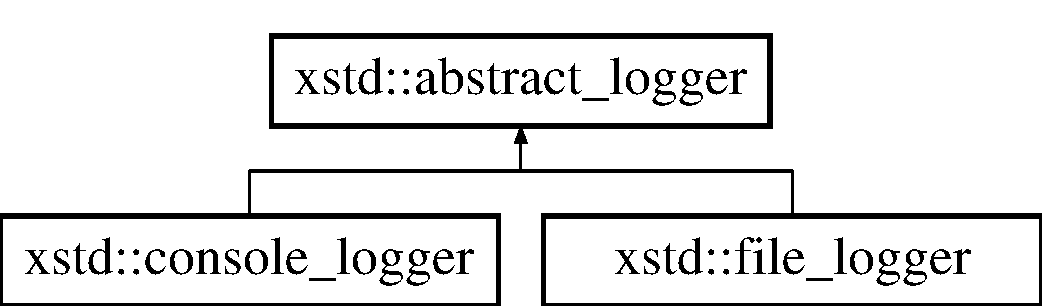
\includegraphics[height=2.000000cm]{classxstd_1_1abstract__logger}
\end{center}
\end{figure}
\subsection*{Public Member Functions}
\begin{DoxyCompactItemize}
\item 
\hypertarget{classxstd_1_1abstract__logger_a57d17bcf4d3260fab819d98643671c78}{{\bfseries abstract\-\_\-logger} (bool add\-\_\-new\-\_\-line=true, bool add\-\_\-time\-\_\-stamp=true) noexcept}\label{classxstd_1_1abstract__logger_a57d17bcf4d3260fab819d98643671c78}

\item 
\hypertarget{classxstd_1_1abstract__logger_ad470970ac4726355f3423017f434ace8}{void {\bfseries log} (const std\-::string \&data) const noexcept}\label{classxstd_1_1abstract__logger_ad470970ac4726355f3423017f434ace8}

\end{DoxyCompactItemize}
\subsection*{Public Attributes}
\begin{DoxyCompactItemize}
\item 
\hypertarget{classxstd_1_1abstract__logger_a5216ec0a18fea2571db19d5a55d8700f}{bool {\bfseries add\-\_\-new\-\_\-line}}\label{classxstd_1_1abstract__logger_a5216ec0a18fea2571db19d5a55d8700f}

\item 
\hypertarget{classxstd_1_1abstract__logger_a534b4f6a3dcdd3b7f18abfcb1bb5b937}{bool {\bfseries add\-\_\-time\-\_\-stamp}}\label{classxstd_1_1abstract__logger_a534b4f6a3dcdd3b7f18abfcb1bb5b937}

\end{DoxyCompactItemize}
\subsection*{Protected Member Functions}
\begin{DoxyCompactItemize}
\item 
\hypertarget{classxstd_1_1abstract__logger_a8cf4f5fd1490b54680060022a2f8ac91}{virtual void {\bfseries log\-\_\-data} (const std\-::string \&data) const noexcept=0}\label{classxstd_1_1abstract__logger_a8cf4f5fd1490b54680060022a2f8ac91}

\item 
\hypertarget{classxstd_1_1abstract__logger_a106b39652dd0d1efb32d8ad52ae6555c}{void {\bfseries log\-\_\-new\-\_\-line} (void) const noexcept}\label{classxstd_1_1abstract__logger_a106b39652dd0d1efb32d8ad52ae6555c}

\item 
\hypertarget{classxstd_1_1abstract__logger_a8bed4dfa79399f58146700adfd1ac06f}{void {\bfseries log\-\_\-time\-\_\-stamp} (void) const noexcept}\label{classxstd_1_1abstract__logger_a8bed4dfa79399f58146700adfd1ac06f}

\end{DoxyCompactItemize}
\subsection*{Static Protected Member Functions}
\begin{DoxyCompactItemize}
\item 
\hypertarget{classxstd_1_1abstract__logger_a1077a739173ed39b8f71f0ef69ada29f}{static std\-::string {\bfseries make\-\_\-time\-\_\-stamp} (void) noexcept}\label{classxstd_1_1abstract__logger_a1077a739173ed39b8f71f0ef69ada29f}

\end{DoxyCompactItemize}


The documentation for this class was generated from the following files\-:\begin{DoxyCompactItemize}
\item 
src/log/abstract\-\_\-logger/src/abstract\-\_\-logger.\-hpp\item 
src/log/abstract\-\_\-logger/src/abstract\-\_\-logger.\-ipp\end{DoxyCompactItemize}

\hypertarget{classxstd_1_1console__logger}{\section{xstd\-:\-:console\-\_\-logger Class Reference}
\label{classxstd_1_1console__logger}\index{xstd\-::console\-\_\-logger@{xstd\-::console\-\_\-logger}}
}


{\ttfamily \#include $<$console\-\_\-logger.\-hpp$>$}

Inheritance diagram for xstd\-:\-:console\-\_\-logger\-:\begin{figure}[H]
\begin{center}
\leavevmode
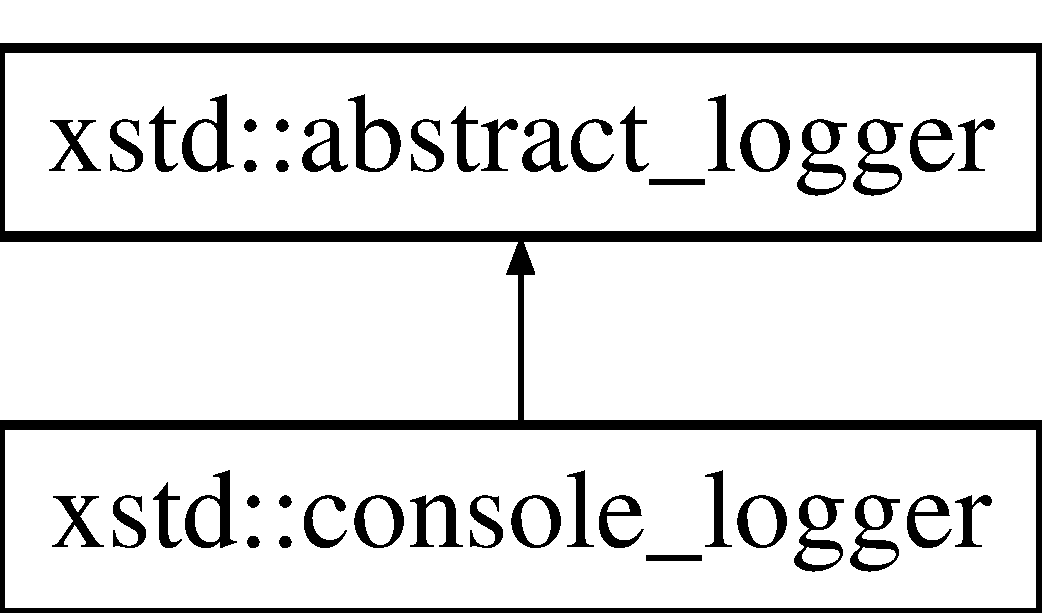
\includegraphics[height=2.000000cm]{classxstd_1_1console__logger}
\end{center}
\end{figure}
\subsection*{Public Member Functions}
\begin{DoxyCompactItemize}
\item 
\hyperlink{classxstd_1_1console__logger_a81ece8d9559e0ff0d54ad8d6cca596bc}{console\-\_\-logger} (bool \hyperlink{classxstd_1_1abstract__logger_a5216ec0a18fea2571db19d5a55d8700f}{add\-\_\-new\-\_\-line}=true, bool \hyperlink{classxstd_1_1abstract__logger_a534b4f6a3dcdd3b7f18abfcb1bb5b937}{add\-\_\-time\-\_\-stamp}=true) noexcept
\item 
void \hyperlink{classxstd_1_1abstract__logger_ad470970ac4726355f3423017f434ace8}{log} (const std\-::string \&data) const noexcept
\end{DoxyCompactItemize}
\subsection*{Public Attributes}
\begin{DoxyCompactItemize}
\item 
bool \hyperlink{classxstd_1_1abstract__logger_a5216ec0a18fea2571db19d5a55d8700f}{add\-\_\-new\-\_\-line}
\item 
bool \hyperlink{classxstd_1_1abstract__logger_a534b4f6a3dcdd3b7f18abfcb1bb5b937}{add\-\_\-time\-\_\-stamp}
\end{DoxyCompactItemize}
\subsection*{Protected Member Functions}
\begin{DoxyCompactItemize}
\item 
virtual void \hyperlink{classxstd_1_1console__logger_ad53afba0752b8cca7e5ccde101ec0954}{log\-\_\-data} (const std\-::string \&data) const noexcept override
\item 
void \hyperlink{classxstd_1_1abstract__logger_a106b39652dd0d1efb32d8ad52ae6555c}{log\-\_\-new\-\_\-line} (void) const noexcept
\item 
void \hyperlink{classxstd_1_1abstract__logger_a8bed4dfa79399f58146700adfd1ac06f}{log\-\_\-time\-\_\-stamp} (void) const noexcept
\end{DoxyCompactItemize}
\subsection*{Static Protected Member Functions}
\begin{DoxyCompactItemize}
\item 
static std\-::string \hyperlink{classxstd_1_1abstract__logger_a1077a739173ed39b8f71f0ef69ada29f}{make\-\_\-time\-\_\-stamp} (void) noexcept
\end{DoxyCompactItemize}


\subsection{Constructor \& Destructor Documentation}
\hypertarget{classxstd_1_1console__logger_a81ece8d9559e0ff0d54ad8d6cca596bc}{\index{xstd\-::console\-\_\-logger@{xstd\-::console\-\_\-logger}!console\-\_\-logger@{console\-\_\-logger}}
\index{console\-\_\-logger@{console\-\_\-logger}!xstd::console_logger@{xstd\-::console\-\_\-logger}}
\subsubsection[{console\-\_\-logger}]{\setlength{\rightskip}{0pt plus 5cm}xstd\-::console\-\_\-logger\-::console\-\_\-logger (
\begin{DoxyParamCaption}
\item[{bool}]{add\-\_\-new\-\_\-line = {\ttfamily true}, }
\item[{bool}]{add\-\_\-time\-\_\-stamp = {\ttfamily true}}
\end{DoxyParamCaption}
)\hspace{0.3cm}{\ttfamily [inline]}, {\ttfamily [explicit]}}}\label{classxstd_1_1console__logger_a81ece8d9559e0ff0d54ad8d6cca596bc}


\subsection{Member Function Documentation}
\hypertarget{classxstd_1_1abstract__logger_ad470970ac4726355f3423017f434ace8}{\index{xstd\-::console\-\_\-logger@{xstd\-::console\-\_\-logger}!log@{log}}
\index{log@{log}!xstd::console_logger@{xstd\-::console\-\_\-logger}}
\subsubsection[{log}]{\setlength{\rightskip}{0pt plus 5cm}void xstd\-::abstract\-\_\-logger\-::log (
\begin{DoxyParamCaption}
\item[{const std\-::string \&}]{data}
\end{DoxyParamCaption}
) const\hspace{0.3cm}{\ttfamily [inline]}, {\ttfamily [inherited]}}}\label{classxstd_1_1abstract__logger_ad470970ac4726355f3423017f434ace8}
\hypertarget{classxstd_1_1console__logger_ad53afba0752b8cca7e5ccde101ec0954}{\index{xstd\-::console\-\_\-logger@{xstd\-::console\-\_\-logger}!log\-\_\-data@{log\-\_\-data}}
\index{log\-\_\-data@{log\-\_\-data}!xstd::console_logger@{xstd\-::console\-\_\-logger}}
\subsubsection[{log\-\_\-data}]{\setlength{\rightskip}{0pt plus 5cm}void xstd\-::console\-\_\-logger\-::log\-\_\-data (
\begin{DoxyParamCaption}
\item[{const std\-::string \&}]{data}
\end{DoxyParamCaption}
) const\hspace{0.3cm}{\ttfamily [inline]}, {\ttfamily [override]}, {\ttfamily [protected]}, {\ttfamily [virtual]}}}\label{classxstd_1_1console__logger_ad53afba0752b8cca7e5ccde101ec0954}


Implements \hyperlink{classxstd_1_1abstract__logger_a8cf4f5fd1490b54680060022a2f8ac91}{xstd\-::abstract\-\_\-logger}.

\hypertarget{classxstd_1_1abstract__logger_a106b39652dd0d1efb32d8ad52ae6555c}{\index{xstd\-::console\-\_\-logger@{xstd\-::console\-\_\-logger}!log\-\_\-new\-\_\-line@{log\-\_\-new\-\_\-line}}
\index{log\-\_\-new\-\_\-line@{log\-\_\-new\-\_\-line}!xstd::console_logger@{xstd\-::console\-\_\-logger}}
\subsubsection[{log\-\_\-new\-\_\-line}]{\setlength{\rightskip}{0pt plus 5cm}void xstd\-::abstract\-\_\-logger\-::log\-\_\-new\-\_\-line (
\begin{DoxyParamCaption}
\item[{void}]{}
\end{DoxyParamCaption}
) const\hspace{0.3cm}{\ttfamily [inline]}, {\ttfamily [protected]}, {\ttfamily [inherited]}}}\label{classxstd_1_1abstract__logger_a106b39652dd0d1efb32d8ad52ae6555c}
\hypertarget{classxstd_1_1abstract__logger_a8bed4dfa79399f58146700adfd1ac06f}{\index{xstd\-::console\-\_\-logger@{xstd\-::console\-\_\-logger}!log\-\_\-time\-\_\-stamp@{log\-\_\-time\-\_\-stamp}}
\index{log\-\_\-time\-\_\-stamp@{log\-\_\-time\-\_\-stamp}!xstd::console_logger@{xstd\-::console\-\_\-logger}}
\subsubsection[{log\-\_\-time\-\_\-stamp}]{\setlength{\rightskip}{0pt plus 5cm}void xstd\-::abstract\-\_\-logger\-::log\-\_\-time\-\_\-stamp (
\begin{DoxyParamCaption}
\item[{void}]{}
\end{DoxyParamCaption}
) const\hspace{0.3cm}{\ttfamily [inline]}, {\ttfamily [protected]}, {\ttfamily [inherited]}}}\label{classxstd_1_1abstract__logger_a8bed4dfa79399f58146700adfd1ac06f}
\hypertarget{classxstd_1_1abstract__logger_a1077a739173ed39b8f71f0ef69ada29f}{\index{xstd\-::console\-\_\-logger@{xstd\-::console\-\_\-logger}!make\-\_\-time\-\_\-stamp@{make\-\_\-time\-\_\-stamp}}
\index{make\-\_\-time\-\_\-stamp@{make\-\_\-time\-\_\-stamp}!xstd::console_logger@{xstd\-::console\-\_\-logger}}
\subsubsection[{make\-\_\-time\-\_\-stamp}]{\setlength{\rightskip}{0pt plus 5cm}std\-::string xstd\-::abstract\-\_\-logger\-::make\-\_\-time\-\_\-stamp (
\begin{DoxyParamCaption}
\item[{void}]{}
\end{DoxyParamCaption}
)\hspace{0.3cm}{\ttfamily [inline]}, {\ttfamily [static]}, {\ttfamily [protected]}, {\ttfamily [inherited]}}}\label{classxstd_1_1abstract__logger_a1077a739173ed39b8f71f0ef69ada29f}


\subsection{Member Data Documentation}
\hypertarget{classxstd_1_1abstract__logger_a5216ec0a18fea2571db19d5a55d8700f}{\index{xstd\-::console\-\_\-logger@{xstd\-::console\-\_\-logger}!add\-\_\-new\-\_\-line@{add\-\_\-new\-\_\-line}}
\index{add\-\_\-new\-\_\-line@{add\-\_\-new\-\_\-line}!xstd::console_logger@{xstd\-::console\-\_\-logger}}
\subsubsection[{add\-\_\-new\-\_\-line}]{\setlength{\rightskip}{0pt plus 5cm}bool xstd\-::abstract\-\_\-logger\-::add\-\_\-new\-\_\-line\hspace{0.3cm}{\ttfamily [inherited]}}}\label{classxstd_1_1abstract__logger_a5216ec0a18fea2571db19d5a55d8700f}
\hypertarget{classxstd_1_1abstract__logger_a534b4f6a3dcdd3b7f18abfcb1bb5b937}{\index{xstd\-::console\-\_\-logger@{xstd\-::console\-\_\-logger}!add\-\_\-time\-\_\-stamp@{add\-\_\-time\-\_\-stamp}}
\index{add\-\_\-time\-\_\-stamp@{add\-\_\-time\-\_\-stamp}!xstd::console_logger@{xstd\-::console\-\_\-logger}}
\subsubsection[{add\-\_\-time\-\_\-stamp}]{\setlength{\rightskip}{0pt plus 5cm}bool xstd\-::abstract\-\_\-logger\-::add\-\_\-time\-\_\-stamp\hspace{0.3cm}{\ttfamily [inherited]}}}\label{classxstd_1_1abstract__logger_a534b4f6a3dcdd3b7f18abfcb1bb5b937}


The documentation for this class was generated from the following files\-:\begin{DoxyCompactItemize}
\item 
src/log/console\-\_\-logger/src/\hyperlink{console__logger_8hpp}{console\-\_\-logger.\-hpp}\item 
src/log/console\-\_\-logger/src/\hyperlink{console__logger_8ipp}{console\-\_\-logger.\-ipp}\end{DoxyCompactItemize}

\hypertarget{classxstd_1_1coutmt__singleton}{\section{xstd\-:\-:coutmt\-\_\-singleton Class Reference}
\label{classxstd_1_1coutmt__singleton}\index{xstd\-::coutmt\-\_\-singleton@{xstd\-::coutmt\-\_\-singleton}}
}
\subsection*{Static Public Member Functions}
\begin{DoxyCompactItemize}
\item 
\hypertarget{classxstd_1_1coutmt__singleton_a0c478170b82e253a79c51160fe7049a2}{static \hyperlink{classxstd_1_1coutmt__singleton}{coutmt\-\_\-singleton} \& {\bfseries get\-\_\-instance} (void)}\label{classxstd_1_1coutmt__singleton_a0c478170b82e253a79c51160fe7049a2}

\end{DoxyCompactItemize}
\subsection*{Friends}
\begin{DoxyCompactItemize}
\item 
\hypertarget{classxstd_1_1coutmt__singleton_aae5812b8fa2d66eaaa921e864e1077d4}{{\footnotesize template$<$typename Type $>$ }\\\hyperlink{classxstd_1_1coutmt__singleton}{coutmt\-\_\-singleton} \& {\bfseries operator$<$$<$} (\hyperlink{classxstd_1_1coutmt__singleton}{coutmt\-\_\-singleton} \&coutmt\-\_\-singleton\-\_\-instance, Type object)}\label{classxstd_1_1coutmt__singleton_aae5812b8fa2d66eaaa921e864e1077d4}

\item 
\hypertarget{classxstd_1_1coutmt__singleton_a75138493a4c47f61c28762df29d5af97}{\hyperlink{classxstd_1_1coutmt__singleton}{coutmt\-\_\-singleton} \& {\bfseries operator$<$$<$} (\hyperlink{classxstd_1_1coutmt__singleton}{coutmt\-\_\-singleton} \&coutmt\-\_\-singleton\-\_\-instance, std\-::ostream \&($\ast$function\-\_\-ptr)(std\-::ostream \&))}\label{classxstd_1_1coutmt__singleton_a75138493a4c47f61c28762df29d5af97}

\item 
\hypertarget{classxstd_1_1coutmt__singleton_af343264ff6f5ba75b8f6eab378c55638}{\hyperlink{classxstd_1_1coutmt__singleton}{coutmt\-\_\-singleton} \& {\bfseries operator$<$$<$} (\hyperlink{classxstd_1_1coutmt__singleton}{coutmt\-\_\-singleton} \&coutmt\-\_\-singleton\-\_\-instance, std\-::ios \&($\ast$function\-\_\-ptr)(std\-::ios \&))}\label{classxstd_1_1coutmt__singleton_af343264ff6f5ba75b8f6eab378c55638}

\item 
\hypertarget{classxstd_1_1coutmt__singleton_af794d8d7f2993af42e84429e5f5b4c9a}{\hyperlink{classxstd_1_1coutmt__singleton}{coutmt\-\_\-singleton} \& {\bfseries operator$<$$<$} (\hyperlink{classxstd_1_1coutmt__singleton}{coutmt\-\_\-singleton} \&coutmt\-\_\-singleton\-\_\-instance, std\-::ios\-\_\-base \&($\ast$function\-\_\-ptr)(std\-::ios\-\_\-base \&))}\label{classxstd_1_1coutmt__singleton_af794d8d7f2993af42e84429e5f5b4c9a}

\end{DoxyCompactItemize}


The documentation for this class was generated from the following files\-:\begin{DoxyCompactItemize}
\item 
src/iostream/coutmt/src/coutmt.\-hpp\item 
src/iostream/coutmt/src/coutmt.\-ipp\end{DoxyCompactItemize}

\hypertarget{structxstd_1_1dimension__mismatch}{\section{xstd\-:\-:dimension\-\_\-mismatch Struct Reference}
\label{structxstd_1_1dimension__mismatch}\index{xstd\-::dimension\-\_\-mismatch@{xstd\-::dimension\-\_\-mismatch}}
}


{\ttfamily \#include $<$point.\-hpp$>$}



The documentation for this struct was generated from the following file\-:\begin{DoxyCompactItemize}
\item 
src/cmath/point/src/\hyperlink{point_8hpp}{point.\-hpp}\end{DoxyCompactItemize}

\hypertarget{classxstd_1_1event}{\section{xstd\-:\-:event$<$ data\-\_\-type $>$ Class Template Reference}
\label{classxstd_1_1event}\index{xstd\-::event$<$ data\-\_\-type $>$@{xstd\-::event$<$ data\-\_\-type $>$}}
}


{\ttfamily \#include $<$event.\-hpp$>$}

\subsection*{Public Member Functions}
\begin{DoxyCompactItemize}
\item 
virtual \hyperlink{classxstd_1_1event_a5818ac871d63b38a5409eb3b153c3bef}{$\sim$event} (void) noexcept
\item 
unsigned int \hyperlink{classxstd_1_1event_af5ce6caa7da361833c3098686a28eb4a}{get\-\_\-listeners\-\_\-count} (void) const 
\item 
unsigned int \hyperlink{classxstd_1_1event_a91e77f734b2fe690615a9684446594a9}{get\-\_\-free\-\_\-listeners\-\_\-count} (void) const 
\item 
unsigned int \hyperlink{classxstd_1_1event_a6aec13f27635f3ad58435337f6063659}{get\-\_\-functor\-\_\-listeners\-\_\-count} (void) const 
\item 
bool \hyperlink{classxstd_1_1event_a28d29a9104d4e8c3986376b2ffca0a48}{has\-\_\-listener} (free\-\_\-listener free\-\_\-listener\-\_\-instance) const 
\item 
{\footnotesize template$<$typename object\-\_\-type $>$ }\\bool \hyperlink{classxstd_1_1event_acbfdc5b60687237a2b42bc6e7d00d4a4}{has\-\_\-listener} (object\-\_\-type $\ast$object\-\_\-ptr, void(object\-\_\-type\-::$\ast$method\-\_\-ptr)(data\-\_\-type...)) const 
\item 
void \hyperlink{classxstd_1_1event_a6d7320f608d4f7b072b62a5e66ea8d62}{add\-\_\-listener} (free\-\_\-listener free\-\_\-listener\-\_\-instance)
\item 
{\footnotesize template$<$typename object\-\_\-type $>$ }\\void \hyperlink{classxstd_1_1event_aa58880f86e0e2e5653df91692f221604}{add\-\_\-listener} (object\-\_\-type $\ast$object\-\_\-ptr, void(object\-\_\-type\-::$\ast$method\-\_\-ptr)(data\-\_\-type...))
\item 
void \hyperlink{classxstd_1_1event_a19e40e6d6af2d565ef741ecfbfb2fda7}{remove\-\_\-listener} (free\-\_\-listener free\-\_\-listener\-\_\-instance)
\item 
{\footnotesize template$<$typename object\-\_\-type $>$ }\\void \hyperlink{classxstd_1_1event_a2ecf3e9a39708db0c28281dbb32d12da}{remove\-\_\-listener} (object\-\_\-type $\ast$object\-\_\-ptr, void(object\-\_\-type\-::$\ast$method\-\_\-ptr)(data\-\_\-type...))
\item 
void \hyperlink{classxstd_1_1event_a60e1b1471f7c50f764fcb8388ca56b47}{dispatch} (data\-\_\-type...\-data) const 
\end{DoxyCompactItemize}
\subsection*{Protected Member Functions}
\begin{DoxyCompactItemize}
\item 
void \hyperlink{classxstd_1_1event_a3b2ec0fe63b51f0a785663ff1cbaf897}{check\-\_\-has\-\_\-listener} (free\-\_\-listener free\-\_\-listener\-\_\-instance) const 
\item 
{\footnotesize template$<$typename object\-\_\-type $>$ }\\void \hyperlink{classxstd_1_1event_a4c8f61670b0145de08594411dab17b49}{check\-\_\-has\-\_\-listener} (object\-\_\-type $\ast$object\-\_\-ptr, void(object\-\_\-type\-::$\ast$method\-\_\-ptr)(data\-\_\-type...)) const 
\item 
void \hyperlink{classxstd_1_1event_a8720bdcd9e0e8588eadbca2750f751e0}{check\-\_\-has\-\_\-no\-\_\-listener} (free\-\_\-listener free\-\_\-listener\-\_\-instance) const 
\item 
{\footnotesize template$<$typename object\-\_\-type $>$ }\\void \hyperlink{classxstd_1_1event_a38563e182cb13274550c790f6c2d48e1}{check\-\_\-has\-\_\-no\-\_\-listener} (object\-\_\-type $\ast$object\-\_\-ptr, void(object\-\_\-type\-::$\ast$method\-\_\-ptr)(data\-\_\-type...)) const 
\item 
free\-\_\-listeners\-\_\-collection\-\_\-itr \hyperlink{classxstd_1_1event_ac5c004598aa8803f901597ade5aec2c2}{get\-\_\-listener\-\_\-itr} (free\-\_\-listener free\-\_\-listener\-\_\-instance) const 
\item 
{\footnotesize template$<$typename object\-\_\-type $>$ }\\functor\-\_\-listeners\-\_\-collection\-\_\-itr \hyperlink{classxstd_1_1event_a56491edd13a1c81766c8c770464e992a}{get\-\_\-listener\-\_\-itr} (object\-\_\-type $\ast$object\-\_\-ptr, void(object\-\_\-type\-::$\ast$method\-\_\-ptr)(data\-\_\-type...)) const 
\item 
void \hyperlink{classxstd_1_1event_ac3a4cf6f6d139f3ab31cd3ca1ebb42e0}{dispatch\-\_\-free\-\_\-listeners} (data\-\_\-type...\-data) const 
\item 
void \hyperlink{classxstd_1_1event_a3c82e7e9e05c4c44e65b32db7090bd3c}{dispatch\-\_\-functor\-\_\-listeners} (data\-\_\-type...\-data) const 
\end{DoxyCompactItemize}
\subsection*{Protected Attributes}
\begin{DoxyCompactItemize}
\item 
free\-\_\-listeners\-\_\-collection \hyperlink{classxstd_1_1event_a045873dfdf4fe07af8421d81592d3275}{free\-\_\-listeners}
\item 
functor\-\_\-listeners\-\_\-collection \hyperlink{classxstd_1_1event_a3e4c0ca4abd96a0af619cdb96e3cfef2}{functor\-\_\-listeners}
\item 
std\-::recursive\-\_\-mutex \hyperlink{classxstd_1_1event_afaaee3e44989122c9e1db6f4d1547de8}{master\-\_\-mutex}
\end{DoxyCompactItemize}


\subsection{Constructor \& Destructor Documentation}
\hypertarget{classxstd_1_1event_a5818ac871d63b38a5409eb3b153c3bef}{\index{xstd\-::event@{xstd\-::event}!$\sim$event@{$\sim$event}}
\index{$\sim$event@{$\sim$event}!xstd::event@{xstd\-::event}}
\subsubsection[{$\sim$event}]{\setlength{\rightskip}{0pt plus 5cm}template$<$typename... data\-\_\-type$>$ virtual {\bf xstd\-::event}$<$ data\-\_\-type $>$\-::$\sim${\bf event} (
\begin{DoxyParamCaption}
\item[{void}]{}
\end{DoxyParamCaption}
)\hspace{0.3cm}{\ttfamily [inline]}, {\ttfamily [virtual]}}}\label{classxstd_1_1event_a5818ac871d63b38a5409eb3b153c3bef}


\subsection{Member Function Documentation}
\hypertarget{classxstd_1_1event_a6d7320f608d4f7b072b62a5e66ea8d62}{\index{xstd\-::event@{xstd\-::event}!add\-\_\-listener@{add\-\_\-listener}}
\index{add\-\_\-listener@{add\-\_\-listener}!xstd::event@{xstd\-::event}}
\subsubsection[{add\-\_\-listener}]{\setlength{\rightskip}{0pt plus 5cm}template$<$typename... data\-\_\-type$>$ void {\bf xstd\-::event}$<$ data\-\_\-type $>$\-::add\-\_\-listener (
\begin{DoxyParamCaption}
\item[{free\-\_\-listener}]{free\-\_\-listener\-\_\-instance}
\end{DoxyParamCaption}
)\hspace{0.3cm}{\ttfamily [inline]}}}\label{classxstd_1_1event_a6d7320f608d4f7b072b62a5e66ea8d62}
\hypertarget{classxstd_1_1event_aa58880f86e0e2e5653df91692f221604}{\index{xstd\-::event@{xstd\-::event}!add\-\_\-listener@{add\-\_\-listener}}
\index{add\-\_\-listener@{add\-\_\-listener}!xstd::event@{xstd\-::event}}
\subsubsection[{add\-\_\-listener}]{\setlength{\rightskip}{0pt plus 5cm}template$<$typename... data\-\_\-type$>$ template$<$typename object\-\_\-type $>$ void {\bf xstd\-::event}$<$ data\-\_\-type $>$\-::add\-\_\-listener (
\begin{DoxyParamCaption}
\item[{object\-\_\-type $\ast$}]{object\-\_\-ptr, }
\item[{void(object\-\_\-type\-::$\ast$)(data\-\_\-type...)}]{method\-\_\-ptr}
\end{DoxyParamCaption}
)\hspace{0.3cm}{\ttfamily [inline]}}}\label{classxstd_1_1event_aa58880f86e0e2e5653df91692f221604}
\hypertarget{classxstd_1_1event_a3b2ec0fe63b51f0a785663ff1cbaf897}{\index{xstd\-::event@{xstd\-::event}!check\-\_\-has\-\_\-listener@{check\-\_\-has\-\_\-listener}}
\index{check\-\_\-has\-\_\-listener@{check\-\_\-has\-\_\-listener}!xstd::event@{xstd\-::event}}
\subsubsection[{check\-\_\-has\-\_\-listener}]{\setlength{\rightskip}{0pt plus 5cm}template$<$typename... data\-\_\-type$>$ void {\bf xstd\-::event}$<$ data\-\_\-type $>$\-::check\-\_\-has\-\_\-listener (
\begin{DoxyParamCaption}
\item[{free\-\_\-listener}]{free\-\_\-listener\-\_\-instance}
\end{DoxyParamCaption}
) const\hspace{0.3cm}{\ttfamily [inline]}, {\ttfamily [protected]}}}\label{classxstd_1_1event_a3b2ec0fe63b51f0a785663ff1cbaf897}
\hypertarget{classxstd_1_1event_a4c8f61670b0145de08594411dab17b49}{\index{xstd\-::event@{xstd\-::event}!check\-\_\-has\-\_\-listener@{check\-\_\-has\-\_\-listener}}
\index{check\-\_\-has\-\_\-listener@{check\-\_\-has\-\_\-listener}!xstd::event@{xstd\-::event}}
\subsubsection[{check\-\_\-has\-\_\-listener}]{\setlength{\rightskip}{0pt plus 5cm}template$<$typename... data\-\_\-type$>$ template$<$typename object\-\_\-type $>$ void {\bf xstd\-::event}$<$ data\-\_\-type $>$\-::check\-\_\-has\-\_\-listener (
\begin{DoxyParamCaption}
\item[{object\-\_\-type $\ast$}]{object\-\_\-ptr, }
\item[{void(object\-\_\-type\-::$\ast$)(data\-\_\-type...)}]{method\-\_\-ptr}
\end{DoxyParamCaption}
) const\hspace{0.3cm}{\ttfamily [inline]}, {\ttfamily [protected]}}}\label{classxstd_1_1event_a4c8f61670b0145de08594411dab17b49}
\hypertarget{classxstd_1_1event_a8720bdcd9e0e8588eadbca2750f751e0}{\index{xstd\-::event@{xstd\-::event}!check\-\_\-has\-\_\-no\-\_\-listener@{check\-\_\-has\-\_\-no\-\_\-listener}}
\index{check\-\_\-has\-\_\-no\-\_\-listener@{check\-\_\-has\-\_\-no\-\_\-listener}!xstd::event@{xstd\-::event}}
\subsubsection[{check\-\_\-has\-\_\-no\-\_\-listener}]{\setlength{\rightskip}{0pt plus 5cm}template$<$typename... data\-\_\-type$>$ void {\bf xstd\-::event}$<$ data\-\_\-type $>$\-::check\-\_\-has\-\_\-no\-\_\-listener (
\begin{DoxyParamCaption}
\item[{free\-\_\-listener}]{free\-\_\-listener\-\_\-instance}
\end{DoxyParamCaption}
) const\hspace{0.3cm}{\ttfamily [inline]}, {\ttfamily [protected]}}}\label{classxstd_1_1event_a8720bdcd9e0e8588eadbca2750f751e0}
\hypertarget{classxstd_1_1event_a38563e182cb13274550c790f6c2d48e1}{\index{xstd\-::event@{xstd\-::event}!check\-\_\-has\-\_\-no\-\_\-listener@{check\-\_\-has\-\_\-no\-\_\-listener}}
\index{check\-\_\-has\-\_\-no\-\_\-listener@{check\-\_\-has\-\_\-no\-\_\-listener}!xstd::event@{xstd\-::event}}
\subsubsection[{check\-\_\-has\-\_\-no\-\_\-listener}]{\setlength{\rightskip}{0pt plus 5cm}template$<$typename... data\-\_\-type$>$ template$<$typename object\-\_\-type $>$ void {\bf xstd\-::event}$<$ data\-\_\-type $>$\-::check\-\_\-has\-\_\-no\-\_\-listener (
\begin{DoxyParamCaption}
\item[{object\-\_\-type $\ast$}]{object\-\_\-ptr, }
\item[{void(object\-\_\-type\-::$\ast$)(data\-\_\-type...)}]{method\-\_\-ptr}
\end{DoxyParamCaption}
) const\hspace{0.3cm}{\ttfamily [inline]}, {\ttfamily [protected]}}}\label{classxstd_1_1event_a38563e182cb13274550c790f6c2d48e1}
\hypertarget{classxstd_1_1event_a60e1b1471f7c50f764fcb8388ca56b47}{\index{xstd\-::event@{xstd\-::event}!dispatch@{dispatch}}
\index{dispatch@{dispatch}!xstd::event@{xstd\-::event}}
\subsubsection[{dispatch}]{\setlength{\rightskip}{0pt plus 5cm}template$<$typename... data\-\_\-type$>$ void {\bf xstd\-::event}$<$ data\-\_\-type $>$\-::dispatch (
\begin{DoxyParamCaption}
\item[{data\-\_\-type...}]{data}
\end{DoxyParamCaption}
) const\hspace{0.3cm}{\ttfamily [inline]}}}\label{classxstd_1_1event_a60e1b1471f7c50f764fcb8388ca56b47}
\hypertarget{classxstd_1_1event_ac3a4cf6f6d139f3ab31cd3ca1ebb42e0}{\index{xstd\-::event@{xstd\-::event}!dispatch\-\_\-free\-\_\-listeners@{dispatch\-\_\-free\-\_\-listeners}}
\index{dispatch\-\_\-free\-\_\-listeners@{dispatch\-\_\-free\-\_\-listeners}!xstd::event@{xstd\-::event}}
\subsubsection[{dispatch\-\_\-free\-\_\-listeners}]{\setlength{\rightskip}{0pt plus 5cm}template$<$typename... data\-\_\-type$>$ void {\bf xstd\-::event}$<$ data\-\_\-type $>$\-::dispatch\-\_\-free\-\_\-listeners (
\begin{DoxyParamCaption}
\item[{data\-\_\-type...}]{data}
\end{DoxyParamCaption}
) const\hspace{0.3cm}{\ttfamily [inline]}, {\ttfamily [protected]}}}\label{classxstd_1_1event_ac3a4cf6f6d139f3ab31cd3ca1ebb42e0}
\hypertarget{classxstd_1_1event_a3c82e7e9e05c4c44e65b32db7090bd3c}{\index{xstd\-::event@{xstd\-::event}!dispatch\-\_\-functor\-\_\-listeners@{dispatch\-\_\-functor\-\_\-listeners}}
\index{dispatch\-\_\-functor\-\_\-listeners@{dispatch\-\_\-functor\-\_\-listeners}!xstd::event@{xstd\-::event}}
\subsubsection[{dispatch\-\_\-functor\-\_\-listeners}]{\setlength{\rightskip}{0pt plus 5cm}template$<$typename... data\-\_\-type$>$ void {\bf xstd\-::event}$<$ data\-\_\-type $>$\-::dispatch\-\_\-functor\-\_\-listeners (
\begin{DoxyParamCaption}
\item[{data\-\_\-type...}]{data}
\end{DoxyParamCaption}
) const\hspace{0.3cm}{\ttfamily [inline]}, {\ttfamily [protected]}}}\label{classxstd_1_1event_a3c82e7e9e05c4c44e65b32db7090bd3c}
\hypertarget{classxstd_1_1event_a91e77f734b2fe690615a9684446594a9}{\index{xstd\-::event@{xstd\-::event}!get\-\_\-free\-\_\-listeners\-\_\-count@{get\-\_\-free\-\_\-listeners\-\_\-count}}
\index{get\-\_\-free\-\_\-listeners\-\_\-count@{get\-\_\-free\-\_\-listeners\-\_\-count}!xstd::event@{xstd\-::event}}
\subsubsection[{get\-\_\-free\-\_\-listeners\-\_\-count}]{\setlength{\rightskip}{0pt plus 5cm}template$<$typename... data\-\_\-type$>$ unsigned int {\bf xstd\-::event}$<$ data\-\_\-type $>$\-::get\-\_\-free\-\_\-listeners\-\_\-count (
\begin{DoxyParamCaption}
\item[{void}]{}
\end{DoxyParamCaption}
) const\hspace{0.3cm}{\ttfamily [inline]}}}\label{classxstd_1_1event_a91e77f734b2fe690615a9684446594a9}
\hypertarget{classxstd_1_1event_a6aec13f27635f3ad58435337f6063659}{\index{xstd\-::event@{xstd\-::event}!get\-\_\-functor\-\_\-listeners\-\_\-count@{get\-\_\-functor\-\_\-listeners\-\_\-count}}
\index{get\-\_\-functor\-\_\-listeners\-\_\-count@{get\-\_\-functor\-\_\-listeners\-\_\-count}!xstd::event@{xstd\-::event}}
\subsubsection[{get\-\_\-functor\-\_\-listeners\-\_\-count}]{\setlength{\rightskip}{0pt plus 5cm}template$<$typename... data\-\_\-type$>$ unsigned int {\bf xstd\-::event}$<$ data\-\_\-type $>$\-::get\-\_\-functor\-\_\-listeners\-\_\-count (
\begin{DoxyParamCaption}
\item[{void}]{}
\end{DoxyParamCaption}
) const\hspace{0.3cm}{\ttfamily [inline]}}}\label{classxstd_1_1event_a6aec13f27635f3ad58435337f6063659}
\hypertarget{classxstd_1_1event_ac5c004598aa8803f901597ade5aec2c2}{\index{xstd\-::event@{xstd\-::event}!get\-\_\-listener\-\_\-itr@{get\-\_\-listener\-\_\-itr}}
\index{get\-\_\-listener\-\_\-itr@{get\-\_\-listener\-\_\-itr}!xstd::event@{xstd\-::event}}
\subsubsection[{get\-\_\-listener\-\_\-itr}]{\setlength{\rightskip}{0pt plus 5cm}template$<$typename... data\-\_\-type$>$ free\-\_\-listeners\-\_\-collection\-\_\-itr {\bf xstd\-::event}$<$ data\-\_\-type $>$\-::get\-\_\-listener\-\_\-itr (
\begin{DoxyParamCaption}
\item[{free\-\_\-listener}]{free\-\_\-listener\-\_\-instance}
\end{DoxyParamCaption}
) const\hspace{0.3cm}{\ttfamily [inline]}, {\ttfamily [protected]}}}\label{classxstd_1_1event_ac5c004598aa8803f901597ade5aec2c2}
\hypertarget{classxstd_1_1event_a56491edd13a1c81766c8c770464e992a}{\index{xstd\-::event@{xstd\-::event}!get\-\_\-listener\-\_\-itr@{get\-\_\-listener\-\_\-itr}}
\index{get\-\_\-listener\-\_\-itr@{get\-\_\-listener\-\_\-itr}!xstd::event@{xstd\-::event}}
\subsubsection[{get\-\_\-listener\-\_\-itr}]{\setlength{\rightskip}{0pt plus 5cm}template$<$typename... data\-\_\-type$>$ template$<$typename object\-\_\-type $>$ functor\-\_\-listeners\-\_\-collection\-\_\-itr {\bf xstd\-::event}$<$ data\-\_\-type $>$\-::get\-\_\-listener\-\_\-itr (
\begin{DoxyParamCaption}
\item[{object\-\_\-type $\ast$}]{object\-\_\-ptr, }
\item[{void(object\-\_\-type\-::$\ast$)(data\-\_\-type...)}]{method\-\_\-ptr}
\end{DoxyParamCaption}
) const\hspace{0.3cm}{\ttfamily [inline]}, {\ttfamily [protected]}}}\label{classxstd_1_1event_a56491edd13a1c81766c8c770464e992a}
\hypertarget{classxstd_1_1event_af5ce6caa7da361833c3098686a28eb4a}{\index{xstd\-::event@{xstd\-::event}!get\-\_\-listeners\-\_\-count@{get\-\_\-listeners\-\_\-count}}
\index{get\-\_\-listeners\-\_\-count@{get\-\_\-listeners\-\_\-count}!xstd::event@{xstd\-::event}}
\subsubsection[{get\-\_\-listeners\-\_\-count}]{\setlength{\rightskip}{0pt plus 5cm}template$<$typename... data\-\_\-type$>$ unsigned int {\bf xstd\-::event}$<$ data\-\_\-type $>$\-::get\-\_\-listeners\-\_\-count (
\begin{DoxyParamCaption}
\item[{void}]{}
\end{DoxyParamCaption}
) const\hspace{0.3cm}{\ttfamily [inline]}}}\label{classxstd_1_1event_af5ce6caa7da361833c3098686a28eb4a}
\hypertarget{classxstd_1_1event_a28d29a9104d4e8c3986376b2ffca0a48}{\index{xstd\-::event@{xstd\-::event}!has\-\_\-listener@{has\-\_\-listener}}
\index{has\-\_\-listener@{has\-\_\-listener}!xstd::event@{xstd\-::event}}
\subsubsection[{has\-\_\-listener}]{\setlength{\rightskip}{0pt plus 5cm}template$<$typename... data\-\_\-type$>$ bool {\bf xstd\-::event}$<$ data\-\_\-type $>$\-::has\-\_\-listener (
\begin{DoxyParamCaption}
\item[{free\-\_\-listener}]{free\-\_\-listener\-\_\-instance}
\end{DoxyParamCaption}
) const\hspace{0.3cm}{\ttfamily [inline]}}}\label{classxstd_1_1event_a28d29a9104d4e8c3986376b2ffca0a48}
\hypertarget{classxstd_1_1event_acbfdc5b60687237a2b42bc6e7d00d4a4}{\index{xstd\-::event@{xstd\-::event}!has\-\_\-listener@{has\-\_\-listener}}
\index{has\-\_\-listener@{has\-\_\-listener}!xstd::event@{xstd\-::event}}
\subsubsection[{has\-\_\-listener}]{\setlength{\rightskip}{0pt plus 5cm}template$<$typename... data\-\_\-type$>$ template$<$typename object\-\_\-type $>$ bool {\bf xstd\-::event}$<$ data\-\_\-type $>$\-::has\-\_\-listener (
\begin{DoxyParamCaption}
\item[{object\-\_\-type $\ast$}]{object\-\_\-ptr, }
\item[{void(object\-\_\-type\-::$\ast$)(data\-\_\-type...)}]{method\-\_\-ptr}
\end{DoxyParamCaption}
) const\hspace{0.3cm}{\ttfamily [inline]}}}\label{classxstd_1_1event_acbfdc5b60687237a2b42bc6e7d00d4a4}
\hypertarget{classxstd_1_1event_a19e40e6d6af2d565ef741ecfbfb2fda7}{\index{xstd\-::event@{xstd\-::event}!remove\-\_\-listener@{remove\-\_\-listener}}
\index{remove\-\_\-listener@{remove\-\_\-listener}!xstd::event@{xstd\-::event}}
\subsubsection[{remove\-\_\-listener}]{\setlength{\rightskip}{0pt plus 5cm}template$<$typename... data\-\_\-type$>$ void {\bf xstd\-::event}$<$ data\-\_\-type $>$\-::remove\-\_\-listener (
\begin{DoxyParamCaption}
\item[{free\-\_\-listener}]{free\-\_\-listener\-\_\-instance}
\end{DoxyParamCaption}
)\hspace{0.3cm}{\ttfamily [inline]}}}\label{classxstd_1_1event_a19e40e6d6af2d565ef741ecfbfb2fda7}
\hypertarget{classxstd_1_1event_a2ecf3e9a39708db0c28281dbb32d12da}{\index{xstd\-::event@{xstd\-::event}!remove\-\_\-listener@{remove\-\_\-listener}}
\index{remove\-\_\-listener@{remove\-\_\-listener}!xstd::event@{xstd\-::event}}
\subsubsection[{remove\-\_\-listener}]{\setlength{\rightskip}{0pt plus 5cm}template$<$typename... data\-\_\-type$>$ template$<$typename object\-\_\-type $>$ void {\bf xstd\-::event}$<$ data\-\_\-type $>$\-::remove\-\_\-listener (
\begin{DoxyParamCaption}
\item[{object\-\_\-type $\ast$}]{object\-\_\-ptr, }
\item[{void(object\-\_\-type\-::$\ast$)(data\-\_\-type...)}]{method\-\_\-ptr}
\end{DoxyParamCaption}
)\hspace{0.3cm}{\ttfamily [inline]}}}\label{classxstd_1_1event_a2ecf3e9a39708db0c28281dbb32d12da}


\subsection{Member Data Documentation}
\hypertarget{classxstd_1_1event_a045873dfdf4fe07af8421d81592d3275}{\index{xstd\-::event@{xstd\-::event}!free\-\_\-listeners@{free\-\_\-listeners}}
\index{free\-\_\-listeners@{free\-\_\-listeners}!xstd::event@{xstd\-::event}}
\subsubsection[{free\-\_\-listeners}]{\setlength{\rightskip}{0pt plus 5cm}template$<$typename... data\-\_\-type$>$ free\-\_\-listeners\-\_\-collection {\bf xstd\-::event}$<$ data\-\_\-type $>$\-::free\-\_\-listeners\hspace{0.3cm}{\ttfamily [mutable]}, {\ttfamily [protected]}}}\label{classxstd_1_1event_a045873dfdf4fe07af8421d81592d3275}
\hypertarget{classxstd_1_1event_a3e4c0ca4abd96a0af619cdb96e3cfef2}{\index{xstd\-::event@{xstd\-::event}!functor\-\_\-listeners@{functor\-\_\-listeners}}
\index{functor\-\_\-listeners@{functor\-\_\-listeners}!xstd::event@{xstd\-::event}}
\subsubsection[{functor\-\_\-listeners}]{\setlength{\rightskip}{0pt plus 5cm}template$<$typename... data\-\_\-type$>$ functor\-\_\-listeners\-\_\-collection {\bf xstd\-::event}$<$ data\-\_\-type $>$\-::functor\-\_\-listeners\hspace{0.3cm}{\ttfamily [mutable]}, {\ttfamily [protected]}}}\label{classxstd_1_1event_a3e4c0ca4abd96a0af619cdb96e3cfef2}
\hypertarget{classxstd_1_1event_afaaee3e44989122c9e1db6f4d1547de8}{\index{xstd\-::event@{xstd\-::event}!master\-\_\-mutex@{master\-\_\-mutex}}
\index{master\-\_\-mutex@{master\-\_\-mutex}!xstd::event@{xstd\-::event}}
\subsubsection[{master\-\_\-mutex}]{\setlength{\rightskip}{0pt plus 5cm}template$<$typename... data\-\_\-type$>$ std\-::recursive\-\_\-mutex {\bf xstd\-::event}$<$ data\-\_\-type $>$\-::master\-\_\-mutex\hspace{0.3cm}{\ttfamily [mutable]}, {\ttfamily [protected]}}}\label{classxstd_1_1event_afaaee3e44989122c9e1db6f4d1547de8}


The documentation for this class was generated from the following file\-:\begin{DoxyCompactItemize}
\item 
src/event/event/src/\hyperlink{event_8hpp}{event.\-hpp}\end{DoxyCompactItemize}

\hypertarget{classxstd_1_1file__logger}{\section{xstd\-:\-:file\-\_\-logger Class Reference}
\label{classxstd_1_1file__logger}\index{xstd\-::file\-\_\-logger@{xstd\-::file\-\_\-logger}}
}


{\ttfamily \#include $<$file\-\_\-logger.\-hpp$>$}

Inheritance diagram for xstd\-:\-:file\-\_\-logger\-:\begin{figure}[H]
\begin{center}
\leavevmode
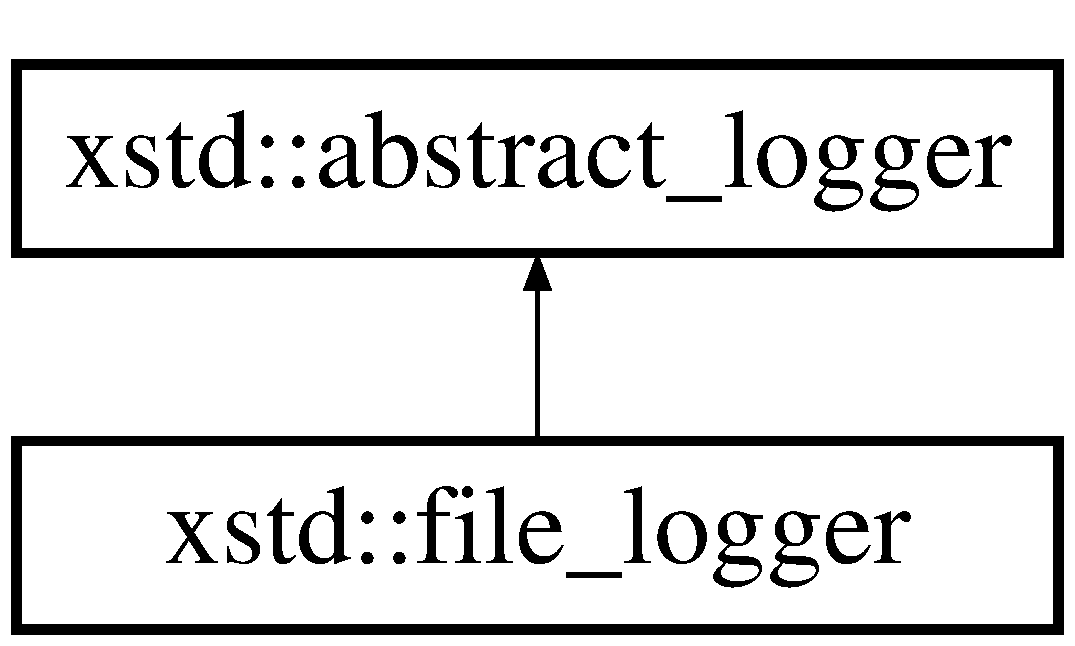
\includegraphics[height=2.000000cm]{classxstd_1_1file__logger}
\end{center}
\end{figure}
\subsection*{Public Member Functions}
\begin{DoxyCompactItemize}
\item 
\hyperlink{classxstd_1_1file__logger_a6e43dc8871b62e45550ce6470dcf5477}{file\-\_\-logger} (const std\-::string \&\hyperlink{classxstd_1_1file__logger_a0745eaab93df733f6696fa14e74eb068}{file}, bool \hyperlink{classxstd_1_1abstract__logger_a5216ec0a18fea2571db19d5a55d8700f}{add\-\_\-new\-\_\-line}=true, bool \hyperlink{classxstd_1_1abstract__logger_a534b4f6a3dcdd3b7f18abfcb1bb5b937}{add\-\_\-time\-\_\-stamp}=true) noexcept
\item 
void \hyperlink{classxstd_1_1abstract__logger_ad470970ac4726355f3423017f434ace8}{log} (const std\-::string \&data) const noexcept
\end{DoxyCompactItemize}
\subsection*{Public Attributes}
\begin{DoxyCompactItemize}
\item 
bool \hyperlink{classxstd_1_1abstract__logger_a5216ec0a18fea2571db19d5a55d8700f}{add\-\_\-new\-\_\-line}
\item 
bool \hyperlink{classxstd_1_1abstract__logger_a534b4f6a3dcdd3b7f18abfcb1bb5b937}{add\-\_\-time\-\_\-stamp}
\end{DoxyCompactItemize}
\subsection*{Protected Member Functions}
\begin{DoxyCompactItemize}
\item 
virtual void \hyperlink{classxstd_1_1file__logger_a806b0a7c20bad624afbddd2346312ca6}{log\-\_\-data} (const std\-::string \&data) const noexcept override
\item 
void \hyperlink{classxstd_1_1abstract__logger_a106b39652dd0d1efb32d8ad52ae6555c}{log\-\_\-new\-\_\-line} (void) const noexcept
\item 
void \hyperlink{classxstd_1_1abstract__logger_a8bed4dfa79399f58146700adfd1ac06f}{log\-\_\-time\-\_\-stamp} (void) const noexcept
\end{DoxyCompactItemize}
\subsection*{Static Protected Member Functions}
\begin{DoxyCompactItemize}
\item 
static std\-::string \hyperlink{classxstd_1_1abstract__logger_a1077a739173ed39b8f71f0ef69ada29f}{make\-\_\-time\-\_\-stamp} (void) noexcept
\end{DoxyCompactItemize}
\subsection*{Protected Attributes}
\begin{DoxyCompactItemize}
\item 
std\-::string \hyperlink{classxstd_1_1file__logger_a0745eaab93df733f6696fa14e74eb068}{file}
\end{DoxyCompactItemize}


\subsection{Constructor \& Destructor Documentation}
\hypertarget{classxstd_1_1file__logger_a6e43dc8871b62e45550ce6470dcf5477}{\index{xstd\-::file\-\_\-logger@{xstd\-::file\-\_\-logger}!file\-\_\-logger@{file\-\_\-logger}}
\index{file\-\_\-logger@{file\-\_\-logger}!xstd::file_logger@{xstd\-::file\-\_\-logger}}
\subsubsection[{file\-\_\-logger}]{\setlength{\rightskip}{0pt plus 5cm}xstd\-::file\-\_\-logger\-::file\-\_\-logger (
\begin{DoxyParamCaption}
\item[{const std\-::string \&}]{file, }
\item[{bool}]{add\-\_\-new\-\_\-line = {\ttfamily true}, }
\item[{bool}]{add\-\_\-time\-\_\-stamp = {\ttfamily true}}
\end{DoxyParamCaption}
)\hspace{0.3cm}{\ttfamily [inline]}, {\ttfamily [explicit]}}}\label{classxstd_1_1file__logger_a6e43dc8871b62e45550ce6470dcf5477}


\subsection{Member Function Documentation}
\hypertarget{classxstd_1_1abstract__logger_ad470970ac4726355f3423017f434ace8}{\index{xstd\-::file\-\_\-logger@{xstd\-::file\-\_\-logger}!log@{log}}
\index{log@{log}!xstd::file_logger@{xstd\-::file\-\_\-logger}}
\subsubsection[{log}]{\setlength{\rightskip}{0pt plus 5cm}void xstd\-::abstract\-\_\-logger\-::log (
\begin{DoxyParamCaption}
\item[{const std\-::string \&}]{data}
\end{DoxyParamCaption}
) const\hspace{0.3cm}{\ttfamily [inline]}, {\ttfamily [inherited]}}}\label{classxstd_1_1abstract__logger_ad470970ac4726355f3423017f434ace8}
\hypertarget{classxstd_1_1file__logger_a806b0a7c20bad624afbddd2346312ca6}{\index{xstd\-::file\-\_\-logger@{xstd\-::file\-\_\-logger}!log\-\_\-data@{log\-\_\-data}}
\index{log\-\_\-data@{log\-\_\-data}!xstd::file_logger@{xstd\-::file\-\_\-logger}}
\subsubsection[{log\-\_\-data}]{\setlength{\rightskip}{0pt plus 5cm}void xstd\-::file\-\_\-logger\-::log\-\_\-data (
\begin{DoxyParamCaption}
\item[{const std\-::string \&}]{data}
\end{DoxyParamCaption}
) const\hspace{0.3cm}{\ttfamily [inline]}, {\ttfamily [override]}, {\ttfamily [protected]}, {\ttfamily [virtual]}}}\label{classxstd_1_1file__logger_a806b0a7c20bad624afbddd2346312ca6}


Implements \hyperlink{classxstd_1_1abstract__logger_a8cf4f5fd1490b54680060022a2f8ac91}{xstd\-::abstract\-\_\-logger}.

\hypertarget{classxstd_1_1abstract__logger_a106b39652dd0d1efb32d8ad52ae6555c}{\index{xstd\-::file\-\_\-logger@{xstd\-::file\-\_\-logger}!log\-\_\-new\-\_\-line@{log\-\_\-new\-\_\-line}}
\index{log\-\_\-new\-\_\-line@{log\-\_\-new\-\_\-line}!xstd::file_logger@{xstd\-::file\-\_\-logger}}
\subsubsection[{log\-\_\-new\-\_\-line}]{\setlength{\rightskip}{0pt plus 5cm}void xstd\-::abstract\-\_\-logger\-::log\-\_\-new\-\_\-line (
\begin{DoxyParamCaption}
\item[{void}]{}
\end{DoxyParamCaption}
) const\hspace{0.3cm}{\ttfamily [inline]}, {\ttfamily [protected]}, {\ttfamily [inherited]}}}\label{classxstd_1_1abstract__logger_a106b39652dd0d1efb32d8ad52ae6555c}
\hypertarget{classxstd_1_1abstract__logger_a8bed4dfa79399f58146700adfd1ac06f}{\index{xstd\-::file\-\_\-logger@{xstd\-::file\-\_\-logger}!log\-\_\-time\-\_\-stamp@{log\-\_\-time\-\_\-stamp}}
\index{log\-\_\-time\-\_\-stamp@{log\-\_\-time\-\_\-stamp}!xstd::file_logger@{xstd\-::file\-\_\-logger}}
\subsubsection[{log\-\_\-time\-\_\-stamp}]{\setlength{\rightskip}{0pt plus 5cm}void xstd\-::abstract\-\_\-logger\-::log\-\_\-time\-\_\-stamp (
\begin{DoxyParamCaption}
\item[{void}]{}
\end{DoxyParamCaption}
) const\hspace{0.3cm}{\ttfamily [inline]}, {\ttfamily [protected]}, {\ttfamily [inherited]}}}\label{classxstd_1_1abstract__logger_a8bed4dfa79399f58146700adfd1ac06f}
\hypertarget{classxstd_1_1abstract__logger_a1077a739173ed39b8f71f0ef69ada29f}{\index{xstd\-::file\-\_\-logger@{xstd\-::file\-\_\-logger}!make\-\_\-time\-\_\-stamp@{make\-\_\-time\-\_\-stamp}}
\index{make\-\_\-time\-\_\-stamp@{make\-\_\-time\-\_\-stamp}!xstd::file_logger@{xstd\-::file\-\_\-logger}}
\subsubsection[{make\-\_\-time\-\_\-stamp}]{\setlength{\rightskip}{0pt plus 5cm}std\-::string xstd\-::abstract\-\_\-logger\-::make\-\_\-time\-\_\-stamp (
\begin{DoxyParamCaption}
\item[{void}]{}
\end{DoxyParamCaption}
)\hspace{0.3cm}{\ttfamily [inline]}, {\ttfamily [static]}, {\ttfamily [protected]}, {\ttfamily [inherited]}}}\label{classxstd_1_1abstract__logger_a1077a739173ed39b8f71f0ef69ada29f}


\subsection{Member Data Documentation}
\hypertarget{classxstd_1_1abstract__logger_a5216ec0a18fea2571db19d5a55d8700f}{\index{xstd\-::file\-\_\-logger@{xstd\-::file\-\_\-logger}!add\-\_\-new\-\_\-line@{add\-\_\-new\-\_\-line}}
\index{add\-\_\-new\-\_\-line@{add\-\_\-new\-\_\-line}!xstd::file_logger@{xstd\-::file\-\_\-logger}}
\subsubsection[{add\-\_\-new\-\_\-line}]{\setlength{\rightskip}{0pt plus 5cm}bool xstd\-::abstract\-\_\-logger\-::add\-\_\-new\-\_\-line\hspace{0.3cm}{\ttfamily [inherited]}}}\label{classxstd_1_1abstract__logger_a5216ec0a18fea2571db19d5a55d8700f}
\hypertarget{classxstd_1_1abstract__logger_a534b4f6a3dcdd3b7f18abfcb1bb5b937}{\index{xstd\-::file\-\_\-logger@{xstd\-::file\-\_\-logger}!add\-\_\-time\-\_\-stamp@{add\-\_\-time\-\_\-stamp}}
\index{add\-\_\-time\-\_\-stamp@{add\-\_\-time\-\_\-stamp}!xstd::file_logger@{xstd\-::file\-\_\-logger}}
\subsubsection[{add\-\_\-time\-\_\-stamp}]{\setlength{\rightskip}{0pt plus 5cm}bool xstd\-::abstract\-\_\-logger\-::add\-\_\-time\-\_\-stamp\hspace{0.3cm}{\ttfamily [inherited]}}}\label{classxstd_1_1abstract__logger_a534b4f6a3dcdd3b7f18abfcb1bb5b937}
\hypertarget{classxstd_1_1file__logger_a0745eaab93df733f6696fa14e74eb068}{\index{xstd\-::file\-\_\-logger@{xstd\-::file\-\_\-logger}!file@{file}}
\index{file@{file}!xstd::file_logger@{xstd\-::file\-\_\-logger}}
\subsubsection[{file}]{\setlength{\rightskip}{0pt plus 5cm}std\-::string xstd\-::file\-\_\-logger\-::file\hspace{0.3cm}{\ttfamily [protected]}}}\label{classxstd_1_1file__logger_a0745eaab93df733f6696fa14e74eb068}


The documentation for this class was generated from the following files\-:\begin{DoxyCompactItemize}
\item 
src/log/file\-\_\-logger/src/\hyperlink{file__logger_8hpp}{file\-\_\-logger.\-hpp}\item 
src/log/file\-\_\-logger/src/\hyperlink{file__logger_8ipp}{file\-\_\-logger.\-ipp}\end{DoxyCompactItemize}

\hypertarget{structxstd_1_1pp_1_1first__type}{\section{xstd\-:\-:pp\-:\-:first\-\_\-type$<$ parameters\-\_\-types $>$ Struct Template Reference}
\label{structxstd_1_1pp_1_1first__type}\index{xstd\-::pp\-::first\-\_\-type$<$ parameters\-\_\-types $>$@{xstd\-::pp\-::first\-\_\-type$<$ parameters\-\_\-types $>$}}
}


{\ttfamily \#include $<$parameter\-\_\-pack\-\_\-element\-\_\-type.\-hpp$>$}



The documentation for this struct was generated from the following file\-:\begin{DoxyCompactItemize}
\item 
src/utility/parameter\-\_\-pack/parameter\-\_\-pack\-\_\-element\-\_\-type/src/\hyperlink{parameter__pack__element__type_8hpp}{parameter\-\_\-pack\-\_\-element\-\_\-type.\-hpp}\end{DoxyCompactItemize}

\hypertarget{classxstd_1_1functor}{\section{xstd\-:\-:functor$<$ object\-\_\-type, arguments\-\_\-type $>$ Class Template Reference}
\label{classxstd_1_1functor}\index{xstd\-::functor$<$ object\-\_\-type, arguments\-\_\-type $>$@{xstd\-::functor$<$ object\-\_\-type, arguments\-\_\-type $>$}}
}
Inheritance diagram for xstd\-:\-:functor$<$ object\-\_\-type, arguments\-\_\-type $>$\-:\begin{figure}[H]
\begin{center}
\leavevmode
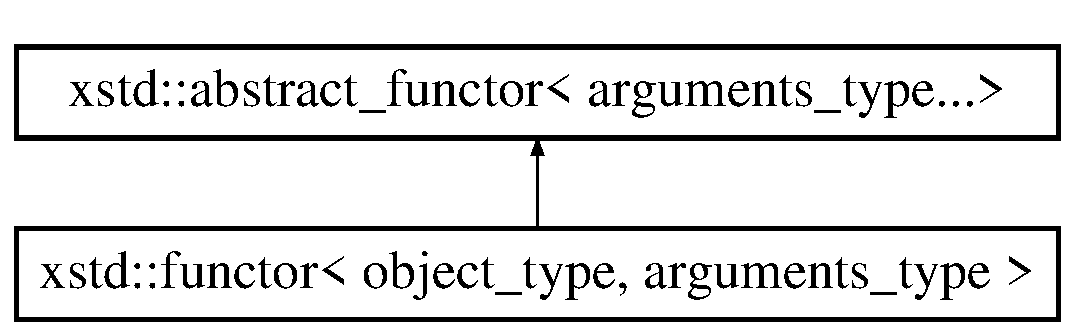
\includegraphics[height=2.000000cm]{classxstd_1_1functor}
\end{center}
\end{figure}
\subsection*{Public Member Functions}
\begin{DoxyCompactItemize}
\item 
\hypertarget{classxstd_1_1functor_aed2d510d4df5f6bb33d06370fbfa5fb8}{{\bfseries functor} (object\-\_\-type $\ast$object\-\_\-ptr, void(object\-\_\-type\-::$\ast$method\-\_\-ptr)(arguments\-\_\-type...))}\label{classxstd_1_1functor_aed2d510d4df5f6bb33d06370fbfa5fb8}

\item 
\hypertarget{classxstd_1_1functor_aeb8b8bd83b493e203d526dbf6b0c4920}{virtual void {\bfseries operator()} (arguments\-\_\-type...\-arguments) const override final}\label{classxstd_1_1functor_aeb8b8bd83b493e203d526dbf6b0c4920}

\item 
\hypertarget{classxstd_1_1functor_aa40709e615299c2c2d05c8c21c7ace66}{virtual void {\bfseries invoke} (arguments\-\_\-type...\-arguments) const override final}\label{classxstd_1_1functor_aa40709e615299c2c2d05c8c21c7ace66}

\end{DoxyCompactItemize}
\subsection*{Public Attributes}
\begin{DoxyCompactItemize}
\item 
\hypertarget{classxstd_1_1functor_a673d0ccf7da14d0d7f4726bbdf8af8a4}{void(object\-\_\-type\-::$\ast$ {\bfseries method\-\_\-ptr} )(arguments\-\_\-type...)}\label{classxstd_1_1functor_a673d0ccf7da14d0d7f4726bbdf8af8a4}

\item 
\hypertarget{classxstd_1_1functor_a919d42ea50702cf2ff02360f175b02ad}{object\-\_\-type $\ast$ {\bfseries object\-\_\-ptr}}\label{classxstd_1_1functor_a919d42ea50702cf2ff02360f175b02ad}

\end{DoxyCompactItemize}


The documentation for this class was generated from the following file\-:\begin{DoxyCompactItemize}
\item 
src/functional/functor/functor/src/functor.\-hpp\end{DoxyCompactItemize}

\hypertarget{structxstd_1_1pp_1_1is__heterogeneous}{\section{xstd\-:\-:pp\-:\-:is\-\_\-heterogeneous$<$ parameters\-\_\-types $>$ Struct Template Reference}
\label{structxstd_1_1pp_1_1is__heterogeneous}\index{xstd\-::pp\-::is\-\_\-heterogeneous$<$ parameters\-\_\-types $>$@{xstd\-::pp\-::is\-\_\-heterogeneous$<$ parameters\-\_\-types $>$}}
}


{\ttfamily \#include $<$parameter\-\_\-pack\-\_\-homogeneity.\-hpp$>$}

\subsection*{Static Public Attributes}
\begin{DoxyCompactItemize}
\item 
static const bool \hyperlink{structxstd_1_1pp_1_1is__heterogeneous_a790c8cb5a84cf3da91bf1602e181105b}{value} = ! \hyperlink{structxstd_1_1pp_1_1is__homogeneous}{is\-\_\-homogeneous}$<$parameters\-\_\-types...$>$\-::value
\end{DoxyCompactItemize}


\subsection{Member Data Documentation}
\hypertarget{structxstd_1_1pp_1_1is__heterogeneous_a790c8cb5a84cf3da91bf1602e181105b}{\index{xstd\-::pp\-::is\-\_\-heterogeneous@{xstd\-::pp\-::is\-\_\-heterogeneous}!value@{value}}
\index{value@{value}!xstd::pp::is_heterogeneous@{xstd\-::pp\-::is\-\_\-heterogeneous}}
\subsubsection[{value}]{\setlength{\rightskip}{0pt plus 5cm}template$<$typename... parameters\-\_\-types$>$ const bool {\bf xstd\-::pp\-::is\-\_\-heterogeneous}$<$ parameters\-\_\-types $>$\-::value = ! {\bf is\-\_\-homogeneous}$<$parameters\-\_\-types...$>$\-::value\hspace{0.3cm}{\ttfamily [static]}}}\label{structxstd_1_1pp_1_1is__heterogeneous_a790c8cb5a84cf3da91bf1602e181105b}


The documentation for this struct was generated from the following file\-:\begin{DoxyCompactItemize}
\item 
src/utility/parameter\-\_\-pack/parameter\-\_\-pack\-\_\-homogeneity/src/\hyperlink{parameter__pack__homogeneity_8hpp}{parameter\-\_\-pack\-\_\-homogeneity.\-hpp}\end{DoxyCompactItemize}

\hypertarget{structxstd_1_1pp_1_1is__homogeneous}{\section{xstd\-:\-:pp\-:\-:is\-\_\-homogeneous$<$ parameters\-\_\-types $>$ Struct Template Reference}
\label{structxstd_1_1pp_1_1is__homogeneous}\index{xstd\-::pp\-::is\-\_\-homogeneous$<$ parameters\-\_\-types $>$@{xstd\-::pp\-::is\-\_\-homogeneous$<$ parameters\-\_\-types $>$}}
}
\subsection*{Static Public Attributes}
\begin{DoxyCompactItemize}
\item 
\hypertarget{structxstd_1_1pp_1_1is__homogeneous_a104d1888e8f39e2d57ab27c7c3fb7383}{static const bool {\bfseries value} = true}\label{structxstd_1_1pp_1_1is__homogeneous_a104d1888e8f39e2d57ab27c7c3fb7383}

\end{DoxyCompactItemize}


The documentation for this struct was generated from the following file\-:\begin{DoxyCompactItemize}
\item 
src/utility/parameter\-\_\-pack/parameter\-\_\-pack\-\_\-homogeneity/src/parameter\-\_\-pack\-\_\-homogeneity.\-hpp\end{DoxyCompactItemize}

\hypertarget{structxstd_1_1pp_1_1is__homogeneous_3_01first__parameter__type_00_01other__parameters__types_8_8_8_01_4}{\section{xstd\-:\-:pp\-:\-:is\-\_\-homogeneous$<$ first\-\_\-parameter\-\_\-type, other\-\_\-parameters\-\_\-types... $>$ Struct Template Reference}
\label{structxstd_1_1pp_1_1is__homogeneous_3_01first__parameter__type_00_01other__parameters__types_8_8_8_01_4}\index{xstd\-::pp\-::is\-\_\-homogeneous$<$ first\-\_\-parameter\-\_\-type, other\-\_\-parameters\-\_\-types... $>$@{xstd\-::pp\-::is\-\_\-homogeneous$<$ first\-\_\-parameter\-\_\-type, other\-\_\-parameters\-\_\-types... $>$}}
}
\subsection*{Static Public Attributes}
\begin{DoxyCompactItemize}
\item 
\hypertarget{structxstd_1_1pp_1_1is__homogeneous_3_01first__parameter__type_00_01other__parameters__types_8_8_8_01_4_a7cb56d449b90e1ffbc9e9332d1faaa94}{static const bool {\bfseries value} = std\-::is\-\_\-same$<$first\-\_\-parameter\-\_\-type,other\-\_\-parameters\-\_\-type$>$\-::value}\label{structxstd_1_1pp_1_1is__homogeneous_3_01first__parameter__type_00_01other__parameters__types_8_8_8_01_4_a7cb56d449b90e1ffbc9e9332d1faaa94}

\end{DoxyCompactItemize}


The documentation for this struct was generated from the following file\-:\begin{DoxyCompactItemize}
\item 
src/utility/parameter\-\_\-pack/parameter\-\_\-pack\-\_\-homogeneity/src/parameter\-\_\-pack\-\_\-homogeneity.\-hpp\end{DoxyCompactItemize}

\hypertarget{structxstd_1_1pp_1_1is__homogeneous_3_01parameter__type_01_4}{\section{xstd\-:\-:pp\-:\-:is\-\_\-homogeneous$<$ parameter\-\_\-type $>$ Struct Template Reference}
\label{structxstd_1_1pp_1_1is__homogeneous_3_01parameter__type_01_4}\index{xstd\-::pp\-::is\-\_\-homogeneous$<$ parameter\-\_\-type $>$@{xstd\-::pp\-::is\-\_\-homogeneous$<$ parameter\-\_\-type $>$}}
}


{\ttfamily \#include $<$parameter\-\_\-pack\-\_\-homogeneity.\-hpp$>$}

\subsection*{Static Public Attributes}
\begin{DoxyCompactItemize}
\item 
static const bool \hyperlink{structxstd_1_1pp_1_1is__homogeneous_3_01parameter__type_01_4_a827e8f99e9ec9a203c3851ecd58dddb6}{value} = true
\end{DoxyCompactItemize}


\subsection{Member Data Documentation}
\hypertarget{structxstd_1_1pp_1_1is__homogeneous_3_01parameter__type_01_4_a827e8f99e9ec9a203c3851ecd58dddb6}{\index{xstd\-::pp\-::is\-\_\-homogeneous$<$ parameter\-\_\-type $>$@{xstd\-::pp\-::is\-\_\-homogeneous$<$ parameter\-\_\-type $>$}!value@{value}}
\index{value@{value}!xstd::pp::is_homogeneous< parameter_type >@{xstd\-::pp\-::is\-\_\-homogeneous$<$ parameter\-\_\-type $>$}}
\subsubsection[{value}]{\setlength{\rightskip}{0pt plus 5cm}template$<$typename parameter\-\_\-type $>$ const bool {\bf xstd\-::pp\-::is\-\_\-homogeneous}$<$ parameter\-\_\-type $>$\-::value = true\hspace{0.3cm}{\ttfamily [static]}}}\label{structxstd_1_1pp_1_1is__homogeneous_3_01parameter__type_01_4_a827e8f99e9ec9a203c3851ecd58dddb6}


The documentation for this struct was generated from the following file\-:\begin{DoxyCompactItemize}
\item 
src/utility/parameter\-\_\-pack/parameter\-\_\-pack\-\_\-homogeneity/src/\hyperlink{parameter__pack__homogeneity_8hpp}{parameter\-\_\-pack\-\_\-homogeneity.\-hpp}\end{DoxyCompactItemize}

\hypertarget{structxstd_1_1pp_1_1last__type}{\section{xstd\-:\-:pp\-:\-:last\-\_\-type$<$ parameters\-\_\-types $>$ Struct Template Reference}
\label{structxstd_1_1pp_1_1last__type}\index{xstd\-::pp\-::last\-\_\-type$<$ parameters\-\_\-types $>$@{xstd\-::pp\-::last\-\_\-type$<$ parameters\-\_\-types $>$}}
}


{\ttfamily \#include $<$parameter\-\_\-pack\-\_\-element\-\_\-type.\-hpp$>$}



The documentation for this struct was generated from the following file\-:\begin{DoxyCompactItemize}
\item 
src/utility/parameter\-\_\-pack/parameter\-\_\-pack\-\_\-element\-\_\-type/src/\hyperlink{parameter__pack__element__type_8hpp}{parameter\-\_\-pack\-\_\-element\-\_\-type.\-hpp}\end{DoxyCompactItemize}

\hypertarget{classxstd_1_1logger__client}{\section{xstd\-:\-:logger\-\_\-client Class Reference}
\label{classxstd_1_1logger__client}\index{xstd\-::logger\-\_\-client@{xstd\-::logger\-\_\-client}}
}
\subsection*{Public Member Functions}
\begin{DoxyCompactItemize}
\item 
\hypertarget{classxstd_1_1logger__client_ae366adb742d038fa072522500d798ce8}{{\bfseries logger\-\_\-client} (\hyperlink{classxstd_1_1abstract__logger}{abstract\-\_\-logger} $\ast$logger\-\_\-ptr=nullptr)}\label{classxstd_1_1logger__client_ae366adb742d038fa072522500d798ce8}

\item 
\hypertarget{classxstd_1_1logger__client_a4567aa30484c31b0d53089d1d08f8fab}{\hyperlink{classxstd_1_1abstract__logger}{abstract\-\_\-logger} \& {\bfseries get\-\_\-logger\-\_\-ref} (void)}\label{classxstd_1_1logger__client_a4567aa30484c31b0d53089d1d08f8fab}

\item 
\hypertarget{classxstd_1_1logger__client_a436c05e8f5d01fa5ed01aea36d1c5390}{\hyperlink{classxstd_1_1abstract__logger}{abstract\-\_\-logger} $\ast$ {\bfseries get\-\_\-logger\-\_\-ptr} (void)}\label{classxstd_1_1logger__client_a436c05e8f5d01fa5ed01aea36d1c5390}

\item 
\hypertarget{classxstd_1_1logger__client_a058f72e775905783e79721ecb2a65349}{void {\bfseries set\-\_\-logger} (\hyperlink{classxstd_1_1abstract__logger}{abstract\-\_\-logger} $\ast$logger\-\_\-ptr=nullptr)}\label{classxstd_1_1logger__client_a058f72e775905783e79721ecb2a65349}

\item 
\hypertarget{classxstd_1_1logger__client_a7169793d2c5512150d611ae47e0c6b74}{void {\bfseries log} (const std\-::string \&data) const }\label{classxstd_1_1logger__client_a7169793d2c5512150d611ae47e0c6b74}

\end{DoxyCompactItemize}
\subsection*{Protected Attributes}
\begin{DoxyCompactItemize}
\item 
\hypertarget{classxstd_1_1logger__client_a6f1cc6e74cfa370ec516e3fa792b3f1c}{\hyperlink{classxstd_1_1abstract__logger}{abstract\-\_\-logger} $\ast$ {\bfseries logger\-\_\-ptr}}\label{classxstd_1_1logger__client_a6f1cc6e74cfa370ec516e3fa792b3f1c}

\end{DoxyCompactItemize}


The documentation for this class was generated from the following files\-:\begin{DoxyCompactItemize}
\item 
src/log/logger\-\_\-client/src/logger\-\_\-client.\-hpp\item 
src/log/logger\-\_\-client/src/logger\-\_\-client.\-ipp\end{DoxyCompactItemize}

\hypertarget{structxstd_1_1pp_1_1nth__type}{\section{xstd\-:\-:pp\-:\-:nth\-\_\-type$<$ parameter\-\_\-id, parameters\-\_\-types $>$ Struct Template Reference}
\label{structxstd_1_1pp_1_1nth__type}\index{xstd\-::pp\-::nth\-\_\-type$<$ parameter\-\_\-id, parameters\-\_\-types $>$@{xstd\-::pp\-::nth\-\_\-type$<$ parameter\-\_\-id, parameters\-\_\-types $>$}}
}


{\ttfamily \#include $<$parameter\-\_\-pack\-\_\-element\-\_\-type.\-hpp$>$}



The documentation for this struct was generated from the following file\-:\begin{DoxyCompactItemize}
\item 
src/utility/parameter\-\_\-pack/parameter\-\_\-pack\-\_\-element\-\_\-type/src/\hyperlink{parameter__pack__element__type_8hpp}{parameter\-\_\-pack\-\_\-element\-\_\-type.\-hpp}\end{DoxyCompactItemize}

\hypertarget{structxstd_1_1pp_1_1nth__type__helper}{\section{xstd\-:\-:pp\-:\-:nth\-\_\-type\-\_\-helper$<$ parameter\-\_\-id, parameters\-\_\-types $>$ Struct Template Reference}
\label{structxstd_1_1pp_1_1nth__type__helper}\index{xstd\-::pp\-::nth\-\_\-type\-\_\-helper$<$ parameter\-\_\-id, parameters\-\_\-types $>$@{xstd\-::pp\-::nth\-\_\-type\-\_\-helper$<$ parameter\-\_\-id, parameters\-\_\-types $>$}}
}


{\ttfamily \#include $<$parameter\-\_\-pack\-\_\-element\-\_\-type.\-hpp$>$}



The documentation for this struct was generated from the following file\-:\begin{DoxyCompactItemize}
\item 
src/utility/parameter\-\_\-pack/parameter\-\_\-pack\-\_\-element\-\_\-type/src/\hyperlink{parameter__pack__element__type_8hpp}{parameter\-\_\-pack\-\_\-element\-\_\-type.\-hpp}\end{DoxyCompactItemize}

\hypertarget{structxstd_1_1pp_1_1nth__type__helper_3_010_00_01first__parameter__type_00_01other__parameters__types_8_8_8_01_4}{\section{xstd\-:\-:pp\-:\-:nth\-\_\-type\-\_\-helper$<$ 0, first\-\_\-parameter\-\_\-type, other\-\_\-parameters\-\_\-types... $>$ Struct Template Reference}
\label{structxstd_1_1pp_1_1nth__type__helper_3_010_00_01first__parameter__type_00_01other__parameters__types_8_8_8_01_4}\index{xstd\-::pp\-::nth\-\_\-type\-\_\-helper$<$ 0, first\-\_\-parameter\-\_\-type, other\-\_\-parameters\-\_\-types... $>$@{xstd\-::pp\-::nth\-\_\-type\-\_\-helper$<$ 0, first\-\_\-parameter\-\_\-type, other\-\_\-parameters\-\_\-types... $>$}}
}


The documentation for this struct was generated from the following file\-:\begin{DoxyCompactItemize}
\item 
src/utility/parameter\-\_\-pack/parameter\-\_\-pack\-\_\-element\-\_\-type/src/parameter\-\_\-pack\-\_\-element\-\_\-type.\-hpp\end{DoxyCompactItemize}

\hypertarget{structxstd_1_1pp_1_1nth__type__helper_3_01parameter__id_00_01first__parameter__type_00_01other__parameters__types_8_8_8_01_4}{\section{xstd\-:\-:pp\-:\-:nth\-\_\-type\-\_\-helper$<$ parameter\-\_\-id, first\-\_\-parameter\-\_\-type, other\-\_\-parameters\-\_\-types... $>$ Struct Template Reference}
\label{structxstd_1_1pp_1_1nth__type__helper_3_01parameter__id_00_01first__parameter__type_00_01other__parameters__types_8_8_8_01_4}\index{xstd\-::pp\-::nth\-\_\-type\-\_\-helper$<$ parameter\-\_\-id, first\-\_\-parameter\-\_\-type, other\-\_\-parameters\-\_\-types... $>$@{xstd\-::pp\-::nth\-\_\-type\-\_\-helper$<$ parameter\-\_\-id, first\-\_\-parameter\-\_\-type, other\-\_\-parameters\-\_\-types... $>$}}
}


The documentation for this struct was generated from the following file\-:\begin{DoxyCompactItemize}
\item 
src/utility/parameter\-\_\-pack/parameter\-\_\-pack\-\_\-element\-\_\-type/src/parameter\-\_\-pack\-\_\-element\-\_\-type.\-hpp\end{DoxyCompactItemize}

\hypertarget{structxstd_1_1pp_1_1null__type}{\section{xstd\-:\-:pp\-:\-:null\-\_\-type Struct Reference}
\label{structxstd_1_1pp_1_1null__type}\index{xstd\-::pp\-::null\-\_\-type@{xstd\-::pp\-::null\-\_\-type}}
}


{\ttfamily \#include $<$parameter\-\_\-pack\-\_\-element\-\_\-type.\-hpp$>$}

\subsection*{Public Member Functions}
\begin{DoxyCompactItemize}
\item 
bool \hyperlink{structxstd_1_1pp_1_1null__type_ab9e5487aa630bf4bfd0b01c28cc0415e}{operator==} (const \hyperlink{structxstd_1_1pp_1_1null__type}{null\-\_\-type}) const 
\item 
bool \hyperlink{structxstd_1_1pp_1_1null__type_ab290a23fbfc450daa1db57bfea446268}{operator!=} (const \hyperlink{structxstd_1_1pp_1_1null__type}{null\-\_\-type}) const 
\end{DoxyCompactItemize}


\subsection{Member Function Documentation}
\hypertarget{structxstd_1_1pp_1_1null__type_ab290a23fbfc450daa1db57bfea446268}{\index{xstd\-::pp\-::null\-\_\-type@{xstd\-::pp\-::null\-\_\-type}!operator!=@{operator!=}}
\index{operator!=@{operator!=}!xstd::pp::null_type@{xstd\-::pp\-::null\-\_\-type}}
\subsubsection[{operator!=}]{\setlength{\rightskip}{0pt plus 5cm}bool xstd\-::pp\-::null\-\_\-type\-::operator!= (
\begin{DoxyParamCaption}
\item[{const {\bf null\-\_\-type}}]{}
\end{DoxyParamCaption}
) const\hspace{0.3cm}{\ttfamily [inline]}}}\label{structxstd_1_1pp_1_1null__type_ab290a23fbfc450daa1db57bfea446268}
\hypertarget{structxstd_1_1pp_1_1null__type_ab9e5487aa630bf4bfd0b01c28cc0415e}{\index{xstd\-::pp\-::null\-\_\-type@{xstd\-::pp\-::null\-\_\-type}!operator==@{operator==}}
\index{operator==@{operator==}!xstd::pp::null_type@{xstd\-::pp\-::null\-\_\-type}}
\subsubsection[{operator==}]{\setlength{\rightskip}{0pt plus 5cm}bool xstd\-::pp\-::null\-\_\-type\-::operator== (
\begin{DoxyParamCaption}
\item[{const {\bf null\-\_\-type}}]{}
\end{DoxyParamCaption}
) const\hspace{0.3cm}{\ttfamily [inline]}}}\label{structxstd_1_1pp_1_1null__type_ab9e5487aa630bf4bfd0b01c28cc0415e}


The documentation for this struct was generated from the following file\-:\begin{DoxyCompactItemize}
\item 
src/utility/parameter\-\_\-pack/parameter\-\_\-pack\-\_\-element\-\_\-type/src/\hyperlink{parameter__pack__element__type_8hpp}{parameter\-\_\-pack\-\_\-element\-\_\-type.\-hpp}\end{DoxyCompactItemize}

\hypertarget{classxstd_1_1point}{\section{xstd\-:\-:point$<$ type, dimension $>$ Class Template Reference}
\label{classxstd_1_1point}\index{xstd\-::point$<$ type, dimension $>$@{xstd\-::point$<$ type, dimension $>$}}
}
\subsection*{Public Member Functions}
\begin{DoxyCompactItemize}
\item 
\hypertarget{classxstd_1_1point_a31b7e462164c6071b3847b0ad0604ef0}{{\bfseries point} (const coordinates\-\_\-initializer\-\_\-list \&coordinates\-\_\-object)}\label{classxstd_1_1point_a31b7e462164c6071b3847b0ad0604ef0}

\item 
\hypertarget{classxstd_1_1point_a3895117f5b9d43c53a8da93528aba6f5}{{\footnotesize template$<$typename \-\_\-type $>$ }\\{\bfseries point} (const \hyperlink{classxstd_1_1point}{point}$<$ \-\_\-type, dimension $>$ \&point\-\_\-object)}\label{classxstd_1_1point_a3895117f5b9d43c53a8da93528aba6f5}

\item 
\hypertarget{classxstd_1_1point_a67d8aba62c4ebe7cf114a276e30336f2}{{\footnotesize template$<$typename \-\_\-type $>$ }\\\hyperlink{classxstd_1_1point}{point} \& {\bfseries operator=} (const \hyperlink{classxstd_1_1point}{point}$<$ \-\_\-type, dimension $>$ \&point\-\_\-object)}\label{classxstd_1_1point_a67d8aba62c4ebe7cf114a276e30336f2}

\item 
\hypertarget{classxstd_1_1point_aaf46d8e0e0676b0fb5e8d86a7742e2a1}{type \& {\bfseries operator\mbox{[}$\,$\mbox{]}} (const int coordinate\-Id)}\label{classxstd_1_1point_aaf46d8e0e0676b0fb5e8d86a7742e2a1}

\item 
\hypertarget{classxstd_1_1point_a39217029d54ae1c115cc79db3edc1e48}{const type \& {\bfseries operator\mbox{[}$\,$\mbox{]}} (const int coordinate\-Id) const }\label{classxstd_1_1point_a39217029d54ae1c115cc79db3edc1e48}

\item 
\hypertarget{classxstd_1_1point_a2f98209745efac5775e14315b58d5a1d}{{\footnotesize template$<$typename \-\_\-type $>$ }\\bool {\bfseries operator==} (const \hyperlink{classxstd_1_1point}{point}$<$ \-\_\-type, dimension $>$ \&point\-\_\-object) const }\label{classxstd_1_1point_a2f98209745efac5775e14315b58d5a1d}

\item 
\hypertarget{classxstd_1_1point_a41ffcfd2fbb0420aceb7a3d81950e945}{{\footnotesize template$<$typename \-\_\-type $>$ }\\bool {\bfseries operator!=} (const \hyperlink{classxstd_1_1point}{point}$<$ \-\_\-type, dimension $>$ \&point\-\_\-object) const }\label{classxstd_1_1point_a41ffcfd2fbb0420aceb7a3d81950e945}

\item 
\hypertarget{classxstd_1_1point_aae13ce0401101be7b26121f8be146f4b}{{\footnotesize template$<$typename \-\_\-type $>$ }\\\hyperlink{classxstd_1_1point}{point} {\bfseries operator+} (const \hyperlink{classxstd_1_1point}{point}$<$ \-\_\-type, dimension $>$ \&point\-\_\-object) const }\label{classxstd_1_1point_aae13ce0401101be7b26121f8be146f4b}

\item 
\hypertarget{classxstd_1_1point_ad1af00d4517e769e7da57cd26732a6ab}{{\footnotesize template$<$typename \-\_\-type $>$ }\\\hyperlink{classxstd_1_1point}{point} {\bfseries operator-\/} (const \hyperlink{classxstd_1_1point}{point}$<$ \-\_\-type, dimension $>$ \&point\-\_\-object) const }\label{classxstd_1_1point_ad1af00d4517e769e7da57cd26732a6ab}

\item 
\hypertarget{classxstd_1_1point_ac777d5594b34c30fe27bcd549ef89be4}{\hyperlink{classxstd_1_1point}{point} {\bfseries operator$\ast$} (const float multiplier) const }\label{classxstd_1_1point_ac777d5594b34c30fe27bcd549ef89be4}

\item 
\hypertarget{classxstd_1_1point_aa96d22aaf0a1687325dadaa832740c3e}{\hyperlink{classxstd_1_1point}{point} {\bfseries operator/} (const float multiplier) const }\label{classxstd_1_1point_aa96d22aaf0a1687325dadaa832740c3e}

\item 
\hypertarget{classxstd_1_1point_a766d0887be589b7448696e0c0b00d557}{int {\bfseries get\-\_\-dimension} (void) const }\label{classxstd_1_1point_a766d0887be589b7448696e0c0b00d557}

\item 
\hypertarget{classxstd_1_1point_ae0363f79e01bb646555c51dfd99444ca}{type {\bfseries get\-\_\-coordinate\-\_\-value} (const int coordinate\-Id) const }\label{classxstd_1_1point_ae0363f79e01bb646555c51dfd99444ca}

\item 
\hypertarget{classxstd_1_1point_a812c6e9c6b5e329897fbab3ccce407e7}{coordinates \& {\bfseries get\-\_\-coordinates\-\_\-ref} (void)}\label{classxstd_1_1point_a812c6e9c6b5e329897fbab3ccce407e7}

\item 
\hypertarget{classxstd_1_1point_aa6910f3a870a3844003ed1fa77dab3b9}{const coordinates \& {\bfseries get\-\_\-coordinates\-\_\-ref} (void) const }\label{classxstd_1_1point_aa6910f3a870a3844003ed1fa77dab3b9}

\item 
\hypertarget{classxstd_1_1point_a1926a1a02d788b584e7e994edb956d61}{{\footnotesize template$<$typename \-\_\-type $>$ }\\float {\bfseries get\-\_\-distance\-\_\-to} (const \hyperlink{classxstd_1_1point}{point}$<$ \-\_\-type, dimension $>$ \&point\-\_\-object) const }\label{classxstd_1_1point_a1926a1a02d788b584e7e994edb956d61}

\item 
\hypertarget{classxstd_1_1point_a468d82213633b70cb8c01f97838e6d49}{{\footnotesize template$<$typename \-\_\-type $>$ }\\void {\bfseries set\-\_\-coordinates\-\_\-values} (const \-\_\-type \&coordinates\-Value)}\label{classxstd_1_1point_a468d82213633b70cb8c01f97838e6d49}

\item 
\hypertarget{classxstd_1_1point_a239dbdfe4d96a38b9eacd76e972897c4}{void {\bfseries set\-\_\-coordinates\-\_\-values} (const coordinates\-\_\-initializer\-\_\-list \&coordinates\-\_\-object)}\label{classxstd_1_1point_a239dbdfe4d96a38b9eacd76e972897c4}

\item 
\hypertarget{classxstd_1_1point_a16ea81630c6918bca7393e7ce46e1691}{{\footnotesize template$<$typename \-\_\-type $>$ }\\void {\bfseries set\-\_\-coordinates\-\_\-values} (const std\-::array$<$ \-\_\-type, dimension $>$ \&coordinates\-\_\-object)}\label{classxstd_1_1point_a16ea81630c6918bca7393e7ce46e1691}

\item 
\hypertarget{classxstd_1_1point_a5e32aa4388cfc0d9b9b3df56c5d8bd91}{void {\bfseries validate\-\_\-dimension\-\_\-match} (const coordinates\-\_\-initializer\-\_\-list \&coordinates\-\_\-object) const }\label{classxstd_1_1point_a5e32aa4388cfc0d9b9b3df56c5d8bd91}

\item 
\hypertarget{classxstd_1_1point_a15edf9d511dcd8d27c98e77b18033573}{{\footnotesize template$<$typename \-\_\-type , int \-\_\-dimension$>$ }\\void {\bfseries validate\-\_\-dimension\-\_\-match} (const \hyperlink{classxstd_1_1point}{point}$<$ \-\_\-type, \-\_\-dimension $>$ \&) const }\label{classxstd_1_1point_a15edf9d511dcd8d27c98e77b18033573}

\item 
\hypertarget{classxstd_1_1point_a9c83662efe0927f03cb9cb1cfab796cd}{void {\bfseries validate\-\_\-coordinate\-\_\-id} (const int coordinate\-Id) const }\label{classxstd_1_1point_a9c83662efe0927f03cb9cb1cfab796cd}

\item 
\hypertarget{classxstd_1_1point_a1d9e30c142c79d1c21bdb271c81dabb5}{void {\bfseries validate\-\_\-dimension} (void) const }\label{classxstd_1_1point_a1d9e30c142c79d1c21bdb271c81dabb5}

\end{DoxyCompactItemize}
\subsection*{Protected Attributes}
\begin{DoxyCompactItemize}
\item 
\hypertarget{classxstd_1_1point_a6ee0acdc7f3fdd004426279d0d7963e6}{coordinates {\bfseries coordinates\-\_\-object}}\label{classxstd_1_1point_a6ee0acdc7f3fdd004426279d0d7963e6}

\end{DoxyCompactItemize}
\subsection*{Friends}
\begin{DoxyCompactItemize}
\item 
\hypertarget{classxstd_1_1point_a26f9c85c349535d8d87c0b2b4dda134e}{std\-::ostream \& {\bfseries operator$<$$<$} (std\-::ostream \&output\-Stream, const \hyperlink{classxstd_1_1point}{point} \&point\-\_\-object)}\label{classxstd_1_1point_a26f9c85c349535d8d87c0b2b4dda134e}

\end{DoxyCompactItemize}


The documentation for this class was generated from the following file\-:\begin{DoxyCompactItemize}
\item 
src/cmath/point/src/point.\-hpp\end{DoxyCompactItemize}

\hypertarget{structprinter}{\section{printer Struct Reference}
\label{structprinter}\index{printer@{printer}}
}
\subsection*{Static Public Member Functions}
\begin{DoxyCompactItemize}
\item 
\hypertarget{structprinter_a65d06f6b703eabfd57600550b27ef2ff}{{\footnotesize template$<$typename type $>$ }\\static void {\bfseries process} (type object)}\label{structprinter_a65d06f6b703eabfd57600550b27ef2ff}

\end{DoxyCompactItemize}


The documentation for this struct was generated from the following file\-:\begin{DoxyCompactItemize}
\item 
src/utility/parameter\-\_\-pack/parameter\-\_\-pack\-\_\-for\-\_\-each/tests/src/parameter\-\_\-pack\-\_\-for\-\_\-each\-\_\-tests.\-cpp\end{DoxyCompactItemize}

\hypertarget{classxstd_1_1raii__thread}{\section{xstd\-:\-:raii\-\_\-thread Class Reference}
\label{classxstd_1_1raii__thread}\index{xstd\-::raii\-\_\-thread@{xstd\-::raii\-\_\-thread}}
}
Inheritance diagram for xstd\-:\-:raii\-\_\-thread\-:\begin{figure}[H]
\begin{center}
\leavevmode
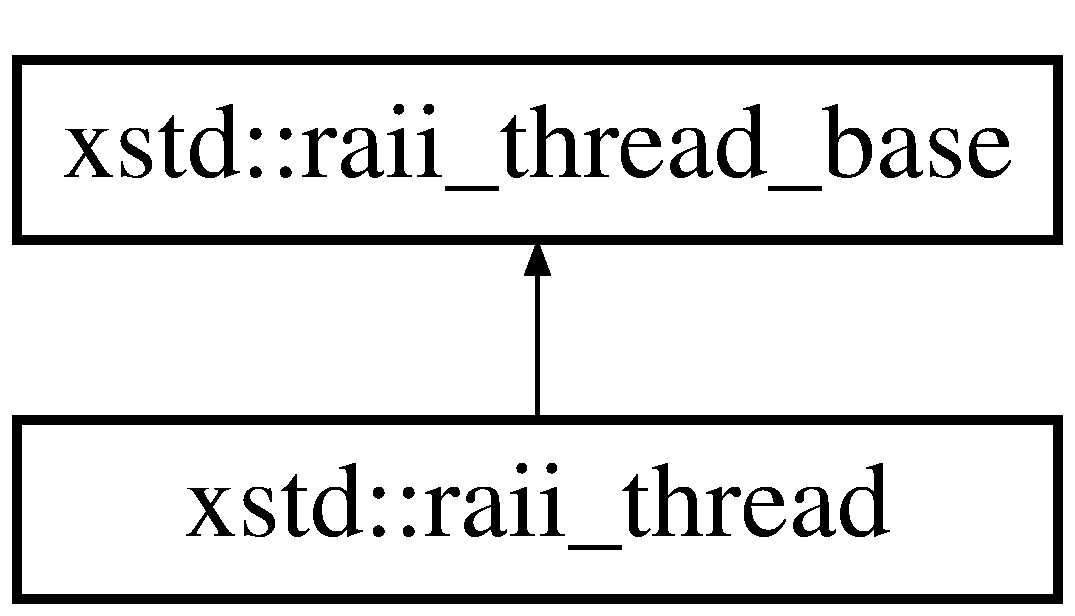
\includegraphics[height=2.000000cm]{classxstd_1_1raii__thread}
\end{center}
\end{figure}
\subsection*{Public Member Functions}
\begin{DoxyCompactItemize}
\item 
\hypertarget{classxstd_1_1raii__thread_a8bc39a85a55f9becb860febe87f9175c}{{\bfseries raii\-\_\-thread} (std\-::function$<$ void()$>$ client\-\_\-routine)}\label{classxstd_1_1raii__thread_a8bc39a85a55f9becb860febe87f9175c}

\end{DoxyCompactItemize}
\subsection*{Additional Inherited Members}


The documentation for this class was generated from the following files\-:\begin{DoxyCompactItemize}
\item 
src/thread/raii\-\_\-thread/src/raii\-\_\-thread.\-hpp\item 
src/thread/raii\-\_\-thread/src/raii\-\_\-thread.\-ipp\end{DoxyCompactItemize}

\hypertarget{classxstd_1_1raii__thread__base}{\section{xstd\-:\-:raii\-\_\-thread\-\_\-base Class Reference}
\label{classxstd_1_1raii__thread__base}\index{xstd\-::raii\-\_\-thread\-\_\-base@{xstd\-::raii\-\_\-thread\-\_\-base}}
}
Inheritance diagram for xstd\-:\-:raii\-\_\-thread\-\_\-base\-:\begin{figure}[H]
\begin{center}
\leavevmode
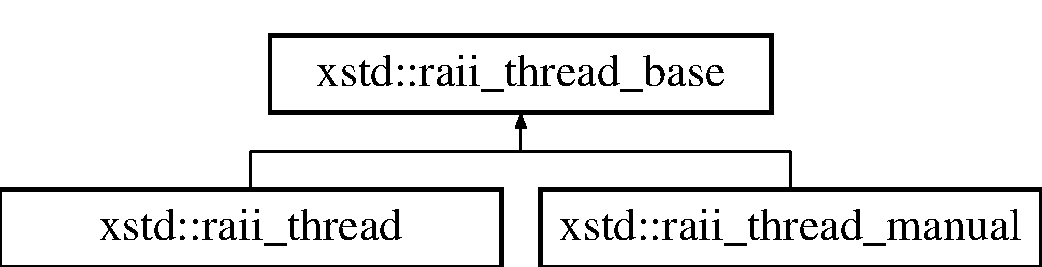
\includegraphics[height=2.000000cm]{classxstd_1_1raii__thread__base}
\end{center}
\end{figure}
\subsection*{Public Member Functions}
\begin{DoxyCompactItemize}
\item 
\hypertarget{classxstd_1_1raii__thread__base_a8f6cf744a47869c0e28a5e8a127c172b}{{\bfseries raii\-\_\-thread\-\_\-base} (std\-::function$<$ void()$>$ client\-\_\-routine)}\label{classxstd_1_1raii__thread__base_a8f6cf744a47869c0e28a5e8a127c172b}

\item 
\hypertarget{classxstd_1_1raii__thread__base_a9657cb2eddab6ef67b8884bff38ccbcb}{bool {\bfseries get\-\_\-is\-\_\-initialized} (void) const }\label{classxstd_1_1raii__thread__base_a9657cb2eddab6ef67b8884bff38ccbcb}

\end{DoxyCompactItemize}
\subsection*{Protected Member Functions}
\begin{DoxyCompactItemize}
\item 
\hypertarget{classxstd_1_1raii__thread__base_ad3b035606a096d6117de8de40c665507}{void {\bfseries initialize\-\_\-routine} (void)}\label{classxstd_1_1raii__thread__base_ad3b035606a096d6117de8de40c665507}

\item 
\hypertarget{classxstd_1_1raii__thread__base_ae423d8023eb8c3bed9b4b0f11c055c2d}{void {\bfseries deinitialize\-\_\-routine} (void)}\label{classxstd_1_1raii__thread__base_ae423d8023eb8c3bed9b4b0f11c055c2d}

\item 
\hypertarget{classxstd_1_1raii__thread__base_aef97fe42b58be66ddd0bf90462b772a8}{void {\bfseries check\-\_\-is\-\_\-initialized} (void) const }\label{classxstd_1_1raii__thread__base_aef97fe42b58be66ddd0bf90462b772a8}

\item 
\hypertarget{classxstd_1_1raii__thread__base_a6a179dd57da4ec48177c0cd38da0702e}{void {\bfseries check\-\_\-is\-\_\-not\-\_\-initialized} (void) const }\label{classxstd_1_1raii__thread__base_a6a179dd57da4ec48177c0cd38da0702e}

\end{DoxyCompactItemize}
\subsection*{Static Protected Member Functions}
\begin{DoxyCompactItemize}
\item 
\hypertarget{classxstd_1_1raii__thread__base_aac990e420873b2bb520e677156c37978}{static void {\bfseries routine} (\hyperlink{classxstd_1_1raii__thread__base}{raii\-\_\-thread\-\_\-base} $\ast$raii\-\_\-thread\-\_\-base\-\_\-ptr)}\label{classxstd_1_1raii__thread__base_aac990e420873b2bb520e677156c37978}

\end{DoxyCompactItemize}
\subsection*{Protected Attributes}
\begin{DoxyCompactItemize}
\item 
\hypertarget{classxstd_1_1raii__thread__base_aaac3bfb5572d71de17cb71d7ed0bb15c}{bool {\bfseries terminate\-\_\-flag}}\label{classxstd_1_1raii__thread__base_aaac3bfb5572d71de17cb71d7ed0bb15c}

\item 
\hypertarget{classxstd_1_1raii__thread__base_a6b3e160c7eb131008410a16c460b03ff}{std\-::function$<$ void()$>$ {\bfseries client\-\_\-routine}}\label{classxstd_1_1raii__thread__base_a6b3e160c7eb131008410a16c460b03ff}

\item 
\hypertarget{classxstd_1_1raii__thread__base_a664b3c47514557c3047e4ee0d7d9f25f}{std\-::thread {\bfseries thread}}\label{classxstd_1_1raii__thread__base_a664b3c47514557c3047e4ee0d7d9f25f}

\item 
\hypertarget{classxstd_1_1raii__thread__base_a9d9e01fced1a4f58ea5a9cc165f54fe3}{std\-::recursive\-\_\-mutex {\bfseries mutex}}\label{classxstd_1_1raii__thread__base_a9d9e01fced1a4f58ea5a9cc165f54fe3}

\end{DoxyCompactItemize}


The documentation for this class was generated from the following files\-:\begin{DoxyCompactItemize}
\item 
src/thread/raii\-\_\-thread\-\_\-base/src/raii\-\_\-thread\-\_\-base.\-hpp\item 
src/thread/raii\-\_\-thread\-\_\-base/src/raii\-\_\-thread\-\_\-base.\-ipp\end{DoxyCompactItemize}

\hypertarget{classxstd_1_1raii__thread__manual}{\section{xstd\-:\-:raii\-\_\-thread\-\_\-manual Class Reference}
\label{classxstd_1_1raii__thread__manual}\index{xstd\-::raii\-\_\-thread\-\_\-manual@{xstd\-::raii\-\_\-thread\-\_\-manual}}
}
Inheritance diagram for xstd\-:\-:raii\-\_\-thread\-\_\-manual\-:\begin{figure}[H]
\begin{center}
\leavevmode
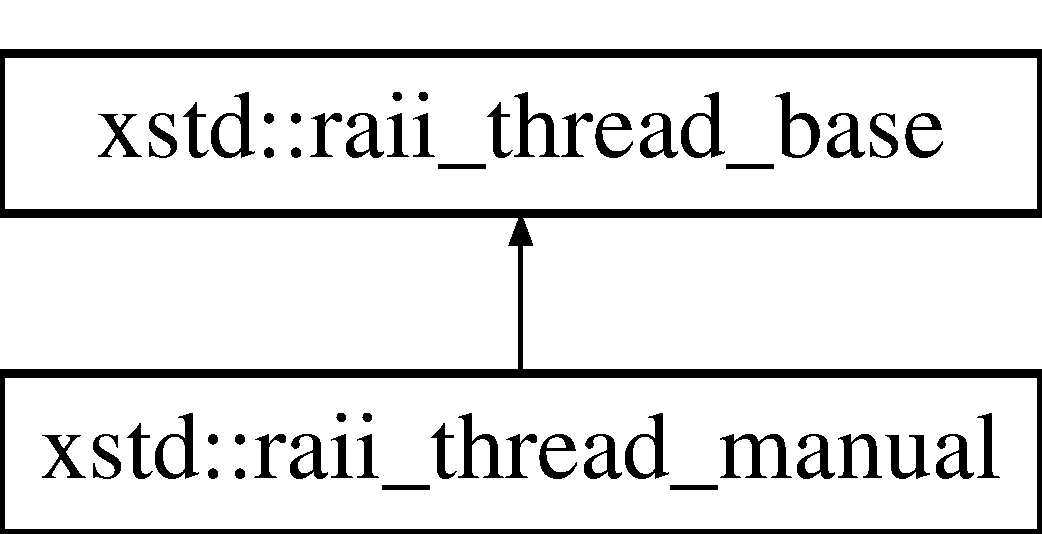
\includegraphics[height=2.000000cm]{classxstd_1_1raii__thread__manual}
\end{center}
\end{figure}
\subsection*{Public Member Functions}
\begin{DoxyCompactItemize}
\item 
\hypertarget{classxstd_1_1raii__thread__manual_a7a6c9e815d104ba820b3deaa5eef4000}{{\bfseries raii\-\_\-thread\-\_\-manual} (std\-::function$<$ void()$>$ client\-\_\-routine)}\label{classxstd_1_1raii__thread__manual_a7a6c9e815d104ba820b3deaa5eef4000}

\item 
\hypertarget{classxstd_1_1raii__thread__manual_a4998457f902ae8515ba0a37a8c78e37a}{void {\bfseries start} (void)}\label{classxstd_1_1raii__thread__manual_a4998457f902ae8515ba0a37a8c78e37a}

\item 
\hypertarget{classxstd_1_1raii__thread__manual_a00dc2a5fc7895b700a88afcdb9fa0f23}{void {\bfseries stop} (void)}\label{classxstd_1_1raii__thread__manual_a00dc2a5fc7895b700a88afcdb9fa0f23}

\end{DoxyCompactItemize}
\subsection*{Additional Inherited Members}


The documentation for this class was generated from the following files\-:\begin{DoxyCompactItemize}
\item 
src/thread/raii\-\_\-thread\-\_\-manual/src/raii\-\_\-thread\-\_\-manual.\-hpp\item 
src/thread/raii\-\_\-thread\-\_\-manual/src/raii\-\_\-thread\-\_\-manual.\-ipp\end{DoxyCompactItemize}

\hypertarget{classxstd_1_1chrono_1_1timer}{\section{xstd\-:\-:chrono\-:\-:timer$<$ clock $>$ Class Template Reference}
\label{classxstd_1_1chrono_1_1timer}\index{xstd\-::chrono\-::timer$<$ clock $>$@{xstd\-::chrono\-::timer$<$ clock $>$}}
}


{\ttfamily \#include $<$timer.\-hpp$>$}

Inheritance diagram for xstd\-:\-:chrono\-:\-:timer$<$ clock $>$\-:\begin{figure}[H]
\begin{center}
\leavevmode
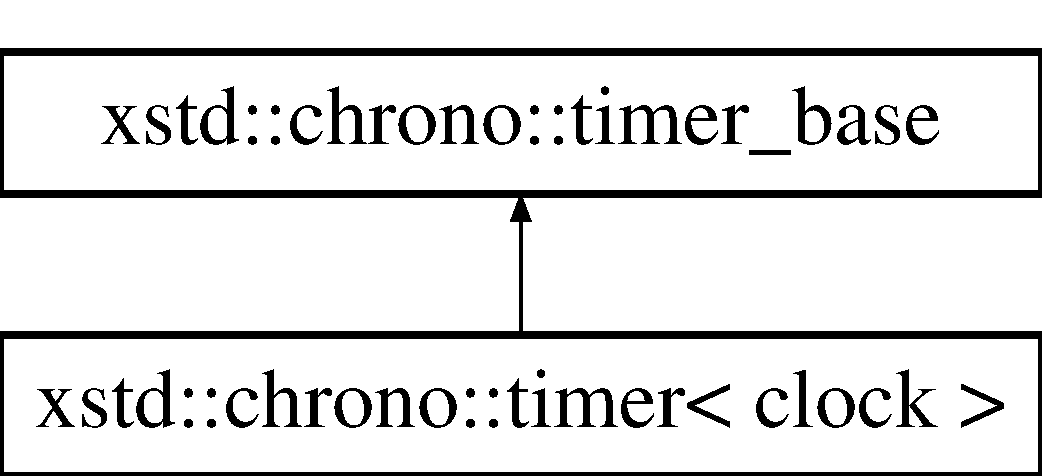
\includegraphics[height=2.000000cm]{classxstd_1_1chrono_1_1timer}
\end{center}
\end{figure}
\subsection*{Public Member Functions}
\begin{DoxyCompactItemize}
\item 
\hyperlink{classxstd_1_1chrono_1_1timer_a1d151d2452b9a4b5d00b37b238b86a9c}{timer} (void)
\item 
virtual \hyperlink{classxstd_1_1chrono_1_1timer_a274db25436fb2392246f64395ac4f2dc}{$\sim$timer} (void) noexcept
\item 
bool \hyperlink{classxstd_1_1chrono_1_1timer_a1496749b90d70cee8c29c66f9c67e21a}{get\-\_\-is\-\_\-active} (void) const 
\item 
void \hyperlink{classxstd_1_1chrono_1_1timer_a6ad3088df2f2ca33ea7246f1c716b65a}{get\-\_\-ticks\-\_\-done} (void) const 
\item 
void \hyperlink{classxstd_1_1chrono_1_1timer_a66a27994093e3a8cd5be70e82e577e25}{start} (void)
\item 
void \hyperlink{classxstd_1_1chrono_1_1timer_acb361a9fbbafe351513ee6251feb1000}{stop} (void)
\end{DoxyCompactItemize}
\subsection*{Public Attributes}
\begin{DoxyCompactItemize}
\item 
duration \hyperlink{classxstd_1_1chrono_1_1timer_a57838b4d220986131fcd8f5ddc1363bc}{tick\-\_\-interval}
\item 
unsigned int \hyperlink{classxstd_1_1chrono_1_1timer_a68ac37affa234daf952955ab2c1d674e}{tick\-\_\-limit}
\item 
event\-\_\-start\-\_\-type \hyperlink{classxstd_1_1chrono_1_1timer_acd6563ae4202b5d67856562d5a024894}{event\-\_\-start}
\item 
event\-\_\-tick\-\_\-type \hyperlink{classxstd_1_1chrono_1_1timer_a7bfca0bacd30aabd2bf7a69e25f2574c}{event\-\_\-tick}
\item 
event\-\_\-complete\-\_\-type \hyperlink{classxstd_1_1chrono_1_1timer_ac12f83ed705997b32c1dcf8853cf93c9}{event\-\_\-complete}
\item 
event\-\_\-stop\-\_\-type \hyperlink{classxstd_1_1chrono_1_1timer_a2f14e4ebe72f6c127f564f2dc4e97909}{event\-\_\-stop}
\end{DoxyCompactItemize}
\subsection*{Protected Member Functions}
\begin{DoxyCompactItemize}
\item 
bool \hyperlink{classxstd_1_1chrono_1_1timer_a79c070e4f1be92f8d8cf0cb62ebe0b2c}{requires\-\_\-tick} (void)
\item 
virtual void \hyperlink{classxstd_1_1chrono_1_1timer_a587e45f1e39ab87de14cda6f39e713da}{tick} (void) override
\item 
void \hyperlink{classxstd_1_1chrono_1_1timer_aef7b4094eebf22027987e81993859488}{update\-\_\-next\-\_\-tick\-\_\-time\-\_\-point} (void)
\item 
void \hyperlink{classxstd_1_1chrono_1_1timer_a6088ae4c5a93946c1159122305d76535}{check\-\_\-is\-\_\-ready\-\_\-to\-\_\-start} (void) const 
\item 
void \hyperlink{classxstd_1_1chrono_1_1timer_a631105f997839a66fb79c7ff87d83532}{check\-\_\-is\-\_\-ready\-\_\-to\-\_\-stop} (void) const 
\end{DoxyCompactItemize}
\subsection*{Protected Attributes}
\begin{DoxyCompactItemize}
\item 
bool \hyperlink{classxstd_1_1chrono_1_1timer_ac6a3c41d433b7e1387c297b925fb26d7}{is\-\_\-active}
\item 
unsigned int \hyperlink{classxstd_1_1chrono_1_1timer_a40ec5c890d4e54669729744b634daa9e}{ticks\-\_\-done}
\item 
time\-\_\-point \hyperlink{classxstd_1_1chrono_1_1timer_a51e85ae6c2a43cef074e5ff3e03620f9}{next\-\_\-tick\-\_\-time\-\_\-point}
\end{DoxyCompactItemize}


\subsection{Constructor \& Destructor Documentation}
\hypertarget{classxstd_1_1chrono_1_1timer_a1d151d2452b9a4b5d00b37b238b86a9c}{\index{xstd\-::chrono\-::timer@{xstd\-::chrono\-::timer}!timer@{timer}}
\index{timer@{timer}!xstd::chrono::timer@{xstd\-::chrono\-::timer}}
\subsubsection[{timer}]{\setlength{\rightskip}{0pt plus 5cm}template$<$typename clock  = std\-::chrono\-::high\-\_\-resolution\-\_\-clock$>$ {\bf xstd\-::chrono\-::timer}$<$ clock $>$\-::{\bf timer} (
\begin{DoxyParamCaption}
\item[{void}]{}
\end{DoxyParamCaption}
)\hspace{0.3cm}{\ttfamily [inline]}, {\ttfamily [explicit]}}}\label{classxstd_1_1chrono_1_1timer_a1d151d2452b9a4b5d00b37b238b86a9c}
\hypertarget{classxstd_1_1chrono_1_1timer_a274db25436fb2392246f64395ac4f2dc}{\index{xstd\-::chrono\-::timer@{xstd\-::chrono\-::timer}!$\sim$timer@{$\sim$timer}}
\index{$\sim$timer@{$\sim$timer}!xstd::chrono::timer@{xstd\-::chrono\-::timer}}
\subsubsection[{$\sim$timer}]{\setlength{\rightskip}{0pt plus 5cm}template$<$typename clock  = std\-::chrono\-::high\-\_\-resolution\-\_\-clock$>$ virtual {\bf xstd\-::chrono\-::timer}$<$ clock $>$\-::$\sim${\bf timer} (
\begin{DoxyParamCaption}
\item[{void}]{}
\end{DoxyParamCaption}
)\hspace{0.3cm}{\ttfamily [inline]}, {\ttfamily [virtual]}}}\label{classxstd_1_1chrono_1_1timer_a274db25436fb2392246f64395ac4f2dc}


\subsection{Member Function Documentation}
\hypertarget{classxstd_1_1chrono_1_1timer_a6088ae4c5a93946c1159122305d76535}{\index{xstd\-::chrono\-::timer@{xstd\-::chrono\-::timer}!check\-\_\-is\-\_\-ready\-\_\-to\-\_\-start@{check\-\_\-is\-\_\-ready\-\_\-to\-\_\-start}}
\index{check\-\_\-is\-\_\-ready\-\_\-to\-\_\-start@{check\-\_\-is\-\_\-ready\-\_\-to\-\_\-start}!xstd::chrono::timer@{xstd\-::chrono\-::timer}}
\subsubsection[{check\-\_\-is\-\_\-ready\-\_\-to\-\_\-start}]{\setlength{\rightskip}{0pt plus 5cm}template$<$typename clock  = std\-::chrono\-::high\-\_\-resolution\-\_\-clock$>$ void {\bf xstd\-::chrono\-::timer}$<$ clock $>$\-::check\-\_\-is\-\_\-ready\-\_\-to\-\_\-start (
\begin{DoxyParamCaption}
\item[{void}]{}
\end{DoxyParamCaption}
) const\hspace{0.3cm}{\ttfamily [inline]}, {\ttfamily [protected]}}}\label{classxstd_1_1chrono_1_1timer_a6088ae4c5a93946c1159122305d76535}
\hypertarget{classxstd_1_1chrono_1_1timer_a631105f997839a66fb79c7ff87d83532}{\index{xstd\-::chrono\-::timer@{xstd\-::chrono\-::timer}!check\-\_\-is\-\_\-ready\-\_\-to\-\_\-stop@{check\-\_\-is\-\_\-ready\-\_\-to\-\_\-stop}}
\index{check\-\_\-is\-\_\-ready\-\_\-to\-\_\-stop@{check\-\_\-is\-\_\-ready\-\_\-to\-\_\-stop}!xstd::chrono::timer@{xstd\-::chrono\-::timer}}
\subsubsection[{check\-\_\-is\-\_\-ready\-\_\-to\-\_\-stop}]{\setlength{\rightskip}{0pt plus 5cm}template$<$typename clock  = std\-::chrono\-::high\-\_\-resolution\-\_\-clock$>$ void {\bf xstd\-::chrono\-::timer}$<$ clock $>$\-::check\-\_\-is\-\_\-ready\-\_\-to\-\_\-stop (
\begin{DoxyParamCaption}
\item[{void}]{}
\end{DoxyParamCaption}
) const\hspace{0.3cm}{\ttfamily [inline]}, {\ttfamily [protected]}}}\label{classxstd_1_1chrono_1_1timer_a631105f997839a66fb79c7ff87d83532}
\hypertarget{classxstd_1_1chrono_1_1timer_a1496749b90d70cee8c29c66f9c67e21a}{\index{xstd\-::chrono\-::timer@{xstd\-::chrono\-::timer}!get\-\_\-is\-\_\-active@{get\-\_\-is\-\_\-active}}
\index{get\-\_\-is\-\_\-active@{get\-\_\-is\-\_\-active}!xstd::chrono::timer@{xstd\-::chrono\-::timer}}
\subsubsection[{get\-\_\-is\-\_\-active}]{\setlength{\rightskip}{0pt plus 5cm}template$<$typename clock  = std\-::chrono\-::high\-\_\-resolution\-\_\-clock$>$ bool {\bf xstd\-::chrono\-::timer}$<$ clock $>$\-::get\-\_\-is\-\_\-active (
\begin{DoxyParamCaption}
\item[{void}]{}
\end{DoxyParamCaption}
) const\hspace{0.3cm}{\ttfamily [inline]}}}\label{classxstd_1_1chrono_1_1timer_a1496749b90d70cee8c29c66f9c67e21a}
\hypertarget{classxstd_1_1chrono_1_1timer_a6ad3088df2f2ca33ea7246f1c716b65a}{\index{xstd\-::chrono\-::timer@{xstd\-::chrono\-::timer}!get\-\_\-ticks\-\_\-done@{get\-\_\-ticks\-\_\-done}}
\index{get\-\_\-ticks\-\_\-done@{get\-\_\-ticks\-\_\-done}!xstd::chrono::timer@{xstd\-::chrono\-::timer}}
\subsubsection[{get\-\_\-ticks\-\_\-done}]{\setlength{\rightskip}{0pt plus 5cm}template$<$typename clock  = std\-::chrono\-::high\-\_\-resolution\-\_\-clock$>$ void {\bf xstd\-::chrono\-::timer}$<$ clock $>$\-::get\-\_\-ticks\-\_\-done (
\begin{DoxyParamCaption}
\item[{void}]{}
\end{DoxyParamCaption}
) const\hspace{0.3cm}{\ttfamily [inline]}}}\label{classxstd_1_1chrono_1_1timer_a6ad3088df2f2ca33ea7246f1c716b65a}
\hypertarget{classxstd_1_1chrono_1_1timer_a79c070e4f1be92f8d8cf0cb62ebe0b2c}{\index{xstd\-::chrono\-::timer@{xstd\-::chrono\-::timer}!requires\-\_\-tick@{requires\-\_\-tick}}
\index{requires\-\_\-tick@{requires\-\_\-tick}!xstd::chrono::timer@{xstd\-::chrono\-::timer}}
\subsubsection[{requires\-\_\-tick}]{\setlength{\rightskip}{0pt plus 5cm}template$<$typename clock  = std\-::chrono\-::high\-\_\-resolution\-\_\-clock$>$ bool {\bf xstd\-::chrono\-::timer}$<$ clock $>$\-::requires\-\_\-tick (
\begin{DoxyParamCaption}
\item[{void}]{}
\end{DoxyParamCaption}
)\hspace{0.3cm}{\ttfamily [inline]}, {\ttfamily [protected]}}}\label{classxstd_1_1chrono_1_1timer_a79c070e4f1be92f8d8cf0cb62ebe0b2c}
\hypertarget{classxstd_1_1chrono_1_1timer_a66a27994093e3a8cd5be70e82e577e25}{\index{xstd\-::chrono\-::timer@{xstd\-::chrono\-::timer}!start@{start}}
\index{start@{start}!xstd::chrono::timer@{xstd\-::chrono\-::timer}}
\subsubsection[{start}]{\setlength{\rightskip}{0pt plus 5cm}template$<$typename clock  = std\-::chrono\-::high\-\_\-resolution\-\_\-clock$>$ void {\bf xstd\-::chrono\-::timer}$<$ clock $>$\-::start (
\begin{DoxyParamCaption}
\item[{void}]{}
\end{DoxyParamCaption}
)\hspace{0.3cm}{\ttfamily [inline]}}}\label{classxstd_1_1chrono_1_1timer_a66a27994093e3a8cd5be70e82e577e25}
\hypertarget{classxstd_1_1chrono_1_1timer_acb361a9fbbafe351513ee6251feb1000}{\index{xstd\-::chrono\-::timer@{xstd\-::chrono\-::timer}!stop@{stop}}
\index{stop@{stop}!xstd::chrono::timer@{xstd\-::chrono\-::timer}}
\subsubsection[{stop}]{\setlength{\rightskip}{0pt plus 5cm}template$<$typename clock  = std\-::chrono\-::high\-\_\-resolution\-\_\-clock$>$ void {\bf xstd\-::chrono\-::timer}$<$ clock $>$\-::stop (
\begin{DoxyParamCaption}
\item[{void}]{}
\end{DoxyParamCaption}
)\hspace{0.3cm}{\ttfamily [inline]}}}\label{classxstd_1_1chrono_1_1timer_acb361a9fbbafe351513ee6251feb1000}
\hypertarget{classxstd_1_1chrono_1_1timer_a587e45f1e39ab87de14cda6f39e713da}{\index{xstd\-::chrono\-::timer@{xstd\-::chrono\-::timer}!tick@{tick}}
\index{tick@{tick}!xstd::chrono::timer@{xstd\-::chrono\-::timer}}
\subsubsection[{tick}]{\setlength{\rightskip}{0pt plus 5cm}template$<$typename clock  = std\-::chrono\-::high\-\_\-resolution\-\_\-clock$>$ virtual void {\bf xstd\-::chrono\-::timer}$<$ clock $>$\-::tick (
\begin{DoxyParamCaption}
\item[{void}]{}
\end{DoxyParamCaption}
)\hspace{0.3cm}{\ttfamily [inline]}, {\ttfamily [override]}, {\ttfamily [protected]}, {\ttfamily [virtual]}}}\label{classxstd_1_1chrono_1_1timer_a587e45f1e39ab87de14cda6f39e713da}


Implements \hyperlink{classxstd_1_1chrono_1_1timer__base_a2d7c36af22ff593ca31849531fe23fd8}{xstd\-::chrono\-::timer\-\_\-base}.

\hypertarget{classxstd_1_1chrono_1_1timer_aef7b4094eebf22027987e81993859488}{\index{xstd\-::chrono\-::timer@{xstd\-::chrono\-::timer}!update\-\_\-next\-\_\-tick\-\_\-time\-\_\-point@{update\-\_\-next\-\_\-tick\-\_\-time\-\_\-point}}
\index{update\-\_\-next\-\_\-tick\-\_\-time\-\_\-point@{update\-\_\-next\-\_\-tick\-\_\-time\-\_\-point}!xstd::chrono::timer@{xstd\-::chrono\-::timer}}
\subsubsection[{update\-\_\-next\-\_\-tick\-\_\-time\-\_\-point}]{\setlength{\rightskip}{0pt plus 5cm}template$<$typename clock  = std\-::chrono\-::high\-\_\-resolution\-\_\-clock$>$ void {\bf xstd\-::chrono\-::timer}$<$ clock $>$\-::update\-\_\-next\-\_\-tick\-\_\-time\-\_\-point (
\begin{DoxyParamCaption}
\item[{void}]{}
\end{DoxyParamCaption}
)\hspace{0.3cm}{\ttfamily [inline]}, {\ttfamily [protected]}}}\label{classxstd_1_1chrono_1_1timer_aef7b4094eebf22027987e81993859488}


\subsection{Member Data Documentation}
\hypertarget{classxstd_1_1chrono_1_1timer_ac12f83ed705997b32c1dcf8853cf93c9}{\index{xstd\-::chrono\-::timer@{xstd\-::chrono\-::timer}!event\-\_\-complete@{event\-\_\-complete}}
\index{event\-\_\-complete@{event\-\_\-complete}!xstd::chrono::timer@{xstd\-::chrono\-::timer}}
\subsubsection[{event\-\_\-complete}]{\setlength{\rightskip}{0pt plus 5cm}template$<$typename clock  = std\-::chrono\-::high\-\_\-resolution\-\_\-clock$>$ event\-\_\-complete\-\_\-type {\bf xstd\-::chrono\-::timer}$<$ clock $>$\-::event\-\_\-complete}}\label{classxstd_1_1chrono_1_1timer_ac12f83ed705997b32c1dcf8853cf93c9}
\hypertarget{classxstd_1_1chrono_1_1timer_acd6563ae4202b5d67856562d5a024894}{\index{xstd\-::chrono\-::timer@{xstd\-::chrono\-::timer}!event\-\_\-start@{event\-\_\-start}}
\index{event\-\_\-start@{event\-\_\-start}!xstd::chrono::timer@{xstd\-::chrono\-::timer}}
\subsubsection[{event\-\_\-start}]{\setlength{\rightskip}{0pt plus 5cm}template$<$typename clock  = std\-::chrono\-::high\-\_\-resolution\-\_\-clock$>$ event\-\_\-start\-\_\-type {\bf xstd\-::chrono\-::timer}$<$ clock $>$\-::event\-\_\-start}}\label{classxstd_1_1chrono_1_1timer_acd6563ae4202b5d67856562d5a024894}
\hypertarget{classxstd_1_1chrono_1_1timer_a2f14e4ebe72f6c127f564f2dc4e97909}{\index{xstd\-::chrono\-::timer@{xstd\-::chrono\-::timer}!event\-\_\-stop@{event\-\_\-stop}}
\index{event\-\_\-stop@{event\-\_\-stop}!xstd::chrono::timer@{xstd\-::chrono\-::timer}}
\subsubsection[{event\-\_\-stop}]{\setlength{\rightskip}{0pt plus 5cm}template$<$typename clock  = std\-::chrono\-::high\-\_\-resolution\-\_\-clock$>$ event\-\_\-stop\-\_\-type {\bf xstd\-::chrono\-::timer}$<$ clock $>$\-::event\-\_\-stop}}\label{classxstd_1_1chrono_1_1timer_a2f14e4ebe72f6c127f564f2dc4e97909}
\hypertarget{classxstd_1_1chrono_1_1timer_a7bfca0bacd30aabd2bf7a69e25f2574c}{\index{xstd\-::chrono\-::timer@{xstd\-::chrono\-::timer}!event\-\_\-tick@{event\-\_\-tick}}
\index{event\-\_\-tick@{event\-\_\-tick}!xstd::chrono::timer@{xstd\-::chrono\-::timer}}
\subsubsection[{event\-\_\-tick}]{\setlength{\rightskip}{0pt plus 5cm}template$<$typename clock  = std\-::chrono\-::high\-\_\-resolution\-\_\-clock$>$ event\-\_\-tick\-\_\-type {\bf xstd\-::chrono\-::timer}$<$ clock $>$\-::event\-\_\-tick}}\label{classxstd_1_1chrono_1_1timer_a7bfca0bacd30aabd2bf7a69e25f2574c}
\hypertarget{classxstd_1_1chrono_1_1timer_ac6a3c41d433b7e1387c297b925fb26d7}{\index{xstd\-::chrono\-::timer@{xstd\-::chrono\-::timer}!is\-\_\-active@{is\-\_\-active}}
\index{is\-\_\-active@{is\-\_\-active}!xstd::chrono::timer@{xstd\-::chrono\-::timer}}
\subsubsection[{is\-\_\-active}]{\setlength{\rightskip}{0pt plus 5cm}template$<$typename clock  = std\-::chrono\-::high\-\_\-resolution\-\_\-clock$>$ bool {\bf xstd\-::chrono\-::timer}$<$ clock $>$\-::is\-\_\-active\hspace{0.3cm}{\ttfamily [protected]}}}\label{classxstd_1_1chrono_1_1timer_ac6a3c41d433b7e1387c297b925fb26d7}
\hypertarget{classxstd_1_1chrono_1_1timer_a51e85ae6c2a43cef074e5ff3e03620f9}{\index{xstd\-::chrono\-::timer@{xstd\-::chrono\-::timer}!next\-\_\-tick\-\_\-time\-\_\-point@{next\-\_\-tick\-\_\-time\-\_\-point}}
\index{next\-\_\-tick\-\_\-time\-\_\-point@{next\-\_\-tick\-\_\-time\-\_\-point}!xstd::chrono::timer@{xstd\-::chrono\-::timer}}
\subsubsection[{next\-\_\-tick\-\_\-time\-\_\-point}]{\setlength{\rightskip}{0pt plus 5cm}template$<$typename clock  = std\-::chrono\-::high\-\_\-resolution\-\_\-clock$>$ time\-\_\-point {\bf xstd\-::chrono\-::timer}$<$ clock $>$\-::next\-\_\-tick\-\_\-time\-\_\-point\hspace{0.3cm}{\ttfamily [protected]}}}\label{classxstd_1_1chrono_1_1timer_a51e85ae6c2a43cef074e5ff3e03620f9}
\hypertarget{classxstd_1_1chrono_1_1timer_a57838b4d220986131fcd8f5ddc1363bc}{\index{xstd\-::chrono\-::timer@{xstd\-::chrono\-::timer}!tick\-\_\-interval@{tick\-\_\-interval}}
\index{tick\-\_\-interval@{tick\-\_\-interval}!xstd::chrono::timer@{xstd\-::chrono\-::timer}}
\subsubsection[{tick\-\_\-interval}]{\setlength{\rightskip}{0pt plus 5cm}template$<$typename clock  = std\-::chrono\-::high\-\_\-resolution\-\_\-clock$>$ duration {\bf xstd\-::chrono\-::timer}$<$ clock $>$\-::tick\-\_\-interval}}\label{classxstd_1_1chrono_1_1timer_a57838b4d220986131fcd8f5ddc1363bc}
\hypertarget{classxstd_1_1chrono_1_1timer_a68ac37affa234daf952955ab2c1d674e}{\index{xstd\-::chrono\-::timer@{xstd\-::chrono\-::timer}!tick\-\_\-limit@{tick\-\_\-limit}}
\index{tick\-\_\-limit@{tick\-\_\-limit}!xstd::chrono::timer@{xstd\-::chrono\-::timer}}
\subsubsection[{tick\-\_\-limit}]{\setlength{\rightskip}{0pt plus 5cm}template$<$typename clock  = std\-::chrono\-::high\-\_\-resolution\-\_\-clock$>$ unsigned int {\bf xstd\-::chrono\-::timer}$<$ clock $>$\-::tick\-\_\-limit}}\label{classxstd_1_1chrono_1_1timer_a68ac37affa234daf952955ab2c1d674e}
\hypertarget{classxstd_1_1chrono_1_1timer_a40ec5c890d4e54669729744b634daa9e}{\index{xstd\-::chrono\-::timer@{xstd\-::chrono\-::timer}!ticks\-\_\-done@{ticks\-\_\-done}}
\index{ticks\-\_\-done@{ticks\-\_\-done}!xstd::chrono::timer@{xstd\-::chrono\-::timer}}
\subsubsection[{ticks\-\_\-done}]{\setlength{\rightskip}{0pt plus 5cm}template$<$typename clock  = std\-::chrono\-::high\-\_\-resolution\-\_\-clock$>$ unsigned int {\bf xstd\-::chrono\-::timer}$<$ clock $>$\-::ticks\-\_\-done\hspace{0.3cm}{\ttfamily [protected]}}}\label{classxstd_1_1chrono_1_1timer_a40ec5c890d4e54669729744b634daa9e}


The documentation for this class was generated from the following file\-:\begin{DoxyCompactItemize}
\item 
src/chrono/timer/timer/src/\hyperlink{timer_8hpp}{timer.\-hpp}\end{DoxyCompactItemize}

\hypertarget{classxstd_1_1chrono_1_1timer__base}{\section{xstd\-:\-:chrono\-:\-:timer\-\_\-base Class Reference}
\label{classxstd_1_1chrono_1_1timer__base}\index{xstd\-::chrono\-::timer\-\_\-base@{xstd\-::chrono\-::timer\-\_\-base}}
}
Inheritance diagram for xstd\-:\-:chrono\-:\-:timer\-\_\-base\-:\begin{figure}[H]
\begin{center}
\leavevmode
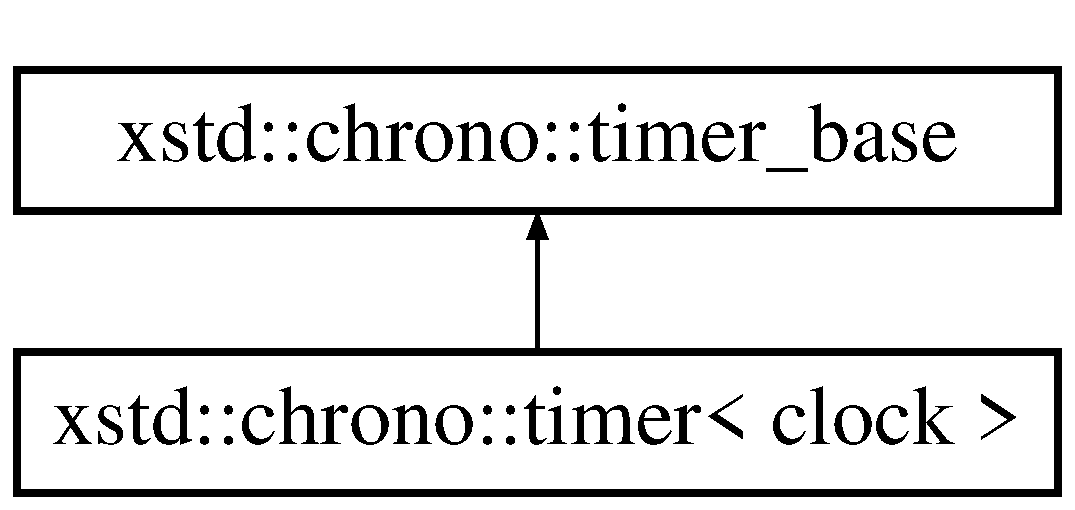
\includegraphics[height=2.000000cm]{classxstd_1_1chrono_1_1timer__base}
\end{center}
\end{figure}
\subsection*{Public Member Functions}
\begin{DoxyCompactItemize}
\item 
\hypertarget{classxstd_1_1chrono_1_1timer__base_a2d7c36af22ff593ca31849531fe23fd8}{virtual void {\bfseries tick} (void)=0}\label{classxstd_1_1chrono_1_1timer__base_a2d7c36af22ff593ca31849531fe23fd8}

\end{DoxyCompactItemize}


The documentation for this class was generated from the following file\-:\begin{DoxyCompactItemize}
\item 
src/chrono/timer/timer\-\_\-base/src/timer\-\_\-base.\-hpp\end{DoxyCompactItemize}

\hypertarget{classxstd_1_1chrono_1_1timer__manager}{\section{xstd\-:\-:chrono\-:\-:timer\-\_\-manager Class Reference}
\label{classxstd_1_1chrono_1_1timer__manager}\index{xstd\-::chrono\-::timer\-\_\-manager@{xstd\-::chrono\-::timer\-\_\-manager}}
}
\subsection*{Public Member Functions}
\begin{DoxyCompactItemize}
\item 
\hypertarget{classxstd_1_1chrono_1_1timer__manager_ae97c0dba8154bace5af93caae4948c8c}{void {\bfseries add\-\_\-timer} (\hyperlink{classxstd_1_1chrono_1_1timer__base}{timer\-\_\-base} $\ast$const timer\-\_\-ptr)}\label{classxstd_1_1chrono_1_1timer__manager_ae97c0dba8154bace5af93caae4948c8c}

\item 
\hypertarget{classxstd_1_1chrono_1_1timer__manager_af368bd572a757f8f78e39e4572114a84}{void {\bfseries remove\-\_\-timer} (\hyperlink{classxstd_1_1chrono_1_1timer__base}{timer\-\_\-base} $\ast$const timer\-\_\-ptr)}\label{classxstd_1_1chrono_1_1timer__manager_af368bd572a757f8f78e39e4572114a84}

\end{DoxyCompactItemize}
\subsection*{Static Public Member Functions}
\begin{DoxyCompactItemize}
\item 
\hypertarget{classxstd_1_1chrono_1_1timer__manager_a8894928f093db753153f2f87dfa511e0}{static \hyperlink{classxstd_1_1chrono_1_1timer__manager}{timer\-\_\-manager} \& {\bfseries get\-\_\-instance} (void)}\label{classxstd_1_1chrono_1_1timer__manager_a8894928f093db753153f2f87dfa511e0}

\end{DoxyCompactItemize}


The documentation for this class was generated from the following file\-:\begin{DoxyCompactItemize}
\item 
src/chrono/timer/timer\-\_\-manager/src/timer\-\_\-manager.\-hpp\end{DoxyCompactItemize}

\chapter{File Documentation}
\hypertarget{chrono__util_8hpp}{\section{src/chrono/chrono\-\_\-util/src/chrono\-\_\-util.hpp File Reference}
\label{chrono__util_8hpp}\index{src/chrono/chrono\-\_\-util/src/chrono\-\_\-util.\-hpp@{src/chrono/chrono\-\_\-util/src/chrono\-\_\-util.\-hpp}}
}
{\ttfamily \#include $<$stdexcept$>$}\\*
{\ttfamily \#include $<$chrono$>$}\\*
{\ttfamily \#include $<$ctime$>$}\\*
{\ttfamily \#include $<$string$>$}\\*
{\ttfamily \#include $<$mutex$>$}\\*
{\ttfamily \#include \char`\"{}chrono\-\_\-util.\-ipp\char`\"{}}\\*
\subsection*{Namespaces}
\begin{DoxyCompactItemize}
\item 
namespace \hyperlink{namespacexstd}{xstd}
\item 
namespace \hyperlink{namespacexstd_1_1chrono}{xstd\-::chrono}
\end{DoxyCompactItemize}
\subsection*{Functions}
\begin{DoxyCompactItemize}
\item 
time\-\_\-t \hyperlink{namespacexstd_1_1chrono_af3f86d799ca227d2bf0ac8ff5a08df3b}{xstd\-::chrono\-::time\-\_\-point\-\_\-to\-\_\-time\-\_\-t} (const std\-::chrono\-::time\-\_\-point$<$ std\-::chrono\-::steady\-\_\-clock $>$ \&time\-\_\-point)
\item 
tm \hyperlink{namespacexstd_1_1chrono_a1f31cb15f2e74489fc0f98fa38758067}{xstd\-::chrono\-::time\-\_\-point\-\_\-to\-\_\-tm} (const std\-::chrono\-::time\-\_\-point$<$ std\-::chrono\-::steady\-\_\-clock $>$ \&time\-\_\-point)
\item 
std\-::string \hyperlink{namespacexstd_1_1chrono_a5fd95ee0963d407c39528b3f48790842}{xstd\-::chrono\-::time\-\_\-point\-\_\-to\-\_\-formatted\-\_\-string} (const std\-::chrono\-::time\-\_\-point$<$ std\-::chrono\-::steady\-\_\-clock $>$ \&time\-\_\-point, const std\-::string \&time\-\_\-format=\char`\"{}\mbox{[}\%Y/\%m/\%d-\/\%H\-:\%M\-:\%S\mbox{]}\char`\"{})
\item 
std\-::string \hyperlink{namespacexstd_1_1chrono_a07cd40fda33f294f91510fe6895ce6c7}{xstd\-::chrono\-::time\-\_\-point\-\_\-to\-\_\-formatted\-\_\-string\-\_\-mt} (const std\-::chrono\-::time\-\_\-point$<$ std\-::chrono\-::steady\-\_\-clock $>$ \&time\-\_\-point, const std\-::string \&time\-\_\-format=\char`\"{}\mbox{[}\%Y/\%m/\%d-\/\%H\-:\%M\-:\%S\mbox{]}\char`\"{})
\end{DoxyCompactItemize}

\hypertarget{chrono__util_8ipp}{\section{src/chrono/chrono\-\_\-util/src/chrono\-\_\-util.ipp File Reference}
\label{chrono__util_8ipp}\index{src/chrono/chrono\-\_\-util/src/chrono\-\_\-util.\-ipp@{src/chrono/chrono\-\_\-util/src/chrono\-\_\-util.\-ipp}}
}
\subsection*{Namespaces}
\begin{DoxyCompactItemize}
\item 
namespace \hyperlink{namespacexstd}{xstd}
\item 
namespace \hyperlink{namespacexstd_1_1chrono}{xstd\-::chrono}
\end{DoxyCompactItemize}
\subsection*{Functions}
\begin{DoxyCompactItemize}
\item 
time\-\_\-t \hyperlink{namespacexstd_1_1chrono_af3f86d799ca227d2bf0ac8ff5a08df3b}{xstd\-::chrono\-::time\-\_\-point\-\_\-to\-\_\-time\-\_\-t} (const std\-::chrono\-::time\-\_\-point$<$ std\-::chrono\-::steady\-\_\-clock $>$ \&time\-\_\-point)
\item 
tm \hyperlink{namespacexstd_1_1chrono_a1f31cb15f2e74489fc0f98fa38758067}{xstd\-::chrono\-::time\-\_\-point\-\_\-to\-\_\-tm} (const std\-::chrono\-::time\-\_\-point$<$ std\-::chrono\-::steady\-\_\-clock $>$ \&time\-\_\-point)
\item 
std\-::string \hyperlink{namespacexstd_1_1chrono_a5fd95ee0963d407c39528b3f48790842}{xstd\-::chrono\-::time\-\_\-point\-\_\-to\-\_\-formatted\-\_\-string} (const std\-::chrono\-::time\-\_\-point$<$ std\-::chrono\-::steady\-\_\-clock $>$ \&time\-\_\-point, const std\-::string \&time\-\_\-format=\char`\"{}\mbox{[}\%Y/\%m/\%d-\/\%H\-:\%M\-:\%S\mbox{]}\char`\"{})
\item 
std\-::string \hyperlink{namespacexstd_1_1chrono_a07cd40fda33f294f91510fe6895ce6c7}{xstd\-::chrono\-::time\-\_\-point\-\_\-to\-\_\-formatted\-\_\-string\-\_\-mt} (const std\-::chrono\-::time\-\_\-point$<$ std\-::chrono\-::steady\-\_\-clock $>$ \&time\-\_\-point, const std\-::string \&time\-\_\-format=\char`\"{}\mbox{[}\%Y/\%m/\%d-\/\%H\-:\%M\-:\%S\mbox{]}\char`\"{})
\end{DoxyCompactItemize}

\hypertarget{chrono__util__tests_8cpp}{\section{src/chrono/chrono\-\_\-util/tests/src/chrono\-\_\-util\-\_\-tests.cpp File Reference}
\label{chrono__util__tests_8cpp}\index{src/chrono/chrono\-\_\-util/tests/src/chrono\-\_\-util\-\_\-tests.\-cpp@{src/chrono/chrono\-\_\-util/tests/src/chrono\-\_\-util\-\_\-tests.\-cpp}}
}
{\ttfamily \#include $<$gtest/gtest.\-h$>$}\\*
{\ttfamily \#include $<$cstring$>$}\\*
{\ttfamily \#include $<$chrono/chrono\-\_\-util.\-hpp$>$}\\*
\subsection*{Functions}
\begin{DoxyCompactItemize}
\item 
\hyperlink{chrono__util__tests_8cpp_a4d515f066f202870d93427c6823ebeca}{T\-E\-S\-T} (one\-\_\-second\-\_\-time\-\_\-point, converts\-\_\-to\-\_\-time\-\_\-t\-\_\-equal\-\_\-to\-\_\-1)
\item 
\hyperlink{chrono__util__tests_8cpp_a69c5ff47696ea16358cdd6057cf7bf17}{T\-E\-S\-T} (one\-\_\-second\-\_\-time\-\_\-point, converts\-\_\-to\-\_\-string\-\_\-1970\-\_\-01\-\_\-01\-\_\-00\-\_\-00\-\_\-01)
\item 
\hyperlink{chrono__util__tests_8cpp_a4a87b4ecd178fc6214a468487a23b311}{T\-E\-S\-T} (one\-\_\-minute\-\_\-time\-\_\-point, converts\-\_\-to\-\_\-time\-\_\-t\-\_\-equal\-\_\-to\-\_\-60)
\item 
\hyperlink{chrono__util__tests_8cpp_ae6f833f88a5feb486514bc6c944df7a4}{T\-E\-S\-T} (one\-\_\-minute\-\_\-time\-\_\-point, converts\-\_\-to\-\_\-equal\-\_\-tm)
\item 
\hyperlink{chrono__util__tests_8cpp_a2e5964195ce539f6196eeb962b1b5b84}{T\-E\-S\-T} (one\-\_\-hour\-\_\-time\-\_\-point, converts\-\_\-to\-\_\-time\-\_\-t\-\_\-equal\-\_\-to\-\_\-3600)
\item 
\hyperlink{chrono__util__tests_8cpp_a45abd8310a93e442deef02339580dacc}{T\-E\-S\-T} (one\-\_\-hour\-\_\-time\-\_\-point, converts\-\_\-to\-\_\-sting\-\_\-with\-\_\-custom\-\_\-format)
\item 
int \hyperlink{chrono__util__tests_8cpp_a3c04138a5bfe5d72780bb7e82a18e627}{main} (int argc, char $\ast$$\ast$argv)
\end{DoxyCompactItemize}


\subsection{Function Documentation}
\hypertarget{chrono__util__tests_8cpp_a3c04138a5bfe5d72780bb7e82a18e627}{\index{chrono\-\_\-util\-\_\-tests.\-cpp@{chrono\-\_\-util\-\_\-tests.\-cpp}!main@{main}}
\index{main@{main}!chrono_util_tests.cpp@{chrono\-\_\-util\-\_\-tests.\-cpp}}
\subsubsection[{main}]{\setlength{\rightskip}{0pt plus 5cm}int main (
\begin{DoxyParamCaption}
\item[{int}]{argc, }
\item[{char $\ast$$\ast$}]{argv}
\end{DoxyParamCaption}
)}}\label{chrono__util__tests_8cpp_a3c04138a5bfe5d72780bb7e82a18e627}
\hypertarget{chrono__util__tests_8cpp_a4d515f066f202870d93427c6823ebeca}{\index{chrono\-\_\-util\-\_\-tests.\-cpp@{chrono\-\_\-util\-\_\-tests.\-cpp}!T\-E\-S\-T@{T\-E\-S\-T}}
\index{T\-E\-S\-T@{T\-E\-S\-T}!chrono_util_tests.cpp@{chrono\-\_\-util\-\_\-tests.\-cpp}}
\subsubsection[{T\-E\-S\-T}]{\setlength{\rightskip}{0pt plus 5cm}T\-E\-S\-T (
\begin{DoxyParamCaption}
\item[{one\-\_\-second\-\_\-time\-\_\-point}]{, }
\item[{converts\-\_\-to\-\_\-time\-\_\-t\-\_\-equal\-\_\-to\-\_\-1}]{}
\end{DoxyParamCaption}
)}}\label{chrono__util__tests_8cpp_a4d515f066f202870d93427c6823ebeca}
\hypertarget{chrono__util__tests_8cpp_a69c5ff47696ea16358cdd6057cf7bf17}{\index{chrono\-\_\-util\-\_\-tests.\-cpp@{chrono\-\_\-util\-\_\-tests.\-cpp}!T\-E\-S\-T@{T\-E\-S\-T}}
\index{T\-E\-S\-T@{T\-E\-S\-T}!chrono_util_tests.cpp@{chrono\-\_\-util\-\_\-tests.\-cpp}}
\subsubsection[{T\-E\-S\-T}]{\setlength{\rightskip}{0pt plus 5cm}T\-E\-S\-T (
\begin{DoxyParamCaption}
\item[{one\-\_\-second\-\_\-time\-\_\-point}]{, }
\item[{converts\-\_\-to\-\_\-string\-\_\-1970\-\_\-01\-\_\-01\-\_\-00\-\_\-00\-\_\-01}]{}
\end{DoxyParamCaption}
)}}\label{chrono__util__tests_8cpp_a69c5ff47696ea16358cdd6057cf7bf17}
\hypertarget{chrono__util__tests_8cpp_a4a87b4ecd178fc6214a468487a23b311}{\index{chrono\-\_\-util\-\_\-tests.\-cpp@{chrono\-\_\-util\-\_\-tests.\-cpp}!T\-E\-S\-T@{T\-E\-S\-T}}
\index{T\-E\-S\-T@{T\-E\-S\-T}!chrono_util_tests.cpp@{chrono\-\_\-util\-\_\-tests.\-cpp}}
\subsubsection[{T\-E\-S\-T}]{\setlength{\rightskip}{0pt plus 5cm}T\-E\-S\-T (
\begin{DoxyParamCaption}
\item[{one\-\_\-minute\-\_\-time\-\_\-point}]{, }
\item[{converts\-\_\-to\-\_\-time\-\_\-t\-\_\-equal\-\_\-to\-\_\-60}]{}
\end{DoxyParamCaption}
)}}\label{chrono__util__tests_8cpp_a4a87b4ecd178fc6214a468487a23b311}
\hypertarget{chrono__util__tests_8cpp_ae6f833f88a5feb486514bc6c944df7a4}{\index{chrono\-\_\-util\-\_\-tests.\-cpp@{chrono\-\_\-util\-\_\-tests.\-cpp}!T\-E\-S\-T@{T\-E\-S\-T}}
\index{T\-E\-S\-T@{T\-E\-S\-T}!chrono_util_tests.cpp@{chrono\-\_\-util\-\_\-tests.\-cpp}}
\subsubsection[{T\-E\-S\-T}]{\setlength{\rightskip}{0pt plus 5cm}T\-E\-S\-T (
\begin{DoxyParamCaption}
\item[{one\-\_\-minute\-\_\-time\-\_\-point}]{, }
\item[{converts\-\_\-to\-\_\-equal\-\_\-tm}]{}
\end{DoxyParamCaption}
)}}\label{chrono__util__tests_8cpp_ae6f833f88a5feb486514bc6c944df7a4}
\hypertarget{chrono__util__tests_8cpp_a2e5964195ce539f6196eeb962b1b5b84}{\index{chrono\-\_\-util\-\_\-tests.\-cpp@{chrono\-\_\-util\-\_\-tests.\-cpp}!T\-E\-S\-T@{T\-E\-S\-T}}
\index{T\-E\-S\-T@{T\-E\-S\-T}!chrono_util_tests.cpp@{chrono\-\_\-util\-\_\-tests.\-cpp}}
\subsubsection[{T\-E\-S\-T}]{\setlength{\rightskip}{0pt plus 5cm}T\-E\-S\-T (
\begin{DoxyParamCaption}
\item[{one\-\_\-hour\-\_\-time\-\_\-point}]{, }
\item[{converts\-\_\-to\-\_\-time\-\_\-t\-\_\-equal\-\_\-to\-\_\-3600}]{}
\end{DoxyParamCaption}
)}}\label{chrono__util__tests_8cpp_a2e5964195ce539f6196eeb962b1b5b84}
\hypertarget{chrono__util__tests_8cpp_a45abd8310a93e442deef02339580dacc}{\index{chrono\-\_\-util\-\_\-tests.\-cpp@{chrono\-\_\-util\-\_\-tests.\-cpp}!T\-E\-S\-T@{T\-E\-S\-T}}
\index{T\-E\-S\-T@{T\-E\-S\-T}!chrono_util_tests.cpp@{chrono\-\_\-util\-\_\-tests.\-cpp}}
\subsubsection[{T\-E\-S\-T}]{\setlength{\rightskip}{0pt plus 5cm}T\-E\-S\-T (
\begin{DoxyParamCaption}
\item[{one\-\_\-hour\-\_\-time\-\_\-point}]{, }
\item[{converts\-\_\-to\-\_\-sting\-\_\-with\-\_\-custom\-\_\-format}]{}
\end{DoxyParamCaption}
)}}\label{chrono__util__tests_8cpp_a45abd8310a93e442deef02339580dacc}

\hypertarget{timer_8hpp}{\section{src/chrono/timer/timer/src/timer.hpp File Reference}
\label{timer_8hpp}\index{src/chrono/timer/timer/src/timer.\-hpp@{src/chrono/timer/timer/src/timer.\-hpp}}
}
{\ttfamily \#include $<$vector$>$}\\*
{\ttfamily \#include $<$event.\-hpp$>$}\\*
{\ttfamily \#include $<$chrono/timer\-\_\-manager.\-hpp$>$}\\*
{\ttfamily \#include $<$iostream$>$}\\*
\subsection*{Classes}
\begin{DoxyCompactItemize}
\item 
class \hyperlink{classxstd_1_1chrono_1_1timer}{xstd\-::chrono\-::timer$<$ clock $>$}
\end{DoxyCompactItemize}
\subsection*{Namespaces}
\begin{DoxyCompactItemize}
\item 
namespace \hyperlink{namespacexstd}{xstd}
\item 
namespace \hyperlink{namespacexstd_1_1chrono}{xstd\-::chrono}
\end{DoxyCompactItemize}

\hypertarget{timer__tests_8cpp}{\section{src/chrono/timer/timer/tests/src/timer\-\_\-tests.cpp File Reference}
\label{timer__tests_8cpp}\index{src/chrono/timer/timer/tests/src/timer\-\_\-tests.\-cpp@{src/chrono/timer/timer/tests/src/timer\-\_\-tests.\-cpp}}
}
{\ttfamily \#include $<$gtest/gtest.\-h$>$}\\*
{\ttfamily \#include $<$iostream$>$}\\*
{\ttfamily \#include $<$chrono/timer.\-hpp$>$}\\*
\subsection*{Functions}
\begin{DoxyCompactItemize}
\item 
\hyperlink{timer__tests_8cpp_a3c73f779937aa9151f174d480b854fc2}{T\-E\-S\-T} (timer, does\-\_\-not\-\_\-throw\-\_\-while\-\_\-starting)
\item 
int \hyperlink{timer__tests_8cpp_a3c04138a5bfe5d72780bb7e82a18e627}{main} (int argc, char $\ast$$\ast$argv)
\end{DoxyCompactItemize}


\subsection{Function Documentation}
\hypertarget{timer__tests_8cpp_a3c04138a5bfe5d72780bb7e82a18e627}{\index{timer\-\_\-tests.\-cpp@{timer\-\_\-tests.\-cpp}!main@{main}}
\index{main@{main}!timer_tests.cpp@{timer\-\_\-tests.\-cpp}}
\subsubsection[{main}]{\setlength{\rightskip}{0pt plus 5cm}int main (
\begin{DoxyParamCaption}
\item[{int}]{argc, }
\item[{char $\ast$$\ast$}]{argv}
\end{DoxyParamCaption}
)}}\label{timer__tests_8cpp_a3c04138a5bfe5d72780bb7e82a18e627}
\hypertarget{timer__tests_8cpp_a3c73f779937aa9151f174d480b854fc2}{\index{timer\-\_\-tests.\-cpp@{timer\-\_\-tests.\-cpp}!T\-E\-S\-T@{T\-E\-S\-T}}
\index{T\-E\-S\-T@{T\-E\-S\-T}!timer_tests.cpp@{timer\-\_\-tests.\-cpp}}
\subsubsection[{T\-E\-S\-T}]{\setlength{\rightskip}{0pt plus 5cm}T\-E\-S\-T (
\begin{DoxyParamCaption}
\item[{timer}]{, }
\item[{does\-\_\-not\-\_\-throw\-\_\-while\-\_\-starting}]{}
\end{DoxyParamCaption}
)}}\label{timer__tests_8cpp_a3c73f779937aa9151f174d480b854fc2}

\hypertarget{timer__base_8hpp}{\section{src/chrono/timer/timer\-\_\-base/src/timer\-\_\-base.hpp File Reference}
\label{timer__base_8hpp}\index{src/chrono/timer/timer\-\_\-base/src/timer\-\_\-base.\-hpp@{src/chrono/timer/timer\-\_\-base/src/timer\-\_\-base.\-hpp}}
}
{\ttfamily \#include $<$vector$>$}\\*
\subsection*{Classes}
\begin{DoxyCompactItemize}
\item 
class \hyperlink{classxstd_1_1chrono_1_1timer__base}{xstd\-::chrono\-::timer\-\_\-base}
\end{DoxyCompactItemize}
\subsection*{Namespaces}
\begin{DoxyCompactItemize}
\item 
namespace \hyperlink{namespacexstd}{xstd}
\item 
namespace \hyperlink{namespacexstd_1_1chrono}{xstd\-::chrono}
\end{DoxyCompactItemize}

\hypertarget{timer__manager_8hpp}{\section{src/chrono/timer/timer\-\_\-manager/src/timer\-\_\-manager.hpp File Reference}
\label{timer__manager_8hpp}\index{src/chrono/timer/timer\-\_\-manager/src/timer\-\_\-manager.\-hpp@{src/chrono/timer/timer\-\_\-manager/src/timer\-\_\-manager.\-hpp}}
}
{\ttfamily \#include $<$memory$>$}\\*
{\ttfamily \#include $<$vector$>$}\\*
{\ttfamily \#include $<$thread.\-hpp$>$}\\*
{\ttfamily \#include $<$chrono/timer\-\_\-base.\-hpp$>$}\\*
\subsection*{Classes}
\begin{DoxyCompactItemize}
\item 
class \hyperlink{classxstd_1_1chrono_1_1timer__manager}{xstd\-::chrono\-::timer\-\_\-manager}
\end{DoxyCompactItemize}
\subsection*{Namespaces}
\begin{DoxyCompactItemize}
\item 
namespace \hyperlink{namespacexstd}{xstd}
\item 
namespace \hyperlink{namespacexstd_1_1chrono}{xstd\-::chrono}
\end{DoxyCompactItemize}

\hypertarget{timer__manager__tests_8cpp}{\section{src/chrono/timer/timer\-\_\-manager/tests/src/timer\-\_\-manager\-\_\-tests.cpp File Reference}
\label{timer__manager__tests_8cpp}\index{src/chrono/timer/timer\-\_\-manager/tests/src/timer\-\_\-manager\-\_\-tests.\-cpp@{src/chrono/timer/timer\-\_\-manager/tests/src/timer\-\_\-manager\-\_\-tests.\-cpp}}
}
{\ttfamily \#include $<$gtest/gtest.\-h$>$}\\*
{\ttfamily \#include $<$chrono/timer\-\_\-manager.\-hpp$>$}\\*
\subsection*{Functions}
\begin{DoxyCompactItemize}
\item 
int \hyperlink{timer__manager__tests_8cpp_a3c04138a5bfe5d72780bb7e82a18e627}{main} (int argc, char $\ast$$\ast$argv)
\end{DoxyCompactItemize}


\subsection{Function Documentation}
\hypertarget{timer__manager__tests_8cpp_a3c04138a5bfe5d72780bb7e82a18e627}{\index{timer\-\_\-manager\-\_\-tests.\-cpp@{timer\-\_\-manager\-\_\-tests.\-cpp}!main@{main}}
\index{main@{main}!timer_manager_tests.cpp@{timer\-\_\-manager\-\_\-tests.\-cpp}}
\subsubsection[{main}]{\setlength{\rightskip}{0pt plus 5cm}int main (
\begin{DoxyParamCaption}
\item[{int}]{argc, }
\item[{char $\ast$$\ast$}]{argv}
\end{DoxyParamCaption}
)}}\label{timer__manager__tests_8cpp_a3c04138a5bfe5d72780bb7e82a18e627}

\hypertarget{point_8hpp}{\section{src/cmath/point/src/point.hpp File Reference}
\label{point_8hpp}\index{src/cmath/point/src/point.\-hpp@{src/cmath/point/src/point.\-hpp}}
}
{\ttfamily \#include $<$initializer\-\_\-list$>$}\\*
{\ttfamily \#include $<$array$>$}\\*
{\ttfamily \#include $<$math.\-h$>$}\\*
{\ttfamily \#include $<$iostream$>$}\\*
{\ttfamily \#include $<$stdexcept$>$}\\*
{\ttfamily \#include \char`\"{}point.\-tpp\char`\"{}}\\*
\subsection*{Classes}
\begin{DoxyCompactItemize}
\item 
struct \hyperlink{structxstd_1_1dimension__mismatch}{xstd\-::dimension\-\_\-mismatch}
\item 
class \hyperlink{classxstd_1_1point}{xstd\-::point$<$ type, dimension $>$}
\end{DoxyCompactItemize}
\subsection*{Namespaces}
\begin{DoxyCompactItemize}
\item 
namespace \hyperlink{namespacexstd}{xstd}
\end{DoxyCompactItemize}
\subsection*{Typedefs}
\begin{DoxyCompactItemize}
\item 
typedef point$<$ int, 2 $>$ \hyperlink{namespacexstd_a05f630b2b093cec28fcdd96aca897f75}{xstd\-::point\-\_\-i2}
\item 
typedef point$<$ int, 3 $>$ \hyperlink{namespacexstd_a28fb4f569d80e07173722c8cc3465f81}{xstd\-::point\-\_\-i3}
\item 
typedef point$<$ float, 2 $>$ \hyperlink{namespacexstd_aa26f7d45c70ace7cd0722a5d5d89dcd8}{xstd\-::point\-\_\-f2}
\item 
typedef point$<$ float, 3 $>$ \hyperlink{namespacexstd_ac9dcb9387fb1c6f4f82773a54bfa5843}{xstd\-::point\-\_\-f3}
\end{DoxyCompactItemize}

\hypertarget{point__tests_8cpp}{\section{src/cmath/point/tests/src/point\-\_\-tests.cpp File Reference}
\label{point__tests_8cpp}\index{src/cmath/point/tests/src/point\-\_\-tests.\-cpp@{src/cmath/point/tests/src/point\-\_\-tests.\-cpp}}
}
{\ttfamily \#include $<$gtest/gtest.\-h$>$}\\*
{\ttfamily \#include $<$cmath/point.\-hpp$>$}\\*
\subsection*{Functions}
\begin{DoxyCompactItemize}
\item 
\hyperlink{point__tests_8cpp_a09264de7f25a92202aff059da64440df}{T\-E\-S\-T} (default\-\_\-constructor, 000)
\item 
\hyperlink{point__tests_8cpp_a61f4c062b38ca766644eb75c1e40df0b}{T\-E\-S\-T} (default\-\_\-constructor, 001)
\item 
\hyperlink{point__tests_8cpp_a0529338ab6370bb7f337bcad82209074}{T\-E\-S\-T} (default\-\_\-constructor, 002)
\item 
\hyperlink{point__tests_8cpp_adb02d526ec5c667207dcb24a8a472afa}{T\-E\-S\-T} (constructor\-\_\-from\-\_\-initializer\-\_\-list, 000)
\item 
\hyperlink{point__tests_8cpp_a74c3e41e6d049618a091fc6cec853c94}{T\-E\-S\-T} (constructor\-\_\-from\-\_\-initializer\-\_\-list, 001)
\item 
\hyperlink{point__tests_8cpp_aa03ff27353a62a00125a493b33775992}{T\-E\-S\-T} (constructor\-\_\-from\-\_\-initializer\-\_\-list, 002)
\item 
\hyperlink{point__tests_8cpp_a1fdde11cce1553943ce13eb543b58cb4}{T\-E\-S\-T} (constructor\-\_\-from\-\_\-initializer\-\_\-list, 003)
\item 
\hyperlink{point__tests_8cpp_a0315b0e5e191d5e132b5792a1b3f0cff}{T\-E\-S\-T} (constructor\-\_\-from\-\_\-coordinates, 000)
\item 
\hyperlink{point__tests_8cpp_ab560765b9dfb02ed7290593f51e703db}{T\-E\-S\-T} (constructor\-\_\-from\-\_\-coordinates, 001)
\item 
\hyperlink{point__tests_8cpp_adfc7c10daa3f2d764a8fd3ecba68c9d5}{T\-E\-S\-T} (constructor\-\_\-from\-\_\-coordinates, 002)
\item 
\hyperlink{point__tests_8cpp_a2b8759cf16c0ef93d025def9b805f232}{T\-E\-S\-T} (constructor\-\_\-from\-\_\-coordinates, 003)
\item 
\hyperlink{point__tests_8cpp_ad38342b0b3bd796cafecfd5f87e2743b}{T\-E\-S\-T} (constructor\-\_\-from\-\_\-point, 000)
\item 
int \hyperlink{point__tests_8cpp_a3c04138a5bfe5d72780bb7e82a18e627}{main} (int argc, char $\ast$$\ast$argv)
\end{DoxyCompactItemize}


\subsection{Function Documentation}
\hypertarget{point__tests_8cpp_a3c04138a5bfe5d72780bb7e82a18e627}{\index{point\-\_\-tests.\-cpp@{point\-\_\-tests.\-cpp}!main@{main}}
\index{main@{main}!point_tests.cpp@{point\-\_\-tests.\-cpp}}
\subsubsection[{main}]{\setlength{\rightskip}{0pt plus 5cm}int main (
\begin{DoxyParamCaption}
\item[{int}]{argc, }
\item[{char $\ast$$\ast$}]{argv}
\end{DoxyParamCaption}
)}}\label{point__tests_8cpp_a3c04138a5bfe5d72780bb7e82a18e627}
\hypertarget{point__tests_8cpp_a09264de7f25a92202aff059da64440df}{\index{point\-\_\-tests.\-cpp@{point\-\_\-tests.\-cpp}!T\-E\-S\-T@{T\-E\-S\-T}}
\index{T\-E\-S\-T@{T\-E\-S\-T}!point_tests.cpp@{point\-\_\-tests.\-cpp}}
\subsubsection[{T\-E\-S\-T}]{\setlength{\rightskip}{0pt plus 5cm}T\-E\-S\-T (
\begin{DoxyParamCaption}
\item[{default\-\_\-constructor}]{, }
\item[{000}]{}
\end{DoxyParamCaption}
)}}\label{point__tests_8cpp_a09264de7f25a92202aff059da64440df}
\hypertarget{point__tests_8cpp_a61f4c062b38ca766644eb75c1e40df0b}{\index{point\-\_\-tests.\-cpp@{point\-\_\-tests.\-cpp}!T\-E\-S\-T@{T\-E\-S\-T}}
\index{T\-E\-S\-T@{T\-E\-S\-T}!point_tests.cpp@{point\-\_\-tests.\-cpp}}
\subsubsection[{T\-E\-S\-T}]{\setlength{\rightskip}{0pt plus 5cm}T\-E\-S\-T (
\begin{DoxyParamCaption}
\item[{default\-\_\-constructor}]{, }
\item[{001}]{}
\end{DoxyParamCaption}
)}}\label{point__tests_8cpp_a61f4c062b38ca766644eb75c1e40df0b}
\hypertarget{point__tests_8cpp_a0529338ab6370bb7f337bcad82209074}{\index{point\-\_\-tests.\-cpp@{point\-\_\-tests.\-cpp}!T\-E\-S\-T@{T\-E\-S\-T}}
\index{T\-E\-S\-T@{T\-E\-S\-T}!point_tests.cpp@{point\-\_\-tests.\-cpp}}
\subsubsection[{T\-E\-S\-T}]{\setlength{\rightskip}{0pt plus 5cm}T\-E\-S\-T (
\begin{DoxyParamCaption}
\item[{default\-\_\-constructor}]{, }
\item[{002}]{}
\end{DoxyParamCaption}
)}}\label{point__tests_8cpp_a0529338ab6370bb7f337bcad82209074}
\hypertarget{point__tests_8cpp_adb02d526ec5c667207dcb24a8a472afa}{\index{point\-\_\-tests.\-cpp@{point\-\_\-tests.\-cpp}!T\-E\-S\-T@{T\-E\-S\-T}}
\index{T\-E\-S\-T@{T\-E\-S\-T}!point_tests.cpp@{point\-\_\-tests.\-cpp}}
\subsubsection[{T\-E\-S\-T}]{\setlength{\rightskip}{0pt plus 5cm}T\-E\-S\-T (
\begin{DoxyParamCaption}
\item[{constructor\-\_\-from\-\_\-initializer\-\_\-list}]{, }
\item[{000}]{}
\end{DoxyParamCaption}
)}}\label{point__tests_8cpp_adb02d526ec5c667207dcb24a8a472afa}
\hypertarget{point__tests_8cpp_a74c3e41e6d049618a091fc6cec853c94}{\index{point\-\_\-tests.\-cpp@{point\-\_\-tests.\-cpp}!T\-E\-S\-T@{T\-E\-S\-T}}
\index{T\-E\-S\-T@{T\-E\-S\-T}!point_tests.cpp@{point\-\_\-tests.\-cpp}}
\subsubsection[{T\-E\-S\-T}]{\setlength{\rightskip}{0pt plus 5cm}T\-E\-S\-T (
\begin{DoxyParamCaption}
\item[{constructor\-\_\-from\-\_\-initializer\-\_\-list}]{, }
\item[{001}]{}
\end{DoxyParamCaption}
)}}\label{point__tests_8cpp_a74c3e41e6d049618a091fc6cec853c94}
\hypertarget{point__tests_8cpp_aa03ff27353a62a00125a493b33775992}{\index{point\-\_\-tests.\-cpp@{point\-\_\-tests.\-cpp}!T\-E\-S\-T@{T\-E\-S\-T}}
\index{T\-E\-S\-T@{T\-E\-S\-T}!point_tests.cpp@{point\-\_\-tests.\-cpp}}
\subsubsection[{T\-E\-S\-T}]{\setlength{\rightskip}{0pt plus 5cm}T\-E\-S\-T (
\begin{DoxyParamCaption}
\item[{constructor\-\_\-from\-\_\-initializer\-\_\-list}]{, }
\item[{002}]{}
\end{DoxyParamCaption}
)}}\label{point__tests_8cpp_aa03ff27353a62a00125a493b33775992}
\hypertarget{point__tests_8cpp_a1fdde11cce1553943ce13eb543b58cb4}{\index{point\-\_\-tests.\-cpp@{point\-\_\-tests.\-cpp}!T\-E\-S\-T@{T\-E\-S\-T}}
\index{T\-E\-S\-T@{T\-E\-S\-T}!point_tests.cpp@{point\-\_\-tests.\-cpp}}
\subsubsection[{T\-E\-S\-T}]{\setlength{\rightskip}{0pt plus 5cm}T\-E\-S\-T (
\begin{DoxyParamCaption}
\item[{constructor\-\_\-from\-\_\-initializer\-\_\-list}]{, }
\item[{003}]{}
\end{DoxyParamCaption}
)}}\label{point__tests_8cpp_a1fdde11cce1553943ce13eb543b58cb4}
\hypertarget{point__tests_8cpp_a0315b0e5e191d5e132b5792a1b3f0cff}{\index{point\-\_\-tests.\-cpp@{point\-\_\-tests.\-cpp}!T\-E\-S\-T@{T\-E\-S\-T}}
\index{T\-E\-S\-T@{T\-E\-S\-T}!point_tests.cpp@{point\-\_\-tests.\-cpp}}
\subsubsection[{T\-E\-S\-T}]{\setlength{\rightskip}{0pt plus 5cm}T\-E\-S\-T (
\begin{DoxyParamCaption}
\item[{constructor\-\_\-from\-\_\-coordinates}]{, }
\item[{000}]{}
\end{DoxyParamCaption}
)}}\label{point__tests_8cpp_a0315b0e5e191d5e132b5792a1b3f0cff}
\hypertarget{point__tests_8cpp_ab560765b9dfb02ed7290593f51e703db}{\index{point\-\_\-tests.\-cpp@{point\-\_\-tests.\-cpp}!T\-E\-S\-T@{T\-E\-S\-T}}
\index{T\-E\-S\-T@{T\-E\-S\-T}!point_tests.cpp@{point\-\_\-tests.\-cpp}}
\subsubsection[{T\-E\-S\-T}]{\setlength{\rightskip}{0pt plus 5cm}T\-E\-S\-T (
\begin{DoxyParamCaption}
\item[{constructor\-\_\-from\-\_\-coordinates}]{, }
\item[{001}]{}
\end{DoxyParamCaption}
)}}\label{point__tests_8cpp_ab560765b9dfb02ed7290593f51e703db}
\hypertarget{point__tests_8cpp_adfc7c10daa3f2d764a8fd3ecba68c9d5}{\index{point\-\_\-tests.\-cpp@{point\-\_\-tests.\-cpp}!T\-E\-S\-T@{T\-E\-S\-T}}
\index{T\-E\-S\-T@{T\-E\-S\-T}!point_tests.cpp@{point\-\_\-tests.\-cpp}}
\subsubsection[{T\-E\-S\-T}]{\setlength{\rightskip}{0pt plus 5cm}T\-E\-S\-T (
\begin{DoxyParamCaption}
\item[{constructor\-\_\-from\-\_\-coordinates}]{, }
\item[{002}]{}
\end{DoxyParamCaption}
)}}\label{point__tests_8cpp_adfc7c10daa3f2d764a8fd3ecba68c9d5}
\hypertarget{point__tests_8cpp_a2b8759cf16c0ef93d025def9b805f232}{\index{point\-\_\-tests.\-cpp@{point\-\_\-tests.\-cpp}!T\-E\-S\-T@{T\-E\-S\-T}}
\index{T\-E\-S\-T@{T\-E\-S\-T}!point_tests.cpp@{point\-\_\-tests.\-cpp}}
\subsubsection[{T\-E\-S\-T}]{\setlength{\rightskip}{0pt plus 5cm}T\-E\-S\-T (
\begin{DoxyParamCaption}
\item[{constructor\-\_\-from\-\_\-coordinates}]{, }
\item[{003}]{}
\end{DoxyParamCaption}
)}}\label{point__tests_8cpp_a2b8759cf16c0ef93d025def9b805f232}
\hypertarget{point__tests_8cpp_ad38342b0b3bd796cafecfd5f87e2743b}{\index{point\-\_\-tests.\-cpp@{point\-\_\-tests.\-cpp}!T\-E\-S\-T@{T\-E\-S\-T}}
\index{T\-E\-S\-T@{T\-E\-S\-T}!point_tests.cpp@{point\-\_\-tests.\-cpp}}
\subsubsection[{T\-E\-S\-T}]{\setlength{\rightskip}{0pt plus 5cm}T\-E\-S\-T (
\begin{DoxyParamCaption}
\item[{constructor\-\_\-from\-\_\-point}]{, }
\item[{000}]{}
\end{DoxyParamCaption}
)}}\label{point__tests_8cpp_ad38342b0b3bd796cafecfd5f87e2743b}

\hypertarget{random_8hpp}{\section{src/cmath/random/src/random.hpp File Reference}
\label{random_8hpp}\index{src/cmath/random/src/random.\-hpp@{src/cmath/random/src/random.\-hpp}}
}
{\ttfamily \#include $<$stdexcept$>$}\\*
{\ttfamily \#include $<$cstdlib$>$}\\*
{\ttfamily \#include $<$ctime$>$}\\*
{\ttfamily \#include \char`\"{}random.\-ipp\char`\"{}}\\*
\subsection*{Namespaces}
\begin{DoxyCompactItemize}
\item 
namespace \hyperlink{namespacexstd}{xstd}
\item 
namespace \hyperlink{namespacexstd_1_1random}{xstd\-::random}
\end{DoxyCompactItemize}
\subsection*{Functions}
\begin{DoxyCompactItemize}
\item 
void \hyperlink{namespacexstd_1_1random_aebd951891ee8cc82c7a61482ad3dabc6}{xstd\-::random\-::randomize} (void)
\item 
int \hyperlink{namespacexstd_1_1random_a1572ab839ec96ad9a8452c859199230a}{xstd\-::random\-::get\-\_\-int} (int minimum, int maximum)
\item 
bool \hyperlink{namespacexstd_1_1random_ae59f15bad38afbe5db860719a262cd8c}{xstd\-::random\-::coin\-\_\-flip} (float win\-\_\-rate\-\_\-percent=50)
\end{DoxyCompactItemize}

\hypertarget{random_8ipp}{\section{src/cmath/random/src/random.ipp File Reference}
\label{random_8ipp}\index{src/cmath/random/src/random.\-ipp@{src/cmath/random/src/random.\-ipp}}
}
\subsection*{Namespaces}
\begin{DoxyCompactItemize}
\item 
namespace \hyperlink{namespacexstd}{xstd}
\item 
namespace \hyperlink{namespacexstd_1_1random}{xstd\-::random}
\end{DoxyCompactItemize}
\subsection*{Functions}
\begin{DoxyCompactItemize}
\item 
void \hyperlink{namespacexstd_1_1random_aebd951891ee8cc82c7a61482ad3dabc6}{xstd\-::random\-::randomize} (void)
\item 
int \hyperlink{namespacexstd_1_1random_a1572ab839ec96ad9a8452c859199230a}{xstd\-::random\-::get\-\_\-int} (int minimum, int maximum)
\item 
bool \hyperlink{namespacexstd_1_1random_ae59f15bad38afbe5db860719a262cd8c}{xstd\-::random\-::coin\-\_\-flip} (float win\-\_\-rate\-\_\-percent=50)
\end{DoxyCompactItemize}

\hypertarget{random__tests_8cpp}{\section{src/cmath/random/tests/src/random\-\_\-tests.cpp File Reference}
\label{random__tests_8cpp}\index{src/cmath/random/tests/src/random\-\_\-tests.\-cpp@{src/cmath/random/tests/src/random\-\_\-tests.\-cpp}}
}
{\ttfamily \#include $<$gtest/gtest.\-h$>$}\\*
{\ttfamily \#include $<$stdlib.\-h$>$}\\*
{\ttfamily \#include $<$cmath.\-hpp$>$}\\*
\subsection*{Functions}
\begin{DoxyCompactItemize}
\item 
\hyperlink{random__tests_8cpp_a5fad8a757375975953f6c4ccac58793f}{T\-E\-S\-T} (get\-\_\-int\-\_\-1\-\_\-2, returns\-\_\-1\-\_\-or\-\_\-2)
\item 
\hyperlink{random__tests_8cpp_ac80f34b5addc247eca609ca6d7476415}{T\-E\-S\-T} (get\-\_\-int\-\_\-minus\-\_\-5\-\_\-minus\-\_\-3, returns\-\_\-minus\-\_\-5\-\_\-or\-\_\-minus\-\_\-4\-\_\-or\-\_\-minus\-\_\-3)
\item 
\hyperlink{random__tests_8cpp_a55332d5ebdafe9875412ad0a0aad4f29}{T\-E\-S\-T} (get\-\_\-int\-\_\-2\-\_\-1, throws\-\_\-std\-\_\-range\-\_\-error)
\item 
\hyperlink{random__tests_8cpp_a0a49e32d5fa53433e88b5ebc0110a4d8}{T\-E\-S\-T} (coin\-\_\-flip, returns\-\_\-true\-\_\-or\-\_\-false)
\item 
\hyperlink{random__tests_8cpp_af023ace5cf5a30be3d5ff013e0a6cfb7}{T\-E\-S\-T} (coin\-\_\-flip\-\_\-10, returns\-\_\-true\-\_\-or\-\_\-false)
\item 
\hyperlink{random__tests_8cpp_a1b73f97072dcfb4159ad97b4f74a6e7b}{T\-E\-S\-T} (coin\-\_\-flip\-\_\-10, returns\-\_\-true\-\_\-in\-\_\-10\-\_\-percents\-\_\-of\-\_\-cases)
\item 
int \hyperlink{random__tests_8cpp_a3c04138a5bfe5d72780bb7e82a18e627}{main} (int argc, char $\ast$$\ast$argv)
\end{DoxyCompactItemize}


\subsection{Function Documentation}
\hypertarget{random__tests_8cpp_a3c04138a5bfe5d72780bb7e82a18e627}{\index{random\-\_\-tests.\-cpp@{random\-\_\-tests.\-cpp}!main@{main}}
\index{main@{main}!random_tests.cpp@{random\-\_\-tests.\-cpp}}
\subsubsection[{main}]{\setlength{\rightskip}{0pt plus 5cm}int main (
\begin{DoxyParamCaption}
\item[{int}]{argc, }
\item[{char $\ast$$\ast$}]{argv}
\end{DoxyParamCaption}
)}}\label{random__tests_8cpp_a3c04138a5bfe5d72780bb7e82a18e627}
\hypertarget{random__tests_8cpp_a5fad8a757375975953f6c4ccac58793f}{\index{random\-\_\-tests.\-cpp@{random\-\_\-tests.\-cpp}!T\-E\-S\-T@{T\-E\-S\-T}}
\index{T\-E\-S\-T@{T\-E\-S\-T}!random_tests.cpp@{random\-\_\-tests.\-cpp}}
\subsubsection[{T\-E\-S\-T}]{\setlength{\rightskip}{0pt plus 5cm}T\-E\-S\-T (
\begin{DoxyParamCaption}
\item[{get\-\_\-int\-\_\-1\-\_\-2}]{, }
\item[{returns\-\_\-1\-\_\-or\-\_\-2}]{}
\end{DoxyParamCaption}
)}}\label{random__tests_8cpp_a5fad8a757375975953f6c4ccac58793f}
\hypertarget{random__tests_8cpp_ac80f34b5addc247eca609ca6d7476415}{\index{random\-\_\-tests.\-cpp@{random\-\_\-tests.\-cpp}!T\-E\-S\-T@{T\-E\-S\-T}}
\index{T\-E\-S\-T@{T\-E\-S\-T}!random_tests.cpp@{random\-\_\-tests.\-cpp}}
\subsubsection[{T\-E\-S\-T}]{\setlength{\rightskip}{0pt plus 5cm}T\-E\-S\-T (
\begin{DoxyParamCaption}
\item[{get\-\_\-int\-\_\-minus\-\_\-5\-\_\-minus\-\_\-3}]{, }
\item[{returns\-\_\-minus\-\_\-5\-\_\-or\-\_\-minus\-\_\-4\-\_\-or\-\_\-minus\-\_\-3}]{}
\end{DoxyParamCaption}
)}}\label{random__tests_8cpp_ac80f34b5addc247eca609ca6d7476415}
\hypertarget{random__tests_8cpp_a55332d5ebdafe9875412ad0a0aad4f29}{\index{random\-\_\-tests.\-cpp@{random\-\_\-tests.\-cpp}!T\-E\-S\-T@{T\-E\-S\-T}}
\index{T\-E\-S\-T@{T\-E\-S\-T}!random_tests.cpp@{random\-\_\-tests.\-cpp}}
\subsubsection[{T\-E\-S\-T}]{\setlength{\rightskip}{0pt plus 5cm}T\-E\-S\-T (
\begin{DoxyParamCaption}
\item[{get\-\_\-int\-\_\-2\-\_\-1}]{, }
\item[{throws\-\_\-std\-\_\-range\-\_\-error}]{}
\end{DoxyParamCaption}
)}}\label{random__tests_8cpp_a55332d5ebdafe9875412ad0a0aad4f29}
\hypertarget{random__tests_8cpp_a0a49e32d5fa53433e88b5ebc0110a4d8}{\index{random\-\_\-tests.\-cpp@{random\-\_\-tests.\-cpp}!T\-E\-S\-T@{T\-E\-S\-T}}
\index{T\-E\-S\-T@{T\-E\-S\-T}!random_tests.cpp@{random\-\_\-tests.\-cpp}}
\subsubsection[{T\-E\-S\-T}]{\setlength{\rightskip}{0pt plus 5cm}T\-E\-S\-T (
\begin{DoxyParamCaption}
\item[{coin\-\_\-flip}]{, }
\item[{returns\-\_\-true\-\_\-or\-\_\-false}]{}
\end{DoxyParamCaption}
)}}\label{random__tests_8cpp_a0a49e32d5fa53433e88b5ebc0110a4d8}
\hypertarget{random__tests_8cpp_af023ace5cf5a30be3d5ff013e0a6cfb7}{\index{random\-\_\-tests.\-cpp@{random\-\_\-tests.\-cpp}!T\-E\-S\-T@{T\-E\-S\-T}}
\index{T\-E\-S\-T@{T\-E\-S\-T}!random_tests.cpp@{random\-\_\-tests.\-cpp}}
\subsubsection[{T\-E\-S\-T}]{\setlength{\rightskip}{0pt plus 5cm}T\-E\-S\-T (
\begin{DoxyParamCaption}
\item[{coin\-\_\-flip\-\_\-10}]{, }
\item[{returns\-\_\-true\-\_\-or\-\_\-false}]{}
\end{DoxyParamCaption}
)}}\label{random__tests_8cpp_af023ace5cf5a30be3d5ff013e0a6cfb7}
\hypertarget{random__tests_8cpp_a1b73f97072dcfb4159ad97b4f74a6e7b}{\index{random\-\_\-tests.\-cpp@{random\-\_\-tests.\-cpp}!T\-E\-S\-T@{T\-E\-S\-T}}
\index{T\-E\-S\-T@{T\-E\-S\-T}!random_tests.cpp@{random\-\_\-tests.\-cpp}}
\subsubsection[{T\-E\-S\-T}]{\setlength{\rightskip}{0pt plus 5cm}T\-E\-S\-T (
\begin{DoxyParamCaption}
\item[{coin\-\_\-flip\-\_\-10}]{, }
\item[{returns\-\_\-true\-\_\-in\-\_\-10\-\_\-percents\-\_\-of\-\_\-cases}]{}
\end{DoxyParamCaption}
)}}\label{random__tests_8cpp_a1b73f97072dcfb4159ad97b4f74a6e7b}

\hypertarget{event_8hpp}{\section{src/event/event/src/event.hpp File Reference}
\label{event_8hpp}\index{src/event/event/src/event.\-hpp@{src/event/event/src/event.\-hpp}}
}
{\ttfamily \#include $<$vector$>$}\\*
{\ttfamily \#include $<$thread$>$}\\*
{\ttfamily \#include $<$mutex$>$}\\*
{\ttfamily \#include $<$functional.\-hpp$>$}\\*
\subsection*{Classes}
\begin{DoxyCompactItemize}
\item 
class \hyperlink{classxstd_1_1event}{xstd\-::event$<$ data\-\_\-type $>$}
\end{DoxyCompactItemize}
\subsection*{Namespaces}
\begin{DoxyCompactItemize}
\item 
namespace \hyperlink{namespacexstd}{xstd}
\end{DoxyCompactItemize}

\hypertarget{event__tests_8cpp}{\section{src/event/event/tests/src/event\-\_\-tests.cpp File Reference}
\label{event__tests_8cpp}\index{src/event/event/tests/src/event\-\_\-tests.\-cpp@{src/event/event/tests/src/event\-\_\-tests.\-cpp}}
}
{\ttfamily \#include $<$gtest/gtest.\-h$>$}\\*
{\ttfamily \#include $<$event/event.\-hpp$>$}\\*
\subsection*{Functions}
\begin{DoxyCompactItemize}
\item 
\hyperlink{event__tests_8cpp_aad039085db06fd3e1eb90c2c3f469b96}{T\-E\-S\-T} (event, does\-\_\-not\-\_\-throw\-\_\-while\-\_\-construction\-\_\-001)
\item 
\hyperlink{event__tests_8cpp_af6992e39976ee305b7b157e3c310cc92}{T\-E\-S\-T} (event, does\-\_\-not\-\_\-throw\-\_\-while\-\_\-construction\-\_\-002)
\item 
\hyperlink{event__tests_8cpp_a54266a9a2dff775ed3ac1d7d7e258cee}{T\-E\-S\-T} (event, does\-\_\-not\-\_\-throw\-\_\-while\-\_\-construction\-\_\-003)
\item 
int \hyperlink{event__tests_8cpp_a3c04138a5bfe5d72780bb7e82a18e627}{main} (int argc, char $\ast$$\ast$argv)
\end{DoxyCompactItemize}


\subsection{Function Documentation}
\hypertarget{event__tests_8cpp_a3c04138a5bfe5d72780bb7e82a18e627}{\index{event\-\_\-tests.\-cpp@{event\-\_\-tests.\-cpp}!main@{main}}
\index{main@{main}!event_tests.cpp@{event\-\_\-tests.\-cpp}}
\subsubsection[{main}]{\setlength{\rightskip}{0pt plus 5cm}int main (
\begin{DoxyParamCaption}
\item[{int}]{argc, }
\item[{char $\ast$$\ast$}]{argv}
\end{DoxyParamCaption}
)}}\label{event__tests_8cpp_a3c04138a5bfe5d72780bb7e82a18e627}
\hypertarget{event__tests_8cpp_aad039085db06fd3e1eb90c2c3f469b96}{\index{event\-\_\-tests.\-cpp@{event\-\_\-tests.\-cpp}!T\-E\-S\-T@{T\-E\-S\-T}}
\index{T\-E\-S\-T@{T\-E\-S\-T}!event_tests.cpp@{event\-\_\-tests.\-cpp}}
\subsubsection[{T\-E\-S\-T}]{\setlength{\rightskip}{0pt plus 5cm}T\-E\-S\-T (
\begin{DoxyParamCaption}
\item[{event}]{, }
\item[{does\-\_\-not\-\_\-throw\-\_\-while\-\_\-construction\-\_\-001}]{}
\end{DoxyParamCaption}
)}}\label{event__tests_8cpp_aad039085db06fd3e1eb90c2c3f469b96}
\hypertarget{event__tests_8cpp_af6992e39976ee305b7b157e3c310cc92}{\index{event\-\_\-tests.\-cpp@{event\-\_\-tests.\-cpp}!T\-E\-S\-T@{T\-E\-S\-T}}
\index{T\-E\-S\-T@{T\-E\-S\-T}!event_tests.cpp@{event\-\_\-tests.\-cpp}}
\subsubsection[{T\-E\-S\-T}]{\setlength{\rightskip}{0pt plus 5cm}T\-E\-S\-T (
\begin{DoxyParamCaption}
\item[{event}]{, }
\item[{does\-\_\-not\-\_\-throw\-\_\-while\-\_\-construction\-\_\-002}]{}
\end{DoxyParamCaption}
)}}\label{event__tests_8cpp_af6992e39976ee305b7b157e3c310cc92}
\hypertarget{event__tests_8cpp_a54266a9a2dff775ed3ac1d7d7e258cee}{\index{event\-\_\-tests.\-cpp@{event\-\_\-tests.\-cpp}!T\-E\-S\-T@{T\-E\-S\-T}}
\index{T\-E\-S\-T@{T\-E\-S\-T}!event_tests.cpp@{event\-\_\-tests.\-cpp}}
\subsubsection[{T\-E\-S\-T}]{\setlength{\rightskip}{0pt plus 5cm}T\-E\-S\-T (
\begin{DoxyParamCaption}
\item[{event}]{, }
\item[{does\-\_\-not\-\_\-throw\-\_\-while\-\_\-construction\-\_\-003}]{}
\end{DoxyParamCaption}
)}}\label{event__tests_8cpp_a54266a9a2dff775ed3ac1d7d7e258cee}

\hypertarget{file__util_8hpp}{\section{src/fs/file\-\_\-util/src/file\-\_\-util.hpp File Reference}
\label{file__util_8hpp}\index{src/fs/file\-\_\-util/src/file\-\_\-util.\-hpp@{src/fs/file\-\_\-util/src/file\-\_\-util.\-hpp}}
}
{\ttfamily \#include $<$stdexcept$>$}\\*
{\ttfamily \#include $<$fstream$>$}\\*
{\ttfamily \#include $<$sys/types.\-h$>$}\\*
{\ttfamily \#include $<$sys/stat.\-h$>$}\\*
{\ttfamily \#include \char`\"{}file\-\_\-util.\-ipp\char`\"{}}\\*
\subsection*{Namespaces}
\begin{DoxyCompactItemize}
\item 
namespace \hyperlink{namespacexstd}{xstd}
\item 
namespace \hyperlink{namespacexstd_1_1fs}{xstd\-::fs}
\end{DoxyCompactItemize}
\subsection*{Functions}
\begin{DoxyCompactItemize}
\item 
bool \hyperlink{namespacexstd_1_1fs_a384ca2272ed5cb2d7559247369734030}{xstd\-::fs\-::get\-\_\-file\-\_\-exists} (const std\-::string \&file\-\_\-path)
\item 
off\-\_\-t \hyperlink{namespacexstd_1_1fs_abddc66dbad516e9b0bfeadc932e7872b}{xstd\-::fs\-::get\-\_\-file\-\_\-size} (const std\-::string \&file\-\_\-path)
\item 
off\-\_\-t \hyperlink{namespacexstd_1_1fs_a3360db70ba7ae3638ad9f167661b0385}{xstd\-::fs\-::get\-\_\-file\-\_\-size} (int file\-\_\-descriptor)
\item 
std\-::string \hyperlink{namespacexstd_1_1fs_a4282f483655e6114043320236ace2485}{xstd\-::fs\-::get\-\_\-file\-\_\-contents} (const std\-::string \&file\-\_\-path)
\item 
void \hyperlink{namespacexstd_1_1fs_aaaebc4d368b5546f9c4963735020c89d}{xstd\-::fs\-::set\-\_\-file\-\_\-contents} (const std\-::string \&file\-\_\-path, const std\-::string \&data)
\item 
void \hyperlink{namespacexstd_1_1fs_a748a84e128ba84f9c78fc644dc2b7614}{xstd\-::fs\-::append\-\_\-file\-\_\-contents} (const std\-::string \&file\-\_\-path, const std\-::string \&data)
\item 
void \hyperlink{namespacexstd_1_1fs_acb898d109b6c16e0d5540d5e054cc1ef}{xstd\-::fs\-::prepend\-\_\-file\-\_\-contents} (const std\-::string \&file\-\_\-path, const std\-::string \&data)
\item 
void \hyperlink{namespacexstd_1_1fs_a119353947b14c506352a55dae89bffe1}{xstd\-::fs\-::truncate\-\_\-file\-\_\-contents} (const std\-::string \&file\-\_\-path)
\item 
void \hyperlink{namespacexstd_1_1fs_a5cc17beb220c440ae11af037f8ee8fb6}{xstd\-::fs\-::check\-\_\-file\-\_\-exists} (const std\-::string \&file\-\_\-path)
\end{DoxyCompactItemize}

\hypertarget{file__util_8ipp}{\section{src/fs/file\-\_\-util/src/file\-\_\-util.ipp File Reference}
\label{file__util_8ipp}\index{src/fs/file\-\_\-util/src/file\-\_\-util.\-ipp@{src/fs/file\-\_\-util/src/file\-\_\-util.\-ipp}}
}
\subsection*{Namespaces}
\begin{DoxyCompactItemize}
\item 
namespace \hyperlink{namespacexstd}{xstd}
\item 
namespace \hyperlink{namespacexstd_1_1fs}{xstd\-::fs}
\end{DoxyCompactItemize}
\subsection*{Functions}
\begin{DoxyCompactItemize}
\item 
bool \hyperlink{namespacexstd_1_1fs_a384ca2272ed5cb2d7559247369734030}{xstd\-::fs\-::get\-\_\-file\-\_\-exists} (const std\-::string \&file\-\_\-path)
\item 
off\-\_\-t \hyperlink{namespacexstd_1_1fs_abddc66dbad516e9b0bfeadc932e7872b}{xstd\-::fs\-::get\-\_\-file\-\_\-size} (const std\-::string \&file\-\_\-path)
\item 
off\-\_\-t \hyperlink{namespacexstd_1_1fs_a3360db70ba7ae3638ad9f167661b0385}{xstd\-::fs\-::get\-\_\-file\-\_\-size} (int file\-\_\-descriptor)
\item 
std\-::string \hyperlink{namespacexstd_1_1fs_a4282f483655e6114043320236ace2485}{xstd\-::fs\-::get\-\_\-file\-\_\-contents} (const std\-::string \&file\-\_\-path)
\item 
void \hyperlink{namespacexstd_1_1fs_aaaebc4d368b5546f9c4963735020c89d}{xstd\-::fs\-::set\-\_\-file\-\_\-contents} (const std\-::string \&file\-\_\-path, const std\-::string \&data)
\item 
void \hyperlink{namespacexstd_1_1fs_a748a84e128ba84f9c78fc644dc2b7614}{xstd\-::fs\-::append\-\_\-file\-\_\-contents} (const std\-::string \&file\-\_\-path, const std\-::string \&data)
\item 
void \hyperlink{namespacexstd_1_1fs_acb898d109b6c16e0d5540d5e054cc1ef}{xstd\-::fs\-::prepend\-\_\-file\-\_\-contents} (const std\-::string \&file\-\_\-path, const std\-::string \&data)
\item 
void \hyperlink{namespacexstd_1_1fs_a119353947b14c506352a55dae89bffe1}{xstd\-::fs\-::truncate\-\_\-file\-\_\-contents} (const std\-::string \&file\-\_\-path)
\item 
void \hyperlink{namespacexstd_1_1fs_a5cc17beb220c440ae11af037f8ee8fb6}{xstd\-::fs\-::check\-\_\-file\-\_\-exists} (const std\-::string \&file\-\_\-path)
\end{DoxyCompactItemize}

\hypertarget{file__util__tests_8cpp}{\section{src/fs/file\-\_\-util/tests/src/file\-\_\-util\-\_\-tests.cpp File Reference}
\label{file__util__tests_8cpp}\index{src/fs/file\-\_\-util/tests/src/file\-\_\-util\-\_\-tests.\-cpp@{src/fs/file\-\_\-util/tests/src/file\-\_\-util\-\_\-tests.\-cpp}}
}
{\ttfamily \#include $<$gtest/gtest.\-h$>$}\\*
{\ttfamily \#include $<$fs.\-hpp$>$}\\*
\subsection*{Functions}
\begin{DoxyCompactItemize}
\item 
\hyperlink{file__util__tests_8cpp_af670de0dc061eccc9baf5cab9b1bcbd5}{T\-E\-S\-T} (file\-\_\-test\-\_\-000\-\_\-txt, exists)
\item 
\hyperlink{file__util__tests_8cpp_ae18b6cb4eadba8571005825c0ba1121a}{T\-E\-S\-T} (file\-\_\-test\-\_\-42\-\_\-dat, does\-\_\-not\-\_\-exist)
\item 
\hyperlink{file__util__tests_8cpp_ae63a5fbcdc3d34f1eca05dfc84680973}{T\-E\-S\-T} (file\-\_\-test\-\_\-000\-\_\-txt\-\_\-contents, is\-\_\-simple\-\_\-test)
\item 
\hyperlink{file__util__tests_8cpp_a894d0b2281caddc849afd9f90eac421e}{T\-E\-S\-T} (file\-\_\-test\-\_\-000\-\_\-txt\-\_\-size, is\-\_\-11\-\_\-bytes)
\item 
\hyperlink{file__util__tests_8cpp_a49b848d7e3b3c086ecf0ba02ca074f7f}{T\-E\-S\-T} (file\-\_\-test\-\_\-001\-\_\-data\-\_\-contents, is\-\_\-simple\-\_\-\-Cl\-\_\-multiline\-\_\-\-C\-L\-\_\-test)
\item 
\hyperlink{file__util__tests_8cpp_a88912e8e7b22fc682492d1d78ae8fbb1}{T\-E\-S\-T} (file\-\_\-test\-\_\-002\-\_\-contents, is\-\_\-read\-\_\-correctly\-\_\-by\-\_\-std\-\_\-fs\-\_\-get\-\_\-file\-\_\-contents)
\item 
\hyperlink{file__util__tests_8cpp_a6f39a2a810d0092432f1a935509a5290}{T\-E\-S\-T} (file\-\_\-test\-\_\-003\-\_\-contents, is\-\_\-empty)
\item 
\hyperlink{file__util__tests_8cpp_a0f14f9e245da9ef43fad20725d0e7cba}{T\-E\-S\-T} (file\-\_\-test\-\_\-004\-\_\-contents, is\-\_\-does\-\_\-\-C\-L\-\_\-it\-\_\-\-C\-L\-\_\-really\-\_\-\-C\-L\-\_\-work\-\_\-\-C\-L)
\item 
\hyperlink{file__util__tests_8cpp_abb3714cb5847ef972a41d667c15319ee}{T\-E\-S\-T} (get\-\_\-file\-\_\-contents, throws\-\_\-runtime\-\_\-error\-\_\-while\-\_\-trying\-\_\-to\-\_\-get\-\_\-contents\-\_\-of\-\_\-a\-\_\-file\-\_\-which\-\_\-does\-\_\-not\-\_\-exist)
\item 
\hyperlink{file__util__tests_8cpp_aecc805299ba1387d90dea986128d13b0}{T\-E\-S\-T} (std\-\_\-fs\-\_\-set\-\_\-file\-\_\-contents, sets\-\_\-data\-\_\-test\-\_\-005\-\_\-file\-\_\-contents\-\_\-to\-\_\-hello\-\_\-world\-\_\-effectively)
\item 
\hyperlink{file__util__tests_8cpp_a1315aaa9bfe5fcb0d5a310c281a66190}{T\-E\-S\-T} (std\-\_\-fs\-\_\-append\-\_\-file\-\_\-contents, appends\-\_\-\-C\-L\-\_\-appended\-\_\-text\-\_\-to\-\_\-test\-\_\-005\-\_\-file)
\item 
\hyperlink{file__util__tests_8cpp_a625db5f5cf4dd60872f4ab3c613e94e0}{T\-E\-S\-T} (std\-\_\-fs\-\_\-append\-\_\-file\-\_\-contents, prepends\-\_\-\-C\-L\-\_\-appended\-\_\-text\-\_\-to\-\_\-test\-\_\-005\-\_\-file)
\item 
\hyperlink{file__util__tests_8cpp_aaaa4a7a1ca21eca268eb7190a4c4d073}{T\-E\-S\-T} (std\-\_\-fs\-\_\-truncate\-\_\-file\-\_\-contents, truncates\-\_\-file\-\_\-test\-\_\-005\-\_\-file\-\_\-effectively)
\item 
int \hyperlink{file__util__tests_8cpp_a3c04138a5bfe5d72780bb7e82a18e627}{main} (int argc, char $\ast$$\ast$argv)
\end{DoxyCompactItemize}
\subsection*{Variables}
\begin{DoxyCompactItemize}
\item 
std\-::string \hyperlink{file__util__tests_8cpp_adb39b014919f45631ddadae16b955e38}{path\-\_\-to\-\_\-unit\-\_\-tests\-\_\-data} = \char`\"{}./../tests/data/\char`\"{}
\end{DoxyCompactItemize}


\subsection{Function Documentation}
\hypertarget{file__util__tests_8cpp_a3c04138a5bfe5d72780bb7e82a18e627}{\index{file\-\_\-util\-\_\-tests.\-cpp@{file\-\_\-util\-\_\-tests.\-cpp}!main@{main}}
\index{main@{main}!file_util_tests.cpp@{file\-\_\-util\-\_\-tests.\-cpp}}
\subsubsection[{main}]{\setlength{\rightskip}{0pt plus 5cm}int main (
\begin{DoxyParamCaption}
\item[{int}]{argc, }
\item[{char $\ast$$\ast$}]{argv}
\end{DoxyParamCaption}
)}}\label{file__util__tests_8cpp_a3c04138a5bfe5d72780bb7e82a18e627}
\hypertarget{file__util__tests_8cpp_af670de0dc061eccc9baf5cab9b1bcbd5}{\index{file\-\_\-util\-\_\-tests.\-cpp@{file\-\_\-util\-\_\-tests.\-cpp}!T\-E\-S\-T@{T\-E\-S\-T}}
\index{T\-E\-S\-T@{T\-E\-S\-T}!file_util_tests.cpp@{file\-\_\-util\-\_\-tests.\-cpp}}
\subsubsection[{T\-E\-S\-T}]{\setlength{\rightskip}{0pt plus 5cm}T\-E\-S\-T (
\begin{DoxyParamCaption}
\item[{file\-\_\-test\-\_\-000\-\_\-txt}]{, }
\item[{exists}]{}
\end{DoxyParamCaption}
)}}\label{file__util__tests_8cpp_af670de0dc061eccc9baf5cab9b1bcbd5}
\hypertarget{file__util__tests_8cpp_ae18b6cb4eadba8571005825c0ba1121a}{\index{file\-\_\-util\-\_\-tests.\-cpp@{file\-\_\-util\-\_\-tests.\-cpp}!T\-E\-S\-T@{T\-E\-S\-T}}
\index{T\-E\-S\-T@{T\-E\-S\-T}!file_util_tests.cpp@{file\-\_\-util\-\_\-tests.\-cpp}}
\subsubsection[{T\-E\-S\-T}]{\setlength{\rightskip}{0pt plus 5cm}T\-E\-S\-T (
\begin{DoxyParamCaption}
\item[{file\-\_\-test\-\_\-42\-\_\-dat}]{, }
\item[{does\-\_\-not\-\_\-exist}]{}
\end{DoxyParamCaption}
)}}\label{file__util__tests_8cpp_ae18b6cb4eadba8571005825c0ba1121a}
\hypertarget{file__util__tests_8cpp_ae63a5fbcdc3d34f1eca05dfc84680973}{\index{file\-\_\-util\-\_\-tests.\-cpp@{file\-\_\-util\-\_\-tests.\-cpp}!T\-E\-S\-T@{T\-E\-S\-T}}
\index{T\-E\-S\-T@{T\-E\-S\-T}!file_util_tests.cpp@{file\-\_\-util\-\_\-tests.\-cpp}}
\subsubsection[{T\-E\-S\-T}]{\setlength{\rightskip}{0pt plus 5cm}T\-E\-S\-T (
\begin{DoxyParamCaption}
\item[{file\-\_\-test\-\_\-000\-\_\-txt\-\_\-contents}]{, }
\item[{is\-\_\-simple\-\_\-test}]{}
\end{DoxyParamCaption}
)}}\label{file__util__tests_8cpp_ae63a5fbcdc3d34f1eca05dfc84680973}
\hypertarget{file__util__tests_8cpp_a894d0b2281caddc849afd9f90eac421e}{\index{file\-\_\-util\-\_\-tests.\-cpp@{file\-\_\-util\-\_\-tests.\-cpp}!T\-E\-S\-T@{T\-E\-S\-T}}
\index{T\-E\-S\-T@{T\-E\-S\-T}!file_util_tests.cpp@{file\-\_\-util\-\_\-tests.\-cpp}}
\subsubsection[{T\-E\-S\-T}]{\setlength{\rightskip}{0pt plus 5cm}T\-E\-S\-T (
\begin{DoxyParamCaption}
\item[{file\-\_\-test\-\_\-000\-\_\-txt\-\_\-size}]{, }
\item[{is\-\_\-11\-\_\-bytes}]{}
\end{DoxyParamCaption}
)}}\label{file__util__tests_8cpp_a894d0b2281caddc849afd9f90eac421e}
\hypertarget{file__util__tests_8cpp_a49b848d7e3b3c086ecf0ba02ca074f7f}{\index{file\-\_\-util\-\_\-tests.\-cpp@{file\-\_\-util\-\_\-tests.\-cpp}!T\-E\-S\-T@{T\-E\-S\-T}}
\index{T\-E\-S\-T@{T\-E\-S\-T}!file_util_tests.cpp@{file\-\_\-util\-\_\-tests.\-cpp}}
\subsubsection[{T\-E\-S\-T}]{\setlength{\rightskip}{0pt plus 5cm}T\-E\-S\-T (
\begin{DoxyParamCaption}
\item[{file\-\_\-test\-\_\-001\-\_\-data\-\_\-contents}]{, }
\item[{is\-\_\-simple\-\_\-\-Cl\-\_\-multiline\-\_\-\-C\-L\-\_\-test}]{}
\end{DoxyParamCaption}
)}}\label{file__util__tests_8cpp_a49b848d7e3b3c086ecf0ba02ca074f7f}
\hypertarget{file__util__tests_8cpp_a88912e8e7b22fc682492d1d78ae8fbb1}{\index{file\-\_\-util\-\_\-tests.\-cpp@{file\-\_\-util\-\_\-tests.\-cpp}!T\-E\-S\-T@{T\-E\-S\-T}}
\index{T\-E\-S\-T@{T\-E\-S\-T}!file_util_tests.cpp@{file\-\_\-util\-\_\-tests.\-cpp}}
\subsubsection[{T\-E\-S\-T}]{\setlength{\rightskip}{0pt plus 5cm}T\-E\-S\-T (
\begin{DoxyParamCaption}
\item[{file\-\_\-test\-\_\-002\-\_\-contents}]{, }
\item[{is\-\_\-read\-\_\-correctly\-\_\-by\-\_\-std\-\_\-fs\-\_\-get\-\_\-file\-\_\-contents}]{}
\end{DoxyParamCaption}
)}}\label{file__util__tests_8cpp_a88912e8e7b22fc682492d1d78ae8fbb1}
\hypertarget{file__util__tests_8cpp_a6f39a2a810d0092432f1a935509a5290}{\index{file\-\_\-util\-\_\-tests.\-cpp@{file\-\_\-util\-\_\-tests.\-cpp}!T\-E\-S\-T@{T\-E\-S\-T}}
\index{T\-E\-S\-T@{T\-E\-S\-T}!file_util_tests.cpp@{file\-\_\-util\-\_\-tests.\-cpp}}
\subsubsection[{T\-E\-S\-T}]{\setlength{\rightskip}{0pt plus 5cm}T\-E\-S\-T (
\begin{DoxyParamCaption}
\item[{file\-\_\-test\-\_\-003\-\_\-contents}]{, }
\item[{is\-\_\-empty}]{}
\end{DoxyParamCaption}
)}}\label{file__util__tests_8cpp_a6f39a2a810d0092432f1a935509a5290}
\hypertarget{file__util__tests_8cpp_a0f14f9e245da9ef43fad20725d0e7cba}{\index{file\-\_\-util\-\_\-tests.\-cpp@{file\-\_\-util\-\_\-tests.\-cpp}!T\-E\-S\-T@{T\-E\-S\-T}}
\index{T\-E\-S\-T@{T\-E\-S\-T}!file_util_tests.cpp@{file\-\_\-util\-\_\-tests.\-cpp}}
\subsubsection[{T\-E\-S\-T}]{\setlength{\rightskip}{0pt plus 5cm}T\-E\-S\-T (
\begin{DoxyParamCaption}
\item[{file\-\_\-test\-\_\-004\-\_\-contents}]{, }
\item[{is\-\_\-does\-\_\-\-C\-L\-\_\-it\-\_\-\-C\-L\-\_\-really\-\_\-\-C\-L\-\_\-work\-\_\-\-C\-L}]{}
\end{DoxyParamCaption}
)}}\label{file__util__tests_8cpp_a0f14f9e245da9ef43fad20725d0e7cba}
\hypertarget{file__util__tests_8cpp_abb3714cb5847ef972a41d667c15319ee}{\index{file\-\_\-util\-\_\-tests.\-cpp@{file\-\_\-util\-\_\-tests.\-cpp}!T\-E\-S\-T@{T\-E\-S\-T}}
\index{T\-E\-S\-T@{T\-E\-S\-T}!file_util_tests.cpp@{file\-\_\-util\-\_\-tests.\-cpp}}
\subsubsection[{T\-E\-S\-T}]{\setlength{\rightskip}{0pt plus 5cm}T\-E\-S\-T (
\begin{DoxyParamCaption}
\item[{get\-\_\-file\-\_\-contents}]{, }
\item[{throws\-\_\-runtime\-\_\-error\-\_\-while\-\_\-trying\-\_\-to\-\_\-get\-\_\-contents\-\_\-of\-\_\-a\-\_\-file\-\_\-which\-\_\-does\-\_\-not\-\_\-exist}]{}
\end{DoxyParamCaption}
)}}\label{file__util__tests_8cpp_abb3714cb5847ef972a41d667c15319ee}
\hypertarget{file__util__tests_8cpp_aecc805299ba1387d90dea986128d13b0}{\index{file\-\_\-util\-\_\-tests.\-cpp@{file\-\_\-util\-\_\-tests.\-cpp}!T\-E\-S\-T@{T\-E\-S\-T}}
\index{T\-E\-S\-T@{T\-E\-S\-T}!file_util_tests.cpp@{file\-\_\-util\-\_\-tests.\-cpp}}
\subsubsection[{T\-E\-S\-T}]{\setlength{\rightskip}{0pt plus 5cm}T\-E\-S\-T (
\begin{DoxyParamCaption}
\item[{std\-\_\-fs\-\_\-set\-\_\-file\-\_\-contents}]{, }
\item[{sets\-\_\-data\-\_\-test\-\_\-005\-\_\-file\-\_\-contents\-\_\-to\-\_\-hello\-\_\-world\-\_\-effectively}]{}
\end{DoxyParamCaption}
)}}\label{file__util__tests_8cpp_aecc805299ba1387d90dea986128d13b0}
\hypertarget{file__util__tests_8cpp_a1315aaa9bfe5fcb0d5a310c281a66190}{\index{file\-\_\-util\-\_\-tests.\-cpp@{file\-\_\-util\-\_\-tests.\-cpp}!T\-E\-S\-T@{T\-E\-S\-T}}
\index{T\-E\-S\-T@{T\-E\-S\-T}!file_util_tests.cpp@{file\-\_\-util\-\_\-tests.\-cpp}}
\subsubsection[{T\-E\-S\-T}]{\setlength{\rightskip}{0pt plus 5cm}T\-E\-S\-T (
\begin{DoxyParamCaption}
\item[{std\-\_\-fs\-\_\-append\-\_\-file\-\_\-contents}]{, }
\item[{appends\-\_\-\-C\-L\-\_\-appended\-\_\-text\-\_\-to\-\_\-test\-\_\-005\-\_\-file}]{}
\end{DoxyParamCaption}
)}}\label{file__util__tests_8cpp_a1315aaa9bfe5fcb0d5a310c281a66190}
\hypertarget{file__util__tests_8cpp_a625db5f5cf4dd60872f4ab3c613e94e0}{\index{file\-\_\-util\-\_\-tests.\-cpp@{file\-\_\-util\-\_\-tests.\-cpp}!T\-E\-S\-T@{T\-E\-S\-T}}
\index{T\-E\-S\-T@{T\-E\-S\-T}!file_util_tests.cpp@{file\-\_\-util\-\_\-tests.\-cpp}}
\subsubsection[{T\-E\-S\-T}]{\setlength{\rightskip}{0pt plus 5cm}T\-E\-S\-T (
\begin{DoxyParamCaption}
\item[{std\-\_\-fs\-\_\-append\-\_\-file\-\_\-contents}]{, }
\item[{prepends\-\_\-\-C\-L\-\_\-appended\-\_\-text\-\_\-to\-\_\-test\-\_\-005\-\_\-file}]{}
\end{DoxyParamCaption}
)}}\label{file__util__tests_8cpp_a625db5f5cf4dd60872f4ab3c613e94e0}
\hypertarget{file__util__tests_8cpp_aaaa4a7a1ca21eca268eb7190a4c4d073}{\index{file\-\_\-util\-\_\-tests.\-cpp@{file\-\_\-util\-\_\-tests.\-cpp}!T\-E\-S\-T@{T\-E\-S\-T}}
\index{T\-E\-S\-T@{T\-E\-S\-T}!file_util_tests.cpp@{file\-\_\-util\-\_\-tests.\-cpp}}
\subsubsection[{T\-E\-S\-T}]{\setlength{\rightskip}{0pt plus 5cm}T\-E\-S\-T (
\begin{DoxyParamCaption}
\item[{std\-\_\-fs\-\_\-truncate\-\_\-file\-\_\-contents}]{, }
\item[{truncates\-\_\-file\-\_\-test\-\_\-005\-\_\-file\-\_\-effectively}]{}
\end{DoxyParamCaption}
)}}\label{file__util__tests_8cpp_aaaa4a7a1ca21eca268eb7190a4c4d073}


\subsection{Variable Documentation}
\hypertarget{file__util__tests_8cpp_adb39b014919f45631ddadae16b955e38}{\index{file\-\_\-util\-\_\-tests.\-cpp@{file\-\_\-util\-\_\-tests.\-cpp}!path\-\_\-to\-\_\-unit\-\_\-tests\-\_\-data@{path\-\_\-to\-\_\-unit\-\_\-tests\-\_\-data}}
\index{path\-\_\-to\-\_\-unit\-\_\-tests\-\_\-data@{path\-\_\-to\-\_\-unit\-\_\-tests\-\_\-data}!file_util_tests.cpp@{file\-\_\-util\-\_\-tests.\-cpp}}
\subsubsection[{path\-\_\-to\-\_\-unit\-\_\-tests\-\_\-data}]{\setlength{\rightskip}{0pt plus 5cm}std\-::string path\-\_\-to\-\_\-unit\-\_\-tests\-\_\-data = \char`\"{}./../tests/data/\char`\"{}}}\label{file__util__tests_8cpp_adb39b014919f45631ddadae16b955e38}

\hypertarget{abstract__functor_8hpp}{\section{src/functional/functor/abstract\-\_\-functor/src/abstract\-\_\-functor.hpp File Reference}
\label{abstract__functor_8hpp}\index{src/functional/functor/abstract\-\_\-functor/src/abstract\-\_\-functor.\-hpp@{src/functional/functor/abstract\-\_\-functor/src/abstract\-\_\-functor.\-hpp}}
}
\subsection*{Classes}
\begin{DoxyCompactItemize}
\item 
class \hyperlink{classxstd_1_1abstract__functor}{xstd\-::abstract\-\_\-functor$<$ arguments\-\_\-type $>$}
\end{DoxyCompactItemize}
\subsection*{Namespaces}
\begin{DoxyCompactItemize}
\item 
namespace \hyperlink{namespacexstd}{xstd}
\end{DoxyCompactItemize}

\hypertarget{functor_8hpp}{\section{src/functional/functor/functor/src/functor.hpp File Reference}
\label{functor_8hpp}\index{src/functional/functor/functor/src/functor.\-hpp@{src/functional/functor/functor/src/functor.\-hpp}}
}
{\ttfamily \#include $<$functional/abstract\-\_\-functor.\-hpp$>$}\\*
\subsection*{Classes}
\begin{DoxyCompactItemize}
\item 
class \hyperlink{classxstd_1_1functor}{xstd\-::functor$<$ object\-\_\-type, arguments\-\_\-type $>$}
\end{DoxyCompactItemize}
\subsection*{Namespaces}
\begin{DoxyCompactItemize}
\item 
namespace \hyperlink{namespacexstd}{xstd}
\end{DoxyCompactItemize}

\hypertarget{functor__tests_8cpp}{\section{src/functional/functor/functor/tests/src/functor\-\_\-tests.cpp File Reference}
\label{functor__tests_8cpp}\index{src/functional/functor/functor/tests/src/functor\-\_\-tests.\-cpp@{src/functional/functor/functor/tests/src/functor\-\_\-tests.\-cpp}}
}
{\ttfamily \#include $<$gtest/gtest.\-h$>$}\\*
{\ttfamily \#include $<$functional.\-hpp$>$}\\*
\subsection*{Functions}
\begin{DoxyCompactItemize}
\item 
int \hyperlink{functor__tests_8cpp_a3c04138a5bfe5d72780bb7e82a18e627}{main} (int argc, char $\ast$$\ast$argv)
\end{DoxyCompactItemize}


\subsection{Function Documentation}
\hypertarget{functor__tests_8cpp_a3c04138a5bfe5d72780bb7e82a18e627}{\index{functor\-\_\-tests.\-cpp@{functor\-\_\-tests.\-cpp}!main@{main}}
\index{main@{main}!functor_tests.cpp@{functor\-\_\-tests.\-cpp}}
\subsubsection[{main}]{\setlength{\rightskip}{0pt plus 5cm}int main (
\begin{DoxyParamCaption}
\item[{int}]{argc, }
\item[{char $\ast$$\ast$}]{argv}
\end{DoxyParamCaption}
)}}\label{functor__tests_8cpp_a3c04138a5bfe5d72780bb7e82a18e627}

\hypertarget{coutmt_8hpp}{\section{src/iostream/coutmt/src/coutmt.hpp File Reference}
\label{coutmt_8hpp}\index{src/iostream/coutmt/src/coutmt.\-hpp@{src/iostream/coutmt/src/coutmt.\-hpp}}
}
{\ttfamily \#include $<$iostream$>$}\\*
{\ttfamily \#include $<$ostream$>$}\\*
{\ttfamily \#include $<$string$>$}\\*
{\ttfamily \#include $<$memory$>$}\\*
{\ttfamily \#include $<$mutex$>$}\\*
{\ttfamily \#include \char`\"{}coutmt.\-ipp\char`\"{}}\\*
\subsection*{Classes}
\begin{DoxyCompactItemize}
\item 
class \hyperlink{classxstd_1_1coutmt__singleton}{xstd\-::coutmt\-\_\-singleton}
\end{DoxyCompactItemize}
\subsection*{Namespaces}
\begin{DoxyCompactItemize}
\item 
namespace \hyperlink{namespacexstd}{xstd}
\end{DoxyCompactItemize}
\subsection*{Variables}
\begin{DoxyCompactItemize}
\item 
static coutmt\-\_\-singleton \& \hyperlink{namespacexstd_a1c69cb70a76dfa8ff13085c781a15f27}{xstd\-::coutmt} = coutmt\-\_\-singleton\-::get\-\_\-instance()
\end{DoxyCompactItemize}

\hypertarget{coutmt_8ipp}{\section{src/iostream/coutmt/src/coutmt.ipp File Reference}
\label{coutmt_8ipp}\index{src/iostream/coutmt/src/coutmt.\-ipp@{src/iostream/coutmt/src/coutmt.\-ipp}}
}
\subsection*{Namespaces}
\begin{DoxyCompactItemize}
\item 
namespace \hyperlink{namespacexstd}{xstd}
\end{DoxyCompactItemize}
\subsection*{Functions}
\begin{DoxyCompactItemize}
\item 
{\footnotesize template$<$typename Type $>$ }\\coutmt\-\_\-singleton \& \hyperlink{namespacexstd_a1e84f1aca8ea660c6b6857dd74e23095}{xstd\-::operator$<$$<$} (coutmt\-\_\-singleton \&coutmt\-\_\-singleton\-\_\-instance, Type object)
\item 
coutmt\-\_\-singleton \& \hyperlink{namespacexstd_a4ca9ff5b467cc2d187627f25fe4becb9}{xstd\-::operator$<$$<$} (coutmt\-\_\-singleton \&coutmt\-\_\-singleton\-\_\-instance, std\-::ostream \&($\ast$function\-\_\-ptr)(std\-::ostream \&))
\item 
coutmt\-\_\-singleton \& \hyperlink{namespacexstd_ae5a5bddbedf675617d11176fea8fee8b}{xstd\-::operator$<$$<$} (coutmt\-\_\-singleton \&coutmt\-\_\-singleton\-\_\-instance, std\-::ios \&($\ast$function\-\_\-ptr)(std\-::ios \&))
\item 
coutmt\-\_\-singleton \& \hyperlink{namespacexstd_a05baea78d624e383708fa5f4ba944f8e}{xstd\-::operator$<$$<$} (coutmt\-\_\-singleton \&coutmt\-\_\-singleton\-\_\-instance, std\-::ios\-\_\-base \&($\ast$function\-\_\-ptr)(std\-::ios\-\_\-base \&))
\end{DoxyCompactItemize}

\hypertarget{coutmt__tests_8cpp}{\section{src/iostream/coutmt/tests/src/coutmt\-\_\-tests.cpp File Reference}
\label{coutmt__tests_8cpp}\index{src/iostream/coutmt/tests/src/coutmt\-\_\-tests.\-cpp@{src/iostream/coutmt/tests/src/coutmt\-\_\-tests.\-cpp}}
}
{\ttfamily \#include $<$gtest/gtest.\-h$>$}\\*
{\ttfamily \#include $<$iostream.\-hpp$>$}\\*
\subsection*{Functions}
\begin{DoxyCompactItemize}
\item 
\hyperlink{coutmt__tests_8cpp_a68fd6de7c6181cebd892665e3b9bcc37}{T\-E\-S\-T} (coutmt\-\_\-operator\-\_\-out, does\-\_\-not\-\_\-throw)
\item 
\hyperlink{coutmt__tests_8cpp_ae69b66eb211fa425701ec71ba23630b9}{T\-E\-S\-T} (coutmt\-\_\-operator\-\_\-out, does\-\_\-not\-\_\-throw\-\_\-when\-\_\-passing\-\_\-std\-\_\-endl)
\item 
\hyperlink{coutmt__tests_8cpp_a45f058cfb8530c5b4725ea6707d0e998}{T\-E\-S\-T} (coutmt\-\_\-operator\-\_\-out, does\-\_\-not\-\_\-throw\-\_\-when\-\_\-passing\-\_\-std\-\_\-endl\-\_\-std\-\_\-endl)
\item 
int \hyperlink{coutmt__tests_8cpp_a3c04138a5bfe5d72780bb7e82a18e627}{main} (int argc, char $\ast$$\ast$argv)
\end{DoxyCompactItemize}


\subsection{Function Documentation}
\hypertarget{coutmt__tests_8cpp_a3c04138a5bfe5d72780bb7e82a18e627}{\index{coutmt\-\_\-tests.\-cpp@{coutmt\-\_\-tests.\-cpp}!main@{main}}
\index{main@{main}!coutmt_tests.cpp@{coutmt\-\_\-tests.\-cpp}}
\subsubsection[{main}]{\setlength{\rightskip}{0pt plus 5cm}int main (
\begin{DoxyParamCaption}
\item[{int}]{argc, }
\item[{char $\ast$$\ast$}]{argv}
\end{DoxyParamCaption}
)}}\label{coutmt__tests_8cpp_a3c04138a5bfe5d72780bb7e82a18e627}
\hypertarget{coutmt__tests_8cpp_a68fd6de7c6181cebd892665e3b9bcc37}{\index{coutmt\-\_\-tests.\-cpp@{coutmt\-\_\-tests.\-cpp}!T\-E\-S\-T@{T\-E\-S\-T}}
\index{T\-E\-S\-T@{T\-E\-S\-T}!coutmt_tests.cpp@{coutmt\-\_\-tests.\-cpp}}
\subsubsection[{T\-E\-S\-T}]{\setlength{\rightskip}{0pt plus 5cm}T\-E\-S\-T (
\begin{DoxyParamCaption}
\item[{coutmt\-\_\-operator\-\_\-out}]{, }
\item[{does\-\_\-not\-\_\-throw}]{}
\end{DoxyParamCaption}
)}}\label{coutmt__tests_8cpp_a68fd6de7c6181cebd892665e3b9bcc37}
\hypertarget{coutmt__tests_8cpp_ae69b66eb211fa425701ec71ba23630b9}{\index{coutmt\-\_\-tests.\-cpp@{coutmt\-\_\-tests.\-cpp}!T\-E\-S\-T@{T\-E\-S\-T}}
\index{T\-E\-S\-T@{T\-E\-S\-T}!coutmt_tests.cpp@{coutmt\-\_\-tests.\-cpp}}
\subsubsection[{T\-E\-S\-T}]{\setlength{\rightskip}{0pt plus 5cm}T\-E\-S\-T (
\begin{DoxyParamCaption}
\item[{coutmt\-\_\-operator\-\_\-out}]{, }
\item[{does\-\_\-not\-\_\-throw\-\_\-when\-\_\-passing\-\_\-std\-\_\-endl}]{}
\end{DoxyParamCaption}
)}}\label{coutmt__tests_8cpp_ae69b66eb211fa425701ec71ba23630b9}
\hypertarget{coutmt__tests_8cpp_a45f058cfb8530c5b4725ea6707d0e998}{\index{coutmt\-\_\-tests.\-cpp@{coutmt\-\_\-tests.\-cpp}!T\-E\-S\-T@{T\-E\-S\-T}}
\index{T\-E\-S\-T@{T\-E\-S\-T}!coutmt_tests.cpp@{coutmt\-\_\-tests.\-cpp}}
\subsubsection[{T\-E\-S\-T}]{\setlength{\rightskip}{0pt plus 5cm}T\-E\-S\-T (
\begin{DoxyParamCaption}
\item[{coutmt\-\_\-operator\-\_\-out}]{, }
\item[{does\-\_\-not\-\_\-throw\-\_\-when\-\_\-passing\-\_\-std\-\_\-endl\-\_\-std\-\_\-endl}]{}
\end{DoxyParamCaption}
)}}\label{coutmt__tests_8cpp_a45f058cfb8530c5b4725ea6707d0e998}

\hypertarget{abstract__logger_8hpp}{\section{src/log/abstract\-\_\-logger/src/abstract\-\_\-logger.hpp File Reference}
\label{abstract__logger_8hpp}\index{src/log/abstract\-\_\-logger/src/abstract\-\_\-logger.\-hpp@{src/log/abstract\-\_\-logger/src/abstract\-\_\-logger.\-hpp}}
}
{\ttfamily \#include $<$string.\-hpp$>$}\\*
{\ttfamily \#include $<$chrono.\-hpp$>$}\\*
{\ttfamily \#include \char`\"{}abstract\-\_\-logger.\-ipp\char`\"{}}\\*
\subsection*{Classes}
\begin{DoxyCompactItemize}
\item 
class \hyperlink{classxstd_1_1abstract__logger}{xstd\-::abstract\-\_\-logger}
\end{DoxyCompactItemize}
\subsection*{Namespaces}
\begin{DoxyCompactItemize}
\item 
namespace \hyperlink{namespacexstd}{xstd}
\end{DoxyCompactItemize}

\hypertarget{abstract__logger_8ipp}{\section{src/log/abstract\-\_\-logger/src/abstract\-\_\-logger.ipp File Reference}
\label{abstract__logger_8ipp}\index{src/log/abstract\-\_\-logger/src/abstract\-\_\-logger.\-ipp@{src/log/abstract\-\_\-logger/src/abstract\-\_\-logger.\-ipp}}
}
\subsection*{Namespaces}
\begin{DoxyCompactItemize}
\item 
namespace \hyperlink{namespacexstd}{xstd}
\end{DoxyCompactItemize}

\hypertarget{console__logger_8hpp}{\section{src/log/console\-\_\-logger/src/console\-\_\-logger.hpp File Reference}
\label{console__logger_8hpp}\index{src/log/console\-\_\-logger/src/console\-\_\-logger.\-hpp@{src/log/console\-\_\-logger/src/console\-\_\-logger.\-hpp}}
}
{\ttfamily \#include $<$iostream$>$}\\*
{\ttfamily \#include $<$log/abstract\-\_\-logger.\-hpp$>$}\\*
{\ttfamily \#include \char`\"{}console\-\_\-logger.\-ipp\char`\"{}}\\*
\subsection*{Classes}
\begin{DoxyCompactItemize}
\item 
class \hyperlink{classxstd_1_1console__logger}{xstd\-::console\-\_\-logger}
\end{DoxyCompactItemize}
\subsection*{Namespaces}
\begin{DoxyCompactItemize}
\item 
namespace \hyperlink{namespacexstd}{xstd}
\end{DoxyCompactItemize}

\hypertarget{console__logger_8ipp}{\section{src/log/console\-\_\-logger/src/console\-\_\-logger.ipp File Reference}
\label{console__logger_8ipp}\index{src/log/console\-\_\-logger/src/console\-\_\-logger.\-ipp@{src/log/console\-\_\-logger/src/console\-\_\-logger.\-ipp}}
}
\subsection*{Namespaces}
\begin{DoxyCompactItemize}
\item 
namespace \hyperlink{namespacexstd}{xstd}
\end{DoxyCompactItemize}

\hypertarget{console__logger__tests_8cpp}{\section{src/log/console\-\_\-logger/tests/src/console\-\_\-logger\-\_\-tests.cpp File Reference}
\label{console__logger__tests_8cpp}\index{src/log/console\-\_\-logger/tests/src/console\-\_\-logger\-\_\-tests.\-cpp@{src/log/console\-\_\-logger/tests/src/console\-\_\-logger\-\_\-tests.\-cpp}}
}
{\ttfamily \#include $<$gtest/gtest.\-h$>$}\\*
{\ttfamily \#include $<$log/console\-\_\-logger.\-hpp$>$}\\*
\subsection*{Functions}
\begin{DoxyCompactItemize}
\item 
\hyperlink{console__logger__tests_8cpp_a17103e4a70d5068b27058e867fbae641}{T\-E\-S\-T} (console\-\_\-logger, does\-\_\-not\-\_\-throw\-\_\-while\-\_\-construction)
\item 
\hyperlink{console__logger__tests_8cpp_a73920798fe0d2cacecb2130efaade99b}{T\-E\-S\-T} (console\-\_\-logger, does\-\_\-not\-\_\-throw\-\_\-while\-\_\-logging\-\_\-000)
\item 
\hyperlink{console__logger__tests_8cpp_a0f9e077378f0cb818e8d2965abeb7825}{T\-E\-S\-T} (console\-\_\-logger, does\-\_\-not\-\_\-throw\-\_\-while\-\_\-logging\-\_\-001)
\item 
int \hyperlink{console__logger__tests_8cpp_a3c04138a5bfe5d72780bb7e82a18e627}{main} (int argc, char $\ast$$\ast$argv)
\end{DoxyCompactItemize}


\subsection{Function Documentation}
\hypertarget{console__logger__tests_8cpp_a3c04138a5bfe5d72780bb7e82a18e627}{\index{console\-\_\-logger\-\_\-tests.\-cpp@{console\-\_\-logger\-\_\-tests.\-cpp}!main@{main}}
\index{main@{main}!console_logger_tests.cpp@{console\-\_\-logger\-\_\-tests.\-cpp}}
\subsubsection[{main}]{\setlength{\rightskip}{0pt plus 5cm}int main (
\begin{DoxyParamCaption}
\item[{int}]{argc, }
\item[{char $\ast$$\ast$}]{argv}
\end{DoxyParamCaption}
)}}\label{console__logger__tests_8cpp_a3c04138a5bfe5d72780bb7e82a18e627}
\hypertarget{console__logger__tests_8cpp_a17103e4a70d5068b27058e867fbae641}{\index{console\-\_\-logger\-\_\-tests.\-cpp@{console\-\_\-logger\-\_\-tests.\-cpp}!T\-E\-S\-T@{T\-E\-S\-T}}
\index{T\-E\-S\-T@{T\-E\-S\-T}!console_logger_tests.cpp@{console\-\_\-logger\-\_\-tests.\-cpp}}
\subsubsection[{T\-E\-S\-T}]{\setlength{\rightskip}{0pt plus 5cm}T\-E\-S\-T (
\begin{DoxyParamCaption}
\item[{console\-\_\-logger}]{, }
\item[{does\-\_\-not\-\_\-throw\-\_\-while\-\_\-construction}]{}
\end{DoxyParamCaption}
)}}\label{console__logger__tests_8cpp_a17103e4a70d5068b27058e867fbae641}
\hypertarget{console__logger__tests_8cpp_a73920798fe0d2cacecb2130efaade99b}{\index{console\-\_\-logger\-\_\-tests.\-cpp@{console\-\_\-logger\-\_\-tests.\-cpp}!T\-E\-S\-T@{T\-E\-S\-T}}
\index{T\-E\-S\-T@{T\-E\-S\-T}!console_logger_tests.cpp@{console\-\_\-logger\-\_\-tests.\-cpp}}
\subsubsection[{T\-E\-S\-T}]{\setlength{\rightskip}{0pt plus 5cm}T\-E\-S\-T (
\begin{DoxyParamCaption}
\item[{console\-\_\-logger}]{, }
\item[{does\-\_\-not\-\_\-throw\-\_\-while\-\_\-logging\-\_\-000}]{}
\end{DoxyParamCaption}
)}}\label{console__logger__tests_8cpp_a73920798fe0d2cacecb2130efaade99b}
\hypertarget{console__logger__tests_8cpp_a0f9e077378f0cb818e8d2965abeb7825}{\index{console\-\_\-logger\-\_\-tests.\-cpp@{console\-\_\-logger\-\_\-tests.\-cpp}!T\-E\-S\-T@{T\-E\-S\-T}}
\index{T\-E\-S\-T@{T\-E\-S\-T}!console_logger_tests.cpp@{console\-\_\-logger\-\_\-tests.\-cpp}}
\subsubsection[{T\-E\-S\-T}]{\setlength{\rightskip}{0pt plus 5cm}T\-E\-S\-T (
\begin{DoxyParamCaption}
\item[{console\-\_\-logger}]{, }
\item[{does\-\_\-not\-\_\-throw\-\_\-while\-\_\-logging\-\_\-001}]{}
\end{DoxyParamCaption}
)}}\label{console__logger__tests_8cpp_a0f9e077378f0cb818e8d2965abeb7825}

\hypertarget{file__logger_8hpp}{\section{src/log/file\-\_\-logger/src/file\-\_\-logger.hpp File Reference}
\label{file__logger_8hpp}\index{src/log/file\-\_\-logger/src/file\-\_\-logger.\-hpp@{src/log/file\-\_\-logger/src/file\-\_\-logger.\-hpp}}
}
{\ttfamily \#include $<$fs.\-hpp$>$}\\*
{\ttfamily \#include $<$log/abstract\-\_\-logger.\-hpp$>$}\\*
{\ttfamily \#include \char`\"{}file\-\_\-logger.\-ipp\char`\"{}}\\*
\subsection*{Classes}
\begin{DoxyCompactItemize}
\item 
class \hyperlink{classxstd_1_1file__logger}{xstd\-::file\-\_\-logger}
\end{DoxyCompactItemize}
\subsection*{Namespaces}
\begin{DoxyCompactItemize}
\item 
namespace \hyperlink{namespacexstd}{xstd}
\end{DoxyCompactItemize}

\hypertarget{file__logger_8ipp}{\section{src/log/file\-\_\-logger/src/file\-\_\-logger.ipp File Reference}
\label{file__logger_8ipp}\index{src/log/file\-\_\-logger/src/file\-\_\-logger.\-ipp@{src/log/file\-\_\-logger/src/file\-\_\-logger.\-ipp}}
}
\subsection*{Namespaces}
\begin{DoxyCompactItemize}
\item 
namespace \hyperlink{namespacexstd}{xstd}
\end{DoxyCompactItemize}

\hypertarget{file__logger__tests_8cpp}{\section{src/log/file\-\_\-logger/tests/src/file\-\_\-logger\-\_\-tests.cpp File Reference}
\label{file__logger__tests_8cpp}\index{src/log/file\-\_\-logger/tests/src/file\-\_\-logger\-\_\-tests.\-cpp@{src/log/file\-\_\-logger/tests/src/file\-\_\-logger\-\_\-tests.\-cpp}}
}
{\ttfamily \#include $<$gtest/gtest.\-h$>$}\\*
{\ttfamily \#include $<$log/file\-\_\-logger.\-hpp$>$}\\*
\subsection*{Functions}
\begin{DoxyCompactItemize}
\item 
\hyperlink{file__logger__tests_8cpp_a9a523dda4bcf46782dbecd79b0162ae9}{T\-E\-S\-T} (file\-\_\-logger, logs)
\item 
int \hyperlink{file__logger__tests_8cpp_a3c04138a5bfe5d72780bb7e82a18e627}{main} (int argc, char $\ast$$\ast$argv)
\end{DoxyCompactItemize}


\subsection{Function Documentation}
\hypertarget{file__logger__tests_8cpp_a3c04138a5bfe5d72780bb7e82a18e627}{\index{file\-\_\-logger\-\_\-tests.\-cpp@{file\-\_\-logger\-\_\-tests.\-cpp}!main@{main}}
\index{main@{main}!file_logger_tests.cpp@{file\-\_\-logger\-\_\-tests.\-cpp}}
\subsubsection[{main}]{\setlength{\rightskip}{0pt plus 5cm}int main (
\begin{DoxyParamCaption}
\item[{int}]{argc, }
\item[{char $\ast$$\ast$}]{argv}
\end{DoxyParamCaption}
)}}\label{file__logger__tests_8cpp_a3c04138a5bfe5d72780bb7e82a18e627}
\hypertarget{file__logger__tests_8cpp_a9a523dda4bcf46782dbecd79b0162ae9}{\index{file\-\_\-logger\-\_\-tests.\-cpp@{file\-\_\-logger\-\_\-tests.\-cpp}!T\-E\-S\-T@{T\-E\-S\-T}}
\index{T\-E\-S\-T@{T\-E\-S\-T}!file_logger_tests.cpp@{file\-\_\-logger\-\_\-tests.\-cpp}}
\subsubsection[{T\-E\-S\-T}]{\setlength{\rightskip}{0pt plus 5cm}T\-E\-S\-T (
\begin{DoxyParamCaption}
\item[{file\-\_\-logger}]{, }
\item[{logs}]{}
\end{DoxyParamCaption}
)}}\label{file__logger__tests_8cpp_a9a523dda4bcf46782dbecd79b0162ae9}

\hypertarget{logger__client_8hpp}{\section{src/log/logger\-\_\-client/src/logger\-\_\-client.hpp File Reference}
\label{logger__client_8hpp}\index{src/log/logger\-\_\-client/src/logger\-\_\-client.\-hpp@{src/log/logger\-\_\-client/src/logger\-\_\-client.\-hpp}}
}
{\ttfamily \#include $<$log/abstract\-\_\-logger.\-hpp$>$}\\*
{\ttfamily \#include \char`\"{}logger\-\_\-client.\-ipp\char`\"{}}\\*
\subsection*{Classes}
\begin{DoxyCompactItemize}
\item 
class \hyperlink{classxstd_1_1logger__client}{xstd\-::logger\-\_\-client}
\end{DoxyCompactItemize}
\subsection*{Namespaces}
\begin{DoxyCompactItemize}
\item 
namespace \hyperlink{namespacexstd}{xstd}
\end{DoxyCompactItemize}

\hypertarget{logger__client_8ipp}{\section{src/log/logger\-\_\-client/src/logger\-\_\-client.ipp File Reference}
\label{logger__client_8ipp}\index{src/log/logger\-\_\-client/src/logger\-\_\-client.\-ipp@{src/log/logger\-\_\-client/src/logger\-\_\-client.\-ipp}}
}
\subsection*{Namespaces}
\begin{DoxyCompactItemize}
\item 
namespace \hyperlink{namespacexstd}{xstd}
\end{DoxyCompactItemize}

\hypertarget{logger__client__tests_8cpp}{\section{src/log/logger\-\_\-client/tests/src/logger\-\_\-client\-\_\-tests.cpp File Reference}
\label{logger__client__tests_8cpp}\index{src/log/logger\-\_\-client/tests/src/logger\-\_\-client\-\_\-tests.\-cpp@{src/log/logger\-\_\-client/tests/src/logger\-\_\-client\-\_\-tests.\-cpp}}
}
{\ttfamily \#include $<$gtest/gtest.\-h$>$}\\*
{\ttfamily \#include $<$log/console\-\_\-logger.\-hpp$>$}\\*
{\ttfamily \#include $<$log/logger\-\_\-client.\-hpp$>$}\\*
\subsection*{Functions}
\begin{DoxyCompactItemize}
\item 
\hyperlink{logger__client__tests_8cpp_a0d6f68dde6eb6d59beee29c5e01a6110}{T\-E\-S\-T} (logger\-\_\-client, does\-\_\-not\-\_\-throw\-\_\-while\-\_\-construction)
\item 
\hyperlink{logger__client__tests_8cpp_af08980c2adb64cdcef229cfc6adc0385}{T\-E\-S\-T} (logger\-\_\-client, does\-\_\-not\-\_\-throw\-\_\-while\-\_\-logging\-\_\-0)
\item 
\hyperlink{logger__client__tests_8cpp_aa01d48f78b522ccb36a515ee82868331}{T\-E\-S\-T} (logger\-\_\-client, does\-\_\-not\-\_\-throw\-\_\-while\-\_\-logging\-\_\-1)
\item 
int \hyperlink{logger__client__tests_8cpp_a3c04138a5bfe5d72780bb7e82a18e627}{main} (int argc, char $\ast$$\ast$argv)
\end{DoxyCompactItemize}


\subsection{Function Documentation}
\hypertarget{logger__client__tests_8cpp_a3c04138a5bfe5d72780bb7e82a18e627}{\index{logger\-\_\-client\-\_\-tests.\-cpp@{logger\-\_\-client\-\_\-tests.\-cpp}!main@{main}}
\index{main@{main}!logger_client_tests.cpp@{logger\-\_\-client\-\_\-tests.\-cpp}}
\subsubsection[{main}]{\setlength{\rightskip}{0pt plus 5cm}int main (
\begin{DoxyParamCaption}
\item[{int}]{argc, }
\item[{char $\ast$$\ast$}]{argv}
\end{DoxyParamCaption}
)}}\label{logger__client__tests_8cpp_a3c04138a5bfe5d72780bb7e82a18e627}
\hypertarget{logger__client__tests_8cpp_a0d6f68dde6eb6d59beee29c5e01a6110}{\index{logger\-\_\-client\-\_\-tests.\-cpp@{logger\-\_\-client\-\_\-tests.\-cpp}!T\-E\-S\-T@{T\-E\-S\-T}}
\index{T\-E\-S\-T@{T\-E\-S\-T}!logger_client_tests.cpp@{logger\-\_\-client\-\_\-tests.\-cpp}}
\subsubsection[{T\-E\-S\-T}]{\setlength{\rightskip}{0pt plus 5cm}T\-E\-S\-T (
\begin{DoxyParamCaption}
\item[{logger\-\_\-client}]{, }
\item[{does\-\_\-not\-\_\-throw\-\_\-while\-\_\-construction}]{}
\end{DoxyParamCaption}
)}}\label{logger__client__tests_8cpp_a0d6f68dde6eb6d59beee29c5e01a6110}
\hypertarget{logger__client__tests_8cpp_af08980c2adb64cdcef229cfc6adc0385}{\index{logger\-\_\-client\-\_\-tests.\-cpp@{logger\-\_\-client\-\_\-tests.\-cpp}!T\-E\-S\-T@{T\-E\-S\-T}}
\index{T\-E\-S\-T@{T\-E\-S\-T}!logger_client_tests.cpp@{logger\-\_\-client\-\_\-tests.\-cpp}}
\subsubsection[{T\-E\-S\-T}]{\setlength{\rightskip}{0pt plus 5cm}T\-E\-S\-T (
\begin{DoxyParamCaption}
\item[{logger\-\_\-client}]{, }
\item[{does\-\_\-not\-\_\-throw\-\_\-while\-\_\-logging\-\_\-0}]{}
\end{DoxyParamCaption}
)}}\label{logger__client__tests_8cpp_af08980c2adb64cdcef229cfc6adc0385}
\hypertarget{logger__client__tests_8cpp_aa01d48f78b522ccb36a515ee82868331}{\index{logger\-\_\-client\-\_\-tests.\-cpp@{logger\-\_\-client\-\_\-tests.\-cpp}!T\-E\-S\-T@{T\-E\-S\-T}}
\index{T\-E\-S\-T@{T\-E\-S\-T}!logger_client_tests.cpp@{logger\-\_\-client\-\_\-tests.\-cpp}}
\subsubsection[{T\-E\-S\-T}]{\setlength{\rightskip}{0pt plus 5cm}T\-E\-S\-T (
\begin{DoxyParamCaption}
\item[{logger\-\_\-client}]{, }
\item[{does\-\_\-not\-\_\-throw\-\_\-while\-\_\-logging\-\_\-1}]{}
\end{DoxyParamCaption}
)}}\label{logger__client__tests_8cpp_aa01d48f78b522ccb36a515ee82868331}

\hypertarget{memory__util_8hpp}{\section{src/memory/memory\-\_\-util/src/memory\-\_\-util.hpp File Reference}
\label{memory__util_8hpp}\index{src/memory/memory\-\_\-util/src/memory\-\_\-util.\-hpp@{src/memory/memory\-\_\-util/src/memory\-\_\-util.\-hpp}}
}
{\ttfamily \#include $<$stdexcept$>$}\\*
{\ttfamily \#include \char`\"{}memory\-\_\-util.\-tpp\char`\"{}}\\*
\subsection*{Namespaces}
\begin{DoxyCompactItemize}
\item 
namespace \hyperlink{namespacexstd}{xstd}
\end{DoxyCompactItemize}
\subsection*{Functions}
\begin{DoxyCompactItemize}
\item 
{\footnotesize template$<$typename Type $>$ }\\static void \hyperlink{namespacexstd_a1394818244a2b5f81b3d248de17ec4c7}{xstd\-::validate\-\_\-pointer} (Type $\ast$pointer)
\end{DoxyCompactItemize}

\hypertarget{memory__util__tests_8cpp}{\section{src/memory/memory\-\_\-util/tests/src/memory\-\_\-util\-\_\-tests.cpp File Reference}
\label{memory__util__tests_8cpp}\index{src/memory/memory\-\_\-util/tests/src/memory\-\_\-util\-\_\-tests.\-cpp@{src/memory/memory\-\_\-util/tests/src/memory\-\_\-util\-\_\-tests.\-cpp}}
}
{\ttfamily \#include $<$gtest/gtest.\-h$>$}\\*
{\ttfamily \#include $<$memory/memory\-\_\-util.\-hpp$>$}\\*
\subsection*{Functions}
\begin{DoxyCompactItemize}
\item 
\hyperlink{memory__util__tests_8cpp_a1cf4bdeeae4289bc6c6b3f110a27fffc}{T\-E\-S\-T} (std\-\_\-validate\-\_\-pointer, throws\-\_\-when\-\_\-being\-\_\-passed\-\_\-a\-\_\-null\-\_\-pointer)
\item 
\hyperlink{memory__util__tests_8cpp_a3b87b6745d899942c3043200c7e10a91}{T\-E\-S\-T} (std\-\_\-validate\-\_\-pointer, does\-\_\-not\-\_\-throw\-\_\-when\-\_\-being\-\_\-passed\-\_\-a\-\_\-non\-\_\-null\-\_\-pointer)
\item 
int \hyperlink{memory__util__tests_8cpp_a3c04138a5bfe5d72780bb7e82a18e627}{main} (int argc, char $\ast$$\ast$argv)
\end{DoxyCompactItemize}


\subsection{Function Documentation}
\hypertarget{memory__util__tests_8cpp_a3c04138a5bfe5d72780bb7e82a18e627}{\index{memory\-\_\-util\-\_\-tests.\-cpp@{memory\-\_\-util\-\_\-tests.\-cpp}!main@{main}}
\index{main@{main}!memory_util_tests.cpp@{memory\-\_\-util\-\_\-tests.\-cpp}}
\subsubsection[{main}]{\setlength{\rightskip}{0pt plus 5cm}int main (
\begin{DoxyParamCaption}
\item[{int}]{argc, }
\item[{char $\ast$$\ast$}]{argv}
\end{DoxyParamCaption}
)}}\label{memory__util__tests_8cpp_a3c04138a5bfe5d72780bb7e82a18e627}
\hypertarget{memory__util__tests_8cpp_a1cf4bdeeae4289bc6c6b3f110a27fffc}{\index{memory\-\_\-util\-\_\-tests.\-cpp@{memory\-\_\-util\-\_\-tests.\-cpp}!T\-E\-S\-T@{T\-E\-S\-T}}
\index{T\-E\-S\-T@{T\-E\-S\-T}!memory_util_tests.cpp@{memory\-\_\-util\-\_\-tests.\-cpp}}
\subsubsection[{T\-E\-S\-T}]{\setlength{\rightskip}{0pt plus 5cm}T\-E\-S\-T (
\begin{DoxyParamCaption}
\item[{std\-\_\-validate\-\_\-pointer}]{, }
\item[{throws\-\_\-when\-\_\-being\-\_\-passed\-\_\-a\-\_\-null\-\_\-pointer}]{}
\end{DoxyParamCaption}
)}}\label{memory__util__tests_8cpp_a1cf4bdeeae4289bc6c6b3f110a27fffc}
\hypertarget{memory__util__tests_8cpp_a3b87b6745d899942c3043200c7e10a91}{\index{memory\-\_\-util\-\_\-tests.\-cpp@{memory\-\_\-util\-\_\-tests.\-cpp}!T\-E\-S\-T@{T\-E\-S\-T}}
\index{T\-E\-S\-T@{T\-E\-S\-T}!memory_util_tests.cpp@{memory\-\_\-util\-\_\-tests.\-cpp}}
\subsubsection[{T\-E\-S\-T}]{\setlength{\rightskip}{0pt plus 5cm}T\-E\-S\-T (
\begin{DoxyParamCaption}
\item[{std\-\_\-validate\-\_\-pointer}]{, }
\item[{does\-\_\-not\-\_\-throw\-\_\-when\-\_\-being\-\_\-passed\-\_\-a\-\_\-non\-\_\-null\-\_\-pointer}]{}
\end{DoxyParamCaption}
)}}\label{memory__util__tests_8cpp_a3b87b6745d899942c3043200c7e10a91}

\hypertarget{string__util_8hpp}{\section{src/string/string\-\_\-util/src/string\-\_\-util.hpp File Reference}
\label{string__util_8hpp}\index{src/string/string\-\_\-util/src/string\-\_\-util.\-hpp@{src/string/string\-\_\-util/src/string\-\_\-util.\-hpp}}
}
{\ttfamily \#include $<$stdexcept$>$}\\*
{\ttfamily \#include $<$algorithm$>$}\\*
{\ttfamily \#include $<$vector$>$}\\*
{\ttfamily \#include $<$sstream$>$}\\*
{\ttfamily \#include $<$climits$>$}\\*
{\ttfamily \#include $<$cstdlib$>$}\\*
{\ttfamily \#include \char`\"{}string\-\_\-util.\-ipp\char`\"{}}\\*
\subsection*{Namespaces}
\begin{DoxyCompactItemize}
\item 
namespace \hyperlink{namespacextd}{xtd}
\begin{DoxyCompactList}\small\item\em A root namespace of the library. \end{DoxyCompactList}\item 
namespace \hyperlink{namespacestr}{str}
\begin{DoxyCompactList}\small\item\em A namespace containing tools for operations which strings. \end{DoxyCompactList}\end{DoxyCompactItemize}
\subsection*{Functions}
\begin{DoxyCompactItemize}
\item 
signed long int {\bfseries xtd\-::str\-::string\-\_\-to\-\_\-long\-\_\-int} (const std\-::string \&source\-\_\-string, int number\-\_\-base=10)
\begin{DoxyCompactList}\small\item\em Converts a number from string to numeric representation. \end{DoxyCompactList}\item 
signed int {\bfseries xtd\-::str\-::string\-\_\-to\-\_\-int} (const std\-::string \&source\-\_\-string, int number\-\_\-base=10)
\begin{DoxyCompactList}\small\item\em Converts a number from string to numeric representation. \end{DoxyCompactList}\item 
\hypertarget{namespacextd_1_1str_aaabc2e3834d3052e392cda6140ae5cc2}{double {\bfseries xtd\-::str\-::string\-\_\-to\-\_\-double} (const std\-::string \&source\-\_\-string)}\label{namespacextd_1_1str_aaabc2e3834d3052e392cda6140ae5cc2}

\item 
\hypertarget{namespacextd_1_1str_a90f49ec1f4ff29fd05d598f815f9b4e0}{float {\bfseries xtd\-::str\-::string\-\_\-to\-\_\-float} (const std\-::string \&source\-\_\-string)}\label{namespacextd_1_1str_a90f49ec1f4ff29fd05d598f815f9b4e0}

\item 
\hypertarget{namespacextd_1_1str_a84c0f8285134f075fde7fbb91ee174ef}{std\-::string {\bfseries xtd\-::str\-::number\-\_\-to\-\_\-string} (int source\-\_\-number)}\label{namespacextd_1_1str_a84c0f8285134f075fde7fbb91ee174ef}

\item 
\hypertarget{namespacextd_1_1str_a485b63dcd6cac4d8b45712f634a2aaed}{std\-::string {\bfseries xtd\-::str\-::number\-\_\-to\-\_\-string} (unsigned int source\-\_\-number)}\label{namespacextd_1_1str_a485b63dcd6cac4d8b45712f634a2aaed}

\item 
\hypertarget{namespacextd_1_1str_ae520ea89838af34abca58612baf0ee7d}{std\-::string {\bfseries xtd\-::str\-::number\-\_\-to\-\_\-string} (float source\-\_\-number)}\label{namespacextd_1_1str_ae520ea89838af34abca58612baf0ee7d}

\item 
\hypertarget{namespacextd_1_1str_a0e5d3ce0842d8c4a0b42ec6bba6c5b00}{std\-::string {\bfseries xtd\-::str\-::string\-\_\-reverse} (const std\-::string \&source\-\_\-string)}\label{namespacextd_1_1str_a0e5d3ce0842d8c4a0b42ec6bba6c5b00}

\item 
\hypertarget{namespacextd_1_1str_a94ab05421170b46d98baffd7fbd04ae5}{strings {\bfseries xtd\-::str\-::string\-\_\-split} (const std\-::string \&source\-\_\-string, const std\-::string \&delimiter)}\label{namespacextd_1_1str_a94ab05421170b46d98baffd7fbd04ae5}

\item 
\hypertarget{namespacextd_1_1str_a06656216ad0df88bb608e00aaa18eb82}{strings {\bfseries xtd\-::str\-::string\-\_\-split} (const std\-::string \&source\-\_\-string, char delimiter)}\label{namespacextd_1_1str_a06656216ad0df88bb608e00aaa18eb82}

\item 
\hypertarget{namespacextd_1_1str_a1e141ef588bb3f2a3f586306377c0ad0}{strings {\bfseries xtd\-::str\-::string\-\_\-split} (const char $\ast$source\-\_\-string\-\_\-ptr, const char $\ast$delimiter\-\_\-ptr)}\label{namespacextd_1_1str_a1e141ef588bb3f2a3f586306377c0ad0}

\item 
\hypertarget{namespacextd_1_1str_a73aeee14b743df341c1b4a66199aa2c2}{std\-::string {\bfseries xtd\-::str\-::string\-\_\-replace} (const std\-::string \&source\-\_\-string, const std\-::string \&search\-\_\-for, const std\-::string \&replace\-\_\-with)}\label{namespacextd_1_1str_a73aeee14b743df341c1b4a66199aa2c2}

\item 
\hypertarget{namespacextd_1_1str_a76165b3eb4c578f41e935796ed4918c2}{std\-::string {\bfseries xtd\-::str\-::string\-\_\-replace} (const std\-::string \&source\-\_\-string, char search\-\_\-for, char replace\-\_\-with)}\label{namespacextd_1_1str_a76165b3eb4c578f41e935796ed4918c2}

\item 
\hypertarget{namespacextd_1_1str_a68fc51d9da10cd350332c3b29633088c}{std\-::string {\bfseries xtd\-::str\-::string\-\_\-replace} (const char $\ast$source\-\_\-string\-\_\-ptr, const char $\ast$search\-\_\-for\-\_\-ptr, const char $\ast$replace\-\_\-with\-\_\-ptr)}\label{namespacextd_1_1str_a68fc51d9da10cd350332c3b29633088c}

\item 
\hypertarget{namespacextd_1_1str_a6d1ae5acb732d24d3be7d1bc4baa7c47}{bool {\bfseries xtd\-::str\-::string\-\_\-is\-\_\-numeric} (const std\-::string \&source\-\_\-string)}\label{namespacextd_1_1str_a6d1ae5acb732d24d3be7d1bc4baa7c47}

\item 
\hypertarget{namespacextd_1_1str_a3b3cf2660283d567c5c46bafd478123e}{bool {\bfseries xtd\-::str\-::string\-\_\-is\-\_\-integer} (const std\-::string \&source\-\_\-string)}\label{namespacextd_1_1str_a3b3cf2660283d567c5c46bafd478123e}

\item 
\hypertarget{namespacextd_1_1str_a96ed87d80d055426e2a127049168552c}{bool {\bfseries xtd\-::str\-::string\-\_\-is\-\_\-fractional} (const std\-::string \&source\-\_\-string)}\label{namespacextd_1_1str_a96ed87d80d055426e2a127049168552c}

\end{DoxyCompactItemize}


\subsection{Detailed Description}

\hypertarget{string__util_8ipp}{\section{src/string/string\-\_\-util/src/string\-\_\-util.ipp File Reference}
\label{string__util_8ipp}\index{src/string/string\-\_\-util/src/string\-\_\-util.\-ipp@{src/string/string\-\_\-util/src/string\-\_\-util.\-ipp}}
}
\subsection*{Namespaces}
\begin{DoxyCompactItemize}
\item 
namespace \hyperlink{namespacextd}{xtd}
\begin{DoxyCompactList}\small\item\em A root namespace of the library. \end{DoxyCompactList}\item 
namespace \hyperlink{namespacextd_1_1str}{xtd\-::str}
\end{DoxyCompactItemize}
\subsection*{Functions}
\begin{DoxyCompactItemize}
\item 
signed long int \hyperlink{namespacextd_1_1str_a0dce7c929afcd50ffbdb542a5aeaf37a}{xtd\-::str\-::string\-\_\-to\-\_\-long\-\_\-int} (const std\-::string \&source\-\_\-string, int number\-\_\-base=10)
\begin{DoxyCompactList}\small\item\em Converts a number from string to numeric representation. \end{DoxyCompactList}\item 
signed int \hyperlink{namespacextd_1_1str_a4c8c7aa55d1f5637474424b9abab6467}{xtd\-::str\-::string\-\_\-to\-\_\-int} (const std\-::string \&source\-\_\-string, int number\-\_\-base=10)
\begin{DoxyCompactList}\small\item\em Converts a number from string to numeric representation. \end{DoxyCompactList}\item 
double \hyperlink{namespacextd_1_1str_aaabc2e3834d3052e392cda6140ae5cc2}{xtd\-::str\-::string\-\_\-to\-\_\-double} (const std\-::string \&source\-\_\-string)
\item 
float \hyperlink{namespacextd_1_1str_a90f49ec1f4ff29fd05d598f815f9b4e0}{xtd\-::str\-::string\-\_\-to\-\_\-float} (const std\-::string \&source\-\_\-string)
\item 
std\-::string \hyperlink{namespacextd_1_1str_a84c0f8285134f075fde7fbb91ee174ef}{xtd\-::str\-::number\-\_\-to\-\_\-string} (int source\-\_\-number)
\item 
std\-::string \hyperlink{namespacextd_1_1str_a485b63dcd6cac4d8b45712f634a2aaed}{xtd\-::str\-::number\-\_\-to\-\_\-string} (unsigned int source\-\_\-number)
\item 
std\-::string \hyperlink{namespacextd_1_1str_ae520ea89838af34abca58612baf0ee7d}{xtd\-::str\-::number\-\_\-to\-\_\-string} (float source\-\_\-number)
\item 
std\-::string \hyperlink{namespacextd_1_1str_a0e5d3ce0842d8c4a0b42ec6bba6c5b00}{xtd\-::str\-::string\-\_\-reverse} (const std\-::string \&source\-\_\-string)
\item 
strings \hyperlink{namespacextd_1_1str_a94ab05421170b46d98baffd7fbd04ae5}{xtd\-::str\-::string\-\_\-split} (const std\-::string \&source\-\_\-string, const std\-::string \&delimiter)
\item 
strings \hyperlink{namespacextd_1_1str_a06656216ad0df88bb608e00aaa18eb82}{xtd\-::str\-::string\-\_\-split} (const std\-::string \&source\-\_\-string, char delimiter)
\item 
strings \hyperlink{namespacextd_1_1str_a1e141ef588bb3f2a3f586306377c0ad0}{xtd\-::str\-::string\-\_\-split} (const char $\ast$source\-\_\-string\-\_\-ptr, const char $\ast$delimiter\-\_\-ptr)
\item 
std\-::string \hyperlink{namespacextd_1_1str_a73aeee14b743df341c1b4a66199aa2c2}{xtd\-::str\-::string\-\_\-replace} (const std\-::string \&source\-\_\-string, const std\-::string \&search\-\_\-for, const std\-::string \&replace\-\_\-with)
\item 
std\-::string \hyperlink{namespacextd_1_1str_a76165b3eb4c578f41e935796ed4918c2}{xtd\-::str\-::string\-\_\-replace} (const std\-::string \&source\-\_\-string, char search\-\_\-for, char replace\-\_\-with)
\item 
std\-::string \hyperlink{namespacextd_1_1str_a68fc51d9da10cd350332c3b29633088c}{xtd\-::str\-::string\-\_\-replace} (const char $\ast$source\-\_\-string\-\_\-ptr, const char $\ast$search\-\_\-for\-\_\-ptr, const char $\ast$replace\-\_\-with\-\_\-ptr)
\item 
bool \hyperlink{namespacextd_1_1str_a6d1ae5acb732d24d3be7d1bc4baa7c47}{xtd\-::str\-::string\-\_\-is\-\_\-numeric} (const std\-::string \&source\-\_\-string)
\item 
bool \hyperlink{namespacextd_1_1str_a3b3cf2660283d567c5c46bafd478123e}{xtd\-::str\-::string\-\_\-is\-\_\-integer} (const std\-::string \&source\-\_\-string)
\item 
bool \hyperlink{namespacextd_1_1str_a96ed87d80d055426e2a127049168552c}{xtd\-::str\-::string\-\_\-is\-\_\-fractional} (const std\-::string \&source\-\_\-string)
\end{DoxyCompactItemize}

\hypertarget{string__util__tests_8cpp}{\section{src/string/string\-\_\-util/tests/src/string\-\_\-util\-\_\-tests.cpp File Reference}
\label{string__util__tests_8cpp}\index{src/string/string\-\_\-util/tests/src/string\-\_\-util\-\_\-tests.\-cpp@{src/string/string\-\_\-util/tests/src/string\-\_\-util\-\_\-tests.\-cpp}}
}
{\ttfamily \#include $<$gtest/gtest.\-h$>$}\\*
{\ttfamily \#include $<$string.\-hpp$>$}\\*
\subsection*{Functions}
\begin{DoxyCompactItemize}
\item 
\hyperlink{string__util__tests_8cpp_ac406795399e772298d9d18df8dd805a1}{T\-E\-S\-T} (std\-\_\-string\-\_\-to\-\_\-int, converts\-\_\-5667859\-\_\-dec\-\_\-to\-\_\-5667859\-\_\-dec)
\item 
\hyperlink{string__util__tests_8cpp_a705f1fff81b6c640b678c1f184e6f653}{T\-E\-S\-T} (std\-\_\-string\-\_\-to\-\_\-int, converts\-\_\-111\-\_\-bin\-\_\-to\-\_\-7\-\_\-dec)
\item 
\hyperlink{string__util__tests_8cpp_a55659832bf5a1d2f73e0cddf444ed404}{T\-E\-S\-T} (std\-\_\-string\-\_\-to\-\_\-int, converts\-\_\-111\-\_\-hex\-\_\-to\-\_\-273\-\_\-dec)
\item 
\hyperlink{string__util__tests_8cpp_a973ca442c0af42ed7afef48eba6c698c}{T\-E\-S\-T} (string\-\_\-5667859, converts\-\_\-to\-\_\-integer\-\_\-5667859)
\item 
\hyperlink{string__util__tests_8cpp_a674e474e6da89ca5f709857577a62179}{T\-E\-S\-T} (string\-\_\-5667857\-\_\-999, converts\-\_\-to\-\_\-integer\-\_\-5667857)
\item 
\hyperlink{string__util__tests_8cpp_a1023080cbd1d70c675cec5ff854d16bc}{T\-E\-S\-T} (string\-\_\-14\-\_\-5631, converts\-\_\-to\-\_\-float\-\_\-14\-\_\-5631)
\item 
\hyperlink{string__util__tests_8cpp_a340ede76fabf435cbc03fb197e6f015c}{T\-E\-S\-T} (string\-\_\-minus\-\_\-145\-\_\-643, converts\-\_\-to\-\_\-float\-\_\-minus\-\_\-145\-\_\-643)
\item 
\hyperlink{string__util__tests_8cpp_a85dbac707044eb39f0d8f0a015554d17}{T\-E\-S\-T} (integer\-\_\-1052, converts\-\_\-to\-\_\-string\-\_\-1052)
\item 
\hyperlink{string__util__tests_8cpp_a8dd39d3ac8bc7a7d9d397be80aabf200}{T\-E\-S\-T} (float\-\_\-1052\-\_\-655, converts\-\_\-to\-\_\-string\-\_\-1052\-\_\-66)
\item 
\hyperlink{string__util__tests_8cpp_ac5968036ccfa38151768454c8eaacb29}{T\-E\-S\-T} (string\-\_\-1000010001001, splits\-\_\-to\-\_\-0000\-\_\-000\-\_\-00\-\_\-by\-\_\-delimiter\-\_\-1)
\item 
\hyperlink{string__util__tests_8cpp_a42b60f414c9051c7b62fdcd619006cb0}{T\-E\-S\-T} (string\-\_\-0100001000100100, splits\-\_\-to\-\_\-0\-\_\-0000\-\_\-000\-\_\-00\-\_\-00\-\_\-by\-\_\-delimiter\-\_\-1)
\item 
\hyperlink{string__util__tests_8cpp_acec0d1d42aaebd909cc8fcf366e76400}{T\-E\-S\-T} (string\-\_\-01\-\_\-100001\-\_\-10001\-\_\-1001\-\_\-100, splits\-\_\-to\-\_\-0\-\_\-0000\-\_\-000\-\_\-00\-\_\-00\-\_\-by\-\_\-delimiter\-\_\-1\-\_\-1)
\item 
\hyperlink{string__util__tests_8cpp_a5fb6f642fa220a11611f71b7314d9cc1}{T\-E\-S\-T} (string\-\_\-\-Uaaa\-Uaa\-U\-Ua, splits\-\_\-to\-\_\-aaa\-\_\-aa\-\_\-a\-\_\-by\-\_\-delimiter\-\_\-\-U)
\item 
\hyperlink{string__util__tests_8cpp_ae660aa6d8ef39b4d93236bb43aa3b1b8}{T\-E\-S\-T} (string\-\_\-\-F\-O\-O\-B\-A\-R, splits\-\_\-to\-\_\-\-F\-\_\-\-O\-\_\-\-O\-\_\-\-B\-\_\-\-A\-\_\-\-R\-\_\-by\-\_\-empty\-\_\-delimiter)
\item 
\hyperlink{string__util__tests_8cpp_a59396cade1ed8996963bf4110f6c435c}{T\-E\-S\-T} (really\-\_\-long\-\_\-string, causes\-\_\-string\-\_\-split\-\_\-to\-\_\-fail)
\item 
\hyperlink{string__util__tests_8cpp_ab24ee996f3fcd24abe01fee8b48b1668}{T\-E\-S\-T} (string\-\_\-0101010100100001010, transforms\-\_\-into\-\_\-5151515155155551515\-\_\-after\-\_\-replacing\-\_\-0\-\_\-with\-\_\-5\-\_\-000)
\item 
\hyperlink{string__util__tests_8cpp_a08c5c6aee6b53cb9f8b4821fcfd94052}{T\-E\-S\-T} (string\-\_\-0101010100100001010, transforms\-\_\-into\-\_\-5151515155155551515\-\_\-after\-\_\-replacing\-\_\-0\-\_\-with\-\_\-5\-\_\-001)
\item 
\hyperlink{string__util__tests_8cpp_ae905cff001983b984303a95f3cf3f32a}{T\-E\-S\-T} (string\-\_\-0101010100100001010, transforms\-\_\-into\-\_\-5151515155155551515\-\_\-after\-\_\-replacing\-\_\-0\-\_\-with\-\_\-5\-\_\-002)
\item 
\hyperlink{string__util__tests_8cpp_a2de6109928200c5dea09514d01556306}{T\-E\-S\-T} (string\-\_\-qwertyuiop, transforms\-\_\-into\-\_\-poiuytrewq\-\_\-after\-\_\-reversing)
\item 
int \hyperlink{string__util__tests_8cpp_a3c04138a5bfe5d72780bb7e82a18e627}{main} (int argc, char $\ast$$\ast$argv)
\end{DoxyCompactItemize}


\subsection{Function Documentation}
\hypertarget{string__util__tests_8cpp_a3c04138a5bfe5d72780bb7e82a18e627}{\index{string\-\_\-util\-\_\-tests.\-cpp@{string\-\_\-util\-\_\-tests.\-cpp}!main@{main}}
\index{main@{main}!string_util_tests.cpp@{string\-\_\-util\-\_\-tests.\-cpp}}
\subsubsection[{main}]{\setlength{\rightskip}{0pt plus 5cm}int main (
\begin{DoxyParamCaption}
\item[{int}]{argc, }
\item[{char $\ast$$\ast$}]{argv}
\end{DoxyParamCaption}
)}}\label{string__util__tests_8cpp_a3c04138a5bfe5d72780bb7e82a18e627}
\hypertarget{string__util__tests_8cpp_ac406795399e772298d9d18df8dd805a1}{\index{string\-\_\-util\-\_\-tests.\-cpp@{string\-\_\-util\-\_\-tests.\-cpp}!T\-E\-S\-T@{T\-E\-S\-T}}
\index{T\-E\-S\-T@{T\-E\-S\-T}!string_util_tests.cpp@{string\-\_\-util\-\_\-tests.\-cpp}}
\subsubsection[{T\-E\-S\-T}]{\setlength{\rightskip}{0pt plus 5cm}T\-E\-S\-T (
\begin{DoxyParamCaption}
\item[{std\-\_\-string\-\_\-to\-\_\-int}]{, }
\item[{converts\-\_\-5667859\-\_\-dec\-\_\-to\-\_\-5667859\-\_\-dec}]{}
\end{DoxyParamCaption}
)}}\label{string__util__tests_8cpp_ac406795399e772298d9d18df8dd805a1}
\hypertarget{string__util__tests_8cpp_a705f1fff81b6c640b678c1f184e6f653}{\index{string\-\_\-util\-\_\-tests.\-cpp@{string\-\_\-util\-\_\-tests.\-cpp}!T\-E\-S\-T@{T\-E\-S\-T}}
\index{T\-E\-S\-T@{T\-E\-S\-T}!string_util_tests.cpp@{string\-\_\-util\-\_\-tests.\-cpp}}
\subsubsection[{T\-E\-S\-T}]{\setlength{\rightskip}{0pt plus 5cm}T\-E\-S\-T (
\begin{DoxyParamCaption}
\item[{std\-\_\-string\-\_\-to\-\_\-int}]{, }
\item[{converts\-\_\-111\-\_\-bin\-\_\-to\-\_\-7\-\_\-dec}]{}
\end{DoxyParamCaption}
)}}\label{string__util__tests_8cpp_a705f1fff81b6c640b678c1f184e6f653}
\hypertarget{string__util__tests_8cpp_a55659832bf5a1d2f73e0cddf444ed404}{\index{string\-\_\-util\-\_\-tests.\-cpp@{string\-\_\-util\-\_\-tests.\-cpp}!T\-E\-S\-T@{T\-E\-S\-T}}
\index{T\-E\-S\-T@{T\-E\-S\-T}!string_util_tests.cpp@{string\-\_\-util\-\_\-tests.\-cpp}}
\subsubsection[{T\-E\-S\-T}]{\setlength{\rightskip}{0pt plus 5cm}T\-E\-S\-T (
\begin{DoxyParamCaption}
\item[{std\-\_\-string\-\_\-to\-\_\-int}]{, }
\item[{converts\-\_\-111\-\_\-hex\-\_\-to\-\_\-273\-\_\-dec}]{}
\end{DoxyParamCaption}
)}}\label{string__util__tests_8cpp_a55659832bf5a1d2f73e0cddf444ed404}
\hypertarget{string__util__tests_8cpp_a973ca442c0af42ed7afef48eba6c698c}{\index{string\-\_\-util\-\_\-tests.\-cpp@{string\-\_\-util\-\_\-tests.\-cpp}!T\-E\-S\-T@{T\-E\-S\-T}}
\index{T\-E\-S\-T@{T\-E\-S\-T}!string_util_tests.cpp@{string\-\_\-util\-\_\-tests.\-cpp}}
\subsubsection[{T\-E\-S\-T}]{\setlength{\rightskip}{0pt plus 5cm}T\-E\-S\-T (
\begin{DoxyParamCaption}
\item[{string\-\_\-5667859}]{, }
\item[{converts\-\_\-to\-\_\-integer\-\_\-5667859}]{}
\end{DoxyParamCaption}
)}}\label{string__util__tests_8cpp_a973ca442c0af42ed7afef48eba6c698c}
\hypertarget{string__util__tests_8cpp_a674e474e6da89ca5f709857577a62179}{\index{string\-\_\-util\-\_\-tests.\-cpp@{string\-\_\-util\-\_\-tests.\-cpp}!T\-E\-S\-T@{T\-E\-S\-T}}
\index{T\-E\-S\-T@{T\-E\-S\-T}!string_util_tests.cpp@{string\-\_\-util\-\_\-tests.\-cpp}}
\subsubsection[{T\-E\-S\-T}]{\setlength{\rightskip}{0pt plus 5cm}T\-E\-S\-T (
\begin{DoxyParamCaption}
\item[{string\-\_\-5667857\-\_\-999}]{, }
\item[{converts\-\_\-to\-\_\-integer\-\_\-5667857}]{}
\end{DoxyParamCaption}
)}}\label{string__util__tests_8cpp_a674e474e6da89ca5f709857577a62179}
\hypertarget{string__util__tests_8cpp_a1023080cbd1d70c675cec5ff854d16bc}{\index{string\-\_\-util\-\_\-tests.\-cpp@{string\-\_\-util\-\_\-tests.\-cpp}!T\-E\-S\-T@{T\-E\-S\-T}}
\index{T\-E\-S\-T@{T\-E\-S\-T}!string_util_tests.cpp@{string\-\_\-util\-\_\-tests.\-cpp}}
\subsubsection[{T\-E\-S\-T}]{\setlength{\rightskip}{0pt plus 5cm}T\-E\-S\-T (
\begin{DoxyParamCaption}
\item[{string\-\_\-14\-\_\-5631}]{, }
\item[{converts\-\_\-to\-\_\-float\-\_\-14\-\_\-5631}]{}
\end{DoxyParamCaption}
)}}\label{string__util__tests_8cpp_a1023080cbd1d70c675cec5ff854d16bc}
\hypertarget{string__util__tests_8cpp_a340ede76fabf435cbc03fb197e6f015c}{\index{string\-\_\-util\-\_\-tests.\-cpp@{string\-\_\-util\-\_\-tests.\-cpp}!T\-E\-S\-T@{T\-E\-S\-T}}
\index{T\-E\-S\-T@{T\-E\-S\-T}!string_util_tests.cpp@{string\-\_\-util\-\_\-tests.\-cpp}}
\subsubsection[{T\-E\-S\-T}]{\setlength{\rightskip}{0pt plus 5cm}T\-E\-S\-T (
\begin{DoxyParamCaption}
\item[{string\-\_\-minus\-\_\-145\-\_\-643}]{, }
\item[{converts\-\_\-to\-\_\-float\-\_\-minus\-\_\-145\-\_\-643}]{}
\end{DoxyParamCaption}
)}}\label{string__util__tests_8cpp_a340ede76fabf435cbc03fb197e6f015c}
\hypertarget{string__util__tests_8cpp_a85dbac707044eb39f0d8f0a015554d17}{\index{string\-\_\-util\-\_\-tests.\-cpp@{string\-\_\-util\-\_\-tests.\-cpp}!T\-E\-S\-T@{T\-E\-S\-T}}
\index{T\-E\-S\-T@{T\-E\-S\-T}!string_util_tests.cpp@{string\-\_\-util\-\_\-tests.\-cpp}}
\subsubsection[{T\-E\-S\-T}]{\setlength{\rightskip}{0pt plus 5cm}T\-E\-S\-T (
\begin{DoxyParamCaption}
\item[{integer\-\_\-1052}]{, }
\item[{converts\-\_\-to\-\_\-string\-\_\-1052}]{}
\end{DoxyParamCaption}
)}}\label{string__util__tests_8cpp_a85dbac707044eb39f0d8f0a015554d17}
\hypertarget{string__util__tests_8cpp_a8dd39d3ac8bc7a7d9d397be80aabf200}{\index{string\-\_\-util\-\_\-tests.\-cpp@{string\-\_\-util\-\_\-tests.\-cpp}!T\-E\-S\-T@{T\-E\-S\-T}}
\index{T\-E\-S\-T@{T\-E\-S\-T}!string_util_tests.cpp@{string\-\_\-util\-\_\-tests.\-cpp}}
\subsubsection[{T\-E\-S\-T}]{\setlength{\rightskip}{0pt plus 5cm}T\-E\-S\-T (
\begin{DoxyParamCaption}
\item[{float\-\_\-1052\-\_\-655}]{, }
\item[{converts\-\_\-to\-\_\-string\-\_\-1052\-\_\-66}]{}
\end{DoxyParamCaption}
)}}\label{string__util__tests_8cpp_a8dd39d3ac8bc7a7d9d397be80aabf200}
\hypertarget{string__util__tests_8cpp_ac5968036ccfa38151768454c8eaacb29}{\index{string\-\_\-util\-\_\-tests.\-cpp@{string\-\_\-util\-\_\-tests.\-cpp}!T\-E\-S\-T@{T\-E\-S\-T}}
\index{T\-E\-S\-T@{T\-E\-S\-T}!string_util_tests.cpp@{string\-\_\-util\-\_\-tests.\-cpp}}
\subsubsection[{T\-E\-S\-T}]{\setlength{\rightskip}{0pt plus 5cm}T\-E\-S\-T (
\begin{DoxyParamCaption}
\item[{string\-\_\-1000010001001}]{, }
\item[{splits\-\_\-to\-\_\-0000\-\_\-000\-\_\-00\-\_\-by\-\_\-delimiter\-\_\-1}]{}
\end{DoxyParamCaption}
)}}\label{string__util__tests_8cpp_ac5968036ccfa38151768454c8eaacb29}
\hypertarget{string__util__tests_8cpp_a42b60f414c9051c7b62fdcd619006cb0}{\index{string\-\_\-util\-\_\-tests.\-cpp@{string\-\_\-util\-\_\-tests.\-cpp}!T\-E\-S\-T@{T\-E\-S\-T}}
\index{T\-E\-S\-T@{T\-E\-S\-T}!string_util_tests.cpp@{string\-\_\-util\-\_\-tests.\-cpp}}
\subsubsection[{T\-E\-S\-T}]{\setlength{\rightskip}{0pt plus 5cm}T\-E\-S\-T (
\begin{DoxyParamCaption}
\item[{string\-\_\-0100001000100100}]{, }
\item[{splits\-\_\-to\-\_\-0\-\_\-0000\-\_\-000\-\_\-00\-\_\-00\-\_\-by\-\_\-delimiter\-\_\-1}]{}
\end{DoxyParamCaption}
)}}\label{string__util__tests_8cpp_a42b60f414c9051c7b62fdcd619006cb0}
\hypertarget{string__util__tests_8cpp_acec0d1d42aaebd909cc8fcf366e76400}{\index{string\-\_\-util\-\_\-tests.\-cpp@{string\-\_\-util\-\_\-tests.\-cpp}!T\-E\-S\-T@{T\-E\-S\-T}}
\index{T\-E\-S\-T@{T\-E\-S\-T}!string_util_tests.cpp@{string\-\_\-util\-\_\-tests.\-cpp}}
\subsubsection[{T\-E\-S\-T}]{\setlength{\rightskip}{0pt plus 5cm}T\-E\-S\-T (
\begin{DoxyParamCaption}
\item[{string\-\_\-01\-\_\-100001\-\_\-10001\-\_\-1001\-\_\-100}]{, }
\item[{splits\-\_\-to\-\_\-0\-\_\-0000\-\_\-000\-\_\-00\-\_\-00\-\_\-by\-\_\-delimiter\-\_\-1\-\_\-1}]{}
\end{DoxyParamCaption}
)}}\label{string__util__tests_8cpp_acec0d1d42aaebd909cc8fcf366e76400}
\hypertarget{string__util__tests_8cpp_a5fb6f642fa220a11611f71b7314d9cc1}{\index{string\-\_\-util\-\_\-tests.\-cpp@{string\-\_\-util\-\_\-tests.\-cpp}!T\-E\-S\-T@{T\-E\-S\-T}}
\index{T\-E\-S\-T@{T\-E\-S\-T}!string_util_tests.cpp@{string\-\_\-util\-\_\-tests.\-cpp}}
\subsubsection[{T\-E\-S\-T}]{\setlength{\rightskip}{0pt plus 5cm}T\-E\-S\-T (
\begin{DoxyParamCaption}
\item[{string\-\_\-\-Uaaa\-Uaa\-U\-Ua}]{, }
\item[{splits\-\_\-to\-\_\-aaa\-\_\-aa\-\_\-a\-\_\-by\-\_\-delimiter\-\_\-\-U}]{}
\end{DoxyParamCaption}
)}}\label{string__util__tests_8cpp_a5fb6f642fa220a11611f71b7314d9cc1}
\hypertarget{string__util__tests_8cpp_ae660aa6d8ef39b4d93236bb43aa3b1b8}{\index{string\-\_\-util\-\_\-tests.\-cpp@{string\-\_\-util\-\_\-tests.\-cpp}!T\-E\-S\-T@{T\-E\-S\-T}}
\index{T\-E\-S\-T@{T\-E\-S\-T}!string_util_tests.cpp@{string\-\_\-util\-\_\-tests.\-cpp}}
\subsubsection[{T\-E\-S\-T}]{\setlength{\rightskip}{0pt plus 5cm}T\-E\-S\-T (
\begin{DoxyParamCaption}
\item[{string\-\_\-\-F\-O\-O\-B\-A\-R}]{, }
\item[{splits\-\_\-to\-\_\-\-F\-\_\-\-O\-\_\-\-O\-\_\-\-B\-\_\-\-A\-\_\-\-R\-\_\-by\-\_\-empty\-\_\-delimiter}]{}
\end{DoxyParamCaption}
)}}\label{string__util__tests_8cpp_ae660aa6d8ef39b4d93236bb43aa3b1b8}
\hypertarget{string__util__tests_8cpp_a59396cade1ed8996963bf4110f6c435c}{\index{string\-\_\-util\-\_\-tests.\-cpp@{string\-\_\-util\-\_\-tests.\-cpp}!T\-E\-S\-T@{T\-E\-S\-T}}
\index{T\-E\-S\-T@{T\-E\-S\-T}!string_util_tests.cpp@{string\-\_\-util\-\_\-tests.\-cpp}}
\subsubsection[{T\-E\-S\-T}]{\setlength{\rightskip}{0pt plus 5cm}T\-E\-S\-T (
\begin{DoxyParamCaption}
\item[{really\-\_\-long\-\_\-string}]{, }
\item[{causes\-\_\-string\-\_\-split\-\_\-to\-\_\-fail}]{}
\end{DoxyParamCaption}
)}}\label{string__util__tests_8cpp_a59396cade1ed8996963bf4110f6c435c}
\hypertarget{string__util__tests_8cpp_ab24ee996f3fcd24abe01fee8b48b1668}{\index{string\-\_\-util\-\_\-tests.\-cpp@{string\-\_\-util\-\_\-tests.\-cpp}!T\-E\-S\-T@{T\-E\-S\-T}}
\index{T\-E\-S\-T@{T\-E\-S\-T}!string_util_tests.cpp@{string\-\_\-util\-\_\-tests.\-cpp}}
\subsubsection[{T\-E\-S\-T}]{\setlength{\rightskip}{0pt plus 5cm}T\-E\-S\-T (
\begin{DoxyParamCaption}
\item[{string\-\_\-0101010100100001010}]{, }
\item[{transforms\-\_\-into\-\_\-5151515155155551515\-\_\-after\-\_\-replacing\-\_\-0\-\_\-with\-\_\-5\-\_\-000}]{}
\end{DoxyParamCaption}
)}}\label{string__util__tests_8cpp_ab24ee996f3fcd24abe01fee8b48b1668}
\hypertarget{string__util__tests_8cpp_a08c5c6aee6b53cb9f8b4821fcfd94052}{\index{string\-\_\-util\-\_\-tests.\-cpp@{string\-\_\-util\-\_\-tests.\-cpp}!T\-E\-S\-T@{T\-E\-S\-T}}
\index{T\-E\-S\-T@{T\-E\-S\-T}!string_util_tests.cpp@{string\-\_\-util\-\_\-tests.\-cpp}}
\subsubsection[{T\-E\-S\-T}]{\setlength{\rightskip}{0pt plus 5cm}T\-E\-S\-T (
\begin{DoxyParamCaption}
\item[{string\-\_\-0101010100100001010}]{, }
\item[{transforms\-\_\-into\-\_\-5151515155155551515\-\_\-after\-\_\-replacing\-\_\-0\-\_\-with\-\_\-5\-\_\-001}]{}
\end{DoxyParamCaption}
)}}\label{string__util__tests_8cpp_a08c5c6aee6b53cb9f8b4821fcfd94052}
\hypertarget{string__util__tests_8cpp_ae905cff001983b984303a95f3cf3f32a}{\index{string\-\_\-util\-\_\-tests.\-cpp@{string\-\_\-util\-\_\-tests.\-cpp}!T\-E\-S\-T@{T\-E\-S\-T}}
\index{T\-E\-S\-T@{T\-E\-S\-T}!string_util_tests.cpp@{string\-\_\-util\-\_\-tests.\-cpp}}
\subsubsection[{T\-E\-S\-T}]{\setlength{\rightskip}{0pt plus 5cm}T\-E\-S\-T (
\begin{DoxyParamCaption}
\item[{string\-\_\-0101010100100001010}]{, }
\item[{transforms\-\_\-into\-\_\-5151515155155551515\-\_\-after\-\_\-replacing\-\_\-0\-\_\-with\-\_\-5\-\_\-002}]{}
\end{DoxyParamCaption}
)}}\label{string__util__tests_8cpp_ae905cff001983b984303a95f3cf3f32a}
\hypertarget{string__util__tests_8cpp_a2de6109928200c5dea09514d01556306}{\index{string\-\_\-util\-\_\-tests.\-cpp@{string\-\_\-util\-\_\-tests.\-cpp}!T\-E\-S\-T@{T\-E\-S\-T}}
\index{T\-E\-S\-T@{T\-E\-S\-T}!string_util_tests.cpp@{string\-\_\-util\-\_\-tests.\-cpp}}
\subsubsection[{T\-E\-S\-T}]{\setlength{\rightskip}{0pt plus 5cm}T\-E\-S\-T (
\begin{DoxyParamCaption}
\item[{string\-\_\-qwertyuiop}]{, }
\item[{transforms\-\_\-into\-\_\-poiuytrewq\-\_\-after\-\_\-reversing}]{}
\end{DoxyParamCaption}
)}}\label{string__util__tests_8cpp_a2de6109928200c5dea09514d01556306}

\hypertarget{raii__thread_8hpp}{\section{src/thread/raii\-\_\-thread/src/raii\-\_\-thread.hpp File Reference}
\label{raii__thread_8hpp}\index{src/thread/raii\-\_\-thread/src/raii\-\_\-thread.\-hpp@{src/thread/raii\-\_\-thread/src/raii\-\_\-thread.\-hpp}}
}
{\ttfamily \#include $<$thread/raii\-\_\-thread\-\_\-base.\-hpp$>$}\\*
{\ttfamily \#include \char`\"{}raii\-\_\-thread.\-ipp\char`\"{}}\\*
\subsection*{Classes}
\begin{DoxyCompactItemize}
\item 
class \hyperlink{classxstd_1_1raii__thread}{xstd\-::raii\-\_\-thread}
\end{DoxyCompactItemize}
\subsection*{Namespaces}
\begin{DoxyCompactItemize}
\item 
namespace \hyperlink{namespacexstd}{xstd}
\end{DoxyCompactItemize}

\hypertarget{raii__thread_8ipp}{\section{src/thread/raii\-\_\-thread/src/raii\-\_\-thread.ipp File Reference}
\label{raii__thread_8ipp}\index{src/thread/raii\-\_\-thread/src/raii\-\_\-thread.\-ipp@{src/thread/raii\-\_\-thread/src/raii\-\_\-thread.\-ipp}}
}
\subsection*{Namespaces}
\begin{DoxyCompactItemize}
\item 
namespace \hyperlink{namespacexstd}{xstd}
\end{DoxyCompactItemize}

\hypertarget{raii__thread__tests_8cpp}{\section{src/thread/raii\-\_\-thread/tests/src/raii\-\_\-thread\-\_\-tests.cpp File Reference}
\label{raii__thread__tests_8cpp}\index{src/thread/raii\-\_\-thread/tests/src/raii\-\_\-thread\-\_\-tests.\-cpp@{src/thread/raii\-\_\-thread/tests/src/raii\-\_\-thread\-\_\-tests.\-cpp}}
}
{\ttfamily \#include $<$gtest/gtest.\-h$>$}\\*
{\ttfamily \#include $<$thread/raii\-\_\-thread.\-hpp$>$}\\*
\subsection*{Functions}
\begin{DoxyCompactItemize}
\item 
\hyperlink{raii__thread__tests_8cpp_a15900dfe8e127c6128fa2c68df8ce3b3}{T\-E\-S\-T} (raii\-\_\-thread\-\_\-constructor, does\-\_\-not\-\_\-throw\-\_\-0)
\item 
int \hyperlink{raii__thread__tests_8cpp_a3c04138a5bfe5d72780bb7e82a18e627}{main} (int argc, char $\ast$$\ast$argv)
\end{DoxyCompactItemize}


\subsection{Function Documentation}
\hypertarget{raii__thread__tests_8cpp_a3c04138a5bfe5d72780bb7e82a18e627}{\index{raii\-\_\-thread\-\_\-tests.\-cpp@{raii\-\_\-thread\-\_\-tests.\-cpp}!main@{main}}
\index{main@{main}!raii_thread_tests.cpp@{raii\-\_\-thread\-\_\-tests.\-cpp}}
\subsubsection[{main}]{\setlength{\rightskip}{0pt plus 5cm}int main (
\begin{DoxyParamCaption}
\item[{int}]{argc, }
\item[{char $\ast$$\ast$}]{argv}
\end{DoxyParamCaption}
)}}\label{raii__thread__tests_8cpp_a3c04138a5bfe5d72780bb7e82a18e627}
\hypertarget{raii__thread__tests_8cpp_a15900dfe8e127c6128fa2c68df8ce3b3}{\index{raii\-\_\-thread\-\_\-tests.\-cpp@{raii\-\_\-thread\-\_\-tests.\-cpp}!T\-E\-S\-T@{T\-E\-S\-T}}
\index{T\-E\-S\-T@{T\-E\-S\-T}!raii_thread_tests.cpp@{raii\-\_\-thread\-\_\-tests.\-cpp}}
\subsubsection[{T\-E\-S\-T}]{\setlength{\rightskip}{0pt plus 5cm}T\-E\-S\-T (
\begin{DoxyParamCaption}
\item[{raii\-\_\-thread\-\_\-constructor}]{, }
\item[{does\-\_\-not\-\_\-throw\-\_\-0}]{}
\end{DoxyParamCaption}
)}}\label{raii__thread__tests_8cpp_a15900dfe8e127c6128fa2c68df8ce3b3}

\hypertarget{raii__thread__base_8hpp}{\section{src/thread/raii\-\_\-thread\-\_\-base/src/raii\-\_\-thread\-\_\-base.hpp File Reference}
\label{raii__thread__base_8hpp}\index{src/thread/raii\-\_\-thread\-\_\-base/src/raii\-\_\-thread\-\_\-base.\-hpp@{src/thread/raii\-\_\-thread\-\_\-base/src/raii\-\_\-thread\-\_\-base.\-hpp}}
}
{\ttfamily \#include $<$functional$>$}\\*
{\ttfamily \#include $<$thread$>$}\\*
{\ttfamily \#include $<$mutex$>$}\\*
{\ttfamily \#include \char`\"{}raii\-\_\-thread\-\_\-base.\-ipp\char`\"{}}\\*
\subsection*{Classes}
\begin{DoxyCompactItemize}
\item 
class \hyperlink{classxstd_1_1raii__thread__base}{xstd\-::raii\-\_\-thread\-\_\-base}
\end{DoxyCompactItemize}
\subsection*{Namespaces}
\begin{DoxyCompactItemize}
\item 
namespace \hyperlink{namespacexstd}{xstd}
\end{DoxyCompactItemize}

\hypertarget{raii__thread__base_8ipp}{\section{src/thread/raii\-\_\-thread\-\_\-base/src/raii\-\_\-thread\-\_\-base.ipp File Reference}
\label{raii__thread__base_8ipp}\index{src/thread/raii\-\_\-thread\-\_\-base/src/raii\-\_\-thread\-\_\-base.\-ipp@{src/thread/raii\-\_\-thread\-\_\-base/src/raii\-\_\-thread\-\_\-base.\-ipp}}
}
\subsection*{Namespaces}
\begin{DoxyCompactItemize}
\item 
namespace \hyperlink{namespacexstd}{xstd}
\end{DoxyCompactItemize}

\hypertarget{raii__thread__base__tests_8cpp}{\section{src/thread/raii\-\_\-thread\-\_\-base/tests/src/raii\-\_\-thread\-\_\-base\-\_\-tests.cpp File Reference}
\label{raii__thread__base__tests_8cpp}\index{src/thread/raii\-\_\-thread\-\_\-base/tests/src/raii\-\_\-thread\-\_\-base\-\_\-tests.\-cpp@{src/thread/raii\-\_\-thread\-\_\-base/tests/src/raii\-\_\-thread\-\_\-base\-\_\-tests.\-cpp}}
}
{\ttfamily \#include $<$gtest/gtest.\-h$>$}\\*
{\ttfamily \#include $<$thread/raii\-\_\-thread\-\_\-base.\-hpp$>$}\\*
\subsection*{Functions}
\begin{DoxyCompactItemize}
\item 
int \hyperlink{raii__thread__base__tests_8cpp_a3c04138a5bfe5d72780bb7e82a18e627}{main} (int argc, char $\ast$$\ast$argv)
\end{DoxyCompactItemize}


\subsection{Function Documentation}
\hypertarget{raii__thread__base__tests_8cpp_a3c04138a5bfe5d72780bb7e82a18e627}{\index{raii\-\_\-thread\-\_\-base\-\_\-tests.\-cpp@{raii\-\_\-thread\-\_\-base\-\_\-tests.\-cpp}!main@{main}}
\index{main@{main}!raii_thread_base_tests.cpp@{raii\-\_\-thread\-\_\-base\-\_\-tests.\-cpp}}
\subsubsection[{main}]{\setlength{\rightskip}{0pt plus 5cm}int main (
\begin{DoxyParamCaption}
\item[{int}]{argc, }
\item[{char $\ast$$\ast$}]{argv}
\end{DoxyParamCaption}
)}}\label{raii__thread__base__tests_8cpp_a3c04138a5bfe5d72780bb7e82a18e627}

\hypertarget{raii__thread__manual_8hpp}{\section{src/thread/raii\-\_\-thread\-\_\-manual/src/raii\-\_\-thread\-\_\-manual.hpp File Reference}
\label{raii__thread__manual_8hpp}\index{src/thread/raii\-\_\-thread\-\_\-manual/src/raii\-\_\-thread\-\_\-manual.\-hpp@{src/thread/raii\-\_\-thread\-\_\-manual/src/raii\-\_\-thread\-\_\-manual.\-hpp}}
}
{\ttfamily \#include $<$thread/raii\-\_\-thread\-\_\-base.\-hpp$>$}\\*
{\ttfamily \#include \char`\"{}raii\-\_\-thread\-\_\-manual.\-ipp\char`\"{}}\\*
\subsection*{Classes}
\begin{DoxyCompactItemize}
\item 
class \hyperlink{classxstd_1_1raii__thread__manual}{xstd\-::raii\-\_\-thread\-\_\-manual}
\end{DoxyCompactItemize}
\subsection*{Namespaces}
\begin{DoxyCompactItemize}
\item 
namespace \hyperlink{namespacexstd}{xstd}
\end{DoxyCompactItemize}

\hypertarget{raii__thread__manual_8ipp}{\section{src/thread/raii\-\_\-thread\-\_\-manual/src/raii\-\_\-thread\-\_\-manual.ipp File Reference}
\label{raii__thread__manual_8ipp}\index{src/thread/raii\-\_\-thread\-\_\-manual/src/raii\-\_\-thread\-\_\-manual.\-ipp@{src/thread/raii\-\_\-thread\-\_\-manual/src/raii\-\_\-thread\-\_\-manual.\-ipp}}
}
\subsection*{Namespaces}
\begin{DoxyCompactItemize}
\item 
namespace \hyperlink{namespacexstd}{xstd}
\end{DoxyCompactItemize}

\hypertarget{raii__thread__manual__tests_8cpp}{\section{src/thread/raii\-\_\-thread\-\_\-manual/tests/src/raii\-\_\-thread\-\_\-manual\-\_\-tests.cpp File Reference}
\label{raii__thread__manual__tests_8cpp}\index{src/thread/raii\-\_\-thread\-\_\-manual/tests/src/raii\-\_\-thread\-\_\-manual\-\_\-tests.\-cpp@{src/thread/raii\-\_\-thread\-\_\-manual/tests/src/raii\-\_\-thread\-\_\-manual\-\_\-tests.\-cpp}}
}
{\ttfamily \#include $<$gtest/gtest.\-h$>$}\\*
{\ttfamily \#include $<$thread/raii\-\_\-thread\-\_\-manual.\-hpp$>$}\\*
\subsection*{Functions}
\begin{DoxyCompactItemize}
\item 
int \hyperlink{raii__thread__manual__tests_8cpp_a3c04138a5bfe5d72780bb7e82a18e627}{main} (int argc, char $\ast$$\ast$argv)
\end{DoxyCompactItemize}


\subsection{Function Documentation}
\hypertarget{raii__thread__manual__tests_8cpp_a3c04138a5bfe5d72780bb7e82a18e627}{\index{raii\-\_\-thread\-\_\-manual\-\_\-tests.\-cpp@{raii\-\_\-thread\-\_\-manual\-\_\-tests.\-cpp}!main@{main}}
\index{main@{main}!raii_thread_manual_tests.cpp@{raii\-\_\-thread\-\_\-manual\-\_\-tests.\-cpp}}
\subsubsection[{main}]{\setlength{\rightskip}{0pt plus 5cm}int main (
\begin{DoxyParamCaption}
\item[{int}]{argc, }
\item[{char $\ast$$\ast$}]{argv}
\end{DoxyParamCaption}
)}}\label{raii__thread__manual__tests_8cpp_a3c04138a5bfe5d72780bb7e82a18e627}

\hypertarget{parameter__pack__element__type_8hpp}{\section{src/utility/parameter\-\_\-pack/parameter\-\_\-pack\-\_\-element\-\_\-type/src/parameter\-\_\-pack\-\_\-element\-\_\-type.hpp File Reference}
\label{parameter__pack__element__type_8hpp}\index{src/utility/parameter\-\_\-pack/parameter\-\_\-pack\-\_\-element\-\_\-type/src/parameter\-\_\-pack\-\_\-element\-\_\-type.\-hpp@{src/utility/parameter\-\_\-pack/parameter\-\_\-pack\-\_\-element\-\_\-type/src/parameter\-\_\-pack\-\_\-element\-\_\-type.\-hpp}}
}
\subsection*{Classes}
\begin{DoxyCompactItemize}
\item 
struct \hyperlink{structxstd_1_1pp_1_1null__type}{xstd\-::pp\-::null\-\_\-type}
\item 
struct \hyperlink{structxstd_1_1pp_1_1nth__type__helper}{xstd\-::pp\-::nth\-\_\-type\-\_\-helper$<$ parameter\-\_\-id, parameters\-\_\-types $>$}
\item 
struct \hyperlink{structxstd_1_1pp_1_1nth__type__helper_3_010_00_01first__parameter__type_00_01other__parameters__types_8_8_8_01_4}{xstd\-::pp\-::nth\-\_\-type\-\_\-helper$<$ 0, first\-\_\-parameter\-\_\-type, other\-\_\-parameters\-\_\-types... $>$}
\item 
struct \hyperlink{structxstd_1_1pp_1_1nth__type__helper_3_01parameter__id_00_01first__parameter__type_00_01other__parameters__types_8_8_8_01_4}{xstd\-::pp\-::nth\-\_\-type\-\_\-helper$<$ parameter\-\_\-id, first\-\_\-parameter\-\_\-type, other\-\_\-parameters\-\_\-types... $>$}
\item 
struct \hyperlink{structxstd_1_1pp_1_1nth__type}{xstd\-::pp\-::nth\-\_\-type$<$ parameter\-\_\-id, parameters\-\_\-types $>$}
\item 
struct \hyperlink{structxstd_1_1pp_1_1first__type}{xstd\-::pp\-::first\-\_\-type$<$ parameters\-\_\-types $>$}
\item 
struct \hyperlink{structxstd_1_1pp_1_1last__type}{xstd\-::pp\-::last\-\_\-type$<$ parameters\-\_\-types $>$}
\end{DoxyCompactItemize}
\subsection*{Namespaces}
\begin{DoxyCompactItemize}
\item 
namespace \hyperlink{namespacexstd}{xstd}
\item 
namespace \hyperlink{namespacexstd_1_1pp}{xstd\-::pp}
\end{DoxyCompactItemize}

\hypertarget{parameter__pack__element__type__tests_8cpp}{\section{src/utility/parameter\-\_\-pack/parameter\-\_\-pack\-\_\-element\-\_\-type/tests/src/parameter\-\_\-pack\-\_\-element\-\_\-type\-\_\-tests.cpp File Reference}
\label{parameter__pack__element__type__tests_8cpp}\index{src/utility/parameter\-\_\-pack/parameter\-\_\-pack\-\_\-element\-\_\-type/tests/src/parameter\-\_\-pack\-\_\-element\-\_\-type\-\_\-tests.\-cpp@{src/utility/parameter\-\_\-pack/parameter\-\_\-pack\-\_\-element\-\_\-type/tests/src/parameter\-\_\-pack\-\_\-element\-\_\-type\-\_\-tests.\-cpp}}
}
{\ttfamily \#include $<$gtest/gtest.\-h$>$}\\*
{\ttfamily \#include $<$utility/parameter\-\_\-pack.\-hpp$>$}\\*
\subsection*{Functions}
\begin{DoxyCompactItemize}
\item 
\hyperlink{parameter__pack__element__type__tests_8cpp_a356bcbd8a096e218d498651860dcbb22}{T\-E\-S\-T} (type\-\_\-of\-\_\-the\-\_\-first\-\_\-parameter\-\_\-of\-\_\-an\-\_\-empty\-\_\-pack, is\-\_\-null\-\_\-type)
\item 
\hyperlink{parameter__pack__element__type__tests_8cpp_a022efdb5226b7c571c508320058f5cee}{T\-E\-S\-T} (type\-\_\-of\-\_\-the\-\_\-second\-\_\-parameter\-\_\-of\-\_\-a\-\_\-single\-\_\-element\-\_\-pack, is\-\_\-null\-\_\-type)
\item 
\hyperlink{parameter__pack__element__type__tests_8cpp_a0292a0aca16dda4c96ef732de4b71366}{T\-E\-S\-T} (type\-\_\-of\-\_\-the\-\_\-tenth\-\_\-parameter\-\_\-of\-\_\-a\-\_\-three\-\_\-elements\-\_\-pack, is\-\_\-null\-\_\-type)
\item 
\hyperlink{parameter__pack__element__type__tests_8cpp_ae276f88400e31386c55e06da243b522a}{T\-E\-S\-T} (type\-\_\-of\-\_\-the\-\_\-first\-\_\-parameter\-\_\-of\-\_\-a\-\_\-pack, is\-\_\-retrieved\-\_\-correctly\-\_\-000)
\item 
\hyperlink{parameter__pack__element__type__tests_8cpp_ad1a016e2b48687ef6d759e46aba80be1}{T\-E\-S\-T} (type\-\_\-of\-\_\-the\-\_\-first\-\_\-parameter\-\_\-of\-\_\-a\-\_\-pack, is\-\_\-retrieved\-\_\-correctly\-\_\-001)
\item 
\hyperlink{parameter__pack__element__type__tests_8cpp_ade59f096d2d63500243205a5ae6f7679}{T\-E\-S\-T} (type\-\_\-of\-\_\-the\-\_\-last\-\_\-parameter\-\_\-of\-\_\-a\-\_\-pack, is\-\_\-retrieved\-\_\-correctly\-\_\-000)
\item 
\hyperlink{parameter__pack__element__type__tests_8cpp_a0590ef56c379d824e904531c85606448}{T\-E\-S\-T} (type\-\_\-of\-\_\-the\-\_\-last\-\_\-parameter\-\_\-of\-\_\-a\-\_\-pack, is\-\_\-retrieved\-\_\-correctly\-\_\-001)
\item 
\hyperlink{parameter__pack__element__type__tests_8cpp_a010b6cf1245a1a0d1e416146e929e89d}{T\-E\-S\-T} (type\-\_\-of\-\_\-the\-\_\-third\-\_\-parameter\-\_\-of\-\_\-a\-\_\-pack, is\-\_\-retrieved\-\_\-correctly)
\item 
\hyperlink{parameter__pack__element__type__tests_8cpp_a3afd00a226cd1f71fde65bb4b9360ebc}{T\-E\-S\-T} (type\-\_\-of\-\_\-the\-\_\-forth\-\_\-parameter\-\_\-of\-\_\-a\-\_\-pack, is\-\_\-retrieved\-\_\-correctly)
\item 
int \hyperlink{parameter__pack__element__type__tests_8cpp_a3c04138a5bfe5d72780bb7e82a18e627}{main} (int argc, char $\ast$$\ast$argv)
\end{DoxyCompactItemize}


\subsection{Function Documentation}
\hypertarget{parameter__pack__element__type__tests_8cpp_a3c04138a5bfe5d72780bb7e82a18e627}{\index{parameter\-\_\-pack\-\_\-element\-\_\-type\-\_\-tests.\-cpp@{parameter\-\_\-pack\-\_\-element\-\_\-type\-\_\-tests.\-cpp}!main@{main}}
\index{main@{main}!parameter_pack_element_type_tests.cpp@{parameter\-\_\-pack\-\_\-element\-\_\-type\-\_\-tests.\-cpp}}
\subsubsection[{main}]{\setlength{\rightskip}{0pt plus 5cm}int main (
\begin{DoxyParamCaption}
\item[{int}]{argc, }
\item[{char $\ast$$\ast$}]{argv}
\end{DoxyParamCaption}
)}}\label{parameter__pack__element__type__tests_8cpp_a3c04138a5bfe5d72780bb7e82a18e627}
\hypertarget{parameter__pack__element__type__tests_8cpp_a356bcbd8a096e218d498651860dcbb22}{\index{parameter\-\_\-pack\-\_\-element\-\_\-type\-\_\-tests.\-cpp@{parameter\-\_\-pack\-\_\-element\-\_\-type\-\_\-tests.\-cpp}!T\-E\-S\-T@{T\-E\-S\-T}}
\index{T\-E\-S\-T@{T\-E\-S\-T}!parameter_pack_element_type_tests.cpp@{parameter\-\_\-pack\-\_\-element\-\_\-type\-\_\-tests.\-cpp}}
\subsubsection[{T\-E\-S\-T}]{\setlength{\rightskip}{0pt plus 5cm}T\-E\-S\-T (
\begin{DoxyParamCaption}
\item[{type\-\_\-of\-\_\-the\-\_\-first\-\_\-parameter\-\_\-of\-\_\-an\-\_\-empty\-\_\-pack}]{, }
\item[{is\-\_\-null\-\_\-type}]{}
\end{DoxyParamCaption}
)}}\label{parameter__pack__element__type__tests_8cpp_a356bcbd8a096e218d498651860dcbb22}
\hypertarget{parameter__pack__element__type__tests_8cpp_a022efdb5226b7c571c508320058f5cee}{\index{parameter\-\_\-pack\-\_\-element\-\_\-type\-\_\-tests.\-cpp@{parameter\-\_\-pack\-\_\-element\-\_\-type\-\_\-tests.\-cpp}!T\-E\-S\-T@{T\-E\-S\-T}}
\index{T\-E\-S\-T@{T\-E\-S\-T}!parameter_pack_element_type_tests.cpp@{parameter\-\_\-pack\-\_\-element\-\_\-type\-\_\-tests.\-cpp}}
\subsubsection[{T\-E\-S\-T}]{\setlength{\rightskip}{0pt plus 5cm}T\-E\-S\-T (
\begin{DoxyParamCaption}
\item[{type\-\_\-of\-\_\-the\-\_\-second\-\_\-parameter\-\_\-of\-\_\-a\-\_\-single\-\_\-element\-\_\-pack}]{, }
\item[{is\-\_\-null\-\_\-type}]{}
\end{DoxyParamCaption}
)}}\label{parameter__pack__element__type__tests_8cpp_a022efdb5226b7c571c508320058f5cee}
\hypertarget{parameter__pack__element__type__tests_8cpp_a0292a0aca16dda4c96ef732de4b71366}{\index{parameter\-\_\-pack\-\_\-element\-\_\-type\-\_\-tests.\-cpp@{parameter\-\_\-pack\-\_\-element\-\_\-type\-\_\-tests.\-cpp}!T\-E\-S\-T@{T\-E\-S\-T}}
\index{T\-E\-S\-T@{T\-E\-S\-T}!parameter_pack_element_type_tests.cpp@{parameter\-\_\-pack\-\_\-element\-\_\-type\-\_\-tests.\-cpp}}
\subsubsection[{T\-E\-S\-T}]{\setlength{\rightskip}{0pt plus 5cm}T\-E\-S\-T (
\begin{DoxyParamCaption}
\item[{type\-\_\-of\-\_\-the\-\_\-tenth\-\_\-parameter\-\_\-of\-\_\-a\-\_\-three\-\_\-elements\-\_\-pack}]{, }
\item[{is\-\_\-null\-\_\-type}]{}
\end{DoxyParamCaption}
)}}\label{parameter__pack__element__type__tests_8cpp_a0292a0aca16dda4c96ef732de4b71366}
\hypertarget{parameter__pack__element__type__tests_8cpp_ae276f88400e31386c55e06da243b522a}{\index{parameter\-\_\-pack\-\_\-element\-\_\-type\-\_\-tests.\-cpp@{parameter\-\_\-pack\-\_\-element\-\_\-type\-\_\-tests.\-cpp}!T\-E\-S\-T@{T\-E\-S\-T}}
\index{T\-E\-S\-T@{T\-E\-S\-T}!parameter_pack_element_type_tests.cpp@{parameter\-\_\-pack\-\_\-element\-\_\-type\-\_\-tests.\-cpp}}
\subsubsection[{T\-E\-S\-T}]{\setlength{\rightskip}{0pt plus 5cm}T\-E\-S\-T (
\begin{DoxyParamCaption}
\item[{type\-\_\-of\-\_\-the\-\_\-first\-\_\-parameter\-\_\-of\-\_\-a\-\_\-pack}]{, }
\item[{is\-\_\-retrieved\-\_\-correctly\-\_\-000}]{}
\end{DoxyParamCaption}
)}}\label{parameter__pack__element__type__tests_8cpp_ae276f88400e31386c55e06da243b522a}
\hypertarget{parameter__pack__element__type__tests_8cpp_ad1a016e2b48687ef6d759e46aba80be1}{\index{parameter\-\_\-pack\-\_\-element\-\_\-type\-\_\-tests.\-cpp@{parameter\-\_\-pack\-\_\-element\-\_\-type\-\_\-tests.\-cpp}!T\-E\-S\-T@{T\-E\-S\-T}}
\index{T\-E\-S\-T@{T\-E\-S\-T}!parameter_pack_element_type_tests.cpp@{parameter\-\_\-pack\-\_\-element\-\_\-type\-\_\-tests.\-cpp}}
\subsubsection[{T\-E\-S\-T}]{\setlength{\rightskip}{0pt plus 5cm}T\-E\-S\-T (
\begin{DoxyParamCaption}
\item[{type\-\_\-of\-\_\-the\-\_\-first\-\_\-parameter\-\_\-of\-\_\-a\-\_\-pack}]{, }
\item[{is\-\_\-retrieved\-\_\-correctly\-\_\-001}]{}
\end{DoxyParamCaption}
)}}\label{parameter__pack__element__type__tests_8cpp_ad1a016e2b48687ef6d759e46aba80be1}
\hypertarget{parameter__pack__element__type__tests_8cpp_ade59f096d2d63500243205a5ae6f7679}{\index{parameter\-\_\-pack\-\_\-element\-\_\-type\-\_\-tests.\-cpp@{parameter\-\_\-pack\-\_\-element\-\_\-type\-\_\-tests.\-cpp}!T\-E\-S\-T@{T\-E\-S\-T}}
\index{T\-E\-S\-T@{T\-E\-S\-T}!parameter_pack_element_type_tests.cpp@{parameter\-\_\-pack\-\_\-element\-\_\-type\-\_\-tests.\-cpp}}
\subsubsection[{T\-E\-S\-T}]{\setlength{\rightskip}{0pt plus 5cm}T\-E\-S\-T (
\begin{DoxyParamCaption}
\item[{type\-\_\-of\-\_\-the\-\_\-last\-\_\-parameter\-\_\-of\-\_\-a\-\_\-pack}]{, }
\item[{is\-\_\-retrieved\-\_\-correctly\-\_\-000}]{}
\end{DoxyParamCaption}
)}}\label{parameter__pack__element__type__tests_8cpp_ade59f096d2d63500243205a5ae6f7679}
\hypertarget{parameter__pack__element__type__tests_8cpp_a0590ef56c379d824e904531c85606448}{\index{parameter\-\_\-pack\-\_\-element\-\_\-type\-\_\-tests.\-cpp@{parameter\-\_\-pack\-\_\-element\-\_\-type\-\_\-tests.\-cpp}!T\-E\-S\-T@{T\-E\-S\-T}}
\index{T\-E\-S\-T@{T\-E\-S\-T}!parameter_pack_element_type_tests.cpp@{parameter\-\_\-pack\-\_\-element\-\_\-type\-\_\-tests.\-cpp}}
\subsubsection[{T\-E\-S\-T}]{\setlength{\rightskip}{0pt plus 5cm}T\-E\-S\-T (
\begin{DoxyParamCaption}
\item[{type\-\_\-of\-\_\-the\-\_\-last\-\_\-parameter\-\_\-of\-\_\-a\-\_\-pack}]{, }
\item[{is\-\_\-retrieved\-\_\-correctly\-\_\-001}]{}
\end{DoxyParamCaption}
)}}\label{parameter__pack__element__type__tests_8cpp_a0590ef56c379d824e904531c85606448}
\hypertarget{parameter__pack__element__type__tests_8cpp_a010b6cf1245a1a0d1e416146e929e89d}{\index{parameter\-\_\-pack\-\_\-element\-\_\-type\-\_\-tests.\-cpp@{parameter\-\_\-pack\-\_\-element\-\_\-type\-\_\-tests.\-cpp}!T\-E\-S\-T@{T\-E\-S\-T}}
\index{T\-E\-S\-T@{T\-E\-S\-T}!parameter_pack_element_type_tests.cpp@{parameter\-\_\-pack\-\_\-element\-\_\-type\-\_\-tests.\-cpp}}
\subsubsection[{T\-E\-S\-T}]{\setlength{\rightskip}{0pt plus 5cm}T\-E\-S\-T (
\begin{DoxyParamCaption}
\item[{type\-\_\-of\-\_\-the\-\_\-third\-\_\-parameter\-\_\-of\-\_\-a\-\_\-pack}]{, }
\item[{is\-\_\-retrieved\-\_\-correctly}]{}
\end{DoxyParamCaption}
)}}\label{parameter__pack__element__type__tests_8cpp_a010b6cf1245a1a0d1e416146e929e89d}
\hypertarget{parameter__pack__element__type__tests_8cpp_a3afd00a226cd1f71fde65bb4b9360ebc}{\index{parameter\-\_\-pack\-\_\-element\-\_\-type\-\_\-tests.\-cpp@{parameter\-\_\-pack\-\_\-element\-\_\-type\-\_\-tests.\-cpp}!T\-E\-S\-T@{T\-E\-S\-T}}
\index{T\-E\-S\-T@{T\-E\-S\-T}!parameter_pack_element_type_tests.cpp@{parameter\-\_\-pack\-\_\-element\-\_\-type\-\_\-tests.\-cpp}}
\subsubsection[{T\-E\-S\-T}]{\setlength{\rightskip}{0pt plus 5cm}T\-E\-S\-T (
\begin{DoxyParamCaption}
\item[{type\-\_\-of\-\_\-the\-\_\-forth\-\_\-parameter\-\_\-of\-\_\-a\-\_\-pack}]{, }
\item[{is\-\_\-retrieved\-\_\-correctly}]{}
\end{DoxyParamCaption}
)}}\label{parameter__pack__element__type__tests_8cpp_a3afd00a226cd1f71fde65bb4b9360ebc}

\hypertarget{parameter__pack__element__value_8hpp}{\section{src/utility/parameter\-\_\-pack/parameter\-\_\-pack\-\_\-element\-\_\-value/src/parameter\-\_\-pack\-\_\-element\-\_\-value.hpp File Reference}
\label{parameter__pack__element__value_8hpp}\index{src/utility/parameter\-\_\-pack/parameter\-\_\-pack\-\_\-element\-\_\-value/src/parameter\-\_\-pack\-\_\-element\-\_\-value.\-hpp@{src/utility/parameter\-\_\-pack/parameter\-\_\-pack\-\_\-element\-\_\-value/src/parameter\-\_\-pack\-\_\-element\-\_\-value.\-hpp}}
}
{\ttfamily \#include $<$stdexcept$>$}\\*
\subsection*{Namespaces}
\begin{DoxyCompactItemize}
\item 
namespace \hyperlink{namespacexstd}{xstd}
\item 
namespace \hyperlink{namespacexstd_1_1pp}{xstd\-::pp}
\end{DoxyCompactItemize}
\subsection*{Functions}
\begin{DoxyCompactItemize}
\item 
{\footnotesize template$<$unsigned int parameter\-\_\-id$>$ }\\static auto \hyperlink{namespacexstd_1_1pp_a64f472b507404fee4aad504684c76040}{xstd\-::pp\-::nth\-\_\-value} (void)-\/$>$ null\-\_\-type
\item 
{\footnotesize template$<$unsigned int parameter\-\_\-id, typename first\-\_\-parameter\-\_\-type , typename... other\-\_\-parameters\-\_\-types$>$ }\\static auto \hyperlink{namespacexstd_1_1pp_a6cd873bf9694830db9dba2301cc223a5}{xstd\-::pp\-::nth\-\_\-value} (first\-\_\-parameter\-\_\-type \&\&first\-\_\-parameter, other\-\_\-parameters\-\_\-types \&\&...)-\/$>$ typename std
\item 
{\footnotesize template$<$unsigned int parameter\-\_\-id, typename first\-\_\-parameter\-\_\-type , typename... other\-\_\-parameters\-\_\-types$>$ }\\static auto \hyperlink{namespacexstd_1_1pp_a64a0d91fb344668e87c3d7052c3dfbb5}{xstd\-::pp\-::nth\-\_\-value} (first\-\_\-parameter\-\_\-type \&\&, other\-\_\-parameters\-\_\-types \&\&...other\-\_\-parameters)-\/$>$ typename std
\item 
{\footnotesize template$<$typename... parameters\-\_\-types$>$ }\\static auto \hyperlink{namespacexstd_1_1pp_aa93a8a507e9fef379bd5d05249b4522e}{xstd\-::pp\-::first\-\_\-value} (parameters\-\_\-types \&\&...parameters)-\/$>$ decltype(std
\item 
{\footnotesize template$<$typename... parameters\-\_\-types$>$ }\\static auto \hyperlink{namespacexstd_1_1pp_a0fbe1362608c9cc1906521a66ef46026}{xstd\-::pp\-::last\-\_\-value} (parameters\-\_\-types \&\&...parameters)-\/$>$ decltype(std
\end{DoxyCompactItemize}

\hypertarget{parameter__pack__element__value__tests_8cpp}{\section{src/utility/parameter\-\_\-pack/parameter\-\_\-pack\-\_\-element\-\_\-value/tests/src/parameter\-\_\-pack\-\_\-element\-\_\-value\-\_\-tests.cpp File Reference}
\label{parameter__pack__element__value__tests_8cpp}\index{src/utility/parameter\-\_\-pack/parameter\-\_\-pack\-\_\-element\-\_\-value/tests/src/parameter\-\_\-pack\-\_\-element\-\_\-value\-\_\-tests.\-cpp@{src/utility/parameter\-\_\-pack/parameter\-\_\-pack\-\_\-element\-\_\-value/tests/src/parameter\-\_\-pack\-\_\-element\-\_\-value\-\_\-tests.\-cpp}}
}
{\ttfamily \#include $<$gtest/gtest.\-h$>$}\\*
{\ttfamily \#include $<$utility/parameter\-\_\-pack.\-hpp$>$}\\*
\subsection*{Functions}
\begin{DoxyCompactItemize}
\item 
\hyperlink{parameter__pack__element__value__tests_8cpp_af5b8c0a9d164dc0cf92bb621ff5b78ed}{T\-E\-S\-T} (retrieving\-\_\-value\-\_\-from\-\_\-an\-\_\-empty\-\_\-pack, throws\-\_\-out\-\_\-of\-\_\-range\-\_\-exception)
\item 
\hyperlink{parameter__pack__element__value__tests_8cpp_a5dba4d9e833f363b92ce31a66509d68e}{T\-E\-S\-T} (first\-\_\-pack\-\_\-element\-\_\-value, is\-\_\-being\-\_\-retrieves\-\_\-correctly\-\_\-000)
\item 
\hyperlink{parameter__pack__element__value__tests_8cpp_ac09bfa20e7c913e50acafe6101a757bb}{T\-E\-S\-T} (second\-\_\-pack\-\_\-element\-\_\-value, is\-\_\-being\-\_\-retrieves\-\_\-correctly\-\_\-000)
\item 
\hyperlink{parameter__pack__element__value__tests_8cpp_a6b56495dc7ff89f0a0ab0f59b01ccc5c}{T\-E\-S\-T} (third\-\_\-pack\-\_\-element\-\_\-value, is\-\_\-being\-\_\-retrieves\-\_\-correctly\-\_\-000)
\item 
\hyperlink{parameter__pack__element__value__tests_8cpp_a7c5e39be3f86579cbcef53d6980c9f58}{T\-E\-S\-T} (last\-\_\-pack\-\_\-element\-\_\-value, is\-\_\-being\-\_\-retrieves\-\_\-correctly\-\_\-000)
\item 
int \hyperlink{parameter__pack__element__value__tests_8cpp_a3c04138a5bfe5d72780bb7e82a18e627}{main} (int argc, char $\ast$$\ast$argv)
\end{DoxyCompactItemize}


\subsection{Function Documentation}
\hypertarget{parameter__pack__element__value__tests_8cpp_a3c04138a5bfe5d72780bb7e82a18e627}{\index{parameter\-\_\-pack\-\_\-element\-\_\-value\-\_\-tests.\-cpp@{parameter\-\_\-pack\-\_\-element\-\_\-value\-\_\-tests.\-cpp}!main@{main}}
\index{main@{main}!parameter_pack_element_value_tests.cpp@{parameter\-\_\-pack\-\_\-element\-\_\-value\-\_\-tests.\-cpp}}
\subsubsection[{main}]{\setlength{\rightskip}{0pt plus 5cm}int main (
\begin{DoxyParamCaption}
\item[{int}]{argc, }
\item[{char $\ast$$\ast$}]{argv}
\end{DoxyParamCaption}
)}}\label{parameter__pack__element__value__tests_8cpp_a3c04138a5bfe5d72780bb7e82a18e627}
\hypertarget{parameter__pack__element__value__tests_8cpp_af5b8c0a9d164dc0cf92bb621ff5b78ed}{\index{parameter\-\_\-pack\-\_\-element\-\_\-value\-\_\-tests.\-cpp@{parameter\-\_\-pack\-\_\-element\-\_\-value\-\_\-tests.\-cpp}!T\-E\-S\-T@{T\-E\-S\-T}}
\index{T\-E\-S\-T@{T\-E\-S\-T}!parameter_pack_element_value_tests.cpp@{parameter\-\_\-pack\-\_\-element\-\_\-value\-\_\-tests.\-cpp}}
\subsubsection[{T\-E\-S\-T}]{\setlength{\rightskip}{0pt plus 5cm}T\-E\-S\-T (
\begin{DoxyParamCaption}
\item[{retrieving\-\_\-value\-\_\-from\-\_\-an\-\_\-empty\-\_\-pack}]{, }
\item[{throws\-\_\-out\-\_\-of\-\_\-range\-\_\-exception}]{}
\end{DoxyParamCaption}
)}}\label{parameter__pack__element__value__tests_8cpp_af5b8c0a9d164dc0cf92bb621ff5b78ed}
\hypertarget{parameter__pack__element__value__tests_8cpp_a5dba4d9e833f363b92ce31a66509d68e}{\index{parameter\-\_\-pack\-\_\-element\-\_\-value\-\_\-tests.\-cpp@{parameter\-\_\-pack\-\_\-element\-\_\-value\-\_\-tests.\-cpp}!T\-E\-S\-T@{T\-E\-S\-T}}
\index{T\-E\-S\-T@{T\-E\-S\-T}!parameter_pack_element_value_tests.cpp@{parameter\-\_\-pack\-\_\-element\-\_\-value\-\_\-tests.\-cpp}}
\subsubsection[{T\-E\-S\-T}]{\setlength{\rightskip}{0pt plus 5cm}T\-E\-S\-T (
\begin{DoxyParamCaption}
\item[{first\-\_\-pack\-\_\-element\-\_\-value}]{, }
\item[{is\-\_\-being\-\_\-retrieves\-\_\-correctly\-\_\-000}]{}
\end{DoxyParamCaption}
)}}\label{parameter__pack__element__value__tests_8cpp_a5dba4d9e833f363b92ce31a66509d68e}
\hypertarget{parameter__pack__element__value__tests_8cpp_ac09bfa20e7c913e50acafe6101a757bb}{\index{parameter\-\_\-pack\-\_\-element\-\_\-value\-\_\-tests.\-cpp@{parameter\-\_\-pack\-\_\-element\-\_\-value\-\_\-tests.\-cpp}!T\-E\-S\-T@{T\-E\-S\-T}}
\index{T\-E\-S\-T@{T\-E\-S\-T}!parameter_pack_element_value_tests.cpp@{parameter\-\_\-pack\-\_\-element\-\_\-value\-\_\-tests.\-cpp}}
\subsubsection[{T\-E\-S\-T}]{\setlength{\rightskip}{0pt plus 5cm}T\-E\-S\-T (
\begin{DoxyParamCaption}
\item[{second\-\_\-pack\-\_\-element\-\_\-value}]{, }
\item[{is\-\_\-being\-\_\-retrieves\-\_\-correctly\-\_\-000}]{}
\end{DoxyParamCaption}
)}}\label{parameter__pack__element__value__tests_8cpp_ac09bfa20e7c913e50acafe6101a757bb}
\hypertarget{parameter__pack__element__value__tests_8cpp_a6b56495dc7ff89f0a0ab0f59b01ccc5c}{\index{parameter\-\_\-pack\-\_\-element\-\_\-value\-\_\-tests.\-cpp@{parameter\-\_\-pack\-\_\-element\-\_\-value\-\_\-tests.\-cpp}!T\-E\-S\-T@{T\-E\-S\-T}}
\index{T\-E\-S\-T@{T\-E\-S\-T}!parameter_pack_element_value_tests.cpp@{parameter\-\_\-pack\-\_\-element\-\_\-value\-\_\-tests.\-cpp}}
\subsubsection[{T\-E\-S\-T}]{\setlength{\rightskip}{0pt plus 5cm}T\-E\-S\-T (
\begin{DoxyParamCaption}
\item[{third\-\_\-pack\-\_\-element\-\_\-value}]{, }
\item[{is\-\_\-being\-\_\-retrieves\-\_\-correctly\-\_\-000}]{}
\end{DoxyParamCaption}
)}}\label{parameter__pack__element__value__tests_8cpp_a6b56495dc7ff89f0a0ab0f59b01ccc5c}
\hypertarget{parameter__pack__element__value__tests_8cpp_a7c5e39be3f86579cbcef53d6980c9f58}{\index{parameter\-\_\-pack\-\_\-element\-\_\-value\-\_\-tests.\-cpp@{parameter\-\_\-pack\-\_\-element\-\_\-value\-\_\-tests.\-cpp}!T\-E\-S\-T@{T\-E\-S\-T}}
\index{T\-E\-S\-T@{T\-E\-S\-T}!parameter_pack_element_value_tests.cpp@{parameter\-\_\-pack\-\_\-element\-\_\-value\-\_\-tests.\-cpp}}
\subsubsection[{T\-E\-S\-T}]{\setlength{\rightskip}{0pt plus 5cm}T\-E\-S\-T (
\begin{DoxyParamCaption}
\item[{last\-\_\-pack\-\_\-element\-\_\-value}]{, }
\item[{is\-\_\-being\-\_\-retrieves\-\_\-correctly\-\_\-000}]{}
\end{DoxyParamCaption}
)}}\label{parameter__pack__element__value__tests_8cpp_a7c5e39be3f86579cbcef53d6980c9f58}

\hypertarget{parameter__pack__for__each_8hpp}{\section{src/utility/parameter\-\_\-pack/parameter\-\_\-pack\-\_\-for\-\_\-each/src/parameter\-\_\-pack\-\_\-for\-\_\-each.hpp File Reference}
\label{parameter__pack__for__each_8hpp}\index{src/utility/parameter\-\_\-pack/parameter\-\_\-pack\-\_\-for\-\_\-each/src/parameter\-\_\-pack\-\_\-for\-\_\-each.\-hpp@{src/utility/parameter\-\_\-pack/parameter\-\_\-pack\-\_\-for\-\_\-each/src/parameter\-\_\-pack\-\_\-for\-\_\-each.\-hpp}}
}
\subsection*{Namespaces}
\begin{DoxyCompactItemize}
\item 
namespace \hyperlink{namespacexstd}{xstd}
\item 
namespace \hyperlink{namespacexstd_1_1pp}{xstd\-::pp}
\end{DoxyCompactItemize}
\subsection*{Functions}
\begin{DoxyCompactItemize}
\item 
{\footnotesize template$<$typename parameter\-\_\-processor , typename... parameters\-\_\-types$>$ }\\void \hyperlink{namespacexstd_1_1pp_a55868e0a2c2057ea2ba4ee9a938b8f07}{xstd\-::pp\-::for\-\_\-each} (parameters\-\_\-types...)
\item 
{\footnotesize template$<$typename parameter\-\_\-processor , typename first\-\_\-parameter\-\_\-type , typename... other\-\_\-parameters\-\_\-types$>$ }\\void \hyperlink{namespacexstd_1_1pp_aa29a2aab754d68ff365898122abea2fe}{xstd\-::pp\-::for\-\_\-each} (first\-\_\-parameter\-\_\-type first\-\_\-parameter, other\-\_\-parameters\-\_\-types...\-other\-\_\-parameters)
\end{DoxyCompactItemize}

\hypertarget{parameter__pack__for__each__tests_8cpp}{\section{src/utility/parameter\-\_\-pack/parameter\-\_\-pack\-\_\-for\-\_\-each/tests/src/parameter\-\_\-pack\-\_\-for\-\_\-each\-\_\-tests.cpp File Reference}
\label{parameter__pack__for__each__tests_8cpp}\index{src/utility/parameter\-\_\-pack/parameter\-\_\-pack\-\_\-for\-\_\-each/tests/src/parameter\-\_\-pack\-\_\-for\-\_\-each\-\_\-tests.\-cpp@{src/utility/parameter\-\_\-pack/parameter\-\_\-pack\-\_\-for\-\_\-each/tests/src/parameter\-\_\-pack\-\_\-for\-\_\-each\-\_\-tests.\-cpp}}
}
{\ttfamily \#include $<$gtest/gtest.\-h$>$}\\*
{\ttfamily \#include $<$utility/parameter\-\_\-pack.\-hpp$>$}\\*
{\ttfamily \#include $<$iostream$>$}\\*
\subsection*{Classes}
\begin{DoxyCompactItemize}
\item 
struct \hyperlink{structprinter}{printer}
\end{DoxyCompactItemize}
\subsection*{Functions}
\begin{DoxyCompactItemize}
\item 
\hyperlink{parameter__pack__for__each__tests_8cpp_ae613095fad18135cae99b0250046c391}{T\-E\-S\-T} (foo, bar)
\item 
int \hyperlink{parameter__pack__for__each__tests_8cpp_a3c04138a5bfe5d72780bb7e82a18e627}{main} (int argc, char $\ast$$\ast$argv)
\end{DoxyCompactItemize}


\subsection{Function Documentation}
\hypertarget{parameter__pack__for__each__tests_8cpp_a3c04138a5bfe5d72780bb7e82a18e627}{\index{parameter\-\_\-pack\-\_\-for\-\_\-each\-\_\-tests.\-cpp@{parameter\-\_\-pack\-\_\-for\-\_\-each\-\_\-tests.\-cpp}!main@{main}}
\index{main@{main}!parameter_pack_for_each_tests.cpp@{parameter\-\_\-pack\-\_\-for\-\_\-each\-\_\-tests.\-cpp}}
\subsubsection[{main}]{\setlength{\rightskip}{0pt plus 5cm}int main (
\begin{DoxyParamCaption}
\item[{int}]{argc, }
\item[{char $\ast$$\ast$}]{argv}
\end{DoxyParamCaption}
)}}\label{parameter__pack__for__each__tests_8cpp_a3c04138a5bfe5d72780bb7e82a18e627}
\hypertarget{parameter__pack__for__each__tests_8cpp_ae613095fad18135cae99b0250046c391}{\index{parameter\-\_\-pack\-\_\-for\-\_\-each\-\_\-tests.\-cpp@{parameter\-\_\-pack\-\_\-for\-\_\-each\-\_\-tests.\-cpp}!T\-E\-S\-T@{T\-E\-S\-T}}
\index{T\-E\-S\-T@{T\-E\-S\-T}!parameter_pack_for_each_tests.cpp@{parameter\-\_\-pack\-\_\-for\-\_\-each\-\_\-tests.\-cpp}}
\subsubsection[{T\-E\-S\-T}]{\setlength{\rightskip}{0pt plus 5cm}T\-E\-S\-T (
\begin{DoxyParamCaption}
\item[{foo}]{, }
\item[{bar}]{}
\end{DoxyParamCaption}
)}}\label{parameter__pack__for__each__tests_8cpp_ae613095fad18135cae99b0250046c391}

\hypertarget{parameter__pack__homogeneity_8hpp}{\section{src/utility/parameter\-\_\-pack/parameter\-\_\-pack\-\_\-homogeneity/src/parameter\-\_\-pack\-\_\-homogeneity.hpp File Reference}
\label{parameter__pack__homogeneity_8hpp}\index{src/utility/parameter\-\_\-pack/parameter\-\_\-pack\-\_\-homogeneity/src/parameter\-\_\-pack\-\_\-homogeneity.\-hpp@{src/utility/parameter\-\_\-pack/parameter\-\_\-pack\-\_\-homogeneity/src/parameter\-\_\-pack\-\_\-homogeneity.\-hpp}}
}
{\ttfamily \#include $<$type\-\_\-traits$>$}\\*
\subsection*{Classes}
\begin{DoxyCompactItemize}
\item 
struct \hyperlink{structxstd_1_1pp_1_1is__homogeneous}{xstd\-::pp\-::is\-\_\-homogeneous$<$ parameters\-\_\-types $>$}
\item 
struct \hyperlink{structxstd_1_1pp_1_1is__homogeneous_3_01parameter__type_01_4}{xstd\-::pp\-::is\-\_\-homogeneous$<$ parameter\-\_\-type $>$}
\item 
struct \hyperlink{structxstd_1_1pp_1_1is__homogeneous_3_01first__parameter__type_00_01other__parameters__types_8_8_8_01_4}{xstd\-::pp\-::is\-\_\-homogeneous$<$ first\-\_\-parameter\-\_\-type, other\-\_\-parameters\-\_\-types... $>$}
\item 
struct \hyperlink{structxstd_1_1pp_1_1is__heterogeneous}{xstd\-::pp\-::is\-\_\-heterogeneous$<$ parameters\-\_\-types $>$}
\end{DoxyCompactItemize}
\subsection*{Namespaces}
\begin{DoxyCompactItemize}
\item 
namespace \hyperlink{namespacexstd}{xstd}
\item 
namespace \hyperlink{namespacexstd_1_1pp}{xstd\-::pp}
\end{DoxyCompactItemize}

\hypertarget{parameter__pack__homogeneity__tests_8cpp}{\section{src/utility/parameter\-\_\-pack/parameter\-\_\-pack\-\_\-homogeneity/tests/src/parameter\-\_\-pack\-\_\-homogeneity\-\_\-tests.cpp File Reference}
\label{parameter__pack__homogeneity__tests_8cpp}\index{src/utility/parameter\-\_\-pack/parameter\-\_\-pack\-\_\-homogeneity/tests/src/parameter\-\_\-pack\-\_\-homogeneity\-\_\-tests.\-cpp@{src/utility/parameter\-\_\-pack/parameter\-\_\-pack\-\_\-homogeneity/tests/src/parameter\-\_\-pack\-\_\-homogeneity\-\_\-tests.\-cpp}}
}
{\ttfamily \#include $<$gtest/gtest.\-h$>$}\\*
{\ttfamily \#include $<$utility/parameter\-\_\-pack.\-hpp$>$}\\*
\subsection*{Functions}
\begin{DoxyCompactItemize}
\item 
\hyperlink{parameter__pack__homogeneity__tests_8cpp_ab2d9badb93fb41bfdf62d9f6693bcc35}{T\-E\-S\-T} (pack, is\-\_\-homogeneous\-\_\-000)
\item 
\hyperlink{parameter__pack__homogeneity__tests_8cpp_a6e12c6dceac8edb1831e41c10a6fcf98}{T\-E\-S\-T} (pack, is\-\_\-homogeneous\-\_\-001)
\item 
\hyperlink{parameter__pack__homogeneity__tests_8cpp_ab2b7c6f33e0195e01c17d8a6bfe5089c}{T\-E\-S\-T} (pack, is\-\_\-heterogeneous\-\_\-000)
\item 
\hyperlink{parameter__pack__homogeneity__tests_8cpp_aa0cf49fd1fc22c1a1fa4ee562568198b}{T\-E\-S\-T} (pack\-\_\-type, is\-\_\-retrieved\-\_\-correctly\-\_\-000)
\item 
\hyperlink{parameter__pack__homogeneity__tests_8cpp_ac75d20038653b2533048d161b9965895}{T\-E\-S\-T} (pack\-\_\-type, is\-\_\-retrieved\-\_\-correctly\-\_\-001)
\item 
\hyperlink{parameter__pack__homogeneity__tests_8cpp_a81904f135a5a53b83132828432e49748}{T\-E\-S\-T} (pack\-\_\-type, is\-\_\-retrieved\-\_\-correctly\-\_\-002)
\item 
\hyperlink{parameter__pack__homogeneity__tests_8cpp_a9f9fcc195efe40fbbd85417580419487}{T\-E\-S\-T} (pack\-\_\-type, is\-\_\-retrieved\-\_\-correctly\-\_\-003)
\item 
int \hyperlink{parameter__pack__homogeneity__tests_8cpp_a3c04138a5bfe5d72780bb7e82a18e627}{main} (int argc, char $\ast$$\ast$argv)
\end{DoxyCompactItemize}


\subsection{Function Documentation}
\hypertarget{parameter__pack__homogeneity__tests_8cpp_a3c04138a5bfe5d72780bb7e82a18e627}{\index{parameter\-\_\-pack\-\_\-homogeneity\-\_\-tests.\-cpp@{parameter\-\_\-pack\-\_\-homogeneity\-\_\-tests.\-cpp}!main@{main}}
\index{main@{main}!parameter_pack_homogeneity_tests.cpp@{parameter\-\_\-pack\-\_\-homogeneity\-\_\-tests.\-cpp}}
\subsubsection[{main}]{\setlength{\rightskip}{0pt plus 5cm}int main (
\begin{DoxyParamCaption}
\item[{int}]{argc, }
\item[{char $\ast$$\ast$}]{argv}
\end{DoxyParamCaption}
)}}\label{parameter__pack__homogeneity__tests_8cpp_a3c04138a5bfe5d72780bb7e82a18e627}
\hypertarget{parameter__pack__homogeneity__tests_8cpp_ab2d9badb93fb41bfdf62d9f6693bcc35}{\index{parameter\-\_\-pack\-\_\-homogeneity\-\_\-tests.\-cpp@{parameter\-\_\-pack\-\_\-homogeneity\-\_\-tests.\-cpp}!T\-E\-S\-T@{T\-E\-S\-T}}
\index{T\-E\-S\-T@{T\-E\-S\-T}!parameter_pack_homogeneity_tests.cpp@{parameter\-\_\-pack\-\_\-homogeneity\-\_\-tests.\-cpp}}
\subsubsection[{T\-E\-S\-T}]{\setlength{\rightskip}{0pt plus 5cm}T\-E\-S\-T (
\begin{DoxyParamCaption}
\item[{pack}]{, }
\item[{is\-\_\-homogeneous\-\_\-000}]{}
\end{DoxyParamCaption}
)}}\label{parameter__pack__homogeneity__tests_8cpp_ab2d9badb93fb41bfdf62d9f6693bcc35}
\hypertarget{parameter__pack__homogeneity__tests_8cpp_a6e12c6dceac8edb1831e41c10a6fcf98}{\index{parameter\-\_\-pack\-\_\-homogeneity\-\_\-tests.\-cpp@{parameter\-\_\-pack\-\_\-homogeneity\-\_\-tests.\-cpp}!T\-E\-S\-T@{T\-E\-S\-T}}
\index{T\-E\-S\-T@{T\-E\-S\-T}!parameter_pack_homogeneity_tests.cpp@{parameter\-\_\-pack\-\_\-homogeneity\-\_\-tests.\-cpp}}
\subsubsection[{T\-E\-S\-T}]{\setlength{\rightskip}{0pt plus 5cm}T\-E\-S\-T (
\begin{DoxyParamCaption}
\item[{pack}]{, }
\item[{is\-\_\-homogeneous\-\_\-001}]{}
\end{DoxyParamCaption}
)}}\label{parameter__pack__homogeneity__tests_8cpp_a6e12c6dceac8edb1831e41c10a6fcf98}
\hypertarget{parameter__pack__homogeneity__tests_8cpp_ab2b7c6f33e0195e01c17d8a6bfe5089c}{\index{parameter\-\_\-pack\-\_\-homogeneity\-\_\-tests.\-cpp@{parameter\-\_\-pack\-\_\-homogeneity\-\_\-tests.\-cpp}!T\-E\-S\-T@{T\-E\-S\-T}}
\index{T\-E\-S\-T@{T\-E\-S\-T}!parameter_pack_homogeneity_tests.cpp@{parameter\-\_\-pack\-\_\-homogeneity\-\_\-tests.\-cpp}}
\subsubsection[{T\-E\-S\-T}]{\setlength{\rightskip}{0pt plus 5cm}T\-E\-S\-T (
\begin{DoxyParamCaption}
\item[{pack}]{, }
\item[{is\-\_\-heterogeneous\-\_\-000}]{}
\end{DoxyParamCaption}
)}}\label{parameter__pack__homogeneity__tests_8cpp_ab2b7c6f33e0195e01c17d8a6bfe5089c}
\hypertarget{parameter__pack__homogeneity__tests_8cpp_aa0cf49fd1fc22c1a1fa4ee562568198b}{\index{parameter\-\_\-pack\-\_\-homogeneity\-\_\-tests.\-cpp@{parameter\-\_\-pack\-\_\-homogeneity\-\_\-tests.\-cpp}!T\-E\-S\-T@{T\-E\-S\-T}}
\index{T\-E\-S\-T@{T\-E\-S\-T}!parameter_pack_homogeneity_tests.cpp@{parameter\-\_\-pack\-\_\-homogeneity\-\_\-tests.\-cpp}}
\subsubsection[{T\-E\-S\-T}]{\setlength{\rightskip}{0pt plus 5cm}T\-E\-S\-T (
\begin{DoxyParamCaption}
\item[{pack\-\_\-type}]{, }
\item[{is\-\_\-retrieved\-\_\-correctly\-\_\-000}]{}
\end{DoxyParamCaption}
)}}\label{parameter__pack__homogeneity__tests_8cpp_aa0cf49fd1fc22c1a1fa4ee562568198b}
\hypertarget{parameter__pack__homogeneity__tests_8cpp_ac75d20038653b2533048d161b9965895}{\index{parameter\-\_\-pack\-\_\-homogeneity\-\_\-tests.\-cpp@{parameter\-\_\-pack\-\_\-homogeneity\-\_\-tests.\-cpp}!T\-E\-S\-T@{T\-E\-S\-T}}
\index{T\-E\-S\-T@{T\-E\-S\-T}!parameter_pack_homogeneity_tests.cpp@{parameter\-\_\-pack\-\_\-homogeneity\-\_\-tests.\-cpp}}
\subsubsection[{T\-E\-S\-T}]{\setlength{\rightskip}{0pt plus 5cm}T\-E\-S\-T (
\begin{DoxyParamCaption}
\item[{pack\-\_\-type}]{, }
\item[{is\-\_\-retrieved\-\_\-correctly\-\_\-001}]{}
\end{DoxyParamCaption}
)}}\label{parameter__pack__homogeneity__tests_8cpp_ac75d20038653b2533048d161b9965895}
\hypertarget{parameter__pack__homogeneity__tests_8cpp_a81904f135a5a53b83132828432e49748}{\index{parameter\-\_\-pack\-\_\-homogeneity\-\_\-tests.\-cpp@{parameter\-\_\-pack\-\_\-homogeneity\-\_\-tests.\-cpp}!T\-E\-S\-T@{T\-E\-S\-T}}
\index{T\-E\-S\-T@{T\-E\-S\-T}!parameter_pack_homogeneity_tests.cpp@{parameter\-\_\-pack\-\_\-homogeneity\-\_\-tests.\-cpp}}
\subsubsection[{T\-E\-S\-T}]{\setlength{\rightskip}{0pt plus 5cm}T\-E\-S\-T (
\begin{DoxyParamCaption}
\item[{pack\-\_\-type}]{, }
\item[{is\-\_\-retrieved\-\_\-correctly\-\_\-002}]{}
\end{DoxyParamCaption}
)}}\label{parameter__pack__homogeneity__tests_8cpp_a81904f135a5a53b83132828432e49748}
\hypertarget{parameter__pack__homogeneity__tests_8cpp_a9f9fcc195efe40fbbd85417580419487}{\index{parameter\-\_\-pack\-\_\-homogeneity\-\_\-tests.\-cpp@{parameter\-\_\-pack\-\_\-homogeneity\-\_\-tests.\-cpp}!T\-E\-S\-T@{T\-E\-S\-T}}
\index{T\-E\-S\-T@{T\-E\-S\-T}!parameter_pack_homogeneity_tests.cpp@{parameter\-\_\-pack\-\_\-homogeneity\-\_\-tests.\-cpp}}
\subsubsection[{T\-E\-S\-T}]{\setlength{\rightskip}{0pt plus 5cm}T\-E\-S\-T (
\begin{DoxyParamCaption}
\item[{pack\-\_\-type}]{, }
\item[{is\-\_\-retrieved\-\_\-correctly\-\_\-003}]{}
\end{DoxyParamCaption}
)}}\label{parameter__pack__homogeneity__tests_8cpp_a9f9fcc195efe40fbbd85417580419487}

\printindex
\end{document}
